% આ ભાગનો પૂર્ણ સંપાદનીય પાઠ છે. શૈલી, ફોન્ટ, ચિત્રો અને પ્રકરણસંદર્ભ માટે સંપૂર્ણ સ્રોત ZIP તથા reader/full-reader.tex જુઓ. આ એકલી સ્વતંત્ર કમ્પાઇલ થતી મુખ્ય ફાઇલ નથી.

% BEGIN OLP-0003
\olpart{sfr}{સહજ ગણસિદ્ધાંત}
\phantomsection\label{guunit:OLP-0003}


\begin{editorial}
  આ ભાગ મૂળભૂત સહજ ગણસિદ્ધાંતનો પરિચય આપે છે.
  ટિમ બટનના ઓપન સેટ થિયરી પાઠને સામેલ કરવાથી તેમાં
  સંખ્યાતંત્રોની રચના અને અનંતતા અંગેની ચર્ચા પણ આવે છે;
  પ્રોજેક્ટના તાર્કિક ભાગો માટે આ વિષયો જરૂરી નથી.
\end{editorial}

\begingroup
\makeatletter\def\ol@sectioncs{section}\makeatother

% BEGIN OLP-0004
\olchapter{sfr}{set}{ગણો}
\olchapterid{sfr}{set}
\phantomsection\label{guunit:OLP-0004}


\begingroup
\makeatletter\def\ol@sectioncs{section}\makeatother

% BEGIN OLP-0005
\olfileid{sfr}{set}{bas}
\olsection{ઘટકો દ્વારા નિર્ધારિત સમાનતા}
\phantomsection\label{guunit:OLP-0005}


\emph{ગણ} એટલે વસ્તુઓનો એવો સંગ્રહ, જેને {એક જ} વસ્તુ તરીકે ગણવામાં આવે.
ગણ બનાવતી વસ્તુઓને તેના \emph{ઘટકો} અથવા \emph{સભ્યો} કહે છે.
જો $x$ ગણ~$A$નો ઘટક હોય, તો આપણે $x \in A$ લખીએ;
જો ન હોય, તો $x \notin A$ લખીએ. જે ગણમાં એક પણ ઘટક ન હોય
તેને \emph{ખાલી} ગણ કહે છે અને “$\emptyset$” વડે દર્શાવીએ છીએ.

\begin{explain}
આપણે ગણને કેવી રીતે \emph{નિર્દિષ્ટ} કરીએ છીએ, તેના ઘટકોને
કયા \emph{ક્રમમાં} મૂકીએ છીએ, કે તેના ઘટકોને \emph{કેટલી વાર}
ગણીએ છીએ, તેનાથી કોઈ ફરક પડતો નથી. તેના ઘટકો કયા છે એટલું જ
મહત્ત્વનું છે. આ વાતને આપણે નીચેના સિદ્ધાંતમાં વ્યક્ત કરીએ છીએ.
\end{explain}

\begin{defn}[ઘટકો દ્વારા નિર્ધારિત સમાનતા]
જો $A$ અને $B$ ગણો હોય, તો $A = B$ ત્યારે અને ત્યારે જ થાય જ્યારે
$A$નો દરેક ઘટક $B$નો પણ ઘટક હોય અને ઊલટું પણ સાચું હોય.
\end{defn}

ઘટકો દ્વારા નિર્ધારિત સમાનતાનો સિદ્ધાંત કેટલીક સંજ્ઞાઓને યોગ્ય ઠરાવે છે.
સામાન્ય રીતે, આપણી પાસે $a_{1}$, \dots, $a_{n}$ વસ્તુઓ હોય, તો
$\{a_{1}, \dots, a_{n}\}$ એ \emph{ચોક્કસ એ જ} ગણ છે જેના ઘટકો
$a_1, \ldots, a_n$ છે. આપણે “\emph{ચોક્કસ એ જ}” શબ્દો પર ભાર મૂકીએ છીએ,
કારણ કે આ સિદ્ધાંત જણાવે છે કે આવો \emph{એક જ} ગણ હોઈ શકે.
હકીકતમાં, આ સિદ્ધાંત નીચેની સમાનતાઓને પણ યોગ્ય ઠરાવે છે:
  \[
    \{a, a, b\} = \{a, b\} = \{b,a\}.
  \]
આથી એ વાત સ્પષ્ટ થાય છે કે ગણોનો વિચાર કરતી વખતે તેમના ઘટકોનો
ક્રમ કે તેમને કેટલી વાર દર્શાવ્યા છે તે આપણા માટે મહત્ત્વનું નથી.

\begin{ex}
તમારી પાસે કેટલીક વસ્તુઓ હોય, ત્યારે તેમને એકત્ર કરીને ગણ બનાવી શકો છો.
દાખલા તરીકે, રિચર્ડનાં ભાઈબહેનોનો ગણ એક વ્યક્તિ ધરાવતો ગણ છે, અને તેને
$S=\{\textrm{રૂથ}\}$ તરીકે લખી શકાય.
$4$ કરતાં નાના ધન પૂર્ણાંકોનો ગણ $\{1, 2, 3\}$ છે, પરંતુ તેને
$\{3, 2, 1\}$ અથવા $\{1, 2, 1, 2, 3\}$ તરીકે પણ લખી શકાય.
ઘટકો દ્વારા નિર્ધારિત સમાનતાના સિદ્ધાંત અનુસાર આ બધા એક જ ગણ છે.
કારણ કે $\{1, 2, 3\}$નો દરેક ઘટક $\{3, 2, 1\}$નો
(અને $\{1, 2, 1, 2, 3\}$નો) પણ ઘટક છે, અને ઊલટું પણ સાચું છે.
\end{ex}

ઘણી વાર આપણે ગણના ઘટકોમાં રહેલા કોઈ સામાન્ય ગુણધર્મ દ્વારા
ગણને નિર્દિષ્ટ કરીશું. તે માટે આપણે આ સંક્ષિપ્ત સંજ્ઞા વાપરીશું:
$\Setabs{x}{\phi(x)}$. અહીં $\phi(x)$ એ એવો ગુણધર્મ દર્શાવે છે જે
ગણના ઘટકોમાં ગણાવા માટે $x$માં હોવો જરૂરી છે.

\begin{ex}
આપણા ઉદાહરણમાં $S$ને આ રીતે પણ નિર્દિષ્ટ કરી શક્યા હોત:
\[
S = \Setabs{x}{x \text{ રિચર્ડનાં ભાઈબહેનો પૈકી છે}}.
\]
\end{ex}

\begin{ex}
કોઈ સંખ્યાને \emph{પૂર્ણ સંખ્યા} ત્યારે અને ત્યારે જ કહે છે જ્યારે તે
તેના ઉચિત ભાજકોના સરવાળા જેટલી હોય (એટલે કે, તેને નિઃશેષ ભાગતા હોય
પણ તેના જેટલા ન હોય તેવા ભાજકો). દાખલા તરીકે, $6$ પૂર્ણ સંખ્યા છે,
કારણ કે તેના ઉચિત ભાજકો $1$, $2$ અને~$3$ છે, અને $6 = 1 + 2 + 3$.
હકીકતમાં, $10$ કરતાં નાના ધન પૂર્ણાંકોમાં $6$ એકમાત્ર પૂર્ણ સંખ્યા છે.
આથી, ઘટકો દ્વારા નિર્ધારિત સમાનતાનો સિદ્ધાંત વાપરીને કહી શકીએ:
\[
	\{6\} = \Setabs{x}{x\text{ પૂર્ણ સંખ્યા છે અને }0 \leq x \leq 10}
\]
જમણી બાજુની સંજ્ઞાને આપણે આ રીતે વાંચીએ: “એવા $x$નો ગણ કે $x$
પૂર્ણ સંખ્યા છે અને $0 \leq x \leq 10$”. અહીંની સમાનતા ખાતરી આપે છે
કે ગણોનો વિચાર કરતી વખતે તેમને કેવી રીતે નિર્દિષ્ટ કર્યા છે તે
મહત્ત્વનું નથી. વધુ સામાન્ય રીતે, ઘટકો દ્વારા નિર્ધારિત સમાનતાનો
સિદ્ધાંત ખાતરી આપે છે કે $\phi(x)$ હોય તેવા $x$નો હંમેશાં એક જ ગણ હોય.
આથી $\Setabs{x}{\phi(x)}$ને $\phi(x)$ હોય તેવા $x$નો
\emph{ચોક્કસ એ જ} ગણ કહેવું યોગ્ય છે.
\end{ex}

ઘટકો દ્વારા નિર્ધારિત સમાનતાનો સિદ્ધાંત ગણો એક જ છે તે બતાવવાની રીત આપે છે:
$A = B$ બતાવવા માટે, જ્યારે પણ $x \in A$ હોય ત્યારે $x \in B$ પણ હોય,
અને જ્યારે પણ $y \in B$ હોય ત્યારે $y \in A$ પણ હોય, તે બતાવો.

\begin{prob}
વધુમાં વધુ એક જ ખાલી ગણ હોઈ શકે તે સાબિત કરો. એટલે કે, જો $A$ અને $B$
એવા ગણો હોય જેમાં કોઈ ઘટકો ન હોય, તો $A = B$ થાય તે બતાવો.
\end{prob}
% END OLP-0005
\endgroup


\begingroup
\makeatletter\def\ol@sectioncs{section}\makeatother

% BEGIN OLP-0006
\olfileid{sfr}{set}{sub}
\olsection{ઉપગણો અને ઘાતગણો}
\phantomsection\label{guunit:OLP-0006}


\begin{explain}
આપણે ઘણી વાર ગણોની તુલના કરવા માગીશું. આવી તુલનાનો એક સ્પષ્ટ પ્રકાર આ છે:
\emph{એક ગણમાં જે કંઈ છે તે બધું બીજા ગણમાં પણ છે}.
આ પરિસ્થિતિ એટલી મહત્ત્વની છે કે તેના માટે આપણે નવી સંજ્ઞા રજૂ કરીએ છીએ.
\end{explain}

\begin{defn}[ઉપગણ]
જો ગણ $A$નો દરેક ઘટક $B$નો પણ ઘટક હોય, તો આપણે કહીએ
કે $A$ એ $B$નો \emph{ઉપગણ} છે, અને $A \subseteq B$ લખીએ.
જો $A$ એ $B$નો ઉપગણ ન હોય, તો $A \not\subseteq B$ લખીએ.
જો $A \subseteq B$ પરંતુ $A \neq B$ હોય, તો $A \subsetneq B$ લખીએ
અને કહીએ કે $A$ એ $B$નો \emph{ઉચિત ઉપગણ} છે.
\end{defn}

\begin{ex}
દરેક ગણ પોતાનો જ ઉપગણ છે, અને $\emptyset$ દરેક ગણનો ઉપગણ છે.
યુગ્મ પ્રાકૃતિક સંખ્યાઓનો ગણ પ્રાકૃતિક સંખ્યાઓના ગણનો ઉપગણ છે.
વળી, $\{ a, b \} \subseteq \{ a, b, c \}$.
પરંતુ $\{ a, b, e \}$ એ $\{ a, b, c \}$નો ઉપગણ નથી.
\end{ex}

\begin{ex}
સંખ્યા $2$ પૂર્ણાંકોના ગણનો ઘટક છે, જ્યારે યુગ્મ સંખ્યાઓનો ગણ
પૂર્ણાંકોના ગણનો ઉપગણ છે. તેમ છતાં, કોઈ ગણ બીજા ગણનો ઘટક
અને ઉપગણ \emph{બંને} હોઈ શકે. દા.ત.,
$\{0\} \in \{0, \{0\}\}$ અને $\{0\} \subseteq \{0, \{0\}\}$ પણ છે.
\end{ex}

ઘટકો દ્વારા નિર્ધારિત સમાનતાનો સિદ્ધાંત ગણો એક જ હોવાની કસોટી આપે છે:
$A = B$ ત્યારે અને ત્યારે જ થાય જ્યારે $A$નો દરેક ઘટક
$B$નો પણ ઘટક હોય અને ઊલટું પણ સાચું હોય.
“ઉપગણ”ની વ્યાખ્યા અનુસાર $A \subseteq B$ એ આ કસોટીના પહેલા ભાગનું જ
નિરૂપણ છે: $A$નો દરેક ઘટક $B$નો પણ ઘટક છે.
અલબત્ત, $A$ અને $B$ની અદલાબદલી કરીએ તો પણ આ વ્યાખ્યા લાગુ પડે છે:
$B \subseteq A$ ત્યારે અને ત્યારે જ થાય જ્યારે $B$નો દરેક ઘટક
$A$નો પણ ઘટક હોય. આ તો ઘટકો દ્વારા નિર્ધારિત સમાનતાના
સિદ્ધાંતનો “ઊલટું પણ” એવો ભાગ જ છે.
બીજા શબ્દોમાં, આ સિદ્ધાંત અનુસાર ગણો ત્યારે અને ત્યારે જ સમાન હોય
જ્યારે તેઓ એકબીજાના ઉપગણો હોય.

\begin{prop}
$A = B$ ત્યારે અને ત્યારે જ થાય જ્યારે $A \subseteq B$ અને $B \subseteq A$ બંને હોય.
\end{prop}

કેટલીક વધુ ઉપયોગી સંજ્ઞાઓ રજૂ કરવાની આ સારી તક છે.
$A$ એ $B$નો ઉપગણ ક્યારે કહેવાય તેની વ્યાખ્યા આપતી વખતે આપણે
“$A$નો દરેક ઘટક \dots” કહ્યું હતું, અને “$\dots$”ની જગ્યાએ
“$B$નો ઘટક છે” મૂક્યું હતું.
પરંતુ આવાં વિધાનોનું આ \emph{સ્વરૂપ} એટલું સામાન્ય છે કે તેના માટે
ઔપચારિક સંજ્ઞા રજૂ કરવી ઉપયોગી થશે.

\begin{defn}\ollabel{forallxina}
$(\forall x \in A)\phi$ એ $\forall x(x \in A \lif
\phi)$નું સંક્ષિપ્ત સ્વરૂપ છે. તેવી જ રીતે, $(\exists x \in A)\phi$
એ $\exists x(x \in A \land \phi)$નું સંક્ષિપ્ત સ્વરૂપ છે.
\end{defn}

આ સંજ્ઞા વાપરીને આપણે કહી શકીએ કે $A \subseteq B$ ત્યારે અને ત્યારે જ
થાય જ્યારે $(\forall x \in A)x \in B$ હોય.

હવે આપણે એક ખાસ પ્રકારના ગણનો વિચાર કરીએ: આપેલા ગણના બધા ઉપગણોનો ગણ.

\begin{defn}[ઘાતગણ]
ગણ~$A$ના બધા ઉપગણોથી બનેલા ગણને $A$નો \emph{ઘાતગણ} કહે છે
અને $\Pow{A}$ વડે દર્શાવીએ છીએ.
  \[
    \Pow{A} = \Setabs{B}{B \subseteq A}
  \]
\end{defn}

\begin{ex}
$\{ a, b, c \}$ના બધા શક્ય ઉપગણો કયા છે? તે આ છે:
$\emptyset$, $\{a \}$, $\{b\}$, $\{c\}$, $\{a, b\}$, $\{a, c\}$, $\{b,
c\}$, $\{a, b, c\}$. આ બધા ઉપગણોનો ગણ $\Pow{\{a,b,c\}}$ છે:
\[
\Pow{\{ a, b, c \}} = \{\emptyset, \{a \}, \{b\}, \{c\}, \{a, b\},
\{b, c\}, \{a, c\}, \{a, b, c\}\}
\]
\end{ex}

\begin{prob}
$\{a, b, c, d\}$ના બધા ઉપગણોની યાદી બનાવો.
\end{prob}

\begin{prob}
જો $A$માં $n$ ઘટકો હોય, તો $\Pow{A}$માં $2^n$
ઘટકો હોય તે બતાવો.
\end{prob}
% END OLP-0006
\endgroup


\begingroup
\makeatletter\def\ol@sectioncs{section}\makeatother

% BEGIN OLP-0007
\olfileid{sfr}{set}{imp}
\olsection{કેટલાક મહત્ત્વના ગણો}
\phantomsection\label{guunit:OLP-0007}


\begin{ex}
આપણે મુખ્યત્વે એવા ગણોનો અભ્યાસ કરીશું જેમના ઘટકો ગાણિતિક
વસ્તુઓ હોય. આવા ચાર ગણો એટલા મહત્ત્વના છે કે તેમને ખાસ નામ આપેલાં છે:
\begin{multline*}
    \Nat = \{0, 1, 2, 3, \ldots\} \\
    \shoveright{\text{પ્રાકૃતિક સંખ્યાઓનો ગણ}}\\
    \shoveleft{\Int = \{\ldots, -2, -1, 0, 1, 2, \ldots\}} \\
    \shoveright{\text{પૂર્ણાંકોનો ગણ}}\\
    \shoveleft{\Rat = \Setabs{\nicefrac{m}{n}}{m, n \in \Int\text{ અને }n \neq 0}}\\
    \shoveright{\text{સંમેય સંખ્યાઓનો ગણ}}\\
    \shoveleft{\Real = (-\infty, \infty)}\\
    \text{વાસ્તવિક સંખ્યાઓનો ગણ (સાતત્યક)}
\end{multline*}
આ બધા \emph{અનંત} ગણો છે, એટલે કે દરેકમાં અનંત સંખ્યામાં ઘટકો છે.

આ ગણોમાં આગળ વધતા જઈએ તેમ આપણી પાસે \emph{વધુ} સંખ્યાઓ ઉમેરાતી જાય છે.
હકીકતમાં, $\Nat \subseteq \Int \subseteq \Rat \subseteq \Real$ હોવું
સ્પષ્ટ થવું જોઈએ: દરેક પ્રાકૃતિક સંખ્યા પૂર્ણાંક છે; દરેક પૂર્ણાંક સંમેય
સંખ્યા છે; અને દરેક સંમેય સંખ્યા વાસ્તવિક સંખ્યા છે.
તેવી જ રીતે, $\Nat \subsetneq \Int \subsetneq \Rat$ હોવું પણ સ્પષ્ટ
થવું જોઈએ, કારણ કે $-1$ પૂર્ણાંક છે પરંતુ પ્રાકૃતિક સંખ્યા નથી,
અને $\nicefrac{1}{2}$ સંમેય છે પરંતુ પૂર્ણાંક નથી.
$\Rat \subsetneq \Real$, એટલે કે કેટલીક વાસ્તવિક સંખ્યાઓ સંમેય નથી,
તે એટલું સ્પષ્ટ નથી.

ક્યારેક આપણે ધન પૂર્ણાંકોનો ગણ $\PosInt = \{1, 2, 3, \dots\}$ અને
માત્ર પહેલી બે પ્રાકૃતિક સંખ્યાઓ ધરાવતો ગણ $\Bin = \{0, 1\}$ પણ વાપરીશું.
\end{ex}

\begin{ex}[પ્રતીકશ્રેણીઓ]
બીજું રસપ્રદ ઉદાહરણ મૂળાક્ષરસમૂહ $A$ પરથી બનતી \emph{સાંત
પ્રતીકશ્રેણીઓ}નો ગણ $A^{*}$ છે: $A$ના ઘટકોનો કોઈ પણ સાંત અનુક્રમ
$A$ પરની પ્રતીકશ્રેણી છે. દરેક મૂળાક્ષરસમૂહ~$A$ માટે, $A$ પરની
પ્રતીકશ્રેણીઓમાં આપણે \emph{ખાલી પ્રતીકશ્રેણી $\Lambda$}નો સમાવેશ કરીએ છીએ.
દાખલા તરીકે,
\begin{multline*}
\Bin^*
=\{\Lambda,0,1,00,01,10,11,\\
000,001,010,011,100,101,110,111,0000,\ldots\}.
\end{multline*}
જો $x=x_{1}\ldots x_{n}\in A^{*}$ એ $A$ના $n$ “અક્ષરો”થી બનેલી
પ્રતીકશ્રેણી હોય, તો આપણે કહીએ કે તેની \emph{લંબાઈ}~$n$ છે
અને $\len{x}=n$ લખીએ.
\end{ex}

\begin{ex}[અનંત અનુક્રમો]
કોઈ પણ ગણ $A$ માટે આપણે $A$ના ઘટકોના અનંત અનુક્રમોનો ગણ~$A^\omega$
પણ વિચારી શકીએ. અનંત અનુક્રમ $a_1a_2a_3a_4\dots$ એ વસ્તુઓની એક
દિશામાં અનંત સુધી ચાલતી યાદી છે, જેમાંની દરેક વસ્તુ $A$નો ઘટક છે.
\end{ex}
% END OLP-0007
\endgroup


\begingroup
\makeatletter\def\ol@sectioncs{section}\makeatother

% BEGIN OLP-0008
\olfileid{sfr}{set}{uni}
\olsection{યોગગણો અને છેદગણો}
\phantomsection\label{guunit:OLP-0008}


\begin{explain}
\olref[sfr][set][bas]{sec}માં આપણે ગુણધર્મ દ્વારા ગણોની વ્યાખ્યા,
એટલે કે $\Setabs{x}{\phi(x)}$ સ્વરૂપની વ્યાખ્યાઓ રજૂ કરી હતી.
અહીં આપણે કોઈ ગુણધર્મ~$\phi$નો ઉપયોગ કરીએ છીએ, અને આ ગુણધર્મમાં
અગાઉ વ્યાખ્યાયિત કરેલા ગણોનો ઉલ્લેખ હોઈ શકે છે.
દાખલા તરીકે, જો $A$ અને~$B$ ગણો હોય, તો
$\Setabs{x}{x \in A \lor x \in B}$ એ બધી વસ્તુઓનો ગણ છે જે $A$ અથવા~$B$ના
ઘટકો હોય; એટલે કે તે $A$ અને~$B$ના ઘટકોને એકત્ર કરતો ગણ છે.
આને \olref{fig:union}માં દર્શાવ્યા મુજબ જોઈ શકાય, જ્યાં રંગેલો વિસ્તાર
બંને ગણો $A$ અને~$B$ના ઘટકોને એકસાથે દર્શાવે છે.

\begin{figure}
  \olasset{assets/diagrams/union.tikz}
  \caption{બે ગણોનો યોગગણ $A \cup B$ એ $A$ના ઘટકો અને
  $B$ના ઘટકોને એકત્ર કરતાં મળતો ગણ છે.}
  \ollabel{fig:union}
\end{figure}

ગણો પરની આ ક્રિયા---તેમને એકત્ર કરવાની ક્રિયા---ખૂબ ઉપયોગી અને સામાન્ય છે,
તેથી આપણે તેને ઔપચારિક નામ અને સંકેત આપીએ છીએ.
\end{explain}

\begin{defn}[યોગગણ]
બે ગણો $A$ અને $B$નો \emph{યોગગણ}, જેને $A \cup B$ લખીએ છીએ,
એ બધી વસ્તુઓનો ગણ છે જે $A$ના, $B$ના, અથવા બંનેના ઘટકો હોય.
\[
A \cup B = \Setabs{x}{x \in A \lor x \in B}
\]
\end{defn}

\begin{ex}
ઘટકો કેટલી વાર આવ્યા છે તે મહત્ત્વનું ન હોવાથી, કોઈ ઘટક
સામાન્ય હોય તેવા બે ગણોના યોગગણમાં તે ઘટક એક જ વાર આવે છે.
દા.ત., $\{ a, b, c\} \cup \{ a, 0, 1\} = \{a, b, c, 0, 1\}$.

ગણ અને તેના કોઈ ઉપગણનો યોગગણ મોટો ગણ પોતે જ છે:
$\{a, b, c \} \cup \{a \} = \{a, b, c\}$.

ગણ અને ખાલી ગણનો યોગગણ તે ગણ પોતે જ છે:
$\{a, b, c \} \cup \emptyset = \{a, b, c \}$.
\end{ex}

\begin{prob}
જો $A \subseteq B$ હોય, તો $A \cup B = B$ થાય તે સાબિત કરો.
\end{prob}

\begin{explain}
આપણે યોગક્રિયાની “દ્વૈત” ક્રિયાનો પણ વિચાર કરી શકીએ.
આ ક્રિયા એવા બધા ઘટકોનો ગણ બનાવે છે જે $A$ના ઘટકો
હોય અને $B$ના પણ ઘટકો હોય.
આ ક્રિયાને \emph{છેદક્રિયા} કહે છે અને તેને \olref{fig:intersection}માં
દર્શાવ્યા પ્રમાણે ચિત્રી શકાય.
\begin{figure}
  \olasset{assets/diagrams/intersection.tikz}
  \caption{બે ગણોનો છેદગણ $A \cap B$ એ તેમના સામાન્ય ઘટકોનો ગણ છે.}
  \ollabel{fig:intersection}
\end{figure}
\end{explain}

\begin{defn}[છેદગણ]
બે ગણો $A$ અને $B$નો \emph{છેદગણ}, જેને $A \cap B$ લખીએ છીએ,
એ બધી વસ્તુઓનો ગણ છે જે $A$ અને~$B$ બંનેના ઘટકો હોય.
\[
A \cap B = \Setabs{x}{x \in A \land x \in B}
\]
જો બે ગણોનો છેદગણ ખાલી હોય, તો તેમને \emph{અલગ ગણો} કહે છે.
આનો અર્થ એ છે કે તેમનામાં એક પણ સામાન્ય ઘટક નથી.
\end{defn}

\begin{ex}
જો બે ગણોમાં એક પણ સામાન્ય ઘટક ન હોય, તો તેમનો છેદગણ ખાલી છે:
$\{ a, b, c\} \cap \{ 0, 1\} = \emptyset$.

જો બે ગણોમાં સામાન્ય ઘટકો હોય, તો તેમનો છેદગણ એ બધા
ઘટકોનો ગણ છે: $\{a, b, c \} \cap \{a, b, d \} = \{a, b\}$.

ગણ અને તેના કોઈ ઉપગણનો છેદગણ નાનો ગણ પોતે જ છે:
$\{a, b, c\} \cap \{a, b\} = \{a, b\}$.

કોઈ પણ ગણ અને ખાલી ગણનો છેદગણ ખાલી છે:
$\{a, b, c \} \cap \emptyset = \emptyset$.
\end{ex}

\begin{prob}
જો $A \subseteq B$ હોય, તો $A \cap B = A$ થાય તે ચોકસાઈપૂર્વક સાબિત કરો.
\end{prob}

\begin{explain}
આપણે બે કરતાં વધુ ગણોનો યોગગણ કે છેદગણ પણ બનાવી શકીએ.
સામાન્ય રીતે આ કરવાની એક સુઘડ રીત નીચે મુજબ છે:
ધારો કે જે બધા ગણોનો યોગગણ (અથવા છેદગણ) બનાવવો છે તેમને
આપણે એક જ ગણમાં એકત્ર કરીએ. ત્યાર પછી, આપણા બધા મૂળ ગણોના
યોગગણની વ્યાખ્યા એ બધી વસ્તુઓના ગણ તરીકે કરી શકીએ જે આ ગણના
ઓછામાં ઓછા એક ઘટકમાં હોય; અને છેદગણની વ્યાખ્યા એ બધી
વસ્તુઓના ગણ તરીકે કરી શકીએ જે આ ગણના દરેક ઘટકમાં હોય.
\end{explain}

\begin{defn}
જો $A$ ગણોનો ગણ હોય, તો $\bigcup A$ એ $A$ના ઘટકોના
ઘટકોનો ગણ છે:
\begin{align*}
\bigcup A & = \Setabs{x}{x \text{ ગણ } A \text{ના કોઈ ઘટકમાં છે}},
\text{ એટલે કે,}\\
& = \Setabs{x}{\text{એવો } B \in A
  \text{ છે કે } x \in B}
\end{align*}
\end{defn}

\begin{defn}
જો $A$ ગણોનો ગણ હોય, તો $\bigcap A$ એ બધી વસ્તુઓનો ગણ છે જે
$A$ના બધા ઘટકોમાં સામાન્ય હોય:
\begin{align*}
\bigcap A & = \Setabs{x}{x \text{ ગણ } A \text{ના દરેક ઘટકમાં છે}},
\text{ એટલે કે,}\\
 & = \Setabs{x}{\text{દરેક } B \in A, \text{ માટે } x \in B}
\end{align*}
\end{defn}

\begin{ex}
ધારો કે $A = \{ \{ a, b \}, \{ a, d, e \}, \{ a, d \} \}$.
તો $\bigcup A = \{ a, b, d, e \}$ અને $\bigcap A = \{ a \}$.
\end{ex}
\begin{prob}
જો $A$ ગણ હોય અને $A \in B$ હોય, તો $A \subseteq \bigcup B$ થાય તે બતાવો.
\end{prob}

ગણોના અનુક્રમ $A_1$, $A_2$, \dots માટે પણ આપણે આમ જ કરી શકીએ:
\begin{align*}
\bigcup_i A_i & = \Setabs{x}{x \text{ કોઈ એક } A_i \text{માં છે}}\\
\bigcap_i A_i & = \Setabs{x}{x \text{ દરેક } A_i \text{માં છે}}.
\end{align*}

જ્યારે આપણી પાસે ગણોનો \emph{સૂચકગણ} હોય, એટલે કે એવો ગણ $I$ હોય કે
દરેક $i \in I$ માટે આપણે $A_i$નો વિચાર કરતા હોઈએ,
ત્યારે આ સંક્ષિપ્ત સંજ્ઞાઓ પણ વાપરી શકીએ:
\begin{align*}
	\bigcup_{i \in I} A_i & = \bigcup \Setabs{A_i }{i \in I}\\
	\bigcap_{i \in I} A_i & = \bigcap\Setabs{A_i}{i \in I}
\end{align*}

છેલ્લે, આપણે $A$ના એવા બધા ઘટકોના ગણનો વિચાર કરવા માગીએ
જે $B$માં નથી. તેને \olref{difference}માં દર્શાવ્યા પ્રમાણે ચિત્રી શકાય.

\begin{figure}
  \olasset{assets/diagrams/difference.tikz}
  \caption{બે ગણોનો તફાવત ગણ $A \setminus B$ એ $A$ના એવા
  ઘટકોનો ગણ છે જે $B$ના પણ ઘટકો નથી.}
  \ollabel{difference}
\end{figure}

\begin{defn}[તફાવત ગણ]
\emph{તફાવત ગણ}~$A \setminus B$ એ $A$ના એવા બધા ઘટકોનો ગણ છે
જે $B$ના પણ ઘટકો નથી, એટલે કે,
\[
A\setminus B = \Setabs{x}{x\in A \text{ અને } x \notin B}.
\]
\end{defn}

\begin{prob}
જો $A \subsetneq B$ હોય, તો $B \setminus A \neq \emptyset$ થાય તે સાબિત કરો.
\end{prob}
% END OLP-0008
\endgroup


\begingroup
\makeatletter\def\ol@sectioncs{section}\makeatother

% BEGIN OLP-0009
\olfileid{sfr}{set}{pai}
\olsection{જોડ, બહુજોડ અને કાર્તેઝીય ગુણાકાર}
\phantomsection\label{guunit:OLP-0009}


\begin{explain}
ઘટકો દ્વારા નિર્ધારિત સમાનતાના સિદ્ધાંત પરથી મળે છે કે ગણના ઘટકોનો
કોઈ ક્રમ હોતો નથી. તેથી ક્રમ દર્શાવવા માટે આપણે \emph{ક્રમયુક્ત જોડ}
$\tuple{x, y}$ વાપરીએ છીએ. ક્રમ વગરની જોડ $\{x, y\}$માં ક્રમ
મહત્ત્વનો નથી: $\{x, y\} = \{y, x\}$. ક્રમયુક્ત જોડમાં તે મહત્ત્વનો છે:
જો $x \neq y$ હોય, તો $\tuple{x, y} \neq \tuple{y, x}$.

ગણસિદ્ધાંતમાં ક્રમયુક્ત જોડને કેવી રીતે સમજવી?
ખાસ કરીને, આપણે એ વિચાર જાળવવા માગીએ છીએ કે બે ક્રમયુક્ત જોડ
ત્યારે અને ત્યારે જ સમાન હોય જ્યારે તેમના પ્રથમ ઘટકો એક જ હોય
અને તેમના બીજા ઘટકો પણ એક જ હોય, એટલે કે:
\[
  \tuple{a, b}= \tuple{c, d}\text{ ત્યારે અને ત્યારે જ જ્યારે બંને }a = c \text{ અને }b=d.
\]
ગણસિદ્ધાંતમાં આપણે વીનર--કુરાતોવ્સ્કીની વ્યાખ્યા વડે
ક્રમયુક્ત જોડની વ્યાખ્યા આપી શકીએ.
\end{explain}

\begin{defn}[ક્રમયુક્ત જોડ]\ollabel{wienerkuratowski}
	$\tuple{a, b} = \{\{a\}, \{a, b\}\}$.
\end{defn}

\begin{prob}
\olref[sfr][set][pai]{wienerkuratowski} વાપરીને સાબિત કરો કે
$\tuple{a, b}= \tuple{c, d}$ ત્યારે અને ત્યારે જ થાય
જ્યારે $a = c$ અને $b=d$ બંને હોય.
\end{prob}

\begin{explain}
ક્રમયુક્ત જોડની વ્યાખ્યા નક્કી કર્યા પછી, તેને વાપરીને વધુ ગણોની
વ્યાખ્યા આપી શકીએ. દાખલા તરીકે, ક્યારેક આપણે બે કરતાં વધુ વસ્તુઓના
ક્રમયુક્ત અનુક્રમો પણ માગીએ, જેમ કે \emph{ત્રિજોડ} $\tuple{x, y, z}$,
\emph{ચતુર્જોડ} $\tuple{x, y, z, u}$, વગેરે.
ત્રિજોડને એવી ખાસ ક્રમયુક્ત જોડ તરીકે સમજી શકીએ જેનો પ્રથમ ઘટક
પોતે જ ક્રમયુક્ત જોડ હોય: $\tuple{x, y, z}$ એટલે $\tuple{\tuple{x, y},z}$.
ચતુર્જોડ માટે પણ આ જ વાત સાચી છે: $\tuple{x,y,z,u}$ એટલે
$\tuple{\tuple{\tuple{x,y},z},u}$, વગેરે.
સામાન્ય રીતે આપણે \emph{ક્રમયુક્ત $n$-જોડ} $\tuple{x_1, \dots, x_n}$ની વાત કરીએ છીએ.

ક્રમયુક્ત જોડના, અથવા અન્ય ક્રમયુક્ત $n$-જોડના, કેટલાક ગણો ઉપયોગી થશે.
\end{explain}

\begin{defn}[કાર્તેઝીય ગુણાકાર]
આપેલા ગણો $A$ અને $B$ના \emph{કાર્તેઝીય ગુણાકાર} $A \times B$ની
વ્યાખ્યા આ પ્રમાણે છે:
\[
  A \times B = \Setabs{\tuple{x, y}}{x \in A \text{ અને } y \in B}.
\]
\end{defn}

\begin{ex}
જો $A = \{0, 1\}$ અને $B = \{1, a, b\}$ હોય, તો તેમનો ગુણાકાર આ છે:
\[
A \times B = \{ \tuple{0, 1}, \tuple{0, a}, \tuple{0, b},
    \tuple{1, 1}, \tuple{1, a}, \tuple{1, b} \}.
\]
\end{ex}

\begin{ex}
જો $A$ ગણ હોય, તો $A$નો પોતાની સાથેનો ગુણાકાર $A \times A$,
$A^2$ તરીકે પણ લખાય છે. તે એવી \emph{બધી} જોડ $\tuple{x, y}$નો ગણ છે
જેમાં $x, y \in A$ હોય. આવી બધી ત્રિજોડ $\tuple{x, y, z}$નો ગણ
$A^3$ છે, વગેરે. આપણે પુનરાવર્તી વ્યાખ્યા આપી શકીએ:
\begin{align*}
  A^1 & = A\\
  A^{k+1} & = A^k \times A
\end{align*}
\end{ex}

\begin{prob}
$\{1, 2, 3\}^3$ના બધા ઘટકોની યાદી બનાવો.
\end{prob}

\begin{prop}\ollabel{cardnmprod}
જો $A$માં $n$ ઘટકો અને $B$માં $m$ ઘટકો હોય,
તો $A \times B$માં $n\cdot m$ ઘટકો હોય.
\end{prop}

\begin{proof}
$A$ના દરેક ઘટક~$x$ માટે $\tuple{x, y} \in A \times B$
સ્વરૂપના $m$ ઘટકો હોય છે.
$B_x = \Setabs{\tuple{x, y}}{y \in B}$ લો.
જ્યારે પણ $x_1 \neq x_2$ હોય ત્યારે $\tuple{x_1, y} \neq \tuple{x_2, y}$
હોવાથી $B_{x_1} \cap B_{x_2} = \emptyset$ થાય.
પરંતુ જો $A = \{x_1, \dots, x_n\}$ હોય, તો
$A \times B = B_{x_1} \cup \dots \cup B_{x_n}$,
અને તેથી તેમાં $n\cdot m$ ઘટકો હોય.

આ વાત ચિત્રરૂપે જોવા માટે $A \times B$ના ઘટકોને જાળીમાં ગોઠવો:
\[
\begin{array}{rcccc}
  B_{x_1} = & \{\tuple{x_1, y_1} & \tuple{x_1, y_2} & \dots & \tuple{x_1, y_m}\}\\
  B_{x_2} = & \{\tuple{x_2, y_1} & \tuple{x_2, y_2} & \dots & \tuple{x_2, y_m}\}\\
  \vdots & & \vdots\\
  B_{x_n} = & \{\tuple{x_n, y_1} & \tuple{x_n, y_2} & \dots & \tuple{x_n, y_m}\}
\end{array}
\]
બધા $x_i$ જુદા છે અને બધા $y_j$ પણ જુદા છે, તેથી આ જાળીની કોઈ બે જોડ
એકસરખી નથી, અને તેમાં કુલ $n\cdot m$ જોડ છે.
\end{proof}

\begin{prob}
$k$ પર ગાણિતિક અનુમાન વાપરીને બતાવો કે દરેક $k \ge 1$ માટે,
જો $A$માં $n$ ઘટકો હોય, તો $A^k$માં $n^k$ ઘટકો હોય.
\end{prob}

\begin{ex}
જો $A$ ગણ હોય, તો $A$ પરનો \emph{શબ્દ} એટલે $A$ના ઘટકોનો
કોઈ પણ અનુક્રમ. અનુક્રમને $A$ના ઘટકોની $n$-જોડ તરીકે સમજી શકાય.
દાખલા તરીકે, જો $A = \{a, b, c\}$ હોય, તો “$bac$” અનુક્રમને
ત્રિજોડ~$\tuple{b, a, c}$ તરીકે સમજી શકાય.
શબ્દો, એટલે કે પ્રતીકોના અનુક્રમો, કમ્પ્યૂટર વિજ્ઞાનમાં અત્યંત મહત્ત્વના છે.
પ્રણાલી અનુસાર આપણે $A$ના ઘટકોને લંબાઈ~$1$ના અનુક્રમો તરીકે
અને $\emptyset$ને લંબાઈ~$0$ના અનુક્રમ તરીકે ગણીએ છીએ.
આથી $A$ પરના \emph{બધા} શબ્દોનો ગણ આ છે:
\[
A^* = \{\emptyset\} \cup A \cup A^2 \cup A^3 \cup \dots
\]
\end{ex}
% END OLP-0009
\endgroup


\begingroup
\makeatletter\def\ol@sectioncs{section}\makeatother

% BEGIN OLP-0010
\olfileid{sfr}{set}{rus}
\olsection{રસેલનો વિરોધાભાસ}
\phantomsection\label{guunit:OLP-0010}


ઘટકો દ્વારા નિર્ધારિત સમાનતાનો સિદ્ધાંત $\phi(x)$ હોય તેવા $x$ના
\emph{ચોક્કસ એ જ} ગણ માટે $\Setabs{x}{\phi(x)}$ સંજ્ઞાને યોગ્ય ઠરાવે છે.
પરંતુ આ સિદ્ધાંત \emph{ખરેખર} માત્ર નીચેના વિચારને યોગ્ય ઠરાવે છે:
\emph{જો} એવો ગણ હોય જેના સભ્યો બરાબર $\phi$ ગુણધર્મ ધરાવતી બધી
વસ્તુઓ જ હોય, \emph{તો} આવો એક જ ગણ હોય.
બીજી રીતે કહીએ તો, કોઈ~$\phi$ નક્કી કર્યા પછી,
$\Setabs{x}{\phi(x)}$ ગણ \emph{અસ્તિત્વ ધરાવતો હોય તો} અનન્ય છે.

પરંતુ આ શરત મહત્ત્વની છે!{} ખાસ કરીને, દરેક ગુણધર્મ વડે
\emph{ગણરચના} કરી શકાતી નથી. એટલે કે કેટલાક ગુણધર્મો ગણની વ્યાખ્યા
આપતા \emph{નથી}. જો બધા ગુણધર્મો આમ કરતા હોત, તો સીધો જ
વિરોધ ઊભો થાત. આનું સૌથી જાણીતું ઉદાહરણ રસેલનો વિરોધાભાસ છે.

ગણો બીજા ગણોના ઘટકો હોઈ શકે છે---દાખલા તરીકે,
ગણ~$A$નો ઘાતગણ ગણોથી બનેલો છે.
આથી કોઈ ગણ બીજા ગણનો ઘટક છે કે નહીં તે પૂછવું કે તપાસવું અર્થપૂર્ણ છે.
શું કોઈ ગણ પોતાનો જ સભ્ય હોઈ શકે?
ગણના ખ્યાલમાં આને બાકાત રાખે એવું કંઈ દેખાતું નથી.
દાખલા તરીકે, જો \emph{બધા} ગણો વસ્તુઓનો સંગ્રહ બનાવતા હોય,
તો કોઈને લાગે કે તેમને એક જ ગણમાં એકત્ર કરી શકાય---બધા ગણોનો ગણ.
અને તે પોતે ગણ હોવાથી બધા ગણોના ગણનો ઘટક હોય.

પોતે પોતાનો ઘટક ન હોવાના, એટલે કે \emph{સ્વસભ્ય ન હોવાના},
ગુણધર્મનો વિચાર કરીએ ત્યારે રસેલનો વિરોધાભાસ ઊભો થાય છે.
ધારો કે એવા બધા ગણોનો ગણ છે જે પોતે પોતાના ઘટક નથી.
તો શું
\[
R = \Setabs{x}{x \notin x}
\]
અસ્તિત્વ ધરાવે છે? આપણે સાબિત કરી શકીએ છીએ કે તે અસ્તિત્વ ધરાવતો નથી.

\begin{thm}[રસેલનો વિરોધાભાસ]\ollabel{thm:russells-paradox}
	$R = \Setabs{x}{x \notin x}$ એવો કોઈ ગણ નથી.
\end{thm}

\begin{proof}
જો $R = \Setabs{x}{x \notin x}$ અસ્તિત્વ ધરાવતો હોય, તો
$R \in R$ ત્યારે અને ત્યારે જ થાય જ્યારે $R \notin R$ હોય,
જે પરસ્પરવિરોધ છે.
\end{proof}

\begin{explain}
આ સાબિતીને વધુ ધીમેથી સમજીએ. જો $R$ અસ્તિત્વ ધરાવતો હોય, તો
$R \in R$ છે કે નહીં તે પૂછવું અર્થપૂર્ણ છે.
ધારો કે ખરેખર $R \in R$ છે. હવે $R$ની વ્યાખ્યા એવા બધા ગણોના ગણ
તરીકે આપેલી છે જે પોતે પોતાના ઘટકો નથી.
આથી, જો $R \in R$ હોય, તો $R$ પોતે $R$ને વ્યાખ્યાયિત કરતો ગુણધર્મ ધરાવતો નથી.
પરંતુ આ ગુણધર્મ ધરાવતા ગણો જ $R$માં છે, તેથી $R$ એ $R$નો
ઘટક હોઈ શકે નહીં, એટલે કે $R \notin R$.
પરંતુ $R$ એકસાથે $R$નો ઘટક હોય અને ન પણ હોય તે શક્ય નથી.
આથી આપણને પરસ્પરવિરોધ મળે છે.

$R \in R$ની ધારણા પરસ્પરવિરોધ તરફ દોરી જાય છે, તેથી $R \notin R$ છે.
પરંતુ આ પણ પરસ્પરવિરોધ તરફ દોરી જાય છે!{}
કારણ કે જો $R \notin R$ હોય, તો $R$ પોતે $R$ને વ્યાખ્યાયિત કરતો ગુણધર્મ
ધરાવે છે, અને તેથી, બીજા બધા સ્વસભ્ય ન હોય તેવા ગણોની જેમ,
$R$ પણ $R$નો ઘટક હોય.
ફરીથી, તે એકસાથે $R$નો ઘટક ન હોય અને હોય પણ ખરો તે શક્ય નથી.
\end{explain}

\begin{digress}
રસેલના વિરોધાભાસમાં ન ફસાતો ગણસિદ્ધાંત કેવી રીતે રચી શકાય?
એટલે કે $R = \Setabs{x}{x \notin x}$ અસ્તિત્વ ધરાવે છે એવો
\emph{અસંગત} દાવો ટાળતો ગણસિદ્ધાંત કેવી રીતે રચી શકાય?
તે માટે એવી પૂર્વધારણાઓ નક્કી કરવી પડે જે ગણો ક્યારે અસ્તિત્વ ધરાવે
છે (અને ક્યારે નથી ધરાવતા) તે કહેવા માટે અત્યંત ચોક્કસ શરતો આપે.

આ પ્રકરણમાં રૂપરેખા આપેલો ગણસિદ્ધાંત આવું કરતો નથી.
તે \emph{ખરેખર સહજ ખ્યાલો પર આધારિત} છે.
તે માત્ર એટલું કહે છે કે ગણો ઘટકો દ્વારા નિર્ધારિત સમાનતાના સિદ્ધાંતને
અનુસરે છે અને જો તમારી પાસે કેટલાક ગણો હોય, તો તેમનો યોગગણ,
છેદગણ વગેરે બનાવી શકો છો.
ગણસિદ્ધાંતને આના કરતાં વધુ ચોકસાઈથી વિકસાવવો શક્ય છે.

\end{digress}
% END OLP-0010
\endgroup


\OLEndChapterHook


\begin{editorial}
આગળનો સંબંધિત અંશ મૂળના સક્રિય આયાતક્રમમાં નથી. તેને અહીં સ્પષ્ટ વૈકલ્પિક સંદર્ભમાં જાળવ્યો છે.
\end{editorial}
\begingroup
\makeatletter\def\ol@sectioncs{section}\makeatother

% BEGIN OLP-0721
\olfileid{sfr}{set}{prf}
\olsection{ગણો વિશેની સાબિતીઓ}
\phantomsection\label{guunit:OLP-0721}


\begin{editorial}
આ વિભાગનું સ્થાન \verb|content/methods/proofs|એ લીધું છે;
તેથી મૂળભૂત આયાતક્રમમાં તે આ અધ્યાયમાંથી દૂર કરેલો છે.
\sourcecorrection{OLMD-352}{મૂળની સંપાદકીય નોંધમાં પદ્ધતિઓના ભાગનો માર્ગ એકવચનમાં છે. સ્થિર સ્રોતમાં તે વિભાગ methods/proofs હેઠળ છે; માર્ગ તે મુજબ સુધાર્યો છે.}
\end{editorial}

\begin{explain}
અત્યાર સુધી રજૂ કરેલા ગણો અને તેમના સંકેતો ગણો નિર્ધારિત કરવા
અને તેમની વચ્ચેના સંબંધો વ્યક્ત કરવા અનુકૂળ સંક્ષિપ્ત રીત આપે છે.
આવા સંબંધો અંગે દાવા સાબિત કરવા પણ ઘણી વાર જરૂરી થાય છે.
ગણિતીય સાબિતીઓથી પરિચિત ન હો તો આ નવું લાગશે.
તેથી એક સરળ ઉદાહરણ વિગતે જોઈએ.
કોઈ પણ ગણો $X$ અને $Y$ માટે હંમેશાં
$X \cap (X \cup Y) = X$ થાય તે સાબિત કરીએ.
આવી ગણ-સમાનતા કેવી રીતે સાબિત થાય?
ગણો ફક્ત તેમના ઘટકોથી નક્કી થાય છે:
બે ગણોને એક જ ઘટકો હોય જો અને ફક્ત જો તેઓ સમાન હોય.
એટલે અહીં બતાવવાનું છે કે (ક) $X \cap (X \cup
Y)$નો દરેક ઘટક એ $X$નો પણ ઘટક છે,
અને ઊલટું (ખ) $X$નો દરેક ઘટક એ
$X \cap (X \cup Y)$નો પણ ઘટક છે.
બીજા શબ્દોમાં, બંને (ક) $X \cap (X \cup Y) \subseteq X$
અને (ખ) $X \subseteq X \cap (X \cup Y)$ બતાવીએ.

``$X \cap (X \cup Y)$નો દરેક ઘટક~$z$
એ $X$નો પણ ઘટક છે'' જેવા સામાન્ય દાવાની સાબિતી
માટે મનસ્વી $z \in X \cap (X \cup Y)$ આપેલો છે એમ
પહેલાં ધારીએ, અને તે ધારણાથી $z \in X$ સાબિત કરીએ.
આ રીતને સામાન્ય શરતી સાબિતી તરીકે તમે જાણતા હશો.
ધારણા અને નિષ્કર્ષમાં આવતી વ્યાખ્યાઓ પણ વાપરવી પડશે;
અહીં ખાસ કરીને ``$\cap$'' અને ``$\cup$''ની વ્યાખ્યાઓ.
એટલે (ક) માટેની દલીલ આ પ્રમાણે છે:

\begin{quote}
(ક) પહેલાં $X \cap (X \cup Y) \subseteq X$ બતાવવું છે.
$\subseteq$ની વ્યાખ્યા મુજબ, કોઈ પણ $z$ માટે
જો $z \in X \cap (X \cup Y)$ હોય, તો $z \in X$.
તેથી $z \in X \cap (X \cup Y)$ ધારો.
$z$ બે ગણોના છેદગણનો ઘટક હોય જો અને ફક્ત જો
તે બંને ગણોનો ઘટક હોય; એટલે $z \in X$ અને
$z \in X \cup Y$ મળે છે. ખાસ કરીને $z \in X$,
જે બતાવવું હતું.
\end{quote}

આથી સાબિતીનો પહેલો અડધો ભાગ પૂરો થાય છે.
છેલ્લા પગલામાં એ હકીકત વાપરી છે કે કોઈ ધારણાથી
સંયોજન ($z \in X$ અને $z \in X \cup Y$) ફલિત થાય,
તો દરેક જોડક પણ એ જ ધારણાથી ફલિત થાય.
આ નિયમને સંયોજનનો લોપ, અથવા $\land$નો લોપ, તરીકે જાણતા હશો.
હવે (ખ) સાબિત કરીએ:

\begin{quote}
(ખ) હવે $X \subseteq X \cap (X \cup Y)$ સાબિત કરીએ.
$\subseteq$ની વ્યાખ્યા મુજબ, કોઈ પણ $z$ માટે
જો $z \in X$ હોય, તો $z \in X \cap (X \cup Y)$ પણ થાય.
$z \in X$ ધારો. $z \in X \cap (X \cup Y)$ બતાવવા
``$\cap$''ની વ્યાખ્યા મુજબ (૧) $z \in X$ અને
(૨) $z \in X \cup Y$ બંને બતાવવાં પડશે.
અહીં (૧) ધારણા જ છે, એટલે વધુ કશું સાબિત કરવાનું નથી.
(૨) માટે યાદ રાખો કે $z$ ગણોના યોગગણનો ઘટક હોય
જો અને ફક્ત જો તે તેમાંના ઓછામાં ઓછા એક ગણનો ઘટક હોય.
અહીં $z \in X$ છે અને $X \cup Y$ એ $X$ તથા $Y$નો યોગગણ છે,
એટલે આ શરત મળે છે. તેથી $z \in X \cup Y$.
બંને (૧) $z \in X$ અને (૨) $z \in X \cup Y$ બતાવ્યાં;
એટલે ``$\cap$''ની વ્યાખ્યાથી $z \in X \cap (X \cup Y)$.
\end{quote}

આ દલીલ લાંબી હતી, પણ ગણો અને તેમના સંબંધો વિશે કેવી રીતે
વિચારીએ તે બતાવે છે. સામાન્ય રીતે આટલી વિગત આપતા નથી;
ખાસ કરીને બધી વ્યાખ્યાઓ ફરી કહેતા નથી.
વધુ આગળના પાઠમાં આ પરિણામની સાબિતી ઘણી સંક્ષિપ્ત હોય.
તે આ પ્રમાણે હોઈ શકે.
\end{explain}

\begin{prop}[અવશોષણ]
કોઈ પણ ગણો $X$, $Y$ માટે,
\[
X \cap (X \cup Y) = X
\]
\end{prop}

\begin{proof}
(ક) ધારો કે $z \in X \cap (X \cup Y)$.
તો $z \in X$, એટલે $X \cap (X \cup Y) \subseteq X$.

(ખ) હવે $z \in X$ ધારો.
તો $z \in X \cup Y$ પણ થાય અને તેથી
$z \in X \cap (X \cup Y)$ પણ થાય.
આમ $X \subseteq X \cap (X \cup Y)$.
\end{proof}

\begin{prob}
$X \cup (X \cap Y) = X$ વિગતે સાબિત કરો.
પછી તેની ટૂંકી, સંક્ષિપ્ત સાબિતી આપો.
(સૂચન: $X \cup (X \cap Y) \subseteq X$ની દિશા માટે
કિસ્સાવાર સાબિતી, એટલે કે $\lor$નો લોપ, જોઈએ.)
\end{prob}
% END OLP-0721
\endgroup
% END OLP-0004
\endgroup


\begingroup
\makeatletter\def\ol@sectioncs{section}\makeatother

% BEGIN OLP-0011
\olchapter{sfr}{rel}{સંબંધો}
\olchapterid{sfr}{rel}
\phantomsection\label{guunit:OLP-0011}


\begingroup
\makeatletter\def\ol@sectioncs{section}\makeatother

% BEGIN OLP-0012
\olfileid{sfr}{rel}{set}
\olsection{ગણ તરીકે સંબંધો}
\phantomsection\label{guunit:OLP-0012}


\begin{explain}
\olref[sfr][set][imp]{sec}માં આપણે કેટલાક મહત્વના ગણોનો ઉલ્લેખ કર્યો હતો:
$\Nat$, $\Int$, $\Rat$, $\Real$. આમાંના કેટલાક ગણોના ઘટકો
વચ્ચેના કેટલાક રસપ્રદ સંબંધો તમને ચોક્કસ યાદ હશે. દાખલા તરીકે,
આ દરેક ગણ પર એક સર્વસ્વીકૃત \emph{ક્રમ સંબંધ} છે.
\emph{તેની સાથે તાદાત્મ્ય ધરાવે છે} એવો સંબંધ પણ છે, જે દરેક વસ્તુ
પોતાની સાથે ધરાવે છે અને બીજી કોઈ વસ્તુ સાથે ધરાવતી નથી.
આગળ આપણે બીજા ઘણા રસપ્રદ સંબંધો જોઈશું, અને સંભવિત સંબંધો તો
એથીયે વધુ છે. જોકે, તેમની સમીક્ષા કરતાં પહેલાં આપણે એ નોંધથી
શરૂ કરીશું કે સંબંધોને ખાસ પ્રકારના ગણ તરીકે જોઈ શકાય છે.

આ માટે \olref[sfr][set][pai]{sec}માંથી બે બાબતો યાદ કરો. પ્રથમ,
\emph{ક્રમયુક્ત જોડ}નો ખ્યાલ યાદ કરો: $a$ અને $b$ આપેલાં હોય તો
આપણે $\tuple{a, b}$ રચી શકીએ છીએ. અહીં ઘટકોનો ક્રમ
\emph{મહત્વનો છે}. તેથી જો $a \neq b$, તો
$\tuple{a, b} \neq \tuple{b, a}$.
(આની સરખામણી અક્રમયુક્ત જોડ, એટલે કે $2$-ઘટકવાળા ગણ સાથે કરો,
જેમાં $\{a, b\}=\{b, a\}$.) બીજું, \emph{કાર્તેઝીય ગુણાકાર}નો
ખ્યાલ યાદ કરો: જો $A$ અને $B$ ગણો હોય, તો આપણે $A \times B$
રચી શકીએ છીએ; તે એવા બધા જોડ $\tuple{x, y}$નો ગણ છે જેમાં
$x \in A$ અને $y \in B$. ખાસ કરીને, $A^{2}= A \times A$
એ $A$માંથી મળતા બધા ક્રમયુક્ત જોડનો ગણ છે.

હવે આપણે એક ગણ પરનો ચોક્કસ સંબંધ લઈશું: પ્રાકૃતિક સંખ્યાઓના
ગણ $\Nat$ પરનો $<$-સંબંધ. સંખ્યાઓના એવા બધા જોડ
$\tuple{n, m}$નો ગણ લો જેમાં $n<m$, એટલે કે,
\[
  R=\Setabs{\tuple{n, m}}{n, m \in \Nat \text{ અને } n<m}.
\]
$n$ એ $m$ કરતાં નાનું હોવું અને જોડ $\tuple{n, m}$ એ
$R$નો સભ્ય હોવું, એ બે વચ્ચે ગાઢ જોડાણ છે, એટલે કે:
\[
      n<m\text{ તો અને તો જ }\tuple{n, m} \in R.
\]
ખરેખર, કોઈ માહિતી ગુમાવ્યા વિના, આપણે ગણ $R$ને
$\Nat$ પરનો $<$-સંબંધ \emph{જ છે} એમ ગણી શકીએ છીએ.

એ જ રીતે સંખ્યાઓ વચ્ચેના કોઈ પણ સંબંધ માટે આપણે $\Nat^{2}$નો
એક ઉપગણ રચી શકીએ છીએ. ઊલટું, સંખ્યાઓના જોડનો કોઈ પણ ગણ
$S \subseteq \Nat^{2}$ આપેલો હોય, તો તેને અનુરૂપ સંખ્યાઓ
વચ્ચે એક સંબંધ મળે છે, એટલે કે એવો સંબંધ જે $n$ એ $m$ સાથે
ધરાવે તો અને તો જ $\tuple{n, m} \in S$.
આ નીચેની વ્યાખ્યાને વાજબી ઠરાવે છે:
\end{explain}

\begin{defn}[દ્વિઘટકી સંબંધ]
ગણ $A$ પરનો \emph{દ્વિઘટકી સંબંધ} એ $A^{2}$નો ઉપગણ છે.
જો $R \subseteq A^{2}$ એ $A$ પરનો દ્વિઘટકી સંબંધ હોય અને
$x, y \in A$, તો આપણે ક્યારેક $\tuple{x, y} \in R$ માટે
$Rxy$ (અથવા $xRy$) લખીએ છીએ.
\end{defn}

\begin{ex}
  \ollabel{relations}
પ્રાકૃતિક સંખ્યાઓના જોડનો ગણ $\Nat^{2}$ નીચે પ્રમાણે
દ્વિપરિમાણીય શ્રેણિકમાં સૂચવી શકાય:
\[
  \begin{array}{ccccc}
  \mathbf{\tuple{ 0,0 }} & \tuple{ 0,1 } &
    \tuple{ 0,2 } & \tuple{ 0,3 } & \ldots\\
  \tuple{ 1,0 } & \mathbf{\tuple{ 1,1 }} &
    \tuple{ 1,2 } & \tuple{ 1,3 } & \ldots\\
  \tuple{ 2,0 } & \tuple{ 2,1 } &
    \mathbf{\tuple{ 2,2 }} & \tuple{ 2,3 } & \ldots\\
  \tuple{ 3,0 } & \tuple{ 3,1 } & \tuple{ 3,2 } &
    \mathbf{\tuple{ 3,3 }} & \ldots\\
  \vdots & \vdots & \vdots & \vdots & \mathbf{\ddots}
  \end{array}
\]
અહીં આપણે વિકર્ણ ઘાટા અક્ષરે દર્શાવ્યો છે, કારણ કે વિકર્ણ પર
આવેલા જોડનો બનેલો $\Nat^2$નો ઉપગણ, એટલે કે,
\[
  \{\tuple{0,0 }, \tuple{ 1,1 }, \tuple{ 2,2 }, \dots\},
  \]
એ $\Nat$ \emph{પરનો તાદાત્મ્ય સંબંધ} છે. (તાદાત્મ્ય સંબંધ
વારંવાર વપરાય છે, તેથી કોઈ પણ ગણ $A$ માટે
$\Id{A}=\Setabs{\tuple{ x,x }}{x \in A}$ એવી વ્યાખ્યા કરીએ.)
વિકર્ણની ઉપર આવેલા બધા જોડનો ઉપગણ, એટલે કે,
\[
  L = \{\tuple{ 0,1 },\tuple{ 0,2 },\ldots,\tuple{ 1,2 },
  \tuple{ 1,3 }, \dots, \tuple{ 2,3 }, \tuple{ 2,4 },\ldots\},
\]
એ \emph{કરતાં નાનું} એવો સંબંધ છે, એટલે કે $Lnm$ તો અને તો જ
$n<m$. વિકર્ણની નીચે આવેલા જોડનો ઉપગણ, એટલે કે,
\[
  G=\{ \tuple{ 1,0 },\tuple{ 2,0 },\tuple{
    2,1 }, \tuple{ 3,0 },\tuple{ 3,1 },\tuple{ 3,2 }, \dots\},
\]
એ \emph{કરતાં મોટું} એવો સંબંધ છે, એટલે કે $Gnm$ તો અને તો જ
$n>m$. $L$ અને $I$નો યોગગણ, જેને આપણે $K=L\cup I$ કહી શકીએ,
એ \emph{કરતાં નાનું અથવા સમાન} એવો સંબંધ છે:
$Knm$ તો અને તો જ $n \le m$. એ જ રીતે, $H=G \cup I$
એ \emph{કરતાં મોટું અથવા સમાન એવો સંબંધ} છે.
આ સંબંધો $L$, $G$, $K$ અને $H$ ખાસ પ્રકારના સંબંધો છે,
જેને \emph{ક્રમો} કહે છે. $L$ અને $G$નો એવો ગુણધર્મ છે કે
કોઈ સંખ્યા પોતાની સાથે $L$ કે $G$ ધરાવતી નથી
(એટલે કે, દરેક $n$ માટે, ન તો $Lnn$, ન તો $Gnn$).
આ ગુણધર્મવાળા સંબંધોને \emph{અસ્વવાચક} કહે છે અને,
જો તેઓ ક્રમો પણ હોય, તો તેમને \emph{કડક ક્રમો} કહે છે.
\end{ex}

\begin{explain}
ક્રમો અને તાદાત્મ્ય મહત્વના અને સ્વાભાવિક સંબંધો હોવા છતાં,
એ બાબત પર ભાર મૂકવો જોઈએ કે આપણી વ્યાખ્યા પ્રમાણે $A^{2}$નો
\emph{કોઈ પણ} ઉપગણ એ $A$ પરનો સંબંધ છે, ભલે તે ગમે તેટલો
અસ્વાભાવિક કે કૃત્રિમ લાગે. ખાસ કરીને, $\emptyset$ એ કોઈ પણ
ગણ પરનો સંબંધ છે (\emph{ખાલી સંબંધ}, જે ઘટકોનું કોઈ જોડ
ધરાવતું નથી), અને $A^{2}$ પોતે પણ $A$ પરનો સંબંધ છે
(જે દરેક જોડ ધરાવે છે), જેને \emph{સાર્વત્રિક સંબંધ} કહે છે.
પણ $E=\Setabs{\tuple{n, m}}{n>5 \text{ અથવા } m \times n \ge 34}$
જેવું કંઈક પણ સંબંધ ગણાય છે.
\end{explain}

\begin{prob}
  ગણ $\Pow{\{a, b, c\}}$ પરના સંબંધ $\subseteq$ના
  ઘટકોની યાદી આપો.
\end{prob}
% END OLP-0012
\endgroup


\begingroup
\makeatletter\def\ol@sectioncs{section}\makeatother

% BEGIN OLP-0013
\olfileid{sfr}{rel}{ref}
\olsection{તત્વજ્ઞાનવિષયક વિચારણા}
\phantomsection\label{guunit:OLP-0013}


\olref[set]{sec}માં આપણે સંબંધોને ચોક્કસ ગણો તરીકે વ્યાખ્યાયિત
કર્યા હતા. અહીં થોડું થોભીને એક તત્વજ્ઞાનવિષયક પ્રશ્ન પૂછવો જોઈએ:
આવી વ્યાખ્યા શું \emph{કરે છે}? આપણે કોઈ તત્વમીમાંસાકીય
તાદાત્મ્યનાં તથ્યો \emph{શોધી કાઢ્યાં} છે એમ કહેવું જોઈએ,
તે ભારે શંકાસ્પદ છે; દાખલા તરીકે, $\Nat$ પરનો ક્રમ સંબંધ
આપણે \olref[set]{sec}માં વ્યાખ્યાયિત કરેલો ગણ
$R=  \Setabs{\tuple{n,m}}{n, m \in \Nat\text{ અને }
n < m}$ \emph{જ નીકળ્યો} એમ કહેવું. તેના ત્રણ કારણો છે.

પ્રથમ: \olref[set][pai]{wienerkuratowski}માં આપણે
$\tuple{a, b} = \{\{a\}, \{a, b\}\}$ વ્યાખ્યાયિત કર્યું હતું.
તેને બદલે $\lVert a, b\rVert = \{\{b\}, \{a, b\}\} = \tuple{b,a}$
એવી વ્યાખ્યા લો. જ્યારે $a \neq b$, ત્યારે
$\tuple{a, b} \neq \lVert a,b\rVert$ થાય છે. પણ
$\tuple{a,b}$ને બદલે $\lVert a,b\rVert$ને ક્રમયુક્ત જોડની
આપણી વ્યાખ્યા તરીકે એટલી જ સારી રીતે સ્વીકારી શક્યા હોત.
બંને વ્યાખ્યાઓ સરખી રીતે કામ આપત. તેથી હવે આપણી પાસે
પ્રાકૃતિક સંખ્યાઓ પરનો ક્રમ સંબંધ “હોવા” માટે બે સરખા
યોગ્ય ઉમેદવારો છે, એટલે કે:
\begin{align*}
		R &= \Setabs{\tuple{n,m}}{n, m \in \Nat \text{ અને }n < m}\\
		S &= \Setabs{\lVert n,m\rVert}{n, m \in \Nat \text{ અને }n < m}.
\end{align*}
ઘટકો દ્વારા નિર્ધારિત સમાનતાના સિદ્ધાંતથી $R \neq S$ હોવાથી,
સ્પષ્ટ છે કે તે \emph{બંને} $\Nat$ પરના ક્રમ સંબંધ સાથે
તાદાત્મ્ય ધરાવી શકે નહીં. પરંતુ હકીકતમાં $S$ને બદલે $R$
(અથવા ઊલટું) \emph{જ} ક્રમ સંબંધ છે એવો દાવો કરવો
મનસ્વી અને તેથી કંઈક ક્ષોભજનક બને. (આ ગણસિદ્ધાંતમાં બધું
ઘટાડી શકાય એવા મત વિરુદ્ધની દલીલનો એક અત્યંત સરળ દાખલો છે,
જેને બેનાસેરાફે \citeyear{Benacerraf1965}માં જાણીતી બનાવી હતી.
આપણે ઘણી વાર ફરી તેની ચર્ચા કરીશું.)

બીજું: જો આપણે માનીએ કે \emph{દરેક} સંબંધને કોઈ ગણ સાથે
તાદાત્મ્ય ધરાવતો ગણવો જોઈએ, તો ગણના સભ્યપદનો સંબંધ $\in$
પોતે એક ચોક્કસ ગણ હોવો જોઈએ. ખરેખર, તે
$\Setabs{\tuple{x,y}}{x \in y}$ ગણ જ હોવો જોઈએ.
પરંતુ શું આ ગણ અસ્તિત્વ ધરાવે છે? રસેલના વિરોધાભાસને જોતાં,
આવો ગણ અસ્તિત્વ ધરાવે છે એવો દાવો સહજ રીતે સ્વીકારી શકાય તેમ નથી.
ખરેખર, ગણસિદ્ધાંતને
સ્વયંસિદ્ધિઓ પર આધારિત સિદ્ધાંત તરીકે ચોકસાઈપૂર્વક વિકસાવી
શકાય છે, અને તે સિદ્ધાંત ખરેખર આ ગણના અસ્તિત્વનો નિષેધ કરશે.
તેથી, કેટલાક સંબંધોને ગણ તરીકે લઈ શકાય તો પણ, ગણના
સભ્યપદના સંબંધને વિશેષ કિસ્સો ગણવો પડશે.

ત્રીજું: સંબંધોને ગણો સાથે “એકરૂપ” ગણતી વખતે આપણે કહ્યું હતું
કે $\tuple{x,y} \in R$ માટે $Rxy$ લખવાની છૂટ રાખીશું.
આ બરાબર છે, જો સભ્યપદના સંબંધ “$\in$”ને વિધેય
\emph{તરીકે} લેવામાં આવે. પરંતુ જો આપણે માનીએ કે “$\in$”
કોઈ ચોક્કસ પ્રકારના ગણને સૂચવે છે, તો “$\tuple{x,y} \in R$”
એ પદપ્રયોગમાં ગણોને સૂચવતાં માત્ર ત્રણ એકવચની પદો જ છે:
“$\tuple{x,y}$”, “$\in$” અને “$R$”.
આવી નામોની યાદી કોઈ વિધાન વ્યક્ત કરવા માટે
“પ્યાલો કલમદાની મેજ” જેવી નિરર્થક પ્રતીકશ્રેણી કરતાં વધુ
સમર્થ નથી. ફરીથી, કેટલાક સંબંધોને ગણ તરીકે લઈ શકાય તો પણ,
ગણના સભ્યપદનો સંબંધ વિશેષ કિસ્સો હોવો જોઈએ.
(આમાં ફ્રેગેના \emph{ઘોડો} ખ્યાલના વિરોધાભાસનું સરળ સ્વરૂપ
અને વિટ્ગેન્સ્ટાઇને એક વખત રસેલ સામે ઉઠાવેલો પ્રસિદ્ધ વાંધો
ભેગાં થયાં છે.)

તો આ પરથી આપણે શું સમજવું? સંખ્યાઓ પરના સંબંધો ગણો છે એમ
કહેવામાં કંઈ \emph{ખોટું} નથી. આ વાત કયા આશયથી કહેવાય છે
તે માત્ર સમજવું જોઈએ. આપણે કોઈ તત્વમીમાંસાકીય તાદાત્મ્યનું
તથ્ય કહી રહ્યા નથી. આપણે ફક્ત એ નોંધીએ છીએ કે ચોક્કસ
સંદર્ભોમાં (ચોક્કસ) સંબંધોને ચોક્કસ ગણો તરીકે
\emph{લઈ શકીએ છીએ} (અને લઈશું).
% END OLP-0013
\endgroup


\begingroup
\makeatletter\def\ol@sectioncs{section}\makeatother

% BEGIN OLP-0014
\olfileid{sfr}{rel}{prp}
\olsection{સંબંધોના વિશેષ ગુણધર્મો}
\phantomsection\label{guunit:OLP-0014}


\begin{intro}
કેટલાક પ્રકારના સંબંધો એટલા સામાન્ય છે કે તેમને વિશેષ નામ
આપવામાં આવ્યાં છે. દાખલા તરીકે, $\le$ અને $\subseteq$ બંને
પોતપોતાના પ્રદેશો પર (માનો કે $\le$ માટે $\Nat$ અને
$\subseteq$ માટે $\Pow{A}$) એકસરખી રીતે સંબંધ સ્થાપે છે.
આ સંબંધો કઈ ચોક્કસ રીતે સરખા છે અને કઈ રીતે જુદા પડે છે તે
સમજવા માટે, સંબંધોમાં હોઈ શકે એવા કેટલાક વિશેષ ગુણધર્મો મુજબ
આપણે તેમનું વર્ગીકરણ કરીએ છીએ. આ વિશેષ ગુણધર્મોમાંના કેટલાક
(અથવા તેમના સંયોજનો) ખાસ મહત્વના નીવડે છે: ક્રમો અને સામ્ય સંબંધો.
\end{intro}

\begin{defn}[સ્વવાચકતા]
સંબંધ $R \subseteq A^2$ \emph{સ્વવાચક} હોય તો અને તો જ,
દરેક $x \in A$ માટે, $Rxx$.
\end{defn}

\begin{defn}[પરંપરિતતા]
સંબંધ $R \subseteq A^2$ \emph{પરંપરિત} હોય તો અને તો જ,
જ્યારે પણ $Rxy$ અને $Ryz$, ત્યારે $Rxz$ પણ.
\end{defn}

\begin{defn}[સંમિતતા]
સંબંધ $R \subseteq A^2$ \emph{સંમિત} હોય તો અને તો જ,
જ્યારે પણ $Rxy$, ત્યારે $Ryx$ પણ.
\end{defn}

\begin{defn}[વિસંમિતતા]
સંબંધ $R \subseteq A^2$ \emph{વિસંમિત} હોય તો અને તો જ,
જ્યારે પણ $Rxy$ અને $Ryx$ બંને, ત્યારે $x=y$
(અથવા, બીજા શબ્દોમાં: જો $x\neq y$, તો
કાં $\lnot Rxy$ અથવા $\lnot Ryx$).
\end{defn}

\begin{explain}
સંમિત સંબંધમાં $Rxy$ અને $Ryx$ હંમેશાં એકસાથે સાચાં હોય છે,
અથવા બંનેમાંથી એકેય સાચું હોતું નથી. વિસંમિત સંબંધમાં
$Rxy$ અને $Ryx$ એકસાથે સાચાં હોય, તો તે માત્ર $x = y$
હોય ત્યારે જ શક્ય છે. નોંધો કે આમાં $x = y$ હોય ત્યારે
$Rxy$ અને $Ryx$ સાચાં હોવાં \emph{જોઈએ} એવી માંગ નથી;
માત્ર એ શક્યતા બાકાત રખાતી નથી. તેથી વિસંમિત સંબંધ
સ્વવાચક હોઈ શકે છે, પણ દરેક વિસંમિત સંબંધ સ્વવાચક હોય
એવું નથી. એ પણ નોંધો કે વિસંમિત હોવું અને માત્ર સંમિત
ન હોવું એ જુદી શરતો છે. ખરેખર, કોઈ સંબંધ એકસાથે સંમિત
અને વિસંમિત બંને હોઈ શકે છે (દા.ત., તાદાત્મ્ય સંબંધ એવો છે).
\end{explain}

\begin{defn}[તુલનાયુક્તતા]
સંબંધ $R \subseteq A^2$ \emph{તુલનાયુક્ત} કહેવાય જો,
દરેક $x,y\in A$ માટે, $x \neq y$ હોય તો
કાં $Rxy$ અથવા $Ryx$.
\end{defn}

\begin{prob}
એવા સંબંધોના દાખલા આપો જે (a) સ્વવાચક અને સંમિત હોય પણ
પરંપરિત ન હોય, (b) સ્વવાચક અને વિસંમિત હોય,
(c) વિસંમિત અને પરંપરિત હોય પણ સ્વવાચક ન હોય, અને
(d) સ્વવાચક, સંમિત અને પરંપરિત હોય.
સંખ્યાઓ કે ગણો પરના સંબંધો વાપરશો નહીં.
\end{prob}

\begin{defn}[અસ્વવાચકતા]
સંબંધ $R \subseteq A^2$ \emph{અસ્વવાચક} કહેવાય જો,
દરેક $x \in A$ માટે, $Rxx$ સાચું ન હોય.
\end{defn}

\begin{defn}[અસંમિતતા]
સંબંધ $R \subseteq A^2$ \emph{અસંમિત} કહેવાય જો,
કોઈ પણ જોડ $x,y\in A$ માટે $Rxy$ અને $Ryx$ બંને સાચાં ન હોય.
\end{defn}

નોંધો કે જો $A \neq \emptyset$, તો $A$ પરનો કોઈ અસ્વવાચક
સંબંધ સ્વવાચક નથી અને $A$ પરનો દરેક અસંમિત સંબંધ વિસંમિત
પણ છે. જોકે, એવા $R \subseteq A^2$ છે જે સ્વવાચક પણ
નથી અને અસ્વવાચક પણ નથી, અને એવા વિસંમિત સંબંધો છે
જે અસંમિત નથી.
% END OLP-0014
\endgroup


\begingroup
\makeatletter\def\ol@sectioncs{section}\makeatother

% BEGIN OLP-0015
\olfileid{sfr}{rel}{eqv}

\olsection{સામ્ય સંબંધો}
\phantomsection\label{guunit:OLP-0015}


ગણ પરનો તાદાત્મ્ય સંબંધ સ્વવાચક, સંમિત અને પરંપરિત છે.
આ ત્રણેય ગુણધર્મો ધરાવતા સંબંધો $R$ ઘણા સામાન્ય છે.

\begin{defn}[સામ્ય સંબંધ]
સ્વવાચક, સંમિત અને પરંપરિત એવા સંબંધ $R \subseteq A^2$ને
\emph{સામ્ય સંબંધ} કહે છે. $A$ના ઘટકો $x$ અને $y$
એ \emph{$R$-સામ્ય} ધરાવે છે એમ કહેવાય જો $Rxy$.
\end{defn}

સામ્ય સંબંધોથી \emph{સામ્ય વર્ગ}નો ખ્યાલ મળે છે.
સામ્ય સંબંધ પ્રદેશને જુદા જુદા વર્ગોમાં “વહેંચે છે”.
દરેક વર્ગની બધી વસ્તુઓ એકબીજા સાથે સંબંધ ધરાવે છે;
અને જુદા વર્ગોની કોઈ વસ્તુઓ એકબીજા સાથે સંબંધ ધરાવતી નથી.
ક્યારેક આ વર્ગોની જ \emph{સીધી} વાત કરવી ઉપયોગી બને છે.
તે માટે આપણે એક વ્યાખ્યા રજૂ કરીએ:

\begin{defn}\ollabel{def:equivalenceclass}
ધારો કે $R \subseteq A^2$ સામ્ય સંબંધ છે. દરેક $x \in A$
માટે, $A$માં $x$નો \emph{સામ્ય વર્ગ} એ ગણ
$\equivrep{x}{R} = \Setabs{y \in A}{Rxy}$ છે.
$R$ અનુસાર $A$નો \emph{ભાગફળ ગણ} એ
$\equivclass{A}{R} = \Setabs{\equivrep{x}{R}}{x \in A}$ છે,
એટલે કે આ સામ્ય વર્ગોનો ગણ.
\end{defn}

સામ્ય વર્ગો ખરેખર $A$નું વર્ગ વિભાજન કરે છે તે સાબિત કરીને,
હવે પછીનું પરિણામ સામ્ય વર્ગની વ્યાખ્યાને સમર્થન આપે છે:

\begin{prop}
જો $R \subseteq A^2$ સામ્ય સંબંધ હોય, તો $Rxy$ હોય
તો અને તો જ $\equivrep{x}{R} = \equivrep{y}{R}$.
\end{prop}

\begin{proof}
ડાબેથી જમણી દિશા માટે, ધારો કે $Rxy$, અને
$z \in \equivrep{x}{R}$ લો. તો વ્યાખ્યા પ્રમાણે $Rxz$.
$R$ સામ્ય સંબંધ હોવાથી, $Ryz$. (વિગતે કહીએ તો:
$Rxy$ અને $R$ સંમિત હોવાથી $Ryx$ મળે છે, અને
$Rxz$ અને $R$ પરંપરિત હોવાથી $Ryz$ મળે છે.)
તેથી $z \in \equivrep{y}{R}$. આથી સામાન્ય રીતે
$\equivrep{x}{R} \subseteq \equivrep{y}{R}$.
પણ બરાબર એ જ રીતે,
$\equivrep{y}{R} \subseteq \equivrep{x}{R}$.
તેથી ઘટકો દ્વારા નિર્ધારિત સમાનતાના સિદ્ધાંતથી
$\equivrep{x}{R} = \equivrep{y}{R}$.

જમણેથી ડાબી દિશા માટે, ધારો કે
$\equivrep{x}{R} = \equivrep{y}{R}$.
$R$ સ્વવાચક હોવાથી $Ryy$, તેથી $y \in \equivrep{y}{R}$.
આમ $\equivrep{x}{R} = \equivrep{y}{R}$ એવી ધારણાથી
$y \in \equivrep{x}{R}$ પણ મળે છે. તેથી $Rxy$.
\end{proof}

\begin{ex}
મોડ્યુલો અંકગણિતમાંથી સામ્ય સંબંધોનો સુંદર દાખલો મળે છે.
કોઈ પણ $a$, $b$ અને $n \in \PosInt$ માટે,
$a \equiv_n b$ એમ કહીએ જો અને ફક્ત જો $a$ને $n$ વડે
ભાગતાં જે શેષ મળે તે જ શેષ $b$ને $n$ વડે ભાગતાં મળે.
(થોડું વધુ સાંકેતિક રીતે: $a \equiv_n b$ તો અને તો જ,
કોઈક $k \in \Int$ માટે, $a - b = kn$.)
હવે, કોઈ પણ $n$ માટે, $\equiv_n$ સામ્ય સંબંધ છે.
અને $\equiv_n$થી બરાબર $n$ જુદા સામ્ય વર્ગો મળે છે;
એટલે કે, $\equivclass{\Nat}{\equiv_n}$માં $n$ ઘટકો છે.
આ વર્ગો છે: $n$ વડે નિઃશેષ ભાગી શકાય તેવી સંખ્યાઓનો ગણ,
એટલે કે $\equivrep{0}{\equiv_n}$; $n$ વડે ભાગતાં
શેષ $1$ મળે તેવી સંખ્યાઓનો ગણ, એટલે કે
$\equivrep{1}{\equiv_n}$; \ldots; અને $n$ વડે ભાગતાં
શેષ $n-1$ મળે તેવી સંખ્યાઓનો ગણ, એટલે કે
$\equivrep{n-1}{\equiv_n}$.
\end{ex}

\begin{prob}
દરેક $n \in \PosInt$ માટે $\equiv_n$ સામ્ય સંબંધ છે અને
$\equivclass{\Nat}{\equiv_n}$માં બરાબર $n$ સભ્યો છે તે દર્શાવો.
\end{prob}
% END OLP-0015
\endgroup


\begingroup
\makeatletter\def\ol@sectioncs{section}\makeatother

% BEGIN OLP-0016
\olfileid{sfr}{rel}{ord}
\olsection{ક્રમો}
\phantomsection\label{guunit:OLP-0016}


\begin{explain}
આપણી ઘણી સરખામણીઓમાં કેટલીક વસ્તુઓને, કોઈ ચોક્કસ બાબતમાં,
બીજી વસ્તુઓ “કરતાં નાની”, “સમાન” અથવા “કરતાં મોટી”
તરીકે વર્ણવવામાં આવે છે. તેમાં \emph{ક્રમ} સંબંધો આવે છે.
પણ ક્રમ સંબંધો જુદા જુદા પ્રકારના હોય છે. દાખલા તરીકે,
કેટલાકમાં કોઈ પણ બે વસ્તુઓ તુલનીય હોવી જરૂરી છે,
બીજામાં એવું નથી. કેટલાકમાં તાદાત્મ્યનો સમાવેશ થાય છે
(જેમ કે $\le$) અને કેટલાકમાં તે બાકાત રહે છે (જેમ કે $<$).
અહીં એક વર્ગીકરણ આપણને મદદ કરશે.
\end{explain}

\begin{defn}[પૂર્વક્રમ]
સ્વવાચક અને પરંપરિત બંને હોય તેવા સંબંધને \emph{પૂર્વક્રમ} કહે છે.
\end{defn}

\begin{defn}[આંશિક ક્રમ]
વિસંમિત પણ હોય તેવા પૂર્વક્રમને \emph{આંશિક ક્રમ} કહે છે.
\end{defn}

\begin{defn}[રેખીય ક્રમ]\ollabel{def:linearorder}
તુલનાયુક્ત પણ હોય તેવા આંશિક ક્રમને \emph{સંપૂર્ણ ક્રમ}
અથવા \emph{રેખીય ક્રમ} કહે છે.
\end{defn}

\begin{ex}
દરેક રેખીય ક્રમ આંશિક ક્રમ પણ છે, અને દરેક આંશિક ક્રમ
પૂર્વક્રમ પણ છે, પણ ઊલટાં વિધાનો સાચાં નથી.
$A$ પરનો સાર્વત્રિક સંબંધ પૂર્વક્રમ છે, કારણ કે તે સ્વવાચક
અને પરંપરિત છે. પણ, જો $A$માં એક કરતાં વધુ ઘટક
હોય, તો સાર્વત્રિક સંબંધ વિસંમિત નથી, અને તેથી આંશિક ક્રમ નથી.
\end{ex}

\begin{ex}
$\Bin^*$ પરનો \emph{કરતાં વધુ લાંબું નહીં} એવો સંબંધ
$\preccurlyeq$ લો: $x \preccurlyeq y$ તો અને તો જ
$\len{x} \le \len{y}$. આ પૂર્વક્રમ છે (સ્વવાચક અને પરંપરિત),
અને તુલનાયુક્ત પણ છે, પરંતુ આંશિક ક્રમ નથી,
કારણ કે તે વિસંમિત નથી. દાખલા તરીકે,
$01 \preccurlyeq 10$ અને $10 \preccurlyeq 01$,
પણ $01 \neq 10$.
\end{ex}

\begin{ex}
ગણોના ગણ પરનો સંબંધ $\subseteq$ એક મહત્વનો આંશિક ક્રમ છે.
સામાન્ય રીતે તે રેખીય ક્રમ નથી, કારણ કે જો $a \neq b$ હોય
અને આપણે $\Pow{\{a, b\}} = \{\emptyset, \{a\}, \{b\}, \{a,b\}\}$
લઈએ, તો જોવા મળે છે કે $\{a\} \nsubseteq \{b\}$ અને
$\{a\} \neq \{b\}$ અને $\{b\} \nsubseteq \{a\}$.
\end{ex}

\begin{ex}
\emph{નિઃશેષ વિભાજ્યતા}નો સંબંધ આપણને એવો આંશિક ક્રમ આપે છે
જે રેખીય ક્રમ નથી. પૂર્ણાંકો $n$ અને $m$ માટે આપણે $n \mid m$
લખીએ, જેનો અર્થ છે કે $n$ એ $m$ને (નિઃશેષ) ભાગે છે,
એટલે કે, જો અને ફક્ત જો કોઈક પૂર્ણાંક $k$ એવો હોય કે
$m = kn$. $\Nat$ પર આ આંશિક ક્રમ છે, પણ રેખીય ક્રમ નથી:
દાખલા તરીકે, $2 \nmid 3$ અને $3 \nmid 2$ પણ.
$\Int$ પરના સંબંધ તરીકે લઈએ તો વિભાજ્યતા માત્ર પૂર્વક્રમ છે,
કારણ કે તે વિસંમિત નથી: $1 \mid -1$ અને $-1 \mid 1$
પણ $1 \neq -1$.
\end{ex}

\begin{ex}
અનુક્રમોના ગણ $A^*$ પરનો \emph{વિસ્તરણ} સંબંધ આ છે:
$s \sqsubseteq s'$ તો અને તો જ $s = \emptyseq$ (ખાલી અનુક્રમ),
$s = s'$, અથવા $s = \tuple{s_1, \dots, s_n}$ અને
$s' = \tuple{s_1, \dots, s_n, s_{n+1}, \dots, s_m}$.
જો $s \sqsubseteq s'$, તો આપણે $s$ને $s'$નો
\emph{આરંભિક ખંડ} પણ કહીએ છીએ.
$A^*$ પરનો વિસ્તરણ સંબંધ આંશિક ક્રમ છે પણ રેખીય ક્રમ નથી,
દા.ત., જો $a \neq b$, તો $ab \not\sqsubseteq ba$ અને
$ba \not\sqsubseteq ab$.
\end{ex}

\begin{defn}[કડક ક્રમ]
\emph{કડક ક્રમ} એવો સંબંધ છે જે અસ્વવાચક, અસંમિત અને પરંપરિત હોય.
\end{defn}

\begin{defn}[કડક રેખીય ક્રમ]\ollabel{def:strictlinearorder}
તુલનાયુક્ત પણ હોય તેવા કડક ક્રમને \emph{કડક સંપૂર્ણ ક્રમ}
અથવા \emph{કડક રેખીય ક્રમ} કહે છે.
\end{defn}

\begin{ex}
$\le$ એ કડક રેખીય ક્રમ $<$ને અનુરૂપ રેખીય ક્રમ છે.
$\subseteq$ એ કડક ક્રમ $\subsetneq$ને અનુરૂપ આંશિક ક્રમ છે.
\end{ex}

$A$ પરના કોઈ પણ કડક ક્રમ $R$માં વિકર્ણ $\Id{A}$,
એટલે કે બધા જોડ $\tuple{x, x}$, ઉમેરીને તેને આંશિક ક્રમમાં
ફેરવી શકાય છે. (આને $R$નું \emph{સ્વવાચક સંવરણ} કહે છે.)
ઊલટું, આંશિક ક્રમમાંથી $\Id{A}$ દૂર કરીને કડક ક્રમ મેળવી શકાય છે.
હવે પછીનાં બે પરિણામો આ વાત ચોક્કસ કરે છે.

\begin{prop}\ollabel{prop:stricttopartial}
જો $R$ એ $A$ પરનો કડક ક્રમ હોય, તો $R^+ = R \cup \Id{A}$
આંશિક ક્રમ છે. વધુમાં, જો $R$ કડક રેખીય ક્રમ હોય, તો
$R^+$ રેખીય ક્રમ છે.
\end{prop}

\begin{proof}
ધારો કે $R$ કડક ક્રમ છે, એટલે કે $R \subseteq A^2$ અને
$R$ અસ્વવાચક, અસંમિત અને પરંપરિત છે.
$R^+ = R \cup \Id{A}$ લો. આપણે દર્શાવવું છે કે
$R^+$ સ્વવાચક, વિસંમિત અને પરંપરિત છે.

$R^+$ દેખીતી રીતે સ્વવાચક છે, કારણ કે દરેક $x \in A$
માટે $\tuple{x, x} \in \Id{A} \subseteq R^+$.

$R^+$ વિસંમિત છે તે દર્શાવવા, પરસ્પરવિરોધ મેળવવા માટે ધારો કે
$R^+xy$ અને $R^+yx$ પણ $x \neq y$.
$\tuple{x,y} \in R \cup \Id{A}$, પણ
$\tuple{x, y} \notin \Id{A}$ હોવાથી,
$\tuple{x, y} \in R$ હોવું જોઈએ, એટલે કે $Rxy$.
એ જ રીતે, $Ryx$. પણ આ $R$ અસંમિત છે એવી ધારણાનો વિરોધ કરે છે.

પરંપરિતતા સ્થાપવા માટે ધારો કે $R^+xy$ અને $R^+yz$.
જો $\tuple{x, y} \in R$ અને $\tuple{y,z} \in R$ બંને,
તો $R$ પરંપરિત હોવાથી $\tuple{x, z} \in R$.
નહિતર, કાં $\tuple{x, y} \in \Id{A}$, એટલે કે $x = y$,
અથવા $\tuple{y, z} \in \Id{A}$, એટલે કે $y = z$.
પ્રથમ કિસ્સામાં, ધારણા પ્રમાણે $R^+yz$ અને $x = y$,
તેથી $R^+xz$. બીજા કિસ્સામાં પણ એ જ રીતે.
બંને કિસ્સામાં $R^+xz$, તેથી $R^+$ પરંપરિત પણ છે.

“વધુમાં” વાક્યાંશ અંગે, ધારો કે $R$ તુલનાયુક્ત પણ છે.
તેથી દરેક $x \neq y$ માટે, કાં $Rxy$ અથવા $Ryx$,
એટલે કે, કાં $\tuple{x, y} \in R$ અથવા $\tuple{y, x} \in R$.
$R \subseteq R^+$ હોવાથી, $R^+$ માટે પણ આ સાચું રહે છે,
તેથી $R^+$ તુલનાયુક્ત પણ છે.
\end{proof}

\begin{prop}\ollabel{prop:partialtostrict}
જો $R$ એ $A$ પરનો આંશિક ક્રમ હોય, તો
$R^- = R \setminus \Id{A}$ કડક ક્રમ છે.
વધુમાં, જો $R$ રેખીય ક્રમ હોય, તો $R^-$ કડક રેખીય ક્રમ છે.
\end{prop}

\begin{proof}
આ સ્વાધ્યાય તરીકે છોડ્યું છે.
\end{proof}

\begin{prob}
\olref[sfr][rel][ord]{prop:partialtostrict}ની સાબિતી આપો.
\end{prob}

નીચેનું સરળ પરિણામ સ્થાપે છે કે કડક રેખીય ક્રમો,
ઘટકો દ્વારા નિર્ધારિત સમાનતાને મળતો આવતો ગુણધર્મ સંતોષે છે:

\begin{prop}\ollabel{prop:extensionality-strictlinearorders}
જો $<$ એ $A$ પરનો કડક રેખીય ક્રમ હોય, તો:
\[
  (\forall a, b \in A)((\forall x \in A)(x < a \liff x < b) \lif a = b).
\]
\end{prop}

\begin{proof}
ધારો કે $(\forall x \in A)(x < a \liff x < b)$.
જો $a < b$, તો $a < a$, જે $<$ અસ્વવાચક છે એ હકીકતનો
વિરોધ કરે છે; તેથી $a \nless b$. બરાબર એ જ રીતે,
$b \nless a$. તેથી $a = b$, કારણ કે $<$ તુલનાયુક્ત છે.
\end{proof}
% END OLP-0016
\endgroup


\begingroup
\makeatletter\def\ol@sectioncs{section}\makeatother

% BEGIN OLP-0017
\olfileid{sfr}{rel}{grp}
\olsection{આલેખો}
\phantomsection\label{guunit:OLP-0017}


\emph{આલેખ} એવી આકૃતિ છે જેમાં બિંદુઓને—જેને “ગાંઠો” અથવા
“શિરોબિંદુઓ” કહે છે—ધારો વડે જોડવામાં આવે છે.
આલેખો વિવિક્ત ગણિત અને સંગણકવિજ્ઞાનમાં સર્વત્ર વપરાતું સાધન છે.
વિવિધ પ્રકારનાં જાળાં જેવી મૂર્ત બાબતોથી માંડીને નિર્ણયોના
સંભવિત પરિણામો જેવાં અમૂર્ત માળખાં સુધી, સંબંધો અને માળખાંને
રજૂ કરવામાં અને દૃશ્યમાન કરવામાં તે અત્યંત ઉપયોગી છે.
સાહિત્યમાં ઘણા જુદા પ્રકારના આલેખો મળે છે; દાખલા તરીકે,
ધારો દિશાયુક્ત છે કે નહીં, તેમને લેબલ છે કે નહીં, કોઈ ગાંઠથી
તે જ ગાંઠ સુધી ધાર હોઈ શકે કે નહીં, એ જ ગાંઠો વચ્ચે એક કરતાં
વધુ ધારો હોઈ શકે કે નહીં, વગેરે બાબતોમાં તે જુદા પડે છે.
\emph{દિશાયુક્ત આલેખો}નું સંબંધો સાથે ખાસ જોડાણ છે.

\begin{defn}[દિશાયુક્ત આલેખ]
\emph{દિશાયુક્ત આલેખ} $G = \tuple{V, E}$ એ
\emph{શિરોબિંદુઓ}નો ગણ $V$ અને \emph{ધારો}નો ગણ
$E \subseteq V^2$ છે.
\end{defn}

\begin{explain}
આપણી વ્યાખ્યા મુજબ, આલેખ એટલે એક ગણ અને તેની પરનો એક સંબંધ.
અલબત્ત, આલેખોની વાત કરતી વખતે તેમને આકૃતિમાં દર્શાવવાની
અપેક્ષા સ્વાભાવિક છે: બે શિરોબિંદુઓ $v_1$ અને $v_2$ને
તીર વડે જોડીને આલેખ દોરી શકીએ, જો અને ફક્ત જો
$\tuple{v_1, v_2} \in E$. માત્ર સંબંધ અને આલેખ વચ્ચે
એક જ તફાવત છે: આલેખમાં શિરોબિંદુઓનો ગણ સ્પષ્ટ કરવામાં આવે છે,
એટલે કે, આલેખમાં છૂટાં શિરોબિંદુઓ હોઈ શકે છે.
જોકે મહત્વની વાત એ છે કે ગણ $X$ પરના દરેક સંબંધ $R$ને
દિશાયુક્ત આલેખ $\tuple{X, R}$ તરીકે જોઈ શકાય છે અને,
ઊલટું, દિશાયુક્ત આલેખ $\tuple{V, E}$ને
$E \subseteq V^2$ એવા સંબંધ તરીકે જોઈ શકાય છે,
જેમાં ગણ $V$ સ્પષ્ટપણે નિર્દિષ્ટ છે.
\end{explain}

\begin{ex}
$V = \{1, 2, 3, 4\}$ અને
$E = \{\tuple{1,1}, \allowbreak \tuple{1, 2}, \allowbreak \tuple{1, 3},
\allowbreak \tuple{2, 3}\}$ ધરાવતો આલેખ $\tuple{V, E}$
આવો દેખાય છે:
\begin{align*}
& 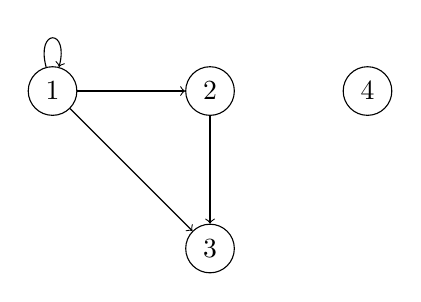
\begin{tikzpicture}[->,node distance=2cm]
  \node[draw,circle] (A) {$1$};
  \node[draw,circle] (B) [right of=A] {$2$};
  \node[draw,circle] (C) [below of=B] {$3$};
  \node[draw,circle] (D) [right of=B] {$4$};
  \draw (A) to [loop above]  (A);
  \draw (A) to  (B);
  \draw (A) to  (C);
  \draw (B) to  (C);
  \end{tikzpicture}
\intertext{આ આલેખ $\tuple{V', E}$થી જુદો છે,
  જેમાં $V' = \{1, 2, 3\}$ છે અને જે આવો દેખાય છે:}
& 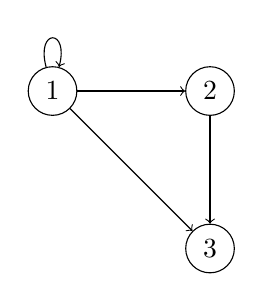
\begin{tikzpicture}[->,node distance=2cm]
  \node[draw,circle] (A) {$1$};
  \node[draw,circle] (B) [right of=A] {$2$};
  \node[draw,circle] (C) [below of=B] {$3$};
  \draw (A) to [loop above]  (A);
  \draw (A) to  (B);
  \draw (A) to  (C);
  \draw (B) to  (C);
  \end{tikzpicture}
\end{align*}
\end{ex}

\begin{prob}
  ગણ $\{1, 2, 3, 4\}$ પરના કરતાં-નાનું-અથવા-સમાન
  સંબંધ $\le$ને આલેખ તરીકે લો અને તેને અનુરૂપ આકૃતિ દોરો.
\end{prob}
% END OLP-0017
\endgroup


\begingroup
\makeatletter\def\ol@sectioncs{section}\makeatother

% BEGIN OLP-0018
\olfileid{sfr}{rel}{tre}
\olsection{વૃક્ષો}
\phantomsection\label{guunit:OLP-0018}


તર્કશાસ્ત્રના બધા ભાગોમાં મહત્વનો ભાગ ભજવતો આંશિક ક્રમનો
એક ખાસ પ્રકાર \emph{વૃક્ષ} છે. તર્કશાસ્ત્રના પ્રાથમિક ભાગોમાં
સાંત વૃક્ષો આવે છે: દાખલા તરીકે, સૂત્રોને વાક્યરચના
વૃક્ષમાં તેમના વિઘટન દ્વારા સમજી શકાય છે, જ્યારે ઘણી
નિષ્પત્તિ પદ્ધતિઓમાં નિષ્પત્તિઓ પણ સાંત વૃક્ષોનું
રૂપ ધરાવે છે.
વિધાનાત્મક અને પ્રથમ ક્રમના તર્કશાસ્ત્ર માટેના પૂર્ણતા પ્રમેયોની
સાબિતીમાં જ અનંત વૃક્ષો દેખાય છે, અને ગાણિતિક તર્કશાસ્ત્રમાં
સર્વત્ર તેમનો ઉપયોગ થાય છે.

ગણસિદ્ધાંતમાં વૃક્ષનો ખ્યાલ, આલેખસિદ્ધાંતમાં વૃક્ષના ખ્યાલ સાથે
ગાઢ રીતે જોડાયેલો છે. અહીં એક (સાંત) વૃક્ષનું ચિત્ર છે:

\begin{center}
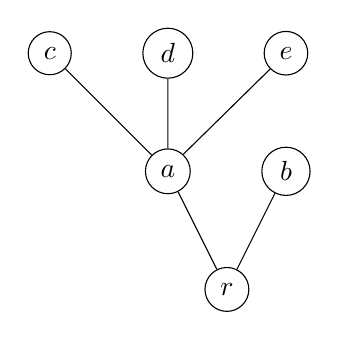
\begin{tikzpicture}[nodes={draw, circle}, -]
\node{$r$} [grow'=up]
    child { node {$a$}
        child { node {$c$} }
        child { node {$d$} }
        child { node {$e$} }
    }
    child { node {$b$} };
\end{tikzpicture}
\end{center}

સૌથી નીચેની ગાંઠ $r$ મૂળ છે. $r$ સિવાયની દરેક ગાંઠની
તરત નીચે બરાબર એક જનક ગાંઠ છે.
ગાંઠ $x$થી ધારોને અનુસરીને ઉપર જતાં ગાંઠ $y$ સુધી પહોંચી
શકાય ત્યારે $x$નો $y$ સાથેનો સંબંધ,
$x$ એ $y$નો \emph{પૂર્વજ} છે એમ સમજી શકાય.

વૃક્ષમાં પૂર્વજનો સંબંધ કડક આંશિક ક્રમ છે.
આ પરથી ગણસિદ્ધાંતની વ્યાખ્યા આપવાની પ્રેરણા મળે છે.
તે રજૂ કરવા માટે આપણને બે ખ્યાલો જોઈએ.
$\le$ વડે આંશિક ક્રમમાં ગોઠવેલા ગણ $A$માં
\emph{લઘુતમ ઘટક} એવો ઘટક $x \in A$ છે
કે દરેક $y \in A$ માટે $x \le y$.
ગણ $\le$ વડે \emph{સુક્રમિત} હોય જો તેના દરેક
અરિક્ત ઉપગણમાં લઘુતમ ઘટક હોય.

\begin{defn}[વૃક્ષ]
\emph{વૃક્ષ} એવો જોડ $T = \tuple{A, \le}$ છે કે $A$ એક ગણ છે
અને $\le$ એ $A$ પરનો આંશિક ક્રમ છે, જેમાં એકમાત્ર લઘુતમ
ઘટક $r \in A$ છે (જેને \emph{મૂળ} કહે છે), અને
દરેક $x \in A$ માટે ગણ $\Setabs{y}{y \le x}$
એ $\le$ વડે સુક્રમિત છે.
\end{defn}

\begin{defn}[અનુગામીઓ]
ધારો કે $T = \tuple{A, \le}$ વૃક્ષ છે.
જો $x,y \in A$, $x < y$, અને $x < z < y$
થાય એવો કોઈ $z \in A$ ન હોય, તો આપણે કહીએ છીએ કે
$y$ એ $x$નો \emph{અનુગામી} છે.
\end{defn}

$x \in A$ના અનુગામીઓને તેની \emph{સંતાન ગાંઠો} પણ કહે છે.
જો $y$ એ $x$નો અનુગામી હોય, તો આપણે $x$ને $y$નો
\emph{પુરોગામી} અથવા \emph{જનક} કહીએ છીએ.

\begin{prop}
જો $\tuple{A,\le}$ વૃક્ષ હોય, તો મૂળ સિવાયના
દરેક $x \in A$નો વધુમાં વધુ એક પુરોગામી હોય.
\end{prop}

\begin{proof}
  ધારો કે $y_1 < x$ અને $y_2 < x$ અને $y_1 \neq y_2$.
  તો $\{y_1, y_2\} \subseteq \Setabs{z}{z<x}$.
  $\Setabs{z}{z<x}$ એ $\le$ વડે સુક્રમિત હોવાથી,
  તેના ઉપગણ $\{y_1, y_2\}$માં લઘુતમ ઘટક છે,
  જે દેખીતી રીતે કાં $y_1$ અથવા $y_2$ હોવો જોઈએ.
  તેથી કાં $y_1 \le y_2$ અથવા $y_2 \le y_1$.
  આપણે $y_1 \neq y_2$ ધાર્યું હતું, તેથી ખરેખર
  કાં $y_1 < y_2$ અથવા $y_2 < y_1$.
  આપણે $y_1 < x$ અને $y_2 < x$ ધાર્યું હોવાથી,
  વધુમાં કાં $y_1 < y_2 < x$ અથવા $y_2 < y_1 < x$.
  તેથી $y_1$ અને $y_2$ બંને $x$ના પુરોગામી હોઈ શકે નહીં.
\end{proof}

\begin{defn}
વૃક્ષ $T = \tuple{A, \le}$ \emph{અનંત} કહેવાય જો $A$
અનંત ગણ હોય, અને નહિતર \emph{સાંત} કહેવાય.
જો $T$માં દરેક $x \in A$ના માત્ર સાંત સંખ્યામાં અનુગામીઓ હોય,
તો આપણે કહીએ છીએ કે $T$ \emph{સાંત શાખનવાળું} છે.
\end{defn}

\begin{defn}[શાખાઓ]
વૃક્ષ $T = \tuple{A, \le}$ આપેલું હોય ત્યારે,
$T$ની \emph{શાખા} એ $T$માં સમાવેશની દૃષ્ટિએ મહત્તમ શૃંખલા છે,
એટલે કે, એવો ગણ $B \subseteq A$ કે કોઈ પણ
$x, y \in B$ માટે કાં $x \le y$ અથવા $y \le x$,
અને કોઈ પણ $z \in X \setminus B$ માટે એવો
$u \in B$ અસ્તિત્વ ધરાવે છે કે ન તો $z \le u$, ન તો $u \le z$.
આપણે $T$ની બધી શાખાઓના ગણને દર્શાવવા $[T]$ વાપરીએ છીએ.
\end{defn}

\begin{ex}
સાંત શાખનવાળા વૃક્ષનું એક સુપ્રસિદ્ધ ઉદાહરણ એ $0$ અને $1$ના
સાંત અનુક્રમોનું \emph{અનંત દ્વિઆધારી વૃક્ષ} છે,
જેને ક્યારેક $\{0,1\}^*$ અથવા $\Bin^*$થી દર્શાવવામાં આવે છે,
અને જે વિસ્તરણ સંબંધ $\sqsubseteq$ વડે ક્રમિત છે
(દા.ત., $101 \sqsubseteq 101101$).
કોઈ પણ દ્વિઆધારી પ્રતીકશ્રેણીને અંતે $0$ કે $1$ ઉમેરીને
હંમેશાં વિસ્તારી શકાય છે, તેથી આ વૃક્ષમાં અનંત સંખ્યામાં
ઘટકો છે: દરેક ઘટક $s$ના બરાબર બે અનુગામી $s0$ અને $s1$ છે.
તેનું મૂળ ખાલી અનુક્રમ $\emptyseq$ છે.
\end{ex}

\begin{ex}
થોડું વધુ સામાન્ય રીતે, વિસ્તરણ સંબંધ $\sqsubseteq$ સાથે
પ્રાકૃતિક સંખ્યાઓના સાંત અનુક્રમોનો ગણ $\Nat^*$ પણ વૃક્ષ છે.
તે દેખીતી રીતે સાંત શાખનવાળું નથી: દરેક $s \in \Nat^*$ના
અનંત સંખ્યામાં અનુગામી $sn$ છે, દરેક $n \in \Nat$ માટે એક.
$\sqsubseteq$ હેઠળ સંવૃત એવો દરેક $A \subseteq \Nat^*$
એ $\Nat^*$નું \emph{ઉપવૃક્ષ} છે.
(એટલે કે, $A$ એવો છે કે જો $s \in A$ અને
$s' \sqsubseteq s$, તો $s' \in A$ પણ.)
બધાં સાંત વૃક્ષોને $\Nat^*$નાં સાંત ઉપવૃક્ષો તરીકે રજૂ કરી શકાય છે.
\end{ex}

\begin{prop}[કેનિગનું સહાયક પ્રમેય]
જો $T = \tuple{A,\le}$ સાંત શાખનવાળું અનંત વૃક્ષ હોય,
તો $T$ને અનંત શાખા હોય છે.
\end{prop}

સંગણનીયતાના સિદ્ધાંતમાં વ્યાપકપણે વપરાતો કેનિગના સહાયક
પ્રમેયનો એક વિશેષ કિસ્સો, જેને \emph{નબળું કેનિગ સહાયક પ્રમેય}
કહે છે, આ છે: $\{0,1\}^*$ના કોઈ પણ અનંત ઉપવૃક્ષને
અનંત શાખા હોય છે.
% END OLP-0018
\endgroup


\begingroup
\makeatletter\def\ol@sectioncs{section}\makeatother

% BEGIN OLP-0019
\olfileid{sfr}{rel}{ops}
\olsection{સંબંધો પરની ક્રિયાઓ}
\phantomsection\label{guunit:OLP-0019}


સંબંધોમાં ફેરફાર કરવો અથવા તેમને ભેગા કરવા ઘણી વાર ઉપયોગી
બને છે. \olref[sfr][rel][ord]{prop:stricttopartial}માં આપણે
સંબંધોના \emph{યોગગણ}નો વિચાર કર્યો હતો, જે બે સંબંધોને
જોડના ગણ તરીકે લઈએ ત્યારે તેમનો યોગગણ જ છે.
એ જ રીતે, \olref[sfr][rel][ord]{prop:partialtostrict}માં
આપણે સંબંધોના સાપેક્ષ તફાવતનો વિચાર કર્યો હતો.
અહીં સંબંધો પર કરી શકાય તેવી કેટલીક બીજી ક્રિયાઓ આપેલી છે.

\begin{defn}\ollabel{relationoperations}
ધારો કે $R$, $S$ સંબંધો છે, અને $A$ કોઈ પણ ગણ છે.

$R$નો \emph{વ્યસ્ત} એ
$R^{-1} = \Setabs{\tuple{y, x}}{\tuple{x, y} \in R}$ છે.

$R$ અને $S$નો \emph{સાપેક્ષ ગુણાકાર} એ
$(R \mid S) = \{\tuple{x, z} : \exists y(Rxy \land Syz)\}$ છે.

$R$નું $A$ પર \emph{મર્યાદન} એ
$\funrestrictionto{R}{A}= R \cap A^2$ છે.

$R$ને $A$ પર \emph{લાગુ પાડતાં મળતો ગણ} એ
$\funimage{R}{A} = \{y : (\exists x \in A)Rxy\}$ છે.
\end{defn}

\begin{ex}
ધારો કે $S \subseteq \Int^2$ એ $\Int$ પરનો અનુગામી સંબંધ છે,
એટલે કે $S = \Setabs{\tuple{x, y} \in \Int^2}{x + 1 = y}$,
જેથી $Sxy$ તો અને તો જ $x + 1 = y$.

$S^{-1}$ એ $\Int$ પરનો પુરોગામી સંબંધ છે,
એટલે કે $\Setabs{\tuple{x,y}\in\Int^2}{x -1 =y}$.

$S\mid S$ એ
$ \Setabs{\tuple{x,y}\in\Int^2}{x + 2 =y}$ છે.

$\funrestrictionto{S}{\Nat}$ એ $\Nat$ પરનો અનુગામી સંબંધ છે.

$\funimage{S}{\{1,2,3\}}$ એ $\{2, 3, 4\}$ છે.
\end{ex}

\begin{defn}[પરંપરિત સંવરણ]ધારો કે $R \subseteq A^2$ દ્વિઘટકી સંબંધ છે.

$R$નું \emph{પરંપરિત સંવરણ} એ
$R^+ = \bigcup_{0 < n \in \Nat} R^n$ છે,
જ્યાં આપણે પુનરાવર્તી રીતે $R^1 = R$ અને
$R^{n+1} = R^n \mid R$ વ્યાખ્યાયિત કરીએ છીએ.

$R$નું \emph{સ્વવાચક પરંપરિત સંવરણ} એ
$R^* = R^+ \cup \Id{A}$ છે.
\end{defn}

\begin{ex}
અનુગામી સંબંધ $S \subseteq \Int^2$ લો.
$S^2xy$ તો અને તો જ $x + 2 = y$,
$S^3xy$ તો અને તો જ $x + 3 = y$, વગેરે.
તેથી $S^+xy$ તો અને તો જ કોઈક $n \geq 1$ માટે
$x + n = y$. બીજા શબ્દોમાં, $S^+xy$ તો અને તો જ $x < y$,
અને $S^*xy$ તો અને તો જ $x \le y$.
\end{ex}

\begin{prob}
$R$નું પરંપરિત સંવરણ ખરેખર પરંપરિત છે તે દર્શાવો.
\end{prob}
% END OLP-0019
\endgroup


\OLEndChapterHook
% END OLP-0011
\endgroup


\begingroup
\makeatletter\def\ol@sectioncs{section}\makeatother

% BEGIN OLP-0020
\olchapter{sfr}{fun}{વિધેયો}
\olchapterid{sfr}{fun}
\phantomsection\label{guunit:OLP-0020}


\begingroup
\makeatletter\def\ol@sectioncs{section}\makeatother

% BEGIN OLP-0021
\olfileid{sfr}{fun}{bas}
\olsection{પાયાની બાબતો}
\phantomsection\label{guunit:OLP-0021}


\begin{explain}
\emph{વિધેય} એવું નિરૂપણ છે જે આપેલા ગણના દરેક ઘટકને
કોઈ (બીજા) આપેલા ગણના ચોક્કસ ઘટક પર મોકલે છે.
દાખલા તરીકે, $1$~ઉમેરવાની ક્રિયા એક વિધેય વ્યાખ્યાયિત કરે છે:
દરેક સંખ્યા~$n$નું નિરૂપણ અનન્ય સંખ્યા~$n+1$ પર થાય છે.

વધુ સામાન્ય રીતે, વિધેયો આગત તરીકે જોડ, ત્રિજોડ વગેરે લઈ
કોઈ પ્રકારનું નિર્ગત આપી શકે છે. પાયાના અંકગણિતમાંથી આપણને
ઘણાં વિધેયો પરિચિત છે. દાખલા તરીકે, સરવાળો અને ગુણાકાર
વિધેયો છે. તેઓ બે સંખ્યાઓ લે છે અને ત્રીજી સંખ્યા આપે છે.

આ ગાણિતિક, અમૂર્ત અર્થમાં વિધેય એક \emph{કાળી પેટી} છે:
કયા આગત સાથે કયું નિર્ગત જોડાયેલું છે એટલું જ મહત્ત્વનું છે,
નિર્ગતની ગણતરી કરવાની પદ્ધતિ નહીં.
\end{explain}

\begin{defn}[વિધેય]
\emph{વિધેય} $f \colon A \to B$ એ $A$ના દરેક ઘટકનું
$B$ના કોઈ ઘટક પરનું નિરૂપણ છે.

આપણે $A$ને $f$નો \emph{પ્રદેશ} અને $B$ને $f$નો
\emph{સહપ્રદેશ} કહીએ છીએ. $A$ના ઘટકોને $f$નાં
આગતો અથવા \emph{દલીલો} કહે છે; અને $f$ દ્વારા દલીલ~$x$ સાથે
જોડાતા $B$ના ઘટકને દલીલ~$x$ માટેની
\emph{$f$ની કિંમત} કહે છે, જેને $f(x)$ લખાય છે.

$f$નો \emph{વિસ્તાર} $\ran{f}$ એ સહપ્રદેશનો એવો ઉપગણ છે
જેમાં કોઈક દલીલ માટેની $f$ની કિંમતો આવે છે;
$\ran{f} =
\Setabs{f(x)}{x \in A}$.
\end{defn}

\olref{fig:function}માંનું ચિત્ર વિધેયો વિશે વિચારવામાં મદદરૂપ
થઈ શકે છે. ડાબી બાજુનો લંબવૃત્ત વિધેયનો \emph{પ્રદેશ}
દર્શાવે છે; જમણી બાજુનો લંબવૃત્ત તેનો \emph{સહપ્રદેશ}
દર્શાવે છે; અને તીર પ્રદેશની \emph{દલીલ}થી સહપ્રદેશની
તેને અનુરૂપ \emph{કિંમત} તરફ જાય છે.

\begin{figure}
  \olasset{assets/diagrams/function.tikz}
  \caption{વિધેય એ એક ગણના દરેક ઘટકનું બીજા ગણના
    ઘટક પરનું નિરૂપણ છે. તીર પ્રદેશની દલીલથી
    સહપ્રદેશની તેને અનુરૂપ કિંમત તરફ જાય છે.}
  \ollabel{fig:function}
\end{figure}

\begin{ex}
ગુણાકાર પ્રાકૃતિક સંખ્યાઓની જોડને આગત તરીકે લે છે અને
પ્રાકૃતિક સંખ્યાઓને નિર્ગત તરીકે આપે છે. તેથી તે
$\Nat \times \Nat$ (પ્રદેશ)થી $\Nat$ (સહપ્રદેશ)માં જાય છે.
તેનો વિસ્તાર પણ $\Nat$ છે, કારણ કે દરેક $n \in \Nat$
એ $n \times 1$ છે.
\end{ex}

\begin{ex}
ગુણાકાર વિધેય છે, કારણ કે તે દરેક આગતને---પ્રાકૃતિક સંખ્યાઓની
દરેક જોડને---એક જ નિર્ગત સાથે જોડે છે:
$\times \colon \Nat^2 \to
\Nat$. તેનાથી વિપરીત, પ્રાકૃતિક સંખ્યા~$n$ને
$x^2 = n$ થાય એવી વાસ્તવિક સંખ્યા~$x$ પર મોકલતું નિરૂપણ
વિધેયાત્મક નથી, કારણ કે દરેક ધન પૂર્ણાંક~$n$નાં બે વર્ગમૂળ
છે: $\sqrt{n}$ અને~$-\sqrt{n}$. માત્ર અનૃણ (મુખ્ય) વર્ગમૂળ આપીને
આ નિરૂપણને વિધેયાત્મક બનાવી શકીએ:
$\sqrt{\phantom{X}} \colon
\Nat \to \Real$.
\end{ex}
\sourcecorrection{OLFUN-002}{મૂળની \texttt{function-basics.tex}, પંક્તિઓ
64--71માં પ્રદેશમાં શૂન્યનો સમાવેશ હોવા છતાં ``ધન વર્ગમૂળ'' કહેવાયું છે.
અહીં શૂન્યને પણ આવરી લેતું ``અનૃણ (મુખ્ય) વર્ગમૂળ'' લખ્યું છે.}

\begin{ex}
વર્ગના દરેક વિદ્યાર્થીને તેના અંતિમ ગુણાંક સાથે જોડતો સંબંધ
વિધેય છે---એક જ વર્ગમાં કોઈ વિદ્યાર્થીને બે જુદા અંતિમ
ગુણાંક મળી શકે નહીં. વર્ગના દરેક વિદ્યાર્થીને તેનાં
માતાપિતા સાથે જોડતો સંબંધ વિધેય નથી: વિદ્યાર્થીઓને
શૂન્ય, બે કે વધુ માતાપિતા હોઈ શકે છે.
\end{ex}

\begin{explain}
દરેક સંભવિત દલીલ માટે વિધેયની કિંમત શું છે તે કોઈ ચોક્કસ
રીતે જણાવીને આપણે વિધેયો વ્યાખ્યાયિત કરી શકીએ છીએ.
તે માટે સૂત્ર આપી શકાય, કિંમતની ગણતરી કરવાની પદ્ધતિ
વર્ણવી શકાય, અથવા દરેક દલીલની કિંમતોની યાદી આપી શકાય.
વિધેયને ગમે તે રીતે વ્યાખ્યાયિત કરીએ, દરેક દલીલ માટે
એક અને માત્ર એક કિંમત નક્કી કરી છે તેની ખાતરી કરવી જોઈએ.
\end{explain}

\begin{ex}
$f(x) = x+1$ થાય તે રીતે $f \colon \Nat \to \Nat$
વ્યાખ્યાયિત કરીએ. આ વ્યાખ્યા $f$ને એવું વિધેય બનાવે છે
જે પ્રાકૃતિક સંખ્યાઓ લે છે અને પ્રાકૃતિક સંખ્યાઓ આપે છે.
તે જણાવે છે કે પ્રાકૃતિક સંખ્યા~$x$ આપતાં $f$ તેનું
અનુગામી~$x+1$ આપશે.
આ કિસ્સામાં સહપ્રદેશ $\Nat$ એ $f$નો વિસ્તાર નથી,
કારણ કે પ્રાકૃતિક સંખ્યા~$0$ કોઈ પ્રાકૃતિક સંખ્યાનું
અનુગામી નથી. $f$નો વિસ્તાર બધા ધન પૂર્ણાંકોનો ગણ
$\Int^{+}$ છે.
\end{ex}

\begin{ex}\ollabel{examplefunext}
$g(x) = x+2-1$ થાય તે રીતે $g \colon \Nat \to \Nat$
વ્યાખ્યાયિત કરીએ. આ જણાવે છે કે $g$ પ્રાકૃતિક સંખ્યાઓ
લેતું અને પ્રાકૃતિક સંખ્યાઓ આપતું વિધેય છે.
પ્રાકૃતિક સંખ્યા~$x$ આપતાં $g$, $x$ના અનુગામીના
અનુગામીનો પુરોગામી, એટલે કે $x+1$, આપશે.
\end{ex}
\sourcecorrection{OLFUN-003}{મૂળની \texttt{function-basics.tex}, પંક્તિઓ
103--107માં આગતનું નામ પહેલાં \(n\) અને પછી \(x\) છે. વ્યાખ્યા અને
પછીના સૂત્ર સાથે સુસંગત રહે તે માટે અહીં સર્વત્ર \(x\) વાપર્યું છે.}

\begin{explain}
આપણે હમણાં જુદી \emph{વ્યાખ્યાઓ} ધરાવતા બે વિધેયો,
$f$ અને $g$, જોયાં. જોકે, આ \emph{એક જ વિધેય} છે.
કારણ કે કોઈ પણ પ્રાકૃતિક સંખ્યા~$n$ માટે
$f(n) = n+1 = n+2-1 =
g(n)$ થાય છે. બીજા શબ્દોમાં, $f$ અને~$g$ માટેની આપણી
વ્યાખ્યાઓ જુદાં સમીકરણો દ્વારા એક જ નિરૂપણ નક્કી કરે છે.
આમ, ગર્ભિત રીતે આપણે વિધેયો માટે દલીલોની કિંમતો દ્વારા
નિર્ધારિત સમાનતાના સિદ્ધાંત પર આધાર રાખીએ છીએ:
\[
  \text{જો }\forall x\, f(x) = g(x)\text{, તો }f = g
\]
શરત એટલી કે $f$ અને~$g$નો પ્રદેશ અને સહપ્રદેશ એક જ હોય.
\end{explain}

\begin{ex}
આપણે કિસ્સા પાડી વિધેયો વ્યાખ્યાયિત પણ કરી શકીએ.
દાખલા તરીકે, $h \colon \Nat \to \Nat$ને આમ વ્યાખ્યાયિત
કરી શકીએ:
\[
h(x) =
\begin{cases}
  \frac{x}{2} & \text{જો $x$ યુગ્મ હોય} \\
  \frac{x+1}{2} & \text{જો $x$ અયુગ્મ હોય.}
\end{cases}
\]
દરેક પ્રાકૃતિક સંખ્યા યુગ્મ કે અયુગ્મ હોવાથી, આ વિધેયનું
નિર્ગત હંમેશાં પ્રાકૃતિક સંખ્યા હશે. એટલું યાદ રાખો કે
કિસ્સા પાડી વિધેય વ્યાખ્યાયિત કરો ત્યારે દરેક સંભવિત
આગત ચોક્કસ એક કિસ્સામાં આવવું જોઈએ. કેટલીક વાર
કિસ્સાઓ બધા આગતોને આવરી લે છે અને પરસ્પર અલગ છે
તે સાબિત કરવું જરૂરી બનશે.
\end{ex}
% END OLP-0021
\endgroup


\begingroup
\makeatletter\def\ol@sectioncs{section}\makeatother

% BEGIN OLP-0022
\olfileid{sfr}{fun}{kin}
\olsection{વિધેયોના પ્રકારો}
\phantomsection\label{guunit:OLP-0022}


\begin{explain}
આપણને વારંવાર મળતા વિધેયોના કેટલાક પ્રકારોનું
વર્ગીકરણ રજૂ કરવું ઉપયોગી થશે.

શરૂઆતમાં એવાં વિધેયો લઈએ જેમના સહપ્રદેશનો દરેક સભ્ય
વિધેયની કિંમત હોય. આવાં વિધેયોને વ્યાપ્ત કહે છે;
તેમને \olref{fig:surjective} પ્રમાણે ચિત્રમાં દર્શાવી શકાય.

\begin{figure}
  \olasset{assets/diagrams/surjective.tikz}
  \caption{વ્યાપ્ત વિધેયના સહપ્રદેશનો દરેક
    ઘટક તેની કિંમત હોય છે.}
  \ollabel{fig:surjective}
\end{figure}
\end{explain}

\begin{defn}[વ્યાપ્ત વિધેય]
વિધેય $f \colon A \rightarrow B$ \emph{વ્યાપ્ત}
હોય જો અને માત્ર જો $B$ એ $f$નો વિસ્તાર પણ હોય, એટલે કે
દરેક $y \in B$ માટે ઓછામાં ઓછો એક $x \in A$
એવો હોય કે $f(x) = y$; અથવા પ્રતીકોમાં:
\[
  (\forall y \in B)(\exists x \in A)f(x) = y.
\]
આવા વિધેયને $A$થી $B$માંનું વ્યાપ્ત વિધેય કહીએ છીએ.
\end{defn}

\begin{explain}
$f$ એ વ્યાપ્ત વિધેય છે તે બતાવવા, તમારે બતાવવું પડે
કે $f$ના સહપ્રદેશની દરેક વસ્તુ કોઈક આગત $x$ માટે
$f(x)$ની કિંમત છે.

નોંધો કે કોઈ પણ વિધેય વ્યાપ્ત વિધેય
\emph{ઉત્પન્ન કરે છે}. કારણ કે આપેલા વિધેય
$f \colon A \to B$ માટે $f'(x) = f(x)$ દ્વારા
$f' \colon A \to \ran{f}$ વ્યાખ્યાયિત કરીએ.
$\ran{f}$ની \emph{વ્યાખ્યા} જ
$\Setabs{f(x) \in B}{x \in A}$ હોવાથી આ વિધેય
$f'$ ચોક્કસ વ્યાપ્ત વિધેય છે.
\end{explain}

\begin{explain}
કોઈ પણ વિધેય દરેક સંભવિત આગતને અનન્ય નિર્ગત પર મોકલે છે.
પરંતુ એવાં વિધેયો પણ છે જે જુદાં આગતોને કદી એક જ
નિર્ગત પર મોકલતાં નથી. આવાં વિધેયોને એક-એક
કહે છે; તેમને \olref{fig:injective} પ્રમાણે ચિત્રમાં
દર્શાવી શકાય.
\begin{figure}
  \olasset{assets/diagrams/injective.tikz}
  \caption{એક-એક વિધેય કદી બે જુદી દલીલોને
    એક જ કિંમત પર મોકલતું નથી.}
  \ollabel{fig:injective}
\end{figure}
\end{explain}

\begin{defn}[એક-એક વિધેય]
વિધેય $f \colon A \rightarrow B$ \emph{એક-એક}
હોય જો અને માત્ર જો દરેક $y \in B$ માટે વધુમાં વધુ
એક $x \in A$ એવો હોય કે $f(x) = y$.
આવા વિધેયને $A$થી $B$માંનું એક-એક વિધેય કહીએ છીએ.
\end{defn}

\begin{explain}
$f$ એ એક-એક વિધેય છે તે બતાવવા, તમારે બતાવવું પડે
કે $f$ના પ્રદેશના કોઈ પણ ઘટકો $x$ અને $y$
માટે, જો $f(x)=f(y)$ હોય, તો $x=y$ થાય છે.
\end{explain}

\begin{ex}
$f(x) = 1$ દ્વારા આપેલું અચળ વિધેય
$f\colon \Nat \to \Nat$ એક-એક પણ નથી
અને વ્યાપ્ત પણ નથી.

$f(x) = x$ દ્વારા આપેલું તદેવ વિધેય
$f\colon \Nat \to \Nat$ એક-એક અને
વ્યાપ્ત બંને છે.

$f(x) = x+1$ દ્વારા આપેલું અનુગામી વિધેય
$f \colon \Nat \to \Nat$ એક-એક છે,
પરંતુ વ્યાપ્ત નથી.

નીચે મુજબ વ્યાખ્યાયિત વિધેય $f \colon \Nat \to \Nat$:
\[
  f(x) =
  \begin{cases}
    \frac{x}{2} & \text{જો $x$ યુગ્મ હોય} \\
    \frac{x+1}{2} & \text{જો $x$ અયુગ્મ હોય.}
  \end{cases}
\]
વ્યાપ્ત છે, પરંતુ એક-એક નથી.
\end{ex}

\begin{explain}
ઘણી વાર આપણે એક-એક અને વ્યાપ્ત બંને
હોય એવાં વિધેયો લેવા માગીએ છીએ. આવાં વિધેયોને
એક-એક અને વ્યાપ્ત કહીએ છીએ. તેઓ
\olref{fig:bijective}માં દર્શાવેલા વિધેય જેવાં દેખાય છે.
એક-એક વ્યાપ્ત વિધેયોને ક્યારેક \emph{પરસ્પર એક-એક સંગતતાઓ}
પણ કહે છે, કારણ કે તેઓ સહપ્રદેશના ઘટકોને પ્રદેશના
ઘટકો સાથે અનન્ય રીતે જોડે છે.
\begin{figure}
  \olasset{assets/diagrams/bijective.tikz}
  \caption{એક-એક અને વ્યાપ્ત વિધેય સહપ્રદેશના ઘટકોને
    પ્રદેશના ઘટકો સાથે અનન્ય રીતે જોડે છે.}
  \ollabel{fig:bijective}
\end{figure}
\end{explain}

\begin{defn}[એક-એક વ્યાપ્ત વિધેય]
વિધેય $f \colon A \to B$ \emph{એક-એક અને વ્યાપ્ત} હોય
જો અને માત્ર જો તે વ્યાપ્ત અને એક-એક
બંને હોય. આવા વિધેયને $A$થી $B$માંનું
(અથવા $A$ અને~$B$ વચ્ચેનું) એક-એક વ્યાપ્ત વિધેય કહીએ છીએ.
\end{defn}
% END OLP-0022
\endgroup


\begingroup
\makeatletter\def\ol@sectioncs{section}\makeatother

% BEGIN OLP-0023
\olfileid{sfr}{fun}{rel}

\olsection{સંબંધો તરીકે વિધેયો}
\phantomsection\label{guunit:OLP-0023}


\begin{explain}
$A$ના ઘટકોને $B$ના ઘટકો પર મોકલતું
વિધેય સ્પષ્ટપણે $A$ અને~$B$ વચ્ચે સંબંધ વ્યાખ્યાયિત
કરે છે: $x$ અને $y$ વચ્ચે આ સંબંધ હોય જો અને માત્ર જો
$f(x) = y$ હોય. હકીકતમાં, દાખલા તરીકે ગણિતના પાયાના
ઘટકોની સંખ્યા ઘટાડવામાં રસ હોય તો, આપણે વિધેય~$f$ને
આ સંબંધ સાથે, એટલે કે જોડોના ગણ સાથે, \emph{એકરૂપ}
પણ ગણી શકીએ. ત્યારે પ્રશ્ન ઊભો થાય છે: કયા સંબંધો
આ રીતે વિધેયો વ્યાખ્યાયિત કરે છે?
\end{explain}

\begin{defn}[વિધેયનો આલેખ] ધારો કે $f\colon A \to B$
વિધેય છે. $f$નો \emph{આલેખ} એ નીચે પ્રમાણે વ્યાખ્યાયિત
સંબંધ $R_f \subseteq A \times B$ છે:
\[
R_f = \Setabs{\tuple{x,y}}{f(x) = y}.
\]
\end{defn}

\begin{explain}
ઘટકો દ્વારા નિર્ધારિત સમાનતાના સિદ્ધાંતથી વિધેયનો
આલેખ અનન્ય રીતે નક્કી થાય છે. વધુમાં, ગણો માટેનો
આ સિદ્ધાંત વિધેયો માટેના ગર્ભિત સમાનતાના સિદ્ધાંતને
તરત સમર્થન આપે છે: જો $f$ અને~$g$નો પ્રદેશ અને
સહપ્રદેશ એક જ હોય, તો બધી દલીલો માટેની કિંમતો
સરખી હોય ત્યારે તેઓ એક જ વિધેય હોય છે.

એ જ રીતે, સંબંધ “વિધેયાત્મક” હોય, તો તે કોઈ
વિધેયનો આલેખ છે.
\end{explain}

\begin{prop}\ollabel{prop:graph-function}
ધારો કે $R \subseteq A \times B$ એવો છે કે:
\begin{enumerate}
\item જો $Rxy$ અને $Rxz$ હોય, તો $y = z$; અને
\item દરેક $x \in A$ માટે કોઈક $y \in B$ એવો છે
કે $\tuple{x,
y} \in R$.
\end{enumerate}
તો $R$ એ $f(x) = y$ જો અને માત્ર જો $Rxy$
દ્વારા વ્યાખ્યાયિત વિધેય $f\colon A \to B$નો આલેખ છે.
\end{prop}

\begin{proof}
ધારો કે $Rxy$ થાય એવો $y$ છે. જો $Rxz$ થાય એવો
બીજો $z \neq
y$ હોત, તો $R$ પરની શરતનો ભંગ થાત.
આથી, $Rxy$ થાય એવો $y$ હોય, તો આ $y$ અનન્ય છે,
અને તેથી $f$ સુવ્યાખ્યાયિત છે. સ્પષ્ટપણે $R_f = R$.
\end{proof}

\begin{explain}
દરેક વિધેય $f\colon A \to B$નો આલેખ હોય છે, એટલે કે
$f(x) = y$ દ્વારા વ્યાખ્યાયિત $A
\times B$માં સમાયેલો સંબંધ. બીજી તરફ,
\olref{prop:graph-function}માં આપેલા ગુણધર્મો ધરાવતો
દરેક સંબંધ~$R
\subseteq A \times B$ કોઈ વિધેય~$f \colon A \to
B$નો આલેખ છે. વિધેયો અને તેમના આલેખો વચ્ચેના આ ગાઢ
સંબંધને કારણે આપણે વિધેયને તેના આલેખ તરીકે જ વિચારી શકીએ.
બીજા શબ્દોમાં, વિધેયોને અમુક સંબંધો સાથે, એટલે કે અમુક
બહુજોડોના ગણો સાથે, એકરૂપ ગણી શકાય.
જોકે, નોંધો કે આ “એકરૂપતા”નો
આશય \olref[sfr][rel][ref]{sec}માં જણાવ્યો હતો તેવો છે:
તે વિધેયોના તત્વમીમાંસાકીય સ્વરૂપ વિશેનો દાવો નથી;
વિધેયોને અમુક ગણો તરીકે \emph{લેવાં} અનુકૂળ છે એવી
નોંધ છે. આ અનુકૂળતાનું એક કારણ એ છે કે આપણે
હવે સંબંધો પર કરેલી ક્રિયાઓ જેવી ક્રિયાઓ વિધેયો પર
કરવાનું વિચારી શકીએ છીએ (જુઓ \olref[sfr][rel][ops]{sec}).
ખાસ કરીને:
\end{explain}
\sourcecorrection{OLFUN-004}{મૂળની \texttt{functions-relations.tex}, પંક્તિઓ
60--68માં આલેખને ``\(A\times B\) પરનો સંબંધ'' કહેવાયો છે. પ્રોજેક્ટની
પોતાની વ્યાખ્યા પ્રમાણે અહીં \(A\) અને \(B\) વચ્ચેનો, એટલે કે
\(A\times B\)માં સમાયેલો સંબંધ અભિપ્રેત છે; અનુવાદમાં એ પ્રકાર સ્પષ્ટ કર્યો છે.}

\begin{defn}\ollabel{defn:funimage}
ધારો કે $f \colon A \to B$ વિધેય છે અને $C\subseteq A$ છે.

$f$નું $C$ પરનું \emph{મર્યાદન} એ બધા $x \in C$ માટે
$(\funrestrictionto{f}{C})(x) = f(x)$ દ્વારા વ્યાખ્યાયિત
વિધેય~$\funrestrictionto{f}{C}\colon C \to B$ છે.
બીજા શબ્દોમાં, $\funrestrictionto{f}{C} = \Setabs{\tuple{x, y} \in R_f}{x \in
C}$.

$C$ પર $f$નું \emph{પ્રયોજન} એ $\funimage{f}{C} =
\Setabs{f(x)}{x \in C}$ છે. તેને $f$ હેઠળનું
$C$નું \emph{પ્રતિબિંબ} પણ કહીએ છીએ.
\end{defn}

\begin{explain}
આ વ્યાખ્યાઓ પરથી કોઈ પણ વિધેય~$f$ માટે
$\ran{f} =
\funimage{f}{\dom{f}}$ મળે છે.
\olref[sfr][rel][ops]{sec}ની
વ્યાખ્યાઓ અને વિધેયોને સંબંધો સાથે એકરૂપ ગણવાની આપણી
રીત જોતાં, આ ખ્યાલો અનુરૂપ છે. અહીં વિધેયનું મર્યાદન
માત્ર પ્રદેશને C સુધી સીમિત કરે છે; અગાઉનું સંબંધ-મર્યાદન
બંને અવયવોને C સુધી સીમિત કરે છે. પરંતુ બે બીજી
ક્રિયાઓ---વ્યસ્ત અને સાપેક્ષ ગુણાકાર---માટે થોડી વધુ
વિગત જરૂરી છે. તે \olref[inv]{sec} અને
\olref[cmp]{sec}માં આપીશું.
\end{explain}
\sourcecorrection{OLFUN-005}{મૂળની \texttt{functions-relations.tex}, પંક્તિઓ
78--100માં વિધેય-મર્યાદનની સ્પષ્ટ વ્યાખ્યા સાચી છે, પરંતુ તેને અગાઉના
બંને-અવયવવાળા સંબંધ-મર્યાદન સાથે ``ચોક્કસ'' સરખું કહેવાયું છે. અહીં
આ સામ્યની મર્યાદા સ્પષ્ટ કરી છે.}
% END OLP-0023
\endgroup


\begingroup
\makeatletter\def\ol@sectioncs{section}\makeatother

% BEGIN OLP-0024
\olfileid{sfr}{fun}{inv}
\olsection{વિધેયોનાં પ્રતિવિધેયો}
\phantomsection\label{guunit:OLP-0024}


\begin{explain}
આપણે વિધેયોને નિરૂપણો તરીકે વિચારીએ છીએ. તેથી વિધેયો
વિશે એક સ્વાભાવિક પ્રશ્ન એ છે કે નિરૂપણને “ઊલટાવી”
શકાય કે નહીં. દાખલા તરીકે, અનુગામી વિધેય
$f(x) = x + 1$ને આ અર્થમાં ઊલટાવી શકાય કે વિધેય
$g(y) = y - 1$ એ $f$ની ક્રિયાને “પાછી ફેરવે” છે.

પરંતુ સાવચેત રહેવું જોઈએ. $g$ની વ્યાખ્યા વિધેય
$\Int \to \Int$ વ્યાખ્યાયિત કરે છે, છતાં તે
\emph{વિધેય} $\Nat
\to \Nat$ વ્યાખ્યાયિત કરતી નથી, કારણ કે
$g(0) \notin \Nat$. એટલે સરળ કિસ્સામાં પણ વિધેયને
ઊલટાવી શકાય કે નહીં તે તરત સ્પષ્ટ થતું નથી;
તે પ્રદેશ અને સહપ્રદેશ પર આધાર રાખી શકે છે.

વિધેયના પ્રતિવિધેયનો ખ્યાલ આ વાતને વધુ ચોક્કસ બનાવે છે.
\end{explain}

\begin{defn}
વિધેય $g \colon B \to A$ એ વિધેય $f
\colon A \to B$નું \emph{પ્રતિવિધેય} છે જો બધા
$x \in A$ અને $y \in B$ માટે
$f(g(y)) = y$ અને $g(f(x)) = x$ થાય.
\end{defn}

જો $f$નું પ્રતિવિધેય~$g$ હોય, તો ઘણી વાર $g$ને
બદલે $f^{-1}$ લખીએ છીએ.

\begin{explain}
હવે વિધેયોને ક્યારે પ્રતિવિધેયો હોય છે તે નક્કી કરીશું.
$f\colon A \to B$ના પ્રતિવિધેય માટેનો યોગ્ય ઉમેદવાર
નીચે મુજબ “વ્યાખ્યાયિત” $g\colon B \to A$ છે:
\[
g(y) = \text{$f(x) = y$ થાય એવો “તે એક જ” $x$.}
\]
પરંતુ “વ્યાખ્યાયિત” (અને “તે એક જ”)ની આસપાસનાં
અવતરણચિહ્નો સૂચવે છે કે આ વ્યાખ્યા નથી. ઓછામાં ઓછું,
તે સંપૂર્ણ સામાન્યતાથી હંમેશાં કામ નહીં કરે. કારણ કે
આ વ્યાખ્યા વિધેય નક્કી કરે તે માટે $f(x) =
y$ થાય એવો એક અને માત્ર એક~$x$ હોવો જોઈએ---$g$નું
નિર્ગત અનન્ય રીતે નક્કી થવું જોઈએ. વધુમાં, દરેક
$y \in B$ માટે તે નક્કી થવું જોઈએ. જો $x_1$ અને
$x_2 \in
A$ એવા હોય કે $x_1 \neq x_2$ છતાં
$f(x_1) = f(x_2)$ હોય, તો $y = f(x_1) = f(x_2)$
માટે $g(y)$ અનન્ય રીતે નક્કી નહીં થાય. અને જો
$f(x) = y$ થાય એવો કોઈ~$x$ જ ન હોય, તો
$g(y)$ બિલકુલ નક્કી થતું નથી. બીજા શબ્દોમાં,
$g$ વ્યાખ્યાયિત થાય તે માટે $f$ એ એક-એક
અને વ્યાપ્ત બંને હોવું જોઈએ.

ધીમે ધીમે આગળ વધીએ. પ્રશ્નને બે ભાગમાં વહેંચીએ:
વિધેય~$f\colon A \to B$ આપેલું હોય ત્યારે
$g(f(x)) = x$ થાય એવું વિધેય $g\colon B \to A$
ક્યારે હોય? આવું $g$ એ $f$ની ક્રિયાને “પાછી ફેરવે” છે;
તેને $f$નો \emph{ડાબી બાજુનો વ્યસ્ત} કહે છે.
બીજું, $f(h(y)) = y$ થાય એવું વિધેય
$h\colon B \to A$ ક્યારે હોય? આવા $h$ને
$f$નો \emph{જમણી બાજુનો વ્યસ્ત} કહે છે---$f$
એ $h$ની ક્રિયાને “પાછી ફેરવે” છે.
\end{explain}

\begin{prop}
જો $f\colon A \to B$ એ એક-એક હોય અને તેનો પ્રદેશ અખાલી હોય, તો
$f$નો \emph{ડાબી બાજુનો વ્યસ્ત}~$g\colon B \to A$
હોય છે, જેથી બધા $x
\in A$ માટે $g(f(x)) = x$ થાય.
\end{prop}

\begin{proof}
ધારો કે $f\colon A \to B$ એ એક-એક છે અને તેનો પ્રદેશ અખાલી છે.
કોઈ $y \in B$ લો. જો $y \in \ran{f}$ હોય,
તો $f(x) = y$ થાય એવો $x \in A$ છે.
$f$ એ એક-એક હોવાથી આવો માત્ર એક~$x \in A$
છે. તેથી $g(y) = x$ વ્યાખ્યાયિત કરી શકીએ, એટલે કે
$g(y)$ એ $f(x)
= y$ થાય એવો “તે એક જ” $x \in A$ છે.
જો $y \notin \ran{f}$ હોય, તો તેને કોઈ પણ~$a \in A$
પર મોકલી શકીએ. એટલે એક $a \in A$ પસંદ કરી
$g\colon B \to A$ને આમ વ્યાખ્યાયિત કરી શકીએ:
\[
g(y) = \begin{cases}
    x & \text{જો $f(x) = y$ હોય}\\
    a & \text{જો $y \notin \ran{f}$ હોય.}
\end{cases}
\]
તે બધા $y \in B$ માટે વ્યાખ્યાયિત છે, કારણ કે
આવા દરેક $y \in \ran{f}$ માટે $f(x) = y$ થાય
એવો ચોક્કસ એક $x \in A$ છે. વ્યાખ્યા પ્રમાણે,
જો $y = f(x)$ હોય, તો $g(y) = x$ થાય,
એટલે કે $g(f(x)) = x$.
\end{proof}
\sourcecorrection{OLFUN-001}{મૂળની \texttt{inverses.tex}, પંક્તિઓ 62--84માં
પ્રદેશ અખાલી હોવાની શરત વિના આ વિધાન ખોટું છે: ખાલી ગણથી એક-ઘટકવાળા
ગણમાંનું ખાલી વિધેય એક-એક છે, પરંતુ તેનો ડાબી બાજુનો વ્યસ્ત નથી.
સરળ સુધારેલા વિધાનમાં પ્રદેશ અખાલી હોવાની શરત ઉમેરી છે. ચોક્કસ સામાન્ય
શરત એ છે કે પ્રદેશ અખાલી હોય અથવા સહપ્રદેશ ખાલી હોય.}

\begin{prob}
બતાવો કે જો $f\colon A \to B$નો ડાબી બાજુનો
વ્યસ્ત~$g$ હોય, તો $f$ એ એક-એક છે.
\end{prob}

\begin{prop}
જો $f\colon A \to B$ એ વ્યાપ્ત હોય, તો
$f$નો \emph{જમણી બાજુનો વ્યસ્ત}~$h\colon B \to A$
હોય છે, જેથી બધા~$y \in B$ માટે $f(h(y)) =
y$ થાય.
\end{prop}

\begin{proof}
ધારો કે $f\colon A \to B$ એ વ્યાપ્ત છે.
કોઈ $y \in
B$ લો. $f$ એ વ્યાપ્ત હોવાથી
$f(x_y)
= y$ થાય એવો $x_y \in A$ છે.
તેથી $h(y) = x_y$ વ્યાખ્યાયિત કરી શકીએ, એટલે કે
દરેક $y \in B$ માટે $f(x) = y$ થાય એવો કોઈ
$x \in A$ પસંદ કરીએ; $f$ એ વ્યાપ્ત
હોવાથી પસંદ કરવા માટે હંમેશાં ઓછામાં ઓછો એક હોય છે.
\footnote{$f$ એ વ્યાપ્ત હોવાથી દરેક~$y \in B$
માટે ગણ $\Setabs{x}{f(x) = y}$ ખાલી નથી.
$h$ની આપણી વ્યાખ્યા માટે આ દરેક ગણમાંથી એક જ $x$
પસંદ કરવો પડે છે. આ હંમેશાં શક્ય છે તે હકીકતમાં
સ્પષ્ટ નથી---આવી પસંદગીઓ કરવાની શક્યતા એક
સ્વયંસિદ્ધિ તરીકે માની લેવામાં આવે છે.
બીજા શબ્દોમાં, આ વિધાન કહેવાતી પસંદગીની સ્વયંસિદ્ધિ
ધારે છે. આ મુદ્દાને આપણે
\olref[sth][choice][]{chap}માં ફરી જોઈશું.
જોકે, ઘણા ચોક્કસ કિસ્સામાં, દાખલા તરીકે $A = \Nat$
હોય કે સાન્ત હોય, અથવા $f$ એ એક-એક અને વ્યાપ્ત હોય,
ત્યારે પસંદગીની સ્વયંસિદ્ધિ જરૂરી નથી. (ખાસ કરીને
$f$ એ એક-એક અને વ્યાપ્ત હોય ત્યારે દરેક $y \in B$
માટે ગણ $\Setabs{x}{f(x) = y}$માં ચોક્કસ એક
ઘટક હોય છે, એટલે પસંદગી કરવાની રહેતી જ નથી.)}
વ્યાખ્યા પ્રમાણે, જો $x = h(y)$ હોય,
તો $f(x) = y$ થાય; એટલે કે કોઈ પણ $y \in B$
માટે $f(h(y)) = y$.
\end{proof}

\begin{prob}
બતાવો કે જો $f\colon A \to B$નો જમણી બાજુનો
વ્યસ્ત~$h$ હોય, તો $f$ એ વ્યાપ્ત છે.
\end{prob}

\begin{explain}
અગાઉની સાબિતીના વિચારોને ભેગા કરતાં હવે મળે છે કે
દરેક એક-એક વ્યાપ્ત વિધેયને પ્રતિવિધેય હોય છે, એટલે કે
એક જ વિધેય $f$નો ડાબી અને જમણી બંને બાજુનો વ્યસ્ત હોય છે.
\end{explain}

\begin{prop}\ollabel{prop:bijection-inverse}
જો $f\colon A \to B$ એ એક-એક અને વ્યાપ્ત હોય, તો એવું
વિધેય~$f^{-1}\colon B \to A$ છે કે બધા $x \in A$
માટે $f^{-1}(f(x)) = x$ અને બધા $y \in B$
માટે $f(f^{-1}(y)) = y$ થાય.
\end{prop}

\begin{proof}
સ્વાધ્યાય.
\end{proof}

\begin{prob}
\olref[sfr][fun][inv]{prop:bijection-inverse} સાબિત કરો.
તમારે $f^{-1}$ વ્યાખ્યાયિત કરવું, તે વિધેય છે તે
બતાવવું, અને તે $f$નું પ્રતિવિધેય છે તે બતાવવું પડે;
એટલે કે બધા $x \in A$ અને $y \in B$ માટે
$f^{-1}(f(x)) = x$ અને $f(f^{-1}(y)) = y$ થાય.
\end{prob}

\begin{explain}
પ્રતિવિધેયો મેળવવાની થોડી વધુ સામાન્ય રીત છે.
આપણે \olref[kin]{sec}માં જોયું કે દરેક વિધેય $f$
બધા $x \in A$ માટે $f'(x) = f(x)$ લઈને
વ્યાપ્ત વિધેય $f'
\colon A \to \ran{f}$ ઉત્પન્ન કરે છે.
સ્પષ્ટ છે કે $f$ એ એક-એક હોય, તો
$f'$ એ એક-એક અને વ્યાપ્ત છે; તેથી
\olref{prop:bijection-inverse} પ્રમાણે તેને અનન્ય
પ્રતિવિધેય હોય છે. સંકેતપ્રયોગમાં બહુ નાની છૂટ લઈને
આપણે ક્યારેક $f'$ના પ્રતિવિધેયને માત્ર
“$f$નું પ્રતિવિધેય” કહીએ છીએ.
\end{explain}

\begin{prop}\ollabel{prop:left-right}%
બતાવો કે જો $f\colon A \to B$નો ડાબી બાજુનો
વ્યસ્ત~$g$ અને જમણી બાજુનો વ્યસ્ત~$h$ હોય,
તો $h = g$ થાય.
\end{prop}

\begin{proof}
સ્વાધ્યાય.
\end{proof}

\begin{prob}
\olref[sfr][fun][inv]{prop:left-right} સાબિત કરો.
\end{prob}

\begin{prop}\ollabel{prop:inverse-unique}
દરેક વિધેય~$f$ને વધુમાં વધુ એક પ્રતિવિધેય હોય છે.
\end{prop}

\begin{proof}
ધારો કે $g$ અને $h$ બંને $f$નાં પ્રતિવિધેયો છે.
તો ખાસ કરીને $g$ એ $f$નો ડાબી બાજુનો વ્યસ્ત
અને $h$ જમણી બાજુનો વ્યસ્ત છે.
\olref{prop:left-right} પ્રમાણે $g = h$.
\end{proof}
% END OLP-0024
\endgroup


\begingroup
\makeatletter\def\ol@sectioncs{section}\makeatother

% BEGIN OLP-0025
\olfileid{sfr}{fun}{cmp}
\olsection{વિધેયોનું સંયોજન}
\phantomsection\label{guunit:OLP-0025}


\begin{explain}
આપણે \olref[inv]{sec}માં
જોયું કે એક-એક વ્યાપ્ત વિધેય~$f$નું પ્રતિવિધેય~$f^{-1}$
પોતે એક વિધેય છે. વિધેયો પરની બીજી ક્રિયા સંયોજન છે:
આપણે બે વિધેયો $f$ અને~$g$નું સંયોજન કરીને,
એટલે કે પહેલાં $f$ અને પછી $g$ લાગુ પાડીને, નવું વિધેય
વ્યાખ્યાયિત કરી શકીએ. અલબત્ત, વિસ્તાર અને પ્રદેશ મેળ ખાતા
હોય તો જ આ શક્ય છે: $f$નો વિસ્તાર $g$ના પ્રદેશનો
ઉપગણ હોવો જોઈએ. વિધેયો
પરની આ ક્રિયા \olref[rel][ops]{sec}માં સંબંધો પરની
સાપેક્ષ ગુણાકારની ક્રિયાને અનુરૂપ છે.

સંયોજનનો ખ્યાલ સમજાવવામાં ચિત્ર મદદરૂપ થઈ શકે.
\olref{fig:composition}માં આપણે બે વિધેયો
$f \colon A \to B$ અને $g \colon B \to C$
તથા તેમનું સંયોજન~$(\comp{f}{g})$ દર્શાવીએ છીએ.
વિધેય $(\comp{f}{g}) \colon A \to C$ એ $A$ના દરેક
ઘટકને $C$ના ઘટક સાથે જોડે છે.
$A$નો ઘટક એ $C$ના કયા ઘટક
સાથે જોડાય છે તે આ રીતે નક્કી કરીએ: આગત $x \in
A$ આપેલું હોય ત્યારે પહેલાં વિધેય $f$ને $x$ પર લાગુ પાડો.
તે કોઈક $f(x)
= y \in B$ આપશે; પછી $g$ને $y$ પર લાગુ પાડો.
તે કોઈક $g(f(x)) = g(y) = z \in C$ આપશે.
\begin{figure}
  \olasset[2\olphotowidth]{assets/diagrams/composition.tikz}
  \caption{બે વિધેયો $f$ અને~$g$નું સંયોજન $g \circ f$.}
  \ollabel{fig:composition}
\end{figure}
\end{explain}

\begin{defn}[સંયોજન]
ધારો કે $f\colon A \to B$ અને $g\colon B \to C$
વિધેયો છે. $f$નું $g$ સાથેનું \emph{સંયોજન}
એ $\comp{f}{g} \colon A \to C$ છે, જ્યાં
$(\comp{f}{g})(x) = g(f(x))$.
\end{defn}

\begin{ex}
વિધેયો $f(x) = x + 1$ અને $g(x) = 2x$ લો.
$(\comp{f}{g})(x) = g(f(x))$ હોવાથી, દરેક આગત~$x$
માટે પહેલાં તેનું અનુગામી લેવું પડે અને પછી પરિણામને
બે વડે ગુણવું પડે. તેથી તેમનું સંયોજન
$(\comp{f}{g})(x) = 2(x+1)$ દ્વારા અપાય છે.
\end{ex}

\begin{prob}
બતાવો કે જો $f \colon A \to B$ અને $g \colon B \to C$
બંને એક-એક હોય, તો $\comp{f}{g}\colon A \to C$
પણ એક-એક છે.
\end{prob}

\begin{prob}
બતાવો કે જો $f \colon A \to B$ અને $g \colon B \to C$
બંને વ્યાપ્ત હોય, તો $\comp{f}{g}\colon A \to C$
પણ વ્યાપ્ત છે.
\end{prob}

\begin{prob}
ધારો કે $f \colon A \to B$ અને $g \colon B \to C$ છે.
બતાવો કે $\comp{f}{g}$નો આલેખ $R_f \mid R_g$ છે.
\end{prob}
% END OLP-0025
\endgroup



\begingroup
\makeatletter\def\ol@sectioncs{section}\makeatother

% BEGIN OLP-0026
\olfileid{sfr}{fun}{par}

\olsection{આંશિક વિધેયો}
\phantomsection\label{guunit:OLP-0026}


\begin{explain}
ક્યારેક વિધેયની વ્યાખ્યામાં છૂટ આપવી ઉપયોગી બને છે,
જેથી દરેક સંભવિત આગત માટે વિધેયનું નિર્ગત વ્યાખ્યાયિત
હોય તે જરૂરી ન રહે. આવાં નિરૂપણોને
\emph{આંશિક વિધેયો} કહે છે.
\end{explain}

\begin{defn}
\emph{આંશિક વિધેય} $f \colon A \pto B$ એવું નિરૂપણ છે
જે $A$ના દરેક ઘટકને $B$નો વધુમાં વધુ એક
ઘટક ફાળવે છે. જો $f$ એ $x \in A$ને $B$નો
કોઈ ઘટક ફાળવે, તો $f(x)$ \emph{વ્યાખ્યાયિત} છે
એમ કહીએ; અન્યથા તે \emph{અવ્યાખ્યાયિત} છે.
$f(x)$ વ્યાખ્યાયિત હોય તો $f(x) \fdefined$ લખીએ,
અન્યથા $f(x) \fundefined$ લખીએ. આંશિક વિધેય~$f$નો
\emph{પ્રદેશ} એ $A$નો એવો ઉપગણ છે જ્યાં તે
વ્યાખ્યાયિત હોય, એટલે કે
$\dom{f} = \Setabs{x \in A}{f(x) \fdefined}$.
\end{defn}

\begin{ex}
દરેક વિધેય $f\colon A \to B$ આંશિક વિધેય પણ છે.
$A$ પર સર્વત્ર વ્યાખ્યાયિત આંશિક વિધેયો---એટલે કે
અત્યાર સુધી આપણે જેને માત્ર વિધેય કહેતા આવ્યા છીએ તે---
\emph{સર્વત્ર વ્યાખ્યાયિત} વિધેયો પણ કહેવાય છે.
\end{ex}

\begin{ex}
$f(x) = 1/x$ દ્વારા આપેલું આંશિક વિધેય
$f \colon \Real \pto \Real$ એ $x = 0$ માટે
અવ્યાખ્યાયિત છે અને બાકીની બધી જગ્યાએ વ્યાખ્યાયિત છે.
\end{ex}

\begin{prob}
આપેલા $f\colon A \pto B$ માટે આંશિક વિધેય
$g\colon B \pto
A$ આ રીતે વ્યાખ્યાયિત કરો: કોઈ પણ $y \in B$ માટે,
જો $f(x) = y$ થાય એવો અનન્ય $x \in A$ હોય,
તો $g(y) = x$; અન્યથા $g(y) \fundefined$.
બતાવો કે જો $f$ એક-એક હોય, તો બધા $x \in \dom{f}$
માટે $g(f(x)) = x$ અને બધા $y \in \ran{f}$ માટે
$f(g(y)) = y$ થાય છે.
\end{prob}

\begin{defn}[આંશિક વિધેયનો આલેખ]
ધારો કે $f\colon A \pto B$ આંશિક વિધેય છે.
$f$નો \emph{આલેખ} એ નીચે મુજબ વ્યાખ્યાયિત સંબંધ
$R_f \subseteq A \times B$ છે:
\[
R_f = \Setabs{\tuple{x,y}}{f(x) = y}.
\]
\end{defn}

\begin{prop}
ધારો કે $R \subseteq A \times B$નો ગુણધર્મ એવો છે કે
જ્યારે પણ $Rxy$ અને $Rxy'$ હોય, ત્યારે $y = y'$ થાય છે.
તો $R$ એ આ રીતે વ્યાખ્યાયિત આંશિક વિધેય
$f\colon A \pto B$નો આલેખ છે: જો $Rxy$ થાય એવો $y$
હોય, તો $f(x) = y$; અન્યથા $f(x) \fundefined$.
જો $R$ \emph{સર્વાગત} પણ હોય, એટલે કે દરેક $x \in A$
માટે $Rxy$ થાય એવો કોઈ $y \in B$ હોય, તો $f$
સર્વત્ર વ્યાખ્યાયિત છે.
\end{prop}

\begin{proof}
ધારો કે $Rxy$ થાય એવો $y$ છે. જો $Rxy'$ થાય એવો
બીજો $y'
\neq y$ હોત, તો $R$ પરની શરતનો ભંગ થાત.
આથી, $Rxy$ થાય એવો $y$ હોય, તો તે $y$ અનન્ય છે;
તેથી $f$ સુવ્યાખ્યાયિત છે. સ્પષ્ટપણે $R_f = R$
અને જો $R$ સર્વાગત હોય, તો $f$ સર્વત્ર વ્યાખ્યાયિત છે.
\end{proof}
% END OLP-0026
\endgroup


\OLEndChapterHook


\begin{editorial}
આગળનો સંબંધિત અંશ મૂળના સક્રિય આયાતક્રમમાં નથી. તેને અહીં સ્પષ્ટ વૈકલ્પિક સંદર્ભમાં જાળવ્યો છે.
\end{editorial}
\begingroup
\makeatletter\def\ol@sectioncs{section}\makeatother

% BEGIN OLP-0717
\olfileid{sfr}{fun}{iso}
\olsection{એકરૂપતા}
\phantomsection\label{guunit:OLP-0717}


\begin{explain}
\emph{એકરૂપતા} એ જોડાતા ગણોની સંરચના જાળવતું એક-એક વ્યાપ્ત વિધેય છે.
સંરચના એટલે ગણોના ઘટકો વચ્ચે રહેલા સંબંધો.
બે ગણ $X=\{1,2,3\}$ અને $Y=\{4,5,6\}$ લો.
બંનેમાં અનુગામી હોવાનો, નાનું હોવાનો અને મોટું હોવાનો સંબંધ છે.
બે ગણો વચ્ચેની એકરૂપતા આ સંરચનાઓ જાળવતું એક-એક વ્યાપ્ત વિધેય છે.
એટલે એક-એક અને વ્યાપ્ત ફલન~$f \colon X
\to Y$ એકરૂપતા છે જો, ગણના કોઈ પણ બે ઘટકો માટે,
$i<j$ જો અને ફક્ત જો $f(i)<f(j)$,
$i>j$ જો અને ફક્ત જો $f(i)>f(j)$,
અને $j$ એ $i$નો અનુગામી હોય જો અને ફક્ત જો $f(j)$ એ
$f(i)$નો અનુગામી હોય.
\end{explain}

\begin{defn}[એકરૂપતા]
$U$ એ જોડી $\langle X, R\rangle$ અને $V$ એ જોડી
$\langle Y, S\rangle$ હોય, જ્યાં $X$ અને $Y$ ગણો છે અને
$R$ તથા $S$ અનુક્રમે $X$ તથા $Y$ પરના સંબંધો છે.
$X$થી $Y$માં જતું એક-એક વ્યાપ્ત વિધેય~$f$ એ $U$થી $V$માં જતી
\emph{એકરૂપતા} છે જો અને ફક્ત જો તે સંબંધની સંરચના જાળવે:
$X$ના કોઈ પણ $x_{1}$ અને $x_{2}$ માટે
$\tuple{x_1,x_2} \in R$ જો અને ફક્ત જો
$\tuple{f(x_1),f(x_2)} \in S$.
\end{defn}

\begin{ex}
બે ગણ $X=\{1,2,3\}$ અને $Y=\{4,5,6\}$ લો,
સાથે નાનું હોવાનો અને મોટું હોવાનો સંબંધ લો.
$f(x) = 7-x$ વડે આપેલું ફલન~$f\colon X \to Y$
એ $\tuple{X,<}$ અને $\tuple{Y,>}$ વચ્ચેની એકરૂપતા છે.
\end{ex}
% END OLP-0717
\endgroup
% END OLP-0020
\endgroup


\begingroup
\makeatletter\def\ol@sectioncs{section}\makeatother

% BEGIN OLP-0027
\olchapter{sfr}{siz}{ગણોનું કદ}
\olchapterid{sfr}{siz}
\phantomsection\label{guunit:OLP-0027}


\begin{editorial}
આ પ્રકરણ પરિગણના, ગણનીયતા અને અગણનીયતાની ચર્ચા કરે છે.
કેટલાક વિભાગો બે સ્વરૂપે આપેલા છે: વધુ પ્રાથમિક સ્વરૂપમાં
પરિગણનાને યાદી અથવા $\PosInt$થી આવતું વ્યાપ્ત વિધેય
ગણવામાં આવે છે; વધુ અમૂર્ત સ્વરૂપમાં પરિગણનાને
$\Nat$ સાથેનું એક-એક વ્યાપ્ત વિધેય ગણી વ્યાખ્યાયિત કરાય છે.
\end{editorial}

\begingroup
\makeatletter\def\ol@sectioncs{section}\makeatother

% BEGIN OLP-0028
\olfileid{sfr}{siz}{int}

\olsection{પ્રસ્તાવના}
\phantomsection\label{guunit:OLP-0028}


૧૮૭૦ના દાયકામાં જ્યૉર્જ કૅન્ટૉરે ગણસિદ્ધાંત વિકસાવ્યો,
ત્યારે તેમના હેતુઓમાંનો એક અનંત સંગ્રહનો ખ્યાલ---મધ્યયુગના
વિચારકોના શબ્દોમાં, વાસ્તવમાં અસ્તિત્વ ધરાવતું અનંત---
સ્વીકાર્ય બનાવવાનો હતો. તેનો અગત્યનો ભાગ જુદા ગણોના
\emph{કદ}ની તેમની ચર્ચા હતી. જો $a$, $b$ અને $c$
બધા જુદા હોય, તો સહજ રીતે ગણ $\{a, b, c\}$ એ
$\{a, b\}$ કરતાં \emph{મોટો} છે. પરંતુ અનંત ગણો વિશે
શું? શું તે બધા એકબીજા જેટલા મોટા છે? એમ નથી તે જાણવા મળે છે.

અહીં પહેલો અગત્યનો ખ્યાલ પરિગણનાનો છે. કોઈ પણ સાન્ત
ગણના બધા ઘટકોની યાદી બનાવી શકીએ છીએ.
કેટલાક અનંત ગણોના પણ બધા ઘટકોની યાદી બનાવી
શકીએ, જો યાદીને જ અનંત રહેવાની છૂટ આપીએ.
આવા ગણોને ગણનીય કહે છે. કૅન્ટૉરનું આશ્ચર્યજનક
પરિણામ એ હતું કે કેટલાક અનંત ગણો ગણનીય નથી.
આ પ્રકરણના અંત સુધીમાં આપણે તે પરિણામ પૂરેપૂરું સમજીશું.
% END OLP-0028
\endgroup


\begingroup
\makeatletter\def\ol@sectioncs{section}\makeatother

% BEGIN OLP-0029
\olfileid{sfr}{siz}{enm}

\olsection{પરિગણનાઓ અને ગણનીય ગણો}
\phantomsection\label{guunit:OLP-0029}


\begin{editorial}
આ વિભાગ ગણોની પરિગણનાઓને $\PosInt$થી આવતા વ્યાપ્ત
વિધેયો તરીકે વ્યાખ્યાયિત કરીને તેમની ચર્ચા કરે છે.
ઓછી ગાણિતિક પૃષ્ઠભૂમિ ધરાવતા વાચકો માટે વાત ધીમે ધીમે
આગળ વધે છે. \olref[enm-alt]{sec}માં વધુ સંક્ષિપ્ત
વૈકલ્પિક સ્વરૂપ આપેલું છે. તેમાં પરિગણનાઓની જુદી વ્યાખ્યા
છે: $\Nat$ (અથવા તેના આરંભખંડ) સાથેનાં એક-એક
વ્યાપ્ત વિધેયો.
\end{editorial}

\begin{explain}
આપણે ગણોના ઘટકોની યાદી આપીને તેમના ઉદાહરણો
જોઈ ચૂક્યા છીએ. હવે વધુ સામાન્ય રીતે ચર્ચા કરીએ કે
કોઈ ગણ અનંત હોય તો પણ તેના ઘટકોની યાદી
કેવી રીતે અને ક્યારે બનાવી શકાય.
\end{explain}

\begin{defn}[પરિગણના, અનૌપચારિક રીતે]
અનૌપચારિક રીતે, ગણ~$A$ની \emph{પરિગણના} એ
$A$ના ઘટકોની એવી યાદી (કદાચ અનંત) છે
કે $A$નો દરેક ઘટક યાદીમાં કોઈ સાન્ત સ્થાને
આવે. જો $A$ને પરિગણના હોય, તો $A$ને
\emph{ગણનીય} કહે છે.
\end{defn}

\begin{explain}
પરિગણનાઓ વિશે કેટલાક મુદ્દા:
\begin{enumerate}
\item આપણે એવી જ યાદીઓને પરિગણના ગણીએ છીએ જેમની
  શરૂઆત હોય અને જેમાં પહેલા સિવાયના દરેક ઘટકની
  તરત પહેલાં એક જ ઘટક હોય. બીજા શબ્દોમાં,
  યાદીના પ્રથમ ઘટક અને બીજા કોઈ પણ ઘટક
  વચ્ચે માત્ર સાન્ત સંખ્યામાં ઘટકો હોય. ખાસ કરીને,
  આનો અર્થ એ છે કે પરિગણનાના દરેક ઘટકનું
  સ્થાન સાન્ત છે: પ્રથમ ઘટકનું સ્થાન~$1$,
  બીજાનું સ્થાન~$2$, વગેરે.
\item એક જ ગણ~$A$ની જુદી પરિગણનાઓ હોઈ શકે,
  જેમાં ઘટકો આવવાનો ક્રમ જુદો હોય:
  $4$, $1$, $25$, $16$,~$9$ એ પ્રથમ પાંચ
  વર્ગસંખ્યાઓના (ગણની) એટલી જ સારી પરિગણના છે
  જેટલી $1$, $4$, $9$, $16$,~$25$ છે.
\item પુનરાવર્તનવાળી પરિગણનાઓ પણ પરિગણનાઓ છે:
  $1$, $1$, $2$, $2$, $3$, $3$,~\dots{}
  એ જ ગણની પરિગણના કરે છે જેની $1$, $2$,
  $3$,~\dots{} પરિગણના કરે છે.
\item પરિગણના નિર્દિષ્ટ કરતી વખતે ક્રમ અને પુનરાવર્તનનું
  મહત્ત્વ \emph{છે}: ધન પૂર્ણાંકોની પરિગણના
  $1$, $2$, $3$, $1$, \dots{}થી શરૂ કરી શકીએ,
  પરંતુ પ્રચલિત રીતે $1$, $2$, $3$, $4$,~\dots
  મુજબ પરિગણના કરીએ ત્યારે રીત વધુ સરળતાથી દેખાય છે.
\item પરિગણનાની શરૂઆત હોવી જોઈએ: \dots, $3$, $2$, $1$
  એ ધન પૂર્ણાંકોની પરિગણના નથી, કારણ કે તેને પ્રથમ
  ઘટક નથી. અનૌપચારિક વ્યાખ્યામાંથી આ વાત
  કેવી રીતે મળે છે તે જોવા પોતાને પૂછો: “યાદીમાં
  સંખ્યા ૭૬ કયા સ્થાને આવે છે?”
\item નીચેની યાદી ધન પૂર્ણાંકોની પરિગણના નથી:
  $1$, $3$, $5$, \dots, $2$, $4$, $6$, \dots\@
  મુશ્કેલી એ છે કે યુગ્મ સંખ્યાઓ સાન્ત સ્થાનોને બદલે
  $\infty + 1$, $\infty + 2$, $\infty +
  3$ સ્થાનો પર આવે છે.
\item ખાલી ગણ ગણનીય છે: ખાલી યાદી તેની પરિગણના કરે છે!{}
\end{enumerate}
\end{explain}

\begin{prop}
જો $A$ને પરિગણના હોય, તો તેને પુનરાવર્તન વિનાની
પરિગણના પણ હોય છે.
\end{prop}

\begin{proof}
ધારો કે $A$ને $x_1$, $x_2$, \dots{} એવી પરિગણના
છે, જેમાં દરેક $x_i$ એ $A$નો ઘટક છે.
વારંવાર આવતા ઘટકો દૂર કરીને પરિગણનામાંથી
પુનરાવર્તન કાઢી શકીએ. દાખલા તરીકે, જો $x_i$ એ
$A$નો એવો ઘટક હોય જે $x_1$, \dots,
$x_{i-1}$માં ન હોય, તો તેને યાદીમાં રાખીએ;
અને જો $x_i$ પહેલેથી જ $x_1$, \dots,~$x_{i-1}$માં
આવતો હોય, તો તેને યાદીમાંથી દૂર કરીએ. આમ પરિગણનાને
નવી પરિગણનામાં ફેરવી શકીએ.
\end{proof}

છેલ્લી દલીલ બતાવે છે કે પરિગણનાઓ અને ગણનીય
ગણોને બરાબર સમજવા તથા તેમના વિશે પરિણામો સાબિત કરવા
વધુ ચોક્કસ વ્યાખ્યા જરૂરી છે. નીચેની વ્યાખ્યા તે પૂરી પાડે છે.

\begin{defn}[પરિગણના, ઔપચારિક રીતે]
ગણ $A \neq \emptyset$ની \emph{પરિગણના} એ કોઈ પણ
વ્યાપ્ત વિધેય $f \colon \PosInt \to A$ છે.
\end{defn}

\begin{explain}
ઔપચારિક વ્યાખ્યા અને કદાચ અનંત યાદી વાપરતી અનૌપચારિક
વ્યાખ્યા સમકક્ષ છે તેની ખાતરી કરીએ. પ્રથમ,
$\PosInt$થી ગણ~$A$માંનું કોઈ પણ વ્યાપ્ત
વિધેય $A$ની પરિગણના કરે છે. આવું વિધેય ઉપરની
અનૌપચારિક વ્યાખ્યા પ્રમાણેની પરિગણના નક્કી કરે છે:
યાદી $f(1)$, $f(2)$, $f(3)$, \dots.
$f$ એ વ્યાપ્ત હોવાથી $A$નો દરેક ઘટક
કોઈક~$n \in \PosInt$ માટે $f(n)$ની કિંમત
ચોક્કસ હોય છે. તેથી $A$નો દરેક ઘટક યાદીમાં
કોઈ સાન્ત સ્થાને આવે છે. વિધેય એક-એક
ન પણ હોય, તેથી યાદીમાં પુનરાવર્તન હોઈ શકે;
પણ ઉપર નોંધ્યું તેમ તે સ્વીકાર્ય છે.

બીજી તરફ, $A$ના બધા ઘટકોની પરિગણના
કરતી યાદી આપેલી હોય, તો વ્યાપ્ત વિધેય
$f\colon \PosInt \to A$ આ રીતે વ્યાખ્યાયિત કરી શકીએ:
$f(n)$ એ યાદીનો $n$મો ઘટક હોય; અથવા
$n$મો ઘટક ન હોય તો યાદીનો છેલ્લો
ઘટક હોય. માત્ર $A$ ખાલી હોય અને તેથી
યાદી ખાલી હોય તેવા કિસ્સામાં આ રીત વ્યાપ્ત
વિધેય આપતી નથી. એટલે દરેક અખાલી યાદી
વ્યાપ્ત વિધેય $f\colon \PosInt \to A$
નક્કી કરે છે.
\end{explain}

\begin{defn}
  \ollabel{defn:enumerable}
ગણ~$A$ એ ગણનીય હોય જો અને માત્ર જો
તે ખાલી હોય અથવા તેને પરિગણના હોય.
\end{defn}

\begin{ex}
ધન પૂર્ણાંકો ($\PosInt$)ની પરિગણના કરતું વિધેય
એ $f(n) = n$ દ્વારા આપેલું તદેવ વિધેય જ છે.
પ્રાકૃતિક સંખ્યાઓ $\Nat$ની પરિગણના કરતું વિધેય
$g(n) = n - 1$ છે.
\end{ex}

\begin{ex}
વિધેયો $f\colon \PosInt \to \PosInt$ અને
$g \colon \PosInt \to
\PosInt$ને
\begin{align*}
f(n) & = 2n \text{ અને}\\
g(n) & = 2n - 1
\end{align*}
દ્વારા આપીએ, તો તેઓ અનુક્રમે યુગ્મ ધન પૂર્ણાંકો અને
અયુગ્મ ધન પૂર્ણાંકોની પરિગણના કરે છે. જોકે, કોઈ પણ
વિધેય $\PosInt$ની પરિગણના નથી, કારણ કે બંનેમાંથી
એકેય વ્યાપ્ત નથી.
\end{ex}

\begin{prob}
ધન વર્ગસંખ્યાઓ $1$, $4$, $9$, $16$, \dots{}ની
પરિગણના વ્યાખ્યાયિત કરો.
\end{prob}

\begin{ex}
વિધેય $f(n) = (-1)^{n} \lceil \frac{(n-1)}{2}\rceil$
પૂર્ણાંકોના ગણ~$\Int$ની પરિગણના કરે છે. અહીં
$\lceil x \rceil$ એ \emph{ઊર્ધ્વ પૂર્ણાંક} વિધેય
દર્શાવે છે, જે $x$ને ઉપરની નજીકની પૂર્ણાંક કિંમત
સુધી લઈ જાય છે. જુઓ કે $f$ કેવી રીતે ધન અને ઋણ
પૂર્ણાંકો વચ્ચે આગળપાછળ “કૂદીને” $\Int$ની કિંમતો
ઉત્પન્ન કરે છે:
\[
\begin{array}{c c c c c c c c}
f(1) & f(2) & f(3) & f(4) & f(5) & f(6) & f(7) & \dots \\ \\
- \lceil \tfrac{0}{2} \rceil & \lceil \tfrac{1}{2}\rceil & - \lceil \tfrac{2}{2} \rceil & \lceil \tfrac{3}{2} \rceil & - \lceil \tfrac{4}{2} \rceil  & \lceil \tfrac{5}{2}
\rceil & - \lceil \tfrac{6}{2} \rceil & \dots \\ \\
0 & 1 & -1 & 2 & -2 & 3 & -3 & \dots
\end{array}
\]
\sourcecorrection{OLSIZ-001}{મૂળની \texttt{enumerability.tex}, પંક્તિઓ
140--153માં કોષ્ટકનું મથાળું અને સૂત્રવાળી હાર \(f(7)=-3\) દર્શાવે છે,
પરંતુ છેલ્લી મૂલ્ય-હારમાં \(-3\) છૂટી ગયું છે. અહીં તે કોષ પૂરો કર્યો છે.}
નીચે મુજબ કિસ્સા પાડીને $f$ વ્યાખ્યાયિત થયું છે
એમ પણ વિચારી શકો:
\[
f(n) = \begin{cases}
  0 & \text{જો $n = 1$ હોય}\\
  n/2 & \text{જો $n$ યુગ્મ હોય}\\
  -(n-1)/2 & \text{જો $n$ અયુગ્મ હોય અને $>1$ હોય}
  \end{cases}
\]
\end{ex}

\begin{prob}
બતાવો કે જો $A$ અને $B$ એ ગણનીય હોય,
તો $A \cup B$ પણ છે. તે માટે ધારો કે
વ્યાપ્ત વિધેયો $f\colon \PosInt \to
A$ અને $g\colon \PosInt \to B$ છે; પછી
વ્યાપ્ત વિધેય~$h\colon \PosInt \to A \cup B$
વ્યાખ્યાયિત કરો અને તે વ્યાપ્ત છે તે સાબિત કરો.
$A$ અથવા~$B = \emptyset$ હોય તેવા કિસ્સાઓ પણ વિચારો.
\end{prob}

\begin{prob}
બતાવો કે જો $B \subseteq A$ હોય અને $A$ એ
ગણનીય હોય, તો $B$ પણ છે. તે માટે ધારો કે
વ્યાપ્ત વિધેય $f\colon \PosInt \to
A$ છે. વ્યાપ્ત વિધેય~$g\colon \PosInt \to B$
વ્યાખ્યાયિત કરો અને તે વ્યાપ્ત છે તે સાબિત કરો.
જો $B = \emptyset$ હોય તો શું થાય?
\end{prob}

\begin{prob}
$n$ પર ગાણિતિક અનુમાનથી બતાવો કે જો $A_1$, $A_2$,
\dots, $A_n$ બધા ગણનીય હોય, તો
$A_1 \cup \dots \cup A_n$ પણ છે.
જો બે ગણો $A$ અને~$B$ એ ગણનીય હોય,
તો $A \cup
B$ પણ છે તે હકીકત તમે ધારી શકો છો.
\end{prob}

ગણના ઘટકોની યાદી બનાવતાં $1$લા ઘટકથી
ગણતરી શરૂ કરવી કદાચ વધુ સ્વાભાવિક લાગે, છતાં ગણિતજ્ઞો
વસ્તુઓ ગણવા માટે પ્રાકૃતિક સંખ્યાઓ~$\Nat$ વાપરવાનું
પસંદ કરે છે. તેઓ યાદીના $0$મા, $1$લા, $2$જા વગેરે
ઘટકોની વાત કરે છે. તેને અનુરૂપ,
$\Nat$થી $A$માંનું વ્યાપ્ત વિધેય લઈને
પરિગણના વ્યાખ્યાયિત કરી શકીએ. અલબત્ત, બંને વ્યાખ્યાઓ
સમકક્ષ છે.

\begin{prop}\ollabel{prop:enum-shift}
વ્યાપ્ત વિધેય $f\colon \PosInt \to A$ હોય
જો અને માત્ર જો વ્યાપ્ત વિધેય $g\colon \Nat \to A$ હોય.
\end{prop}

\begin{proof}
વ્યાપ્ત વિધેય $f\colon \PosInt \to A$ આપેલું હોય,
તો બધા $n \in \Nat$ માટે $g(n) =
f(n+1)$ વ્યાખ્યાયિત કરી શકીએ.
$g\colon \Nat
\to A$ એ વ્યાપ્ત છે તે સરળતાથી જોઈ શકાય.
ઊલટું, વ્યાપ્ત વિધેય $g\colon
\Nat \to A$ આપેલું હોય, તો $f(n) = g(n-1)$ વ્યાખ્યાયિત કરો.
\end{proof}

આ પરથી નીચેનું પરિણામ મળે છે:

\begin{cor}\ollabel{cor:enum-nat}
ગણ $A$ એ ગણનીય હોય જો અને માત્ર જો
તે ખાલી હોય અથવા વ્યાપ્ત વિધેય
$f\colon \Nat \to A$ હોય.
\end{cor}

ઉપર ચર્ચા કરી કે ગણ~$A$ના ઘટકોની યાદીને
પુનરાવર્તન વિનાની યાદીમાં ફેરવી શકાય. પરિગણનાઓ માટે
પણ આ સાચું છે, પરંતુ તેને ચોક્કસ રીતે વ્યક્ત કરવું
અને સાબિત કરવું થોડું વધુ અઘરું છે. કોઈ પણ વિધેય
$f\colon \PosInt \to A$ બધા $n \in
\PosInt$ માટે વ્યાખ્યાયિત હોવું જોઈએ. જો $A$માં
માત્ર સાન્ત સંખ્યામાં ઘટકો હોય, તો
$\PosInt$ના અનંત સંખ્યામાં ઘટકો પર
વ્યાખ્યાયિત એવું વિધેય હોઈ ન શકે જે $A$ના બધા
ઘટકોને કિંમતો તરીકે લે, છતાં કોઈ કિંમત
બે વાર ન લે. આ કિસ્સામાં, એટલે કે પુનરાવર્તન
વિનાની યાદી સાન્ત હોય ત્યારે, $f$ માટે જુદો પ્રદેશ
પસંદ કરવો પડે: માત્ર સાન્ત સંખ્યામાં ઘટકો
ધરાવતો પ્રદેશ. પુનરાવર્તન ન હોવાનો અર્થ એ છે
કે $f$ એ એક-એક હોવું જોઈએ. તે
વ્યાપ્ત પણ હોવાથી, આપણે કોઈ સાન્ત ગણ
$\{1, \dots, n\}$ અથવા $\PosInt$ અને~$A$
વચ્ચે એક-એક વ્યાપ્ત વિધેય શોધીએ છીએ.

\begin{prop}\ollabel{prop:enum-bij}
જો $f\colon \PosInt \to A$ એ વ્યાપ્ત
હોય (એટલે કે $A$ની પરિગણના હોય), તો
એક-એક વ્યાપ્ત વિધેય $g\colon Z \to A$ હોય છે, જ્યાં
$Z$ એ $\PosInt$ અથવા કોઈક~$n \in \PosInt$
માટે $\{1, \dots, n\}$ છે.
\end{prop}

\begin{proof}
વિધેય $g$ને પુનરાવર્તી રીતે વ્યાખ્યાયિત કરીએ:
$g(1) = f(1)$ લો. જો $g(i)$ પહેલેથી વ્યાખ્યાયિત હોય,
તો $f(1)$, $f(2)$, \dots{}ની જે પહેલી કિંમત
$g(1)$, \dots, $g(i)$માં હજી આવી ન હોય,
તેને $g(i+1)$ લો, જો આવી કિંમત હોય.
જો $A$માં માત્ર $n$ ઘટકો હોય, તો
$g(1)$, \dots, $g(n)$ બધા વ્યાખ્યાયિત થાય છે,
એટલે આપણે વિધેય $g\colon \{1, \dots, n\}
\to A$ વ્યાખ્યાયિત કર્યું છે. જો $A$માં અનંત
સંખ્યામાં ઘટકો હોય, તો કોઈ પણ $i$ માટે
પરિગણના $f(1)$, $f(2)$, \dots{}માં $A$નો એવો
ઘટક હોવો જ જોઈએ જે $g(1)$, \dots, $g(i)$માં
હજી આવ્યો ન હોય. આ કિસ્સામાં આપણે વિધેય
$g\colon \PosInt \to A$ વ્યાખ્યાયિત કર્યું છે.

વિધેય $g$ એ વ્યાપ્ત છે, કારણ કે $A$નો
કોઈ પણ ઘટક $f(1)$, $f(2)$, \dots{}માં આવે છે
($f$ એ વ્યાપ્ત હોવાથી), અને તેથી છેવટે
કોઈક~$i$ માટે $g(i)$ની કિંમત બનશે.
તે એક-એક પણ છે: જો $g(j) = g(i)$ થાય
એવો $j < i$ હોત, તો $g(i)$ પહેલેથી જ
$g(1)$, \dots, $g(i-1)$માં હોત; તે $g$ની
આપણી વ્યાખ્યાથી વિરુદ્ધ છે.
\end{proof}

\begin{cor}\ollabel{cor:enum-nat-bij}
ગણ $A$ એ ગણનીય હોય જો અને માત્ર જો
તે ખાલી હોય અથવા એક-એક વ્યાપ્ત વિધેય
$f\colon N \to A$ હોય, જ્યાં $N = \Nat$
અથવા કોઈક $n \in \Nat$ માટે $N = \{0, \dots, n\}$ હોય.
\end{cor}

\begin{proof}
$A$ એ ગણનીય હોય જો અને માત્ર જો $A$
ખાલી હોય અથવા વ્યાપ્ત $f\colon \PosInt \to A$
હોય. \olref{prop:enum-bij} પ્રમાણે, બીજી શક્યતા
ત્યારે અને ત્યારે જ સાચી છે જ્યારે એવું એક-એક અને વ્યાપ્ત
વિધેય~$f\colon Z \to A$ હોય કે $Z =
\PosInt$ અથવા કોઈક $n \in \PosInt$ માટે
$Z = \{1, \dots, n\}$ હોય.
\olref{prop:enum-shift}ની સાબિતી જેવી જ દલીલથી,
આ પણ ત્યારે અને ત્યારે જ થાય જ્યારે
એક-એક વ્યાપ્ત વિધેય $g\colon N \to A$ હોય, જ્યાં
$N = \Nat$ અથવા $N = \{0, \dots, n-1\}$ હોય.
\end{proof}

\begin{prob}
\olref[sfr][siz][enm]{defn:enumerable} પ્રમાણે ગણ $A$
ગણનીય હોય જો અને માત્ર જો $A = \emptyset$
હોય અથવા વ્યાપ્ત $f\colon
\PosInt \to A$ હોય. “ગણનીય ગણ”ની ચોક્કસ
વ્યાખ્યા આ રીતે પણ આપી શકાય: ગણ ગણનીય હોય
જો અને માત્ર જો એક-એક વિધેય
$g\colon A \to \PosInt$ હોય.
બતાવો કે વ્યાખ્યાઓ સમકક્ષ છે, એટલે કે
એક-એક વિધેય $g\colon A \to \PosInt$
હોય જો અને માત્ર જો $A = \emptyset$ હોય અથવા
વ્યાપ્ત $f\colon \PosInt \to A$ હોય.
\end{prob}
% END OLP-0029
\endgroup


\begingroup
\makeatletter\def\ol@sectioncs{section}\makeatother

% BEGIN OLP-0030
\olfileid{sfr}{siz}{zigzag}

\olsection{કૅન્ટૉરની આડીઅવળી રીત}
\phantomsection\label{guunit:OLP-0030}


\begin{explain}
આપણે કેટલીક “સરળ” પરિગણનાઓ જોઈ ચૂક્યા છીએ. હવે
થોડું વધુ અઘરું ઉદાહરણ લઈએ. પ્રાકૃતિક સંખ્યાઓની
જોડોનો ગણ લો, જેને
\olref[set][pai]{sec}માં આ રીતે વ્યાખ્યાયિત કર્યો હતો:
\[
\Nat \times \Nat = \Setabs{\tuple{n,m}}{n,m \in \Nat}
\]
આ ક્રમયુક્ત જોડોને નીચે મુજબ \emph{સરણિ}માં ગોઠવી શકીએ:
\[
\begin{array}{ c | c | c | c | c | c}
& \mathbf 0 & \mathbf 1 & \mathbf 2 & \mathbf 3 & \dots \\
\hline
\mathbf 0 & \tuple{0,0} & \tuple{0,1} & \tuple{0,2} & \tuple{0,3} & \dots \\
\hline
\mathbf 1 & \tuple{1,0} & \tuple{1,1} & \tuple{1,2} & \tuple{1,3} & \dots \\
\hline
\mathbf 2 & \tuple{2,0} & \tuple{2,1} & \tuple{2,2} & \tuple{2,3} & \dots \\
\hline
\mathbf 3 & \tuple{3,0} & \tuple{3,1} & \tuple{3,2} & \tuple{3,3} & \dots \\
\hline
\vdots & \vdots & \vdots & \vdots & \vdots & \ddots\\
\end{array}
\]
સ્પષ્ટપણે $\Nat \times \Nat$ની દરેક ક્રમયુક્ત જોડ
સરણિમાં ચોક્કસ એક વાર આવશે. ખાસ કરીને,
$\tuple{n,m}$ એ $n$મી હાર અને $m$મા સ્તંભમાં આવશે.
પરંતુ આવી સરણિના ઘટકોને “એક પરિમાણવાળી” યાદીમાં
કેવી રીતે ગોઠવવા? નીચેની સરણિમાંની ભાત તેની એક રીત
બતાવે છે (અલબત્ત, બીજા ઘણા વિકલ્પો છે):
\[
\begin{array}{ c | c | c | c | c | c | c}
& \mathbf 0 & \mathbf 1 & \mathbf 2 & \mathbf 3 & \mathbf 4 &\dots \\
\hline
\mathbf 0 & 0  & 1& 3 & 6& 10 &\ldots \\
\hline
\mathbf 1 &2 & 4& 7 & 11 & \dots &\ldots \\
\hline
\mathbf 2 & 5 & 8 & 12 & \ldots & \dots&\ldots \\
\hline
\mathbf 3 & 9 & 13 & \ldots & \ldots & \dots & \ldots \\
\hline
\mathbf 4 & 14 & \ldots & \ldots & \ldots & \dots & \ldots \\
\hline
\vdots & \vdots & \vdots & \vdots & \vdots&\ldots & \ddots\\
\end{array}
\]\noindent
આ ભાતને \emph{કૅન્ટૉરની આડીઅવળી રીત} કહે છે.
તે $\Nat \times \Nat$ની પરિગણના નીચે મુજબ કરે છે:
\[
\tuple{0,0}, \tuple{0,1}, \tuple{1,0}, \tuple{0,2}, \tuple{1,1},
\tuple{2,0}, \tuple{0,3}, \tuple{1,2}, \tuple{2,1}, \tuple{3,0}, \dots
\]
આથી નીચેનું પરિણામ સ્થાપિત થાય છે:
\end{explain}

\begin{prop}\ollabel{natsquaredenumerable}
$\Nat \times \Nat$ એ ગણનીય છે.
\end{prop}

\begin{proof}
વિધેય $f \colon \Nat \to \Nat\times\Nat$ દરેક
$k \in \Nat$ને એવી બહુજોડ
$\tuple{n,m} \in \Nat \times \Nat$ પર મોકલે એમ લો
કે કૅન્ટૉરની આડીઅવળી સરણિની $n$મી હાર અને
$m$મા સ્તંભમાંની કિંમત $k$ હોય.
\end{proof}

\begin{explain}
આ રીતનું સામાન્યીકરણ પણ સારી રીતે થાય છે. દાખલા તરીકે,
પ્રાકૃતિક સંખ્યાઓની ક્રમયુક્ત ત્રિજોડોના ગણની પરિગણના
કરવા તેનો ઉપયોગ કરી શકીએ, એટલે કે:
\[
\Nat \times \Nat \times \Nat = \Setabs{\tuple{n,m,k}}{n,m,k \in \Nat}
\]
આપણે $\Nat \times \Nat \times \Nat$ને
$\Nat \times \Nat$ અને $\Nat$ના કાર્તેઝીય ગુણાકાર
તરીકે વિચારીએ છીએ, એટલે કે:
\[
\Nat^3 = (\Nat \times \Nat) \times \Nat =
\Setabs{\tuple{\tuple{n,m},k}}{n, m, k
  \in \Nat }
\]
તેથી સરણિના એક અક્ષ પર $\Nat$ની પરિગણના
અને બીજા અક્ષ પર $\Nat^2$ની પરિગણનાનાં નામ
મૂકીને $\Nat^3$ની પરિગણના કરી શકીએ:
\[
\begin{array}{ c | c | c | c | c | c}
& \mathbf 0 & \mathbf 1 & \mathbf 2 & \mathbf 3 & \dots \\
\hline
\mathbf{\tuple{0,0}} & \tuple{0,0,0} & \tuple{0,0,1} & \tuple{0,0,2} & \tuple{0,0,3} & \dots \\
\hline
\mathbf{\tuple{0,1}} & \tuple{0,1,0} & \tuple{0,1,1} & \tuple{0,1,2} & \tuple{0,1,3} & \dots \\
\hline
\mathbf{\tuple{1,0}} & \tuple{1,0,0} & \tuple{1,0,1} & \tuple{1,0,2} & \tuple{1,0,3} & \dots \\
\hline
\mathbf{\tuple{0,2}} & \tuple{0,2,0} & \tuple{0,2,1} & \tuple{0,2,2} & \tuple{0,2,3} & \dots\\
\hline
\vdots & \vdots & \vdots & \vdots & \vdots & \ddots \\
\end{array}
\]
આમ, કૅન્ટૉરની આડીઅવળી રીત જેવી રીત વડે
$\Nat^3$ની પરિગણના પણ મેળવી શકીએ.
આગળ વધતાં, કોઈ પણ પ્રાકૃતિક સંખ્યા $n$ માટે
$\Nat^n$ની પરિગણના મેળવી શકીએ. તેથી:
\end{explain}

\begin{prop}
દરેક $n \in \Nat$ માટે $\Nat^n$ એ ગણનીય છે.
\end{prop}

\begin{prob}\label{sfr:siz:zigzag:prob:posint-n}
બતાવો કે દરેક $n \in \Nat$ માટે $(\PosInt)^n$
એ ગણનીય છે.
\end{prob}

\begin{prob}\label{sfr:siz:zigzag:prob:posint-star}
બતાવો કે $(\PosInt)^*$ એ ગણનીય છે.
તમે \cref{sfr:siz:zigzag:prob:posint-n} ધારી શકો છો.
\end{prob}
% END OLP-0030
\endgroup


\begingroup
\makeatletter\def\ol@sectioncs{section}\makeatother

% BEGIN OLP-0031
\olfileid{sfr}{siz}{pai}
\olsection{જોડ-નિરૂપણ વિધેયો અને સંકેતસંખ્યાઓ}
\phantomsection\label{guunit:OLP-0031}


\begin{explain}
કૅન્ટૉરની આડીઅવળી રીત $\Nat^n$ની ગણનીયતા દૃષ્ટિગોચર
બનાવે છે. પરંતુ $\Nat^2$ દર્શાવતી આપણી સરણિ પર
ધ્યાન આપીએ. સરણિમાં આડીઅવળી રેખાને અનુસરીને સ્થાનો
ગણતાં તપાસી શકીએ કે $\tuple{1,2}$ સાથે સંખ્યા~$7$
જોડાય છે. જોકે, તેની વધુ સીધી ગણતરી કરી શકીએ તો
સારું થાય. એટલે કે આડીઅવળી પરિગણનાનું
\emph{પ્રતિવિધેય} $g\colon \Nat^2 \to \Nat$
આપણી પાસે હોય તો સારું, જેથી
\[
g(\tuple{0,0}) = 0, \;
g(\tuple{0,1}) = 1, \;
g(\tuple{1,0}) = 2, \; \dots,
g(\tuple{1,2}) = 7, \; \dots
\]
થાય. તેનાથી પરિગણનામાં $\tuple{n, m}$ ચોક્કસ
ક્યાં આવશે તેની ગણતરી કરી શકીએ.

હકીકતમાં, બે નોંધોના આધારે $g$ને સીધું વ્યાખ્યાયિત
કરી શકીએ. પ્રથમ: $n$મી હાર અને $m$મા સ્તંભમાં
કિંમત~$v$ હોય, તો $(n+1)$મી હાર અને $(m-1)$મા
સ્તંભમાં કિંમત $v + 1$ હોય છે. બીજી: પરિગણનાની
પ્રથમ હારમાં ત્રિકોણીય સંખ્યાઓ આવે છે, જે
$0$, $1$, $3$, $6$ વગેરેથી શરૂ થાય છે.
$k$મી ત્રિકોણીય સંખ્યા એ $< k$ હોય તેવી પ્રાકૃતિક
સંખ્યાઓનો સરવાળો છે, જેની ગણતરી $k(k+1)/2$થી
કરી શકાય. આ બંને નોંધોને ભેગી કરીને નીચેનું વિધેય લો:
\[
  g(n,m) = \frac{(n+m+1)(n+m)}{2} + n
\]
આપણે ઘણી વાર $g(\tuple{n, m})$ને બદલે માત્ર
$g(n, m)$ લખીએ છીએ, કારણ કે તે વાંચવામાં સરળ છે.
આ વિધેય કહે છે કે પહેલાં $(n+m)^\text{મી}$
ત્રિકોણીય સંખ્યા નક્કી કરો અને પછી તેમાં $n$ ઉમેરો.
તે સરણિને આપણી ઇચ્છા મુજબ જ ભરે છે.
ખાસ કરીને, જોડ $\tuple{1, 2}$ને
$\frac{4 \times 3}{2} +
1 = 7$ પર મોકલવામાં આવે છે.

આ વિધેય $g$ એ જોડોના ગણની પરિગણનાનું
\emph{પ્રતિવિધેય} છે. આવાં વિધેયોને
\emph{જોડ-નિરૂપણ વિધેયો} કહે છે.
\end{explain}

\begin{defn}[જોડ-નિરૂપણ વિધેય]
વિધેય $f\colon A \times B \to \Nat$ અંકગણિતીય
\emph{જોડ-નિરૂપણ વિધેય} છે જો $f$ એક-એક હોય.
આપણે એમ પણ કહીએ છીએ કે $f$ એ $A \times B$ને
\emph{સંકેતબદ્ધ કરે છે}, અને $f(x,y)$ એ
$\tuple{x,y}$ની \emph{સંકેતસંખ્યા} છે.
\end{defn}

\begin{explain}
જોડ-નિરૂપણ વિધેયો વડે, દાખલા તરીકે, પ્રાકૃતિક
સંખ્યાઓની જોડોને સંકેતબદ્ધ કરી શકીએ; બીજા શબ્દોમાં,
ઘટકોની દરેક \emph{જોડ}ને \emph{એક જ} સંખ્યા વડે
દર્શાવી શકીએ. જોડ-નિરૂપણ વિધેયના પ્રતિવિધેય વડે
સંખ્યાનો \emph{સંકેત ઉકેલી શકીએ}, એટલે કે તે
કઈ જોડ દર્શાવે છે તે શોધી શકીએ.
\end{explain}

\begin{prob}
બધી અનૃણ સંમેય સંખ્યાઓના ગણની પરિગણના આપો.
\end{prob}

\begin{prob}
બતાવો કે $\Rat$ એ ગણનીય છે.
યાદ કરો કે કોઈ પણ સંમેય સંખ્યાને $z/m$ અપૂર્ણાંક
રૂપે લખી શકાય, જ્યાં $z \in \Int$ અને $m \in \Nat^+$.
\end{prob}

\begin{prob}
$\Bin^*$ની પરિગણના વ્યાખ્યાયિત કરો.
\end{prob}

\begin{prob}
તમારા પ્રારંભિક તર્કશાસ્ત્રના અભ્યાસમાંથી યાદ કરો
કે દરેક સંભવિત સત્ય કોષ્ટક એક સત્ય વિધેય વ્યક્ત
કરે છે. બીજા શબ્દોમાં, સત્ય વિધેયો એ કોઈક~$k$
માટે $\Bin^k \to \Bin$નાં બધાં વિધેયો છે.
સાબિત કરો કે બધાં સત્ય વિધેયોનો ગણ ગણનીય છે.
\end{prob}

\begin{prob}
બતાવો કે કોઈ પણ અનંત ગણનીય ગણના
બધા સાન્ત ઉપગણોનો ગણ ગણનીય છે.
\end{prob}

\begin{prob}
$\Nat$નો ઉપગણ \emph{સહસાન્ત} કહેવાય જો અને માત્ર
જો તે $\Nat$ના કોઈ સાન્ત ઉપગણનો પૂરક હોય; એટલે કે
$A \subseteq \Nat$ સહસાન્ત હોય જો અને માત્ર જો
$\Nat\setminus A$ સાન્ત હોય. ધારો કે $I$ એવો ગણ
છે જેના ઘટકો ચોક્કસપણે $\Nat$ના સાન્ત
અને સહસાન્ત ઉપગણો છે. બતાવો કે $I$ એ ગણનીય છે.
\end{prob}
\sourcecorrection{OLSIZ-002}{મૂળની \texttt{pairing.tex}, પંક્તિઓ 91--97માં
``a finite set \(\Nat\)'' એવો વ્યાકરણદોષ છે. પછીનું સમીકરણ અભિપ્રાય
નક્કી કરે છે: સહસાન્ત ઉપગણ એ \(\Nat\)ના કોઈ સાન્ત ઉપગણનો પૂરક છે.}

\begin{prob}
બતાવો કે ગણનીય ગણોનો ગણનીય
યોગગણ ગણનીય છે. એટલે કે જ્યારે
$A_1$, $A_2$, \dots{} ગણો હોય અને દરેક $A_i$
એ ગણનીય હોય, ત્યારે તે બધાનો યોગગણ
$\bigcup_{i=1}^\infty
A_i$ પણ ગણનીય છે. [નોંધ: આ અઘરું છે!]
\end{prob}

\begin{prob}
ધારો કે $f \colon A \times B \to \Nat$ કોઈ પણ
જોડ-નિરૂપણ વિધેય છે. બતાવો કે $f$નું પ્રતિવિધેય
$A \times B$ની પરિગણના છે.
\end{prob}

\begin{prob}
$\Nat^3$ને સંકેતબદ્ધ કરતું વિધેય નિર્દિષ્ટ કરો.
\end{prob}
% END OLP-0031
\endgroup


\begingroup
\makeatletter\def\ol@sectioncs{section}\makeatother

% BEGIN OLP-0032
\olfileid{sfr}{siz}{pai-alt}

\olsection{વૈકલ્પિક જોડ-નિરૂપણ વિધેય}
\phantomsection\label{guunit:OLP-0032}


\begin{explain}
$\Nat^2$ની બીજી પરિગણનાઓ પણ છે જેમનાં પ્રતિવિધેયો
શોધવાં વધુ સરળ છે. અહીં એક આપીએ.
પરિગણનાને સરણિમાં જોવાને બદલે, શરૂઆતમાં ખાલી
જગ્યાઓ સાથે સંકળાયેલી ધન પૂર્ણાંકોની યાદી લો.
આ જગ્યાઓને $\tuple{n,m}$ જોડો વડે નીચે મુજબ
ક્રમશઃ ભરવાની કલ્પના કરો. પહેલા સ્થાને~$0$ હોય
એવી જોડોથી (એટલે કે $\tuple{0,m}$ જોડોથી) શરૂ કરો.
પ્રથમ જોડ (એટલે કે $\tuple{0,0}$) પ્રથમ ખાલી
જગ્યામાં મૂકો, પછી એક ખાલી જગ્યા છોડો, બીજી જોડ
(એટલે કે $\tuple{0,2}$) પછીની ખાલી જગ્યામાં મૂકો,
ફરી એક જગ્યા છોડો, અને એમ આગળ વધો.
હવે પરિગણનાની (અધૂરી) શરૂઆત આ રીતે દેખાય છે:
\[\small
\begin{array}{@{}c c c c c c c c c c c@{}}
\mathbf 1 & \mathbf 2 & \mathbf 3 & \mathbf 4 & \mathbf 5 & \mathbf 6 & \mathbf 7 & \mathbf 8 & \mathbf 9 & \mathbf{10} & \dots \\ \\
\tuple{0,0} &  & \tuple{0,1} &  & \tuple{0,2} &  & \tuple{0,3} & & \tuple{0,4} &  & \dots \\
\end{array}
\]
હજી ખાલી રહેલી જગ્યાઓ માટે $\tuple{1,m}$ જોડો
સાથે આ પ્રક્રિયા ફરી કરો, ફરીથી એકાંતરે ખાલી
જગ્યા છોડતા જાઓ:
\[\small
\begin{array}{@{}c c c c c c c c c c c@{}}
\mathbf 1 & \mathbf 2 & \mathbf 3 & \mathbf 4 & \mathbf 5 & \mathbf 6 & \mathbf 7 & \mathbf 8 & \mathbf 9 & \mathbf{10} & \dots \\ \\
\tuple{0,0} & \tuple{1,0} & \tuple{0,1} &  & \tuple{0,2} & \tuple{1,1} &
\tuple{0,3} & & \tuple{0,4} &  \tuple{1,2} & \dots \\
\end{array}
\]
એ જ રીતે $\tuple{2,m}$, $\tuple{3,m}$ વગેરે
જોડો મૂકો. આમ, પૂર્ણ કરેલી પરિગણનાની શરૂઆત
આ રીતે થાય છે:
\[\small
\begin{array}{@{}cc c c c c c c c c c@{}}
\mathbf 1 & \mathbf 2 & \mathbf 3 & \mathbf 4 & \mathbf 5 & \mathbf 6 & \mathbf 7 & \mathbf 8 & \mathbf 9 & \mathbf{10} & \dots \\ \\
\tuple{0,0} & \tuple{1,0} & \tuple{0,1} & \tuple{2,0}  & \tuple{0,2} &
\tuple{1,1} & \tuple{0,3} & \tuple{3,0}  & \tuple{0,4} &  \tuple{1,2} & \dots \\
\end{array}
\]
\sourcecorrection{OLSIZ-003}{મૂળની \texttt{pairing-alt.tex}, પંક્તિઓ 39--45માં
\(\tuple{2,m}\) બે વાર લખાયું છે. તરત પછીના કોષ્ટકમાં
\(\tuple{2,0}\) અને \(\tuple{3,0}\) આવતા હોવાથી અહીં બીજી જોડને
\(\tuple{3,m}\) કરી છે.}
ઉપરની સરણિના ખાનાંને આ પરિગણના પ્રમાણે અંકો
આપીએ, તો સુઘડ આડીઅવળી રેખાને બદલે આ ગોઠવણી મળે:
\[
\begin{array}{ c | c | c | c | c | c | c | c }
& \mathbf 0 & \mathbf 1 & \mathbf 2 & \mathbf 3 & \mathbf 4 & \mathbf 5 & \dots \\
\hline
\mathbf 0 & 1 & 3 & 5 & 7 & 9 & 11 & \dots \\
\hline
\mathbf 1 & 2 & 6 & 10 & 14 & 18 & \dots & \dots \\
\hline
\mathbf 2 & 4 & 12 & 20 & 28 & \dots & \dots & \dots \\
\hline
\mathbf 3 & 8 & 24 & 40 & \dots & \dots & \dots & \dots \\
\hline
\mathbf 4 & 16 & 48 & \dots & \dots & \dots & \dots & \dots \\
\hline
\mathbf 5 & 32 & \dots & \dots & \dots & \dots & \dots & \dots \\
\hline
\vdots & \vdots & \vdots & \vdots & \vdots & \vdots & \vdots & \ddots\\
\end{array}
\]
જોઈ શકાય છે કે હાર~$0$ની જોડો પરિગણનાના અયુગ્મ
અંકવાળાં સ્થાનો પર છે: જોડ $\tuple{0,m}$નું સ્થાન
$2m+1$ છે. બીજી હારની જોડો $\tuple{1,m}$ એવા
સ્થાનો પર છે જેમનો અંક અયુગ્મ સંખ્યાનો બમણો છે,
ખાસ કરીને $2 \cdot (2m+1)$.
ત્રીજી હારની જોડો $\tuple{2,m}$ એવા સ્થાનો પર
છે જેમનો અંક અયુગ્મ સંખ્યાનો ચાર ગણો છે,
$4 \cdot (2m+1)$; અને એમ આગળ વધે છે.
દરેક હાર માટે $(2m+1)$ના ગુણકો
$1$, $2$, $4$, $8$, \dots એ ચોક્કસપણે
$2$ના ઘાત છે: $1= 2^0$, $2 = 2^1$,
$4 = 2^2$, $8 = 2^3$, \dots\@
હકીકતમાં, સંબંધિત ઘાતાંક હંમેશાં તે જોડનો પ્રથમ
સભ્ય છે. તેથી જોડ $\tuple{n,m}$ માટે ગુણક
$2^n$ છે. આથી સામાન્ય સૂત્ર $2^n \cdot (2m+1)$
મળે છે. જોકે, આ જોડોનું \emph{ધન} પૂર્ણાંકોમાં
નિરૂપણ છે: $\tuple{0,0}$નું સ્થાન~$1$ છે.
સ્થાન~$0$થી શરૂ કરવું હોય, તો પરિણામમાંથી~$1$
બાદ કરવો પડે. આથી મળે છે:
\end{explain}

\begin{ex}
નીચે મુજબ આપેલું વિધેય $h\colon \Nat^2 \to \Nat$:
\[
h(n,m) = 2^n (2m+1) - 1
\]
પ્રાકૃતિક સંખ્યાઓની જોડોના ગણ~$\Nat^2$ માટેનું
જોડ-નિરૂપણ વિધેય છે.
\end{ex}

\begin{explain}
આ પ્રમાણે, $\Nat^2$ની આપણી બીજી પરિગણનામાં
જોડ $\tuple{0,0}$ની સંકેતસંખ્યા
$h(0,0) = 2^0(2\cdot 0+1) - 1 = 0$ છે;
$\tuple{1,2}$ની સંકેતસંખ્યા
$2^{1} \cdot (2 \cdot 2 + 1) - 1 = 2
\cdot 5 - 1 = 9$ છે; અને $\tuple{2,6}$ની
સંકેતસંખ્યા $2^{2} \cdot (2
\cdot 6 + 1) - 1 = 51$ છે.
\end{explain}

ક્યારેક પ્રાકૃતિક સંખ્યાઓની જોડો~$\Nat^2$ને
સંકેતબદ્ધ કરવું પૂરતું હોય છે; સંકેતન વ્યાપ્ત હોય
તે જરૂરી નથી. આવાં સંકેતનોનાં પ્રતિવિધેયો
માત્ર આંશિક વિધેયો હોય છે.

\begin{ex}
નીચે મુજબ આપેલું વિધેય $j\colon \Nat^2 \to \Nat^+$:
\[
j(n,m) = 2^n3^m
\]
એ એક-એક વિધેય $\Nat^2 \to \Nat$ છે.
\end{ex}
% END OLP-0032
\endgroup


\begingroup
\makeatletter\def\ol@sectioncs{section}\makeatother

% BEGIN OLP-0033
\olfileid{sfr}{siz}{nen}

\olsection{અગણનીય ગણો}
\phantomsection\label{guunit:OLP-0033}


\begin{editorial}
  આ વિભાગ \olref[enm]{sec}ની વ્યાખ્યા વાપરીને
  $\Bin^\omega$ અને $\Pow{\PosInt}$ અગણનીય છે તે સાબિત કરે છે.
  તેને \olref[enm-alt]{sec}માંના સ્વરૂપ કરતાં થોડો વધુ
  પ્રાથમિક અને થોડો વધુ વિગતવાર રહે એ રીતે રચ્યો છે.
\end{editorial}

કેટલાક ગણો, જેમ કે ધન પૂર્ણાંકોનો ગણ~$\PosInt$, અનંત છે.
અત્યાર સુધી આપણે જોયેલા અનંત ગણોના બધા દાખલા
ગણનીય હતા. જોકે, કેટલાક અનંત ગણોને આ ગુણધર્મ
હોતો નથી. આવા ગણોને \emph{અગણનીય} કહે છે.

સૌ પહેલાં તો અગણનીય ગણો હોય એ જ કદાચ આશ્ચર્યજનક છે.
દરેક ગણનીય ગણ~$A$ માટે કોઈ વ્યાપ્ત વિધેય
$f \colon \PosInt \to A$ હોય છે. ગણ અગણનીય હોય,
તો આવું કોઈ વિધેય હોતું નથી. એટલે કે, $\PosInt$ના અનંત ઘણા
ઘટકોનું $A$માં નિરૂપણ કરતું કોઈ વિધેય આખા~$A$ને
નિઃશેષ આવરી શકતું નથી. આમ, અનંત ઘણા ધન પૂર્ણાંકો કરતાં પણ
$A$માં જાણે ``વધુ'' ઘટકો છે.

કોઈ ગણ અગણનીય છે તે કેવી રીતે સાબિત કરવું?
આવું કોઈ વ્યાપ્ત વિધેય અસ્તિત્વમાં હોઈ શકે નહીં તે બતાવવું પડે.
સમાન રીતે કહીએ તો, $A$ના ઘટકોને એક દિશામાં અનંત સુધી જતી
યાદીમાં પરિગણિત કરી શકાતા નથી તે બતાવવું પડે. તે કરવાની ઉત્તમ
રીત એ બતાવવાની છે કે $A$ના ઘટકોની દરેક યાદીમાં ઓછામાં
ઓછો એક ઘટક રહી જ જવાનો છે; અથવા કોઈ વિધેય
$f\colon \PosInt \to A$ વ્યાપ્ત હોઈ શકે નહીં. કૅન્ટૉરની
\emph{વિકર્ણ પદ્ધતિ}થી આ કરી શકીએ. $A$ના ઘટકોની કોઈ
યાદી, જેમ કે $x_1$, $x_2$, \dots, આપેલી હોય, તો આપણે $A$નો
એવો બીજો ઘટક બનાવીએ છીએ જે તેની રચનાને કારણે આ યાદીમાં હોઈ જ ન શકે.

આપણો પહેલો દાખલો $0$ અને $1$ના બધા અનંત, ખાલી સ્થાન વિનાના
અનુક્રમોનો ગણ~$\Bin^\omega$ છે.

\begin{thm}
\ollabel{thm:nonenum-bin-omega}
$\Bin^\omega$~એ અગણનીય છે.
\end{thm}

\begin{proof}
વિરોધાભાસ ખાતર ધારો કે $\Bin^\omega$ એ ગણનીય છે;
એટલે કે $\Bin^\omega$ના બધા ઘટકોની કોઈ યાદી
$s_{1}$, $s_{2}$, $s_{3}$, $s_{4}$, \dots{} છે એમ ધારો.
આ દરેક $s_i$ પોતે $0$ અને~$1$નો અનંત અનુક્રમ છે.
આ યાદીના $i$મા અનુક્રમના $j$મા ઘટકને $s_i(j)$ કહીએ.
ત્યારે $i$મો અનુક્રમ~$s_i$ આ છે:
\[
s_i(1), s_i(2), s_i(3), \dots
\]

આ યાદી અને તેમાંના દરેક અનુક્રમ~$s_i$ના ઘટકોને નીચેની
સરણિમાં ગોઠવી શકીએ:
\[
\begin{array}{c|c|c|c|c|c}
& 1 & 2 & 3 & 4 & \dots \\\hline
1 & \mathbf{s_{1}(1)} & s_{1}(2) & s_{1}(3) & s_1(4) & \dots \\\hline
2 & s_{2}(1)& \mathbf{s_{2}(2)} & s_2(3) & s_2(4) & \dots \\\hline
3 & s_{3}(1)& s_{3}(2) & \mathbf{s_3(3)} & s_3(4) & \dots \\\hline
4 & s_{4}(1)& s_{4}(2) & s_4(3) & \mathbf{s_4(4)} & \dots \\\hline
\vdots & \vdots & \vdots & \vdots & \vdots & \mathbf{\ddots}
\end{array}
\]
ડાબી બાજુનાં ચિહ્નો યાદીના અનુક્રમો $s_1$, $s_2$, \dots{}ના
ક્રમ દર્શાવે છે; ઉપરના અંકો દરેક અનુક્રમના ઘટકોને
ચિહ્નિત કરે છે. દાખલા તરીકે, $s_{1}(1)$ એ અનુક્રમ~$s_{1}$ના
પહેલા ઘટક, જે $0$ કે~$1$ હશે, તેનું નામ છે; અને એમ આગળ.

હવે આપણે $0$ અને $1$નો એવો અનંત અનુક્રમ~$\overline{s}$ બનાવીએ
જે આ યાદીમાં હોઈ જ ન શકે. $\overline{s}$ની વ્યાખ્યા યાદી
$s_1$, $s_2$, \dots પર આધાર રાખશે. $0$ અને $1$ના અનંત
અનુક્રમોની કોઈ પણ અનંત યાદીમાંથી એવો અનંત અનુક્રમ
$\overline{s}$ મળે છે જે યાદીમાં નહીં જ આવે તેની ખાતરી હોય છે.

$\overline{s}$ને વ્યાખ્યાયિત કરવા તેના બધા ઘટકો શું છે તે,
એટલે કે બધા $n \in \PosInt$ માટે $\overline{s}(n)$ શું છે તે,
નિર્દિષ્ટ કરીએ. ઉપરની સરણિના વિકર્ણને નીચેની તરફ વાંચીને
(એથી ``વિકર્ણ પદ્ધતિ'' નામ પડ્યું છે) દરેક $1$ને $0$ અને દરેક
$0$ને~$1$માં બદલીને આ કરીએ છીએ. વધુ અમૂર્ત રીતે,
વિકર્ણના $n$મા ઘટક~$s_n(n)$ની કિંમત $1$ છે કે $0$
તે પ્રમાણે $\overline{s}(n)$ને $0$ કે $1$ વ્યાખ્યાયિત કરીએ:
\[
\overline{s}(n) =
\begin{cases}
1 & \text{જો $s_{n}(n) = 0$ હોય}\\
0 & \text{જો $s_{n}(n) = 1$ હોય}.
\end{cases}
\]
કિસ્સા પાડેલી વ્યાખ્યા કરતાં સૂત્ર વધુ ગમે, તો
$\overline{s}(n) = 1 - s_n(n)$ દ્વારા પણ વ્યાખ્યાયિત કરી શકો.

સ્પષ્ટ છે કે $\overline{s}$ એ $0$ અને $1$નો અનંત અનુક્રમ છે,
કારણ કે તે આપણી સરણિના વિકર્ણ પર દેખાતા $0$ અને $1$ના
અનુક્રમને ઉલટાવીને મળતો અનુક્રમ જ છે. તેથી $\overline{s}$ એ
$\Bin^\omega$નો ઘટક છે. પરંતુ તે યાદી
$s_1$, $s_2$, \dots{}માં હોઈ શકે નહીં. શા માટે?

તે યાદીનો પહેલો અનુક્રમ~$s_1$ હોઈ શકે નહીં, કારણ કે પહેલા
ઘટકમાં તે $s_1$થી જુદો છે. $s_1(1)$ જે હોય તેનાથી
વિરુદ્ધ $\overline{s}(1)$ વ્યાખ્યાયિત કર્યું છે. તે યાદીનો
બીજો અનુક્રમ પણ હોઈ શકે નહીં, કારણ કે બીજા ઘટકમાં
$\overline{s}$ એ $s_2$થી જુદો છે: $s_2(2)$ એ $0$ હોય તો
$\overline{s}(2)$ એ $1$ છે, અને ઊલટું પણ. અને એમ આગળ.

વધુ ચોક્કસ રીતે: જો $\overline{s}$ યાદીમાં હોત, તો કોઈ $k$
માટે $\overline{s} = s_{k}$ હોત. બે અનુક્રમો ત્યારે અને માત્ર
ત્યારે જ સમાન હોય જ્યારે તેઓ દરેક સ્થાને સરખા હોય; એટલે કે કોઈ પણ
$n$ માટે $\overline{s}(n) = s_{k}(n)$. તેથી ખાસ કિસ્સા તરીકે
$n = k$ લેતાં $\overline{s}(k) = s_{k}(k)$ થવું જ પડે.
$s_k(k)$ એ $0$ કે~$1$ છે. તે $0$ હોય, તો $\overline{s}$ની
વ્યાખ્યા પ્રમાણે $\overline{s}(k)$ એ~$1$ હોવું જોઈએ. પરંતુ
$s_k(k) = 1$ હોય, તો ફરી $\overline{s}$ની વ્યાખ્યા પ્રમાણે
$\overline{s}(k) = 0$. બંને કિસ્સામાં
$\overline{s}(k) \neq s_{k}(k)$.

શરૂઆતમાં આપણે $\Bin^\omega$ના ઘટકોની યાદી
$s_1$, $s_2$, \dots{} છે એમ ધાર્યું હતું. આ યાદીમાંથી આપણે
અનુક્રમ~$\overline{s}$ બનાવ્યો અને સાબિત કર્યું કે તે યાદીમાં
હોઈ શકે નહીં. પરંતુ બધા $s_i$ એ $0$ અને $1$ના અનુક્રમો હોય,
તો તે ચોક્કસપણે $0$ અને $1$નો અનુક્રમ છે; એટલે કે
$\overline{s} \in \Bin^\omega$. ખાસ કરીને, આ બતાવે છે કે
$\Bin^\omega$ના \emph{બધા} ઘટકોની યાદી હોઈ શકે નહીં:
કોઈ પણ એવી યાદીમાંથી એવો અનુક્રમ~$\overline{s}$ બનાવી શકીએ
જે તેમાં નહીં જ આવે. તેથી $\Bin^\omega$ના બધા અનુક્રમોની યાદી
છે એવી ધારણા વિરોધાભાસ તરફ દોરી જાય છે.
\end{proof}

\begin{explain}
આ સાબિતીની રીતને ``વિકર્ણીકરણ'' કહે છે, કારણ કે તે
$\overline{s}$ની વ્યાખ્યા કરવા સરણિના વિકર્ણનો ઉપયોગ કરે છે.
વિકર્ણીકરણ માટે સરણિ હાજર જ હોય એવું જરૂરી નથી: કોઈ સરણિ કે
વાસ્તવિક વિકર્ણ ન હોય ત્યારે પણ આ જ પ્રકારનો વિચાર વાપરીને
ગણો ગણનીય નથી તે બતાવી શકીએ.
\end{explain}

\begin{thm}
\ollabel{thm:nonenum-pownat}
$\Pow{\PosInt}$ એ ગણનીય નથી.
\end{thm}

\begin{proof}
એ જ રીતે આગળ વધીએ: $\PosInt$ના ઉપગણોની દરેક યાદી માટે
$\PosInt$નો એવો ઉપગણ હોય છે જે યાદીમાં હોઈ ન શકે તે બતાવીએ.
ધારો કે નીચે $\PosInt$ના ઉપગણોની આપેલી યાદી છે:
\[
Z_{1}, Z_{2}, Z_{3}, \dots
\]
હવે ગણ~$\overline{Z}$ એવો વ્યાખ્યાયિત કરીએ કે કોઈ પણ
$n \in \PosInt$ માટે $n \in \overline{Z}$ ત્યારે અને માત્ર
ત્યારે જ જ્યારે $n \notin Z_{n}$:
\[
\overline{Z} = \Setabs{n \in \PosInt}{n \notin Z_n}
\]
$\overline{Z}$ સ્પષ્ટપણે ધન પૂર્ણાંકોનો ગણ છે, કારણ કે ધારણા
પ્રમાણે દરેક~$Z_n$ એવો છે; તેથી $\overline{Z} \in
\Pow{\PosInt}$. પરંતુ $\overline{Z}$ આ યાદીમાં હોઈ શકે નહીં.
તે બતાવવા આપણે દરેક $k \in \PosInt$ માટે $\overline{Z} \neq
Z_k$ સ્થાપિત કરીશું.

એટલે સ્વૈચ્છિક $k \in \PosInt$ લો. આપણે $\overline{Z}$ને એવો
વ્યાખ્યાયિત કર્યો છે કે કોઈ પણ $n \in \PosInt$ માટે
$n \in \overline{Z}$ ત્યારે અને માત્ર ત્યારે જ જ્યારે
$n \notin Z_n$. ખાસ કરીને, $n=k$ લેતાં
$k \in \overline{Z}$ ત્યારે અને માત્ર ત્યારે જ જ્યારે
$k \notin Z_k$. પરંતુ તેનાથી $\overline{Z} \neq Z_k$ મળે છે,
કારણ કે $k$ એકનો ઘટક છે પણ બીજાનો નથી, અને તેથી
$\overline{Z}$ તથા $Z_k$ના ઘટકો જુદા છે. $k$ સ્વૈચ્છિક
હતો, તેથી $\overline{Z}$ યાદી $Z_1$, $Z_2$, \dots{}માં નથી.
\end{proof}

\begin{explain}
અગાઉની સાબિતીમાં વિકર્ણનો ઉલ્લેખ ન હતો, પરંતુ તેને આ રીતે
ચિત્રીને વિકર્ણ સમાયેલો હોય એમ વિચારી શકો: ગણો $Z_1$, $Z_2$,
\dots{}ને સરણિમાં લખેલા કલ્પો, જ્યાં દરેક ઘટક~$j \in Z_i$
jમા સ્તંભમાં લખાયેલો હોય. ધારો કે આ યાદીના પહેલા ચાર ગણો
$\{1,2,3,\dots\}$, $\{2, 4, 6, \dots\}$, $\{1,2,5\}$ અને
$\{3,4,5,\dots\}$ છે. ત્યારે સરણિની શરૂઆત આ રીતે થશે:
\[
\begin{array}{r@{}rrrrrrr}
  Z_1 = \{ & \mathbf{1}, & 2, & 3, & 4, & 5, & 6, & \dots\}\\
  Z_2 = \{ &  & \mathbf{2}, &  & 4, &  & 6, & \dots\}\\
  Z_3 = \{ & 1, & 2, &  &  & 5\phantom{,} &  & \}\\
  Z_4 = \{ &  &  & 3, & \mathbf{4}, & 5, & 6, & \dots\}\\
  \vdots & & & & & \ddots
\end{array}
\]
પછી વિકર્ણ પર નીચે જતાં જે અંકો દેખાય તેમને છોડી દઈને અને
$j$મી હાર તથા $j$મા સ્તંભના છેદે ખાલી જગ્યા હોય એવા~$j$નો
સમાવેશ કરીને મળતો ગણ એ $\overline{Z}$ છે. ઉપરના કિસ્સામાં આપણે
$1$ અને $2$ છોડીશું, $3$નો સમાવેશ કરીશું, $4$ છોડીશું, વગેરે.
\end{explain}

\begin{prob}
વિકર્ણ દલીલ વડે બતાવો કે $\Pow{\Nat}$ એ અગણનીય છે.
\end{prob}

\begin{prob}\label{sfr:siz:nen:prob:f-posint}
સ્પષ્ટ વિકર્ણ દલીલ વડે બતાવો કે વિધેયો
$f \colon \PosInt \to \PosInt$નો ગણ અગણનીય છે.
એટલે કે, જો $f_1$, $f_2$, \dots વિધેયોની યાદી હોય અને દરેક
$f_i\colon \PosInt \to \PosInt$ હોય, તો આ યાદીમાં ન હોય એવું
કોઈ $\overline{f}\colon \PosInt \to \PosInt$ છે તે બતાવો.
\end{prob}
% END OLP-0033
\endgroup


\begingroup
\makeatletter\def\ol@sectioncs{section}\makeatother

% BEGIN OLP-0034
\olfileid{sfr}{siz}{red}

\olsection{ન્યૂનીકરણ}
\phantomsection\label{guunit:OLP-0034}


\begin{editorial}
  આ વિભાગ \olref[nen]{sec}નાં પરિણામોને અનુરૂપ રીતે
  ન્યૂનીકરણ દ્વારા અગણનીયતા સાબિત કરે છે. \olref[nen-alt]{sec}નાં
  પરિણામોને અનુરૂપ થોડું વધુ સંક્ષિપ્ત વૈકલ્પિક સ્વરૂપ
  \olref[red-alt]{sec}માં આપેલું છે.
\end{editorial}

વિકર્ણીકરણની દલીલ વડે આપણે $\Pow{\PosInt}$ એ અગણનીય
છે તે બતાવ્યું. $0$ અને $1$ના બધા અનંત અનુક્રમોનો ગણ
$\Bin^\omega$ અગણનીય છે તેની સાબિતી આપણી પાસે
પહેલેથી હતી. $\Pow{\PosInt}$ અગણનીય છે તે સાબિત કરવાની
આ બીજી રીત છે: \emph{જો $\Pow{\PosInt}$ એ ગણનીય હોય, તો
$\Bin^\omega$ પણ ગણનીય છે} તે બતાવો. $\Bin^\omega$
ગણનીય નથી તે આપણે જાણીએ છીએ, તેથી $\Pow{\PosInt}$ પણ
હોઈ શકે નહીં. તેને એક સમસ્યાનું બીજી સમસ્યામાં \emph{ન્યૂનીકરણ}
કહે છે---અહીં આપણે $\Bin^\omega$ને પરિગણિત કરવાની સમસ્યાનું
$\Pow{\PosInt}$ને પરિગણિત કરવાની સમસ્યામાં ન્યૂનીકરણ કરીએ છીએ.
બીજી સમસ્યાનો ઉકેલ---$\Pow{\PosInt}$ની પરિગણના---પહેલી સમસ્યાનો
ઉકેલ---$\Bin^\omega$ની પરિગણના---આપશે.

ગણ~$B$ને પરિગણિત કરવાની સમસ્યાનું ગણ~$A$ને પરિગણિત કરવાની
સમસ્યામાં ન્યૂનીકરણ કેવી રીતે કરવું? $A$ની પરિગણનાને $B$ની
પરિગણનામાં ફેરવવાની રીત આપીએ. એ કરવાની સૌથી સરળ રીત
વ્યાપ્ત વિધેય $f\colon A \to B$ વ્યાખ્યાયિત કરવાની છે.
જો $x_1$, $x_2$, \dots{} એ $A$ની પરિગણના કરે, તો
$f(x_1)$, $f(x_2)$, \dots{} એ $B$ની પરિગણના કરશે.
આપણા કિસ્સામાં આપણે વ્યાપ્ત વિધેય
$f\colon \Pow{\PosInt} \to \Bin^\omega$ શોધીએ છીએ.

\begin{prob}
બતાવો કે જો કોઈ એક-એક વિધેય $g\colon B \to A$ હોય અને
$B$ એ અગણનીય હોય, તો $A$ પણ અગણનીય છે.
$A$ની પરિગણનામાંથી $B$ની પરિગણના બનાવવા $g$નો ઉપયોગ કેવી રીતે
કરી શકાય તે બતાવીને આ કરો.
\end{prob}

\begin{proof}[ન્યૂનીકરણ દ્વારા {\olref[nen]{thm:nonenum-pownat}}ની સાબિતી]
ધારો કે $\Pow{\PosInt}$ ગણનીય હોત અને તેથી તેની કોઈ
પરિગણના $Z_{1}$, $Z_{2}$, $Z_{3}$, \dots હોત.

વિધેય $f \colon \Pow{\PosInt} \to \Bin^\omega$ને આ રીતે
વ્યાખ્યાયિત કરો: $f(Z)$ એ એવો અનુક્રમ~$s$ છે કે
$s(n) = 1$ ત્યારે અને માત્ર ત્યારે જ જ્યારે $n \in Z$, અને
અન્યથા $s(n) = 0$. આ સ્પષ્ટપણે વિધેય વ્યાખ્યાયિત કરે છે,
કારણ કે જ્યારે પણ $Z \subseteq \PosInt$ હોય ત્યારે કોઈ પણ
$n \in \PosInt$ એ $Z$નો ઘટક હોય અથવા ન હોય.
દાખલા તરીકે, ધન યુગ્મ સંખ્યાઓનો ગણ $2\PosInt = \{2,
4, 6, \dots\}$ એ અનુક્રમ $010101\dots$ પર મોકલાય છે,
ખાલી ગણ $0000\dots$ પર અને $\PosInt$ પોતે $1111\dots$ પર મોકલાય છે.
\sourcecorrection{OLSIZ-004}{મૂળની \texttt{reduction.tex}, પંક્તિઓ
51--58માં \(f(Z)\)ની કિંમત માટે અનિર્ધારિત સૂચકવાળું \(s_k\) લખાયું
છે, જ્યારે પછીની વ્યાપ્તતાની દલીલ \(s\) વાપરે છે. અહીં આખી
વ્યાખ્યામાં \(s\) સુસંગત રીતે વાપર્યું છે.}

તે વ્યાપ્ત પણ છે: $0$ અને $1$નો દરેક અનુક્રમ ધન
પૂર્ણાંકોના કોઈ ગણને અનુરૂપ છે, એટલે કે અનુક્રમમાં જે સ્થાનો પર
$1$ હોય તેને અનુરૂપ પૂર્ણાંકો તેના સભ્યો છે. વધુ ચોક્કસ રીતે,
ધારો કે $s \in \Bin^\omega$. આ રીતે $Z \subseteq \PosInt$
વ્યાખ્યાયિત કરો:
\[
Z = \Setabs{n \in \PosInt}{s(n) = 1}
\]
ત્યારે $f$ની વ્યાખ્યા તપાસતાં $f(Z) = s$ મળે છે.

હવે આ યાદીનો વિચાર કરો:
\[
f(Z_1), f(Z_2), f(Z_3), \dots
\]
$f$ એ વ્યાપ્ત હોવાથી $\Bin^\omega$નો દરેક સભ્ય કોઈ
દલીલ માટેની $f$ની કિંમત તરીકે આવવો જોઈએ અને તેથી યાદીમાં આવવો જ
જોઈએ. આ યાદી આથી આખા~$\Bin^\omega$ની પરિગણના કરે છે.

એટલે જો $\Pow{\PosInt}$ એ ગણનીય હોત, તો $\Bin^\omega$
ગણનીય હોત. પરંતુ $\Bin^\omega$ એ અગણનીય છે
(\olref[nen]{thm:nonenum-bin-omega}). તેથી $\Pow{\PosInt}$ એ
અગણનીય છે.
\end{proof}

\begin{explain}
ન્યૂનીકરણ કઈ દિશામાં જાય છે તેમાં ગૂંચવાવું સહેલું છે.
દાખલા તરીકે, વ્યાપ્ત વિધેય $g \colon \Bin^\omega \to B$
હોવાથી $B$ એ અગણનીય છે એવું \emph{સ્થાપિત થતું નથી}.
($g(s) = s(1)$ વડે વ્યાખ્યાયિત વિધેય
$g \colon \Bin^\omega \to \Bin$નો વિચાર કરો: તે $0$ અને $1$ના
અનુક્રમને તેના પહેલા ઘટક પર મોકલે છે. તે વ્યાપ્ત છે,
કારણ કે કેટલાક અનુક્રમો $0$થી અને કેટલાક $1$થી શરૂ થાય છે.
પરંતુ $\Bin$ સાન્ત છે.) વળી, વિધેય~$f$ વ્યાપ્ત હોવું જ
જોઈએ; અન્યથા દલીલ ચાલતી નથી: $f(x_1)$, $f(x_2)$, \dots{}માં
$B$ના બધા ઘટકો આવે તેની ખાતરી રહેતી નથી. દાખલા તરીકે,
\[
h(n) = \underbrace{000\dots0}_{\text{$n$ વાર $0$}}111\dots
\]
વિધેય $h\colon \PosInt \to \Bin^\omega$ વ્યાખ્યાયિત કરે છે,
પરંતુ $\PosInt$ એ ગણનીય છે.
\sourcecorrection{OLSIZ-005}{મૂળની \texttt{reduction.tex}, પંક્તિઓ
85--101માં \(h(n)\) માટે માત્ર \(n\) શૂન્યોની સાન્ત પ્રતીકશ્રેણી
આપેલી છે, જે \(\Bin^\omega\)ની કિંમત નથી. અહીં તે પછી અનંત ઘણા
એકડા ઉમેરીને અનંત દ્વિઅંકી અનુક્રમ બનાવ્યો છે; દલીલને માત્ર
આવા કોઈ અવ્યાપ્ત વિધેયની જરૂર છે.}
\end{explain}

\begin{prob}
ન્યૂનીકરણની દલીલ વડે બતાવો કે ધન પૂર્ણાંકોની જોડોના બધા
\emph{ગણોનો} ગણ અગણનીય છે.
\end{prob}

\begin{prob}\label{sfr:siz:red:prob:nat-nat}
  ન્યૂનીકરણની દલીલ વડે બતાવો કે બધા વિધેયો
  $f\colon \Nat \to \Nat$નો ગણ~$X$ અગણનીય છે.
  (સંકેત: $X$થી $\Bin^\omega$માં વ્યાપ્ત વિધેય આપો.)
\end{prob}

\begin{prob}
ન્યૂનીકરણની દલીલ વડે બતાવો કે પ્રાકૃતિક સંખ્યાઓના અનંત
અનુક્રમોનો ગણ~$\Nat^\omega$ અગણનીય છે.
\end{prob}

\begin{prob}
$P$ એ ધન પૂર્ણાંકોના ગણથી ગણ~$\{0\}$માંના વિધેયોનો ગણ અને
$Q$ એ ધન પૂર્ણાંકોના ગણથી ગણ~$\{0\}$માંના \emph{આંશિક}
વિધેયોનો ગણ હોય. બતાવો કે $P$ એ ગણનીય છે અને $Q$ નથી.
(સંકેત: $\Bin^\omega$ને પરિગણિત કરવાની સમસ્યાનું $Q$ને
પરિગણિત કરવાની સમસ્યામાં ન્યૂનીકરણ કરો.)
\end{prob}

\begin{prob}
$S$ એ ધન પૂર્ણાંકોના ગણથી ગણ \{0,1\}માંના બધા
વ્યાપ્ત વિધેયોનો ગણ હોય; એટલે કે $S$માં બધા
વ્યાપ્ત~$f\colon \PosInt \to \Bin$ છે. બતાવો કે $S$ એ
અગણનીય છે.
\end{prob}

\begin{prob}
બતાવો કે બધી વાસ્તવિક સંખ્યાઓનો ગણ~$\Real$ અગણનીય છે.
\end{prob}
% END OLP-0034
\endgroup


\begingroup
\makeatletter\def\ol@sectioncs{section}\makeatother

% BEGIN OLP-0035
\olfileid{sfr}{siz}{equ}

\olsection{ગણસામ્ય}
\phantomsection\label{guunit:OLP-0035}


ગણોના ``કદ''નો આપણો સહજ ખ્યાલ સાન્ત ગણો માટે સારી રીતે
કામ કરે છે. પરંતુ અનંત ગણોનું શું? કોઈ પણ કદના બે ગણોના કદની
તુલના કરવાની ઔપચારિક રીત ઘડવી હોય, તો ગણો ક્યારે સરખા કદના છે
તેની વ્યાખ્યાથી શરૂઆત કરવી યોગ્ય છે. અહીં ફ્રેગેનું ઉદાહરણ છે:
\begin{quote}
  પીરસનારને મેજ પર થાળીઓ જેટલી જ છરીઓ મૂકી છે તેની ખાતરી કરવી
  હોય, તો તેને બંનેમાંથી એકેયની ગણતરી કરવાની જરૂર નથી. તે દરેક
  થાળીની જમણી બાજુએ એક છરી એવી રીતે મૂકે કે મેજ પરની દરેક છરી
  કોઈ થાળીની જમણી બાજુએ હોય એટલું પૂરતું છે. આમ, થાળીઓ અને
  છરીઓ એકબીજા સાથે અનન્ય રીતે, અને ખરેખર એ જ અવકાશી સંબંધ
  દ્વારા, સંગત કરવામાં આવે છે. \citep[\S70]{Frege1884}
\end{quote}
આ અવતરણનો મુખ્ય વિચાર ઔપચારિક વ્યાખ્યા દ્વારા સ્પષ્ટ કરી શકાય છે:

\begin{defn}\ollabel{comparisondef}
  $A$ અને $B$ \emph{સામ્ય ગણો} છે, જે $\cardeq{A}{B}$ લખીએ,
  જો અને માત્ર જો કોઈ એક-એક વ્યાપ્ત વિધેય $f \colon A \to B$ હોય.
\end{defn}

\begin{prop}\ollabel{equinumerosityisequi}
ગણસામ્ય એ સામ્ય સંબંધ છે.
\end{prop}

\begin{proof}
આપણે બતાવવું છે કે ગણસામ્ય સ્વવાચક, સંમિત અને પરંપરિત છે.
$A, B$ અને $C$ ગણો હોય.

\emph{સ્વવાચકતા.} તદેવ નિરૂપણ $\Id{A} \colon A \to A$, જ્યાં
બધા $x \in A$ માટે $\Id{A} (x) = x$, એ એક-એક વ્યાપ્ત વિધેય છે.
તેથી $\cardeq{A}{A}$.

\emph{સંમિતતા.} ધારો કે $\cardeq{A}{B}$; એટલે કે કોઈ
એક-એક વ્યાપ્ત વિધેય $f\colon A \to B$ છે. $f$ એ એક-એક અને વ્યાપ્ત હોવાથી
તેનું પ્રતિવિધેય $f^{-1}$ અસ્તિત્વમાં છે અને એક-એક અને વ્યાપ્ત પણ છે.
તેથી $f^{-1}\colon B \to A$ એ એક-એક વ્યાપ્ત વિધેય છે અને
$\cardeq{B}{A}$.

\emph{પરંપરિતતા.} ધારો કે $\cardeq{A}{B}$ અને $\cardeq{B}{C}$;
એટલે કે એક-એક વ્યાપ્ત વિધેયો $f\colon A \to B$ અને $g\colon B \to
C$ છે. ત્યારે સંયોજન $\comp{f}{g}\colon A \to C$ એ એક-એક અને વ્યાપ્ત
છે, તેથી $\cardeq{A}{C}$.
\end{proof}

\begin{prop}
જો $\cardeq{A}{B}$ હોય, તો $A$ એ ગણનીય હોય જો અને
માત્ર જો $B$ પણ હોય.
\end{prop}

\begin{editorial}
નીચેની સાબિતીમાં \olref[enm]{sec} સમાવેલો હોય, તો
\olref[enm]{defn:enumerable}ની વ્યાખ્યા, અને અન્યથા
\olref[enm-alt]{defn:enumerable}ની વ્યાખ્યા વપરાય છે.
\end{editorial}

\begin{proof}
ધારો કે $\cardeq{A}{B}$, એટલે કોઈ એક-એક વ્યાપ્ત વિધેય
$f \colon A \to B$ છે, અને ધારો કે $A$ એ ગણનીય છે.
  ત્યારે કાં તો $A = \emptyset$ અથવા કોઈ વ્યાપ્ત વિધેય
  $g\colon \PosInt \to A$ છે. જો $A = \emptyset$ હોય, તો
  $B = \emptyset$ પણ હોય (અન્યથા કોઈ ઘટક~$y \in B$ હોત,
  પરંતુ $f(x) = y$ થાય એવો કોઈ $x \in A$ ન હોત). બીજી તરફ,
  જો $g\colon \PosInt \to A$ એ વ્યાપ્ત હોય, તો
  $\comp{g}{f} \colon \PosInt \to B$ પણ વ્યાપ્ત છે.
  આ જોવા $y \in B$ લો. $f$ એ વ્યાપ્ત હોવાથી એવો
  $x \in A$ છે કે $f(x) = y$. $g$ એ વ્યાપ્ત હોવાથી
  એવો $n \in \PosInt$ છે કે $g(n) = x$. તેથી
\[
(\comp{g}{f})(n) = f(g(n)) = f(x) = y
\]
અને આમ $\comp{g}{f}$ એ વ્યાપ્ત છે. $\comp{g}{f}$ એ
$B$ની પરિગણના છે, તેથી $B$ એ ગણનીય છે.
\sourcecorrection{OLSIZ-006}{મૂળની \texttt{equinumerous-sets.tex},
પંક્તિઓ 68--94ની બંને સશરતી શાખામાં ખાલી ગણના કિસ્સે
\(g(x)=y\) લખાયું છે, જોકે એ શાખામાં \(g\) વ્યાખ્યાયિત નથી.
અહીં પહેલેથી આપેલા સામ્ય વિધેય મુજબ \(f(x)=y\) લખ્યું છે.}

જો $B$ એ ગણનીય હોય, તો ઉપરની દલીલ $f$ને બદલે
એક-એક વ્યાપ્ત વિધેય $f^{-1}\colon B \to A$ સાથે ફરી કરતાં $A$ એ
ગણનીય છે તેમ મળે છે.
\end{proof}

\begin{prob}
બતાવો કે જો $\cardeq{A}{C}$ અને $\cardeq{B}{D}$ હોય તથા
$A \cap B = C \cap D = \emptyset$ હોય, તો
$\cardeq{A \cup B}{C \cup D}$.
\end{prob}

\begin{prob}
બતાવો કે જો $A$ અનંત અને ગણનીય હોય, તો
$\cardeq{A}{\Nat}$.
\end{prob}
% END OLP-0035
\endgroup


\begingroup
\makeatletter\def\ol@sectioncs{section}\makeatother

% BEGIN OLP-0036
\olfileid{sfr}{siz}{car}

\olsection{જુદાં કદના ગણો અને કૅન્ટૉરનું પ્રમેય}
\phantomsection\label{guunit:OLP-0036}


\begin{explain}
બે ગણોનું કદ સરખું હોવાના વિચારને આપણે ચોક્કસ રીતે રજૂ કર્યો છે.
એક ગણ બીજા કરતાં નાનો હોવાના વિચારને પણ ચોક્કસ રીતે રજૂ કરી શકાય.
“નાનો (અથવા સામ્ય ગણ)” હોવાની આપણી વ્યાખ્યામાં બંને ગણો વચ્ચેના
એક-એક વ્યાપ્ત વિધેયને બદલે પહેલા ગણમાંથી બીજા ગણમાં જતા એક-એક વિધેયની
જરૂર પડશે. આવું વિધેય અસ્તિત્વમાં હોય, તો પહેલા ગણનું કદ બીજા
ગણના કદ કરતાં ઓછું અથવા બરાબર છે. સહજ રીતે, એક ગણમાંથી બીજા ગણમાં
જતો એક-એક વિધેય ખાતરી આપે છે કે વિધેયના વિસ્તારમાં તેના પ્રદેશ
જેટલા તો ઘટકો છે જ, કારણ કે પ્રદેશના કોઈ બે ઘટકોનું
નિરૂપણ વિસ્તારના એક જ ઘટક પર થતું નથી.
\end{explain}

\begin{defn}
$A$ એ $B$ કરતાં \emph{મોટો નથી}, જે $\cardle{A}{B}$ લખીએ,
જો અને માત્ર જો કોઈ એક-એક વિધેય $f \colon A \to B$ હોય.
\end{defn}

સ્પષ્ટ છે કે આ સંબંધ સ્વવાચક અને પરંપરિત છે, પરંતુ સંમિત નથી
(આ સાબિત કરવાનું અભ્યાસ તરીકે છોડ્યું છે). એક ગણ બીજા કરતાં
(ચુસ્તપણે) નાનો હોવાનું જણાવતો ખ્યાલ પણ રજૂ કરી શકાય છે.

\begin{defn}
$A$ એ $B$ કરતાં \emph{નાનો} છે, જે $\cardless{A}{B}$ લખીએ,
જો અને માત્ર જો કોઈ એક-એક વિધેય~$f\colon A \to B$ હોય પરંતુ
કોઈ એક-એક વ્યાપ્ત વિધેય~$g\colon A \to B$ ન હોય; એટલે કે,
$\cardle{A}{B}$ અને $\cardneq{A}{B}$.
\end{defn}

સ્પષ્ટ છે કે આ સંબંધ અસ્વવાચક અને પરંપરિત છે. (આ સાબિત કરવાનું
અભ્યાસ તરીકે છોડ્યું છે.) આ સંજ્ઞા વાપરીને કહી શકાય કે ગણ $A$ એ
ગણનીય હોય જો અને માત્ર જો $\cardle{A}{\Nat}$, અને $A$ એ
અગણનીય હોય જો અને માત્ર જો $\cardless{\Nat}{A}$.
આથી
%
\olref[sfr][siz][nen-alt]{thm:nonenum-pownat}ને
$\cardless{\Nat}{\Pow{\Nat}}$ એવા અવલોકન તરીકે ફરી રજૂ
કરી શકાય છે. હકીકતમાં, \citet{Cantor1892}એ સાબિત કર્યું કે આ છેલ્લી
વાત \emph{સર્વથા સામાન્ય} છે:

\begin{thm}[કૅન્ટૉર]\ollabel{thm:cantor}
કોઈ પણ ગણ $A$ માટે, $\cardless{A}{\Pow{A}}$.
\end{thm}

\begin{proof}
નિરૂપણ $f(x) = \{x\}$ એ એક-એક વિધેય $f \colon A \to \Pow{A}$
છે, કારણ કે $x \neq y$ હોય, તો ઘટકો દ્વારા નિર્ધારિત સમાનતાના
સિદ્ધાંતથી $\{x\} \neq \{y\}$ પણ હોય, અને તેથી $f(x) \neq f(y)$.
આથી $\cardle{A}{\Pow{A}}$.

\begin{editorial}
\olref[nen]{sec} સમાવેલો હોય તો આપણે વિગતવાર સાબિતી રજૂ કરીએ છીએ;
અન્યથા \olref[nen-alt]{sec}ને અનુરૂપ ટૂંકી સાબિતી રજૂ કરીએ છીએ.
\end{editorial}

%
  હવે આપણે બતાવીશું કે વ્યાપ્ત વિધેય~$g\colon A \to
  \Pow{A}$ અસ્તિત્વમાં હોઈ જ ન શકે, તેથી એક-એક અને વ્યાપ્ત વિધેય તો
  અસ્તિત્વમાં ન જ હોય, અને આમ $\cardneq{A}{\Pow{A}}$. વિરોધાર્થે,
  ધારો કે $g\colon A \to \Pow{A}$. $g$ પૂર્ણ હોવાથી દરેક
  $x \in A$નું નિરૂપણ કોઈ ઉપગણ $g(x) \subseteq A$ પર થાય છે.
  આપણે બતાવી શકીએ કે $g$ વ્યાપ્ત ન હોઈ શકે. તે માટે આપણે એવો
  ઉપગણ~$\overline{A} \subseteq A$ વ્યાખ્યાયિત કરીએ છીએ જે
  વ્યાખ્યા પ્રમાણે $g$ના વિસ્તારમાં હોઈ ન શકે. ધારો કે
  \[
  \overline{A} = \Setabs{x \in A}{x \notin g(x)}.
  \]
  દરેક $x \in A$ માટે $g(x)$ વ્યાખ્યાયિત હોવાથી $\overline{A}$
  સ્પષ્ટ રીતે $A$નો સુવ્યાખ્યાયિત ઉપગણ છે. પરંતુ તે $g$ના વિસ્તારમાં
  હોઈ ન શકે. મનસ્વી $x \in A$ લો; આપણે બતાવીશું કે
  $\overline{A} \neq g(x)$. જો $x \in g(x)$, તો તે
  $x \notin g(x)$ને સંતોષતો નથી, અને તેથી $\overline{A}$ની વ્યાખ્યા
  પ્રમાણે $x \notin \overline{A}$. જો $x \in \overline{A}$, તો
  તેણે $\overline{A}$નો વ્યાખ્યાયી ગુણધર્મ સંતોષવો જ પડે; એટલે કે,
  $x \in A$ અને $x \notin g(x)$. $x$ મનસ્વી હોવાથી, આ બતાવે છે કે
  દરેક $x \in A$ માટે $x \in g(x)$ જો અને માત્ર જો
  $x \notin \overline{A}$, અને તેથી $g(x) \neq \overline{A}$.
  બીજા શબ્દોમાં, $\overline{A}$ એ $g$ના વિસ્તારમાં હોઈ ન શકે, જે
  $g$ વ્યાપ્ત હોવાની ધારણાનો વિરોધાભાસ છે.
  \sourcecorrection{OLSIZ-007}{મૂળની \texttt{comparing-size.tex},
  પંક્તિઓ 91--95માં મનસ્વી \(x\in A\) માટેના નિષ્કર્ષને ભૂલથી
  “દરેક \(x\in\overline A\) માટે” મર્યાદિત કર્યો છે. અહીં દલીલને
  નિયંત્રિત કરતી મનસ્વી પસંદગી મુજબ \(x\in A\) લખ્યું છે.}{}
\end{proof}

\begin{explain}
\olref{thm:cantor}ની
  સાબિતીને \olref[nen]{thm:nonenum-pownat}ની સાબિતી સાથે સરખાવવી
  બોધપ્રદ છે. ત્યાં આપણે બતાવ્યું હતું કે $\PosInt$ના ઉપગણોની કોઈ પણ
  યાદી $Z_1$, $Z_2$, \dots, માટે એવો સંખ્યાઓનો ગણ~$\overline{Z}$
  બનાવી શકાય જે યાદીમાં ન હોવાની ખાતરી હોય. તે યાદીમાં નથી તેની
  ખાતરીનું કારણ એ હતું કે દરેક $n \in \PosInt$ માટે $n \in Z_n$
  જો અને માત્ર જો $n \notin \overline{Z}$. આ રીતે $Z_n$ અને
  $\overline{Z}$ પૈકી એકનો ઘટક હોય પરંતુ બીજાનો ન હોય એવી
  કોઈ સંખ્યા હંમેશાં મળે છે. અહીં આપણે એ જ વિચારને અનુસરીએ છીએ,
  પરંતુ હવે સૂચકો~$n$ એ $\PosInt$ના બદલે $A$ના ઘટકો છે.
  ગણ $\overline{A}$ને એવી રીતે વ્યાખ્યાયિત કર્યો છે કે તે દરેક
  $x \in A$ માટે $g(x)$થી જુદો હોય, કારણ કે $x \in g(x)$ જો અને
  માત્ર જો $x \notin \overline{A}$. ફરી, $A$નો એવો ઘટક
  હંમેશાં હોય છે જે $g(x)$ અને $\overline{A}$ પૈકી એકનો
  ઘટક હોય પણ બીજાનો ન હોય. અને જેમ $\overline{Z}$ યાદી
  $Z_1$, $Z_2$, \dots, માં હોઈ શકતો નથી, તેમ $\overline{A}$ એ
  $g$ના વિસ્તારમાં હોઈ શકતો નથી.

\olref{thm:cantor}ની
  સાબિતીને \olref[nen-alt]{thm:nonenum-pownat}ની સાબિતી સાથે સરખાવવી
  બોધપ્રદ છે. ત્યાં આપણે બતાવ્યું હતું કે $\Nat$ના ઉપગણોની કોઈ પણ
  યાદી $N_0$, $N_1$, $N_2$, \dots, માટે એવો સંખ્યાઓનો ગણ~$D$
  બનાવી શકાય જે યાદીમાં ન હોવાની ખાતરી હોય. તેનું કારણ એ હતું કે
  દરેક $n \in \Nat$ માટે $n \in N_n$ જો અને માત્ર જો $n \notin D$.
  અહીં આપણે એ જ વિચારને અનુસરીએ છીએ, પરંતુ હવે સૂચકો~$n$ એ $\Nat$ના
  બદલે $A$ના ઘટકો છે. ગણ $D$ને એવી રીતે વ્યાખ્યાયિત કર્યો છે
  કે તે દરેક $x \in A$ માટે $g(x)$થી જુદો હોય, કારણ કે
  $x \in g(x)$ જો અને માત્ર જો $x \notin D$.

આ સાબિતીની રસેલના વિરોધાભાસની સાબિતી,
\olref[sfr][set][rus]{thm:russells-paradox}, સાથેની તુલના પણ કરવા
જેવી છે. ખરેખર, કૅન્ટૉરનું પ્રમેય રસેલના પોતાના વિરોધાભાસની પ્રેરણા હતું.
\end{explain}

\begin{prob}
  બતાવો કે કોઈ પણ ગણ~$A$ માટે એક-એક વિધેય
  $g\colon \Pow{A} \to A$ હોઈ ન શકે. સંકેત: ધારો કે
  $g\colon \Pow{A} \to A$ એ એક-એક છે. ગણ
  $D = \Setabs{g(B)}{B \subseteq A \text{ અને } g(B) \notin B}$
  વિચારો. $x = g(D)$ લો. વિરોધાભાસ મેળવવા માટે $g$ એક-એક
  હોવાની હકીકત વાપરો.
\end{prob}
% END OLP-0036
\endgroup


\begingroup
\makeatletter\def\ol@sectioncs{section}\makeatother

% BEGIN OLP-0037
\olfileid{sfr}{siz}{sb}

\olsection{કદનો ખ્યાલ અને શ્રેડર--બર્નસ્ટાઇન પ્રમેય}
\phantomsection\label{guunit:OLP-0037}


\begin{explain}
આ એક સહજ વિચાર છે: જો $A$ એ $B$ કરતાં મોટો ન હોય અને $B$ એ
$A$ કરતાં મોટો ન હોય, તો $A$ અને $B$ સામ્ય ગણો છે. સાચું કહીએ તો,
જો આ વિચાર \emph{ખોટો} હોત, તો ગણો વચ્ચેના “કદ”ની તુલના સાથે
ગણસામ્યના આપણા વ્યાખ્યાયિત ખ્યાલનો કોઈ સંબંધ છે તે વિચારને ભાગ્યે જ
યોગ્ય ઠરાવી શકાત!{} સદભાગ્યે આ સહજ વિચાર સાચો છે. શ્રેડર--બર્નસ્ટાઇન
પ્રમેય તેને યોગ્ય ઠરાવે છે.
\end{explain}

\begin{thm}[શ્રેડર--બર્નસ્ટાઇન]
	\ollabel{thm:schroder-bernstein}
	જો $\cardle{A}{B}$ અને $\cardle{B}{A}$ હોય,
	તો $\cardeq{A}{B}$.
\end{thm}

\begin{explain}
બીજા શબ્દોમાં, જો $A$માંથી~$B$માં કોઈ એક-એક વિધેય, અને
$B$માંથી~$A$માં કોઈ એક-એક વિધેય હોય, તો $A$માંથી~$B$માં
કોઈ એક-એક વ્યાપ્ત વિધેય હોય છે.

પણ આ પરિણામની સાબિતી ખરેખર ઘણી \emph{મુશ્કેલ} છે. કૅન્ટૉરે
પરિણામ જણાવ્યું હતું, પરંતુ બીજાઓએ તે સાબિત કર્યું હતું.
\footnote{ઇતિહાસ વિશે વધુ જાણવા, દાખલા તરીકે,
\citet[pp.~165--6]{Potter2004} જુઓ.}
%
અત્યારે તમારે તેને વિશ્વાસપૂર્વક સ્વીકારવું (અને સ્વીકારવું જ) પડશે.

સદભાગ્યે, શ્રેડર--બર્નસ્ટાઇન \emph{સાચું} છે અને તે આપણે વ્યાખ્યાયિત
કરેલા સંબંધો, એટલે કે $\cardeq{A}{B}$ અને $\cardle{A}{B}$ને “કદ”
સાથે કંઈક સંબંધ ધરાવતા માનીએ છીએ તેને સમર્થન આપે છે. વળી,
શ્રેડર--બર્નસ્ટાઇન ઘણું \emph{ઉપયોગી} છે. બે સામ્ય ગણો વચ્ચેનું
એક-એક વ્યાપ્ત વિધેય વિચારવું મુશ્કેલ હોઈ શકે છે. શ્રેડર--બર્નસ્ટાઇન પ્રમેય
આપણને તુલનાને બે ભાગમાં વહેંચવા દે છે, જેથી આપણે માત્ર પહેલા ગણમાંથી
બીજામાં જતું અને પછી બીજામાંથી પહેલામાં જતું એક-એક વિધેય વિચારવું પડે.
\end{explain}
% END OLP-0037
\endgroup


\begin{editorial}
નીચેના \olref[sfr][siz][enm-alt]{sec},
\olref[sfr][siz][nen-alt]{sec} અને \olref[sfr][siz][red-alt]{sec}
એ અનુક્રમે \olref[sfr][siz][enm]{sec},
\olref[sfr][siz][nen]{sec} અને \olref[sfr][siz][red]{sec}નાં
વૈકલ્પિક સ્વરૂપો છે. ટિમ બટને પોતાના ઓપન સેટ થિયરી
ગ્રંથમાં ઉપયોગ માટે તે તૈયાર કર્યાં છે. તે થોડાં વધુ
ઉન્નત છે અને ગણસિદ્ધાંતના સંદર્ભમાં વધુ અનુકૂળ એવી
ગણનીયતાની જુદી વ્યાખ્યા વાપરે છે: યાદીમાં મૂકી શકાય
અથવા $\PosInt$થી આવતા વ્યાપ્ત વિધેયનો વિસ્તાર હોય
તેને બદલે, $\Nat$ અથવા તેના આરંભખંડ સાથે એક-એક
વ્યાપ્ત વિધેય હોય એવી વ્યાખ્યા.
\end{editorial}

\begingroup
\makeatletter\def\ol@sectioncs{section}\makeatother

% BEGIN OLP-0038
\olfileid{sfr}{siz}{enm-alt}

\olsection{પરિગણનાઓ અને ગણનીય ગણો}
\phantomsection\label{guunit:OLP-0038}


\begin{editorial}
  આ વિભાગ ગણસિદ્ધાંતમાં થતી રીતે પરિગણનાઓને $\Nat$ના
  (આરંભખંડો) સાથેના એક-એક વ્યાપ્ત વિધેયો તરીકે વ્યાખ્યાયિત કરે છે.
  તેથી તે \olref[enm]{sec}ની વ્યાખ્યાઓથી સહેજ અસંગત છે અને ત્યાંનાં
  બધાં ઉદાહરણોનું પુનરાવર્તન કરે છે. તે વિભાગ કરતાં આ વિભાગ થોડો
  વધુ સંક્ષિપ્ત પણ છે.
\end{editorial}

સાન્ત ગણના ઘટકોની પરિગણના કરીને આપણે તે ગણને સહેલાઈથી
નિર્દિષ્ટ કરી શકીએ. દાખલા તરીકે, ગણને આ રીતે વ્યાખ્યાયિત કરીએ છીએ:
\[
  A = \{a_1, a_2, \ldots, a_n\}.
\]
ઘટકો $a_1$, \dots, $a_n$ બધા જુદા છે તેમ ધારીએ, તો આ
$A$ અને પ્રથમ $n$ પ્રાકૃતિક સંખ્યાઓ $0$, \dots, $n-1$ વચ્ચે
એક-એક વ્યાપ્ત વિધેય આપે છે. ઊલટું, દરેક સાન્ત ગણમાં સાન્ત સંખ્યામાં જ
ઘટકો હોવાથી દરેક સાન્ત ગણને આવી સંગતિમાં મૂકી શકાય છે.
બીજા શબ્દોમાં, જો $A$ સાન્ત હોય, તો $A$ અને $\{0, \dots, n-1\}$
વચ્ચે એક-એક વ્યાપ્ત વિધેય હોય છે, જ્યાં $n$ એ $A$ના ઘટકોની સંખ્યા છે.

ચોક્કસ પ્રકારના અનંત ગણોને સ્વીકારીએ, તો કેટલાક અનંત ગણોની પણ
પરિગણના થઈ શકે તેમ સ્વીકારીશું. અનંત ગણ અને સમગ્ર~$\Nat$ વચ્ચે
એક-એક વ્યાપ્ત વિધેય હોય ત્યારે તે અનંત ગણ પરિગણિત થાય છે એમ કહીને આ
વાત ચોક્કસ કરી શકાય છે.

\begin{defn}[પરિગણના, ગણસિદ્ધાંત મુજબ]
ગણ $A$ની \emph{પરિગણના} એ એવું એક-એક વ્યાપ્ત વિધેય છે જેનો વિસ્તાર
$A$ હોય અને જેનો પ્રદેશ કાં તો પ્રાકૃતિક સંખ્યાઓનો કોઈ આરંભખંડ
$\{0, 1, \ldots, n\}$ {અથવા} પ્રાકૃતિક સંખ્યાઓનો સમગ્ર ગણ~$\Nat$ હોય.
\end{defn}

\begin{explain}
\emph{પરિગણના} શબ્દના આ ઉપયોગને સહજ આધાર છે. આપણે ગણ $A$ની
પરિગણના કરી છે તેમ કહેવાનો અર્થ એ છે કે એવું એક-એક વ્યાપ્ત વિધેય $f$
છે જેનાથી ગણ $A$ના ઘટકો ગણી શકાય છે. $0$મો ઘટક $f(0)$ છે,
1લો $f(1)$ છે, \ldots અને $n$મો $f(n)$ છે\ldots.
\footnote{હા, આપણે $0$થી ગણીએ છીએ. અલબત્ત, $1$થી પણ શરૂ કરી
શકીએ. તેનાથી કોઈ મોટો ફરક ન પડે. માત્ર~$\Nat$ને~$\PosInt$થી
બદલવું પડે.} નીચેનું ઉમેરવાથી આનું કારણ વધુ સ્પષ્ટ થઈ શકે છે:
\end{explain}

\begin{defn}
  \ollabel{defn:enumerable}
  ગણ~$A$ એ ગણનીય હોય જો અને માત્ર જો કાં તો
  $A = \emptyset$ અથવા $A$ની કોઈ પરિગણના હોય. ગણ~$A$ને
  અગણનીય કહીએ જો અને માત્ર જો $A$ એ ગણનીય ન હોય.
\end{defn}

\begin{explain}
આમ, ગણ ગણનીય હોય જો અને માત્ર જો તે ખાલી હોય અથવા તેના
ઘટકોને પરિગણનાથી ગણી શકાય.
\end{explain}

\begin{ex}
પ્રાકૃતિક સંખ્યાઓની પરિગણના કરતું વિધેય
$\Id{\Nat} \colon \Nat \to \Nat$ એવું તદેવ વિધેય છે, જ્યાં
$\Id{\Nat}(n) = n$. \emph{ધન} પ્રાકૃતિક સંખ્યાઓ
$\Nat^+ = \Nat \setminus \{0\}$ની પરિગણના કરતું વિધેય
$g(n) = n + 1$ છે, એટલે કે અનુગામી વિધેય.
\end{ex}

\begin{prob}
બતાવો કે ગણ $A$ એ ગણનીય હોય જો અને માત્ર જો કાં તો
$A = \emptyset$ અથવા કોઈ વ્યાપ્ત વિધેય $f\colon \Nat \to A$ હોય.
બતાવો કે $A$ એ ગણનીય હોય જો અને માત્ર જો કોઈ
એક-એક વિધેય $g\colon A \to \Nat$ હોય.
\end{prob}

\begin{ex}
વિધેયો $f\colon \Nat \to \Nat$ અને $g \colon \Nat \to \Nat$ને
અનુક્રમે
\begin{align*}
  f(n) & = 2n \text{ અને}\\
  g(n) & = 2n+1
\end{align*}
દ્વારા આપીએ, તો તેઓ યુગ્મ પ્રાકૃતિક સંખ્યાઓ અને અયુગ્મ પ્રાકૃતિક
સંખ્યાઓની પરિગણના કરે છે. પરંતુ એકેય વ્યાપ્ત નથી, તેથી
એકેય $\Nat$ની પરિગણના નથી.
\end{ex}

\begin{prob}
વર્ગસંખ્યાઓ $1$, $4$, $9$, $16$, \dots{}ની પરિગણના વ્યાખ્યાયિત કરો.
\end{prob}

\begin{ex}
$\lceil x \rceil$ એ \emph{ઊર્ધ્વ પૂર્ણાંક} વિધેય હોય, જે $x$ને
ઉપરની નજીકની પૂર્ણાંક કિંમત સુધી લઈ જાય. ત્યારે આ રીતે આપેલું
વિધેય $f \colon \Nat \to \Int$:
\[
  f(n) = (-1)^{n} \left\lceil\tfrac{n}{2}\right\rceil
\]
પૂર્ણાંકોના ગણ~$\Int$ની પરિગણના નીચે મુજબ કરે છે:
\[
\begin{array}{c c c c c c c c}
f(0) & f(1) & f(2) & f(3) & f(4) & f(5) & f(6) & \dots \\ \\
\big\lceil \tfrac{0}{2} \big\rceil & -\big\lceil \tfrac{1}{2}\big\rceil &  \big\lceil \tfrac{2}{2} \big\rceil & -\big\lceil \tfrac{3}{2} \big\rceil & \big\lceil \tfrac{4}{2} \big\rceil  & -\big\lceil \tfrac{5}{2}\big\rceil & \big\lceil \tfrac{6}{2} \big\rceil & \dots \\ \\
0 & -1 & 1 & -2 & 2 & -3 & 3& \dots
\end{array}
\]
જુઓ કે $f$ ધન અને ઋણ પૂર્ણાંકો વચ્ચે આગળપાછળ “કૂદીને” $\Int$ની
કિંમતો કેવી રીતે ઉત્પન્ન કરે છે. નીચે મુજબ કિસ્સા પાડીને $f$
વ્યાખ્યાયિત થયું છે એમ પણ વિચારી શકો:
\[
f(n) = \begin{cases}
  \frac{n}{2} & \text{જો $n$ યુગ્મ હોય}\\
  -\frac{n+1}{2} & \text{જો $n$ અયુગ્મ હોય}
  \end{cases}
\]
\end{ex}

\begin{prob}
બતાવો કે જો $A$ અને $B$ એ ગણનીય હોય, તો $A \cup B$ પણ છે.
\end{prob}

\begin{prob}
$n$ પર ગાણિતિક અનુમાનથી બતાવો કે જો $A_1$, $A_2$, \dots, $A_n$
બધા ગણનીય હોય, તો $A_1 \cup \dots \cup A_n$ પણ છે.
\end{prob}
% END OLP-0038
\endgroup

\begingroup
\makeatletter\def\ol@sectioncs{section}\makeatother

% BEGIN OLP-0039
\olfileid{sfr}{siz}{nen-alt}

\olsection{અગણનીય ગણો}
\phantomsection\label{guunit:OLP-0039}


\begin{editorial}
  આ વિભાગ \olref[enm-alt]{sec}ની વ્યાખ્યાઓ વાપરીને
  $\Bin^\omega$ અને $\Pow{\Nat}$ની અગણનીયતા સાબિત કરે છે;
  એટલે કે, $\PosInt$થી આવતા વ્યાપ્ત વિધેયને બદલે~$\Nat$ સાથેનું
  એક-એક વ્યાપ્ત વિધેય જરૂરી માને છે.
\end{editorial}

\begin{explain}
પ્રાકૃતિક સંખ્યાઓનો ગણ $\Nat$ અનંત છે. તે તુચ્છ રીતે
ગણનીય પણ છે. પરંતુ નોંધપાત્ર હકીકત એ છે કે
\emph{અગણનીય} ગણો હોય છે, એટલે કે એવા ગણો જે
ગણનીય નથી (\olref[sfr][siz][enm-alt]{defn:enumerable} જુઓ).

આ આશ્ચર્યજનક લાગી શકે. ગણ $A$ એ અગણનીય છે તેમ કહેવાનો
અર્થ આખરે એ છે કે \emph{કોઈ} એક-એક વ્યાપ્ત વિધેય $f \colon \Nat \to A$
નથી; એટલે કે, $\Nat$ના અનંત ઘણા ઘટકોનું~$A$માં નિરૂપણ
કરતું કોઈ વિધેય આખા~$A$ને નિઃશેષ આવરી શકતું નથી. આમ, જો $A$ એ
અગણનીય હોય, તો ગણ~$A$માં પ્રાકૃતિક સંખ્યાઓ કરતાં “વધુ”
ઘટકો હોય છે.

કોઈ ગણ અગણનીય છે તે સાબિત કરવા, યોગ્ય એક-એક વ્યાપ્ત વિધેય
અસ્તિત્વમાં હોઈ ન શકે તે બતાવવું પડે. તેની શ્રેષ્ઠ રીત એ બતાવવાની
છે કે $A$ના ઘટકોની પરિગણનાનો દરેક પ્રયત્ન ઓછામાં ઓછો એક
ઘટક છોડી જ દે છે; તેનાથી કોઈ વિધેય $f\colon \Nat \to A$
વ્યાપ્ત નથી તેમ મળે છે. આ સ્થાપિત કરવાની એક સામાન્ય યુક્તિ
કૅન્ટૉરની \emph{વિકર્ણ પદ્ધતિ} વાપરવાની છે. $A$ના ઘટકોની
કોઈ યાદી, જેમ કે $x_1$, $x_2$, \dots, આપેલી હોય, તો આપણે $A$નો
એવો બીજો ઘટક બનાવીએ છીએ જે તેની રચનાને કારણે આ યાદીમાં
હોઈ જ ન શકે.

આ બધું ઉદાહરણથી સૌથી સારી રીતે સમજાય છે. તેથી આપણો પહેલો દાખલો
$0$ અને $1$ની બધી અનંત પ્રતીકશ્રેણીઓનો ગણ~$\Bin^\omega$ છે.
(“$\Bin$” દ્વિઆધારી માટે છે, અને આપણે તેને માત્ર બે ઘટકોવાળો ગણ
$\{0,1\}$ માની શકીએ.)
જોકે હાલ આ સહેજ ઢીલી રજૂઆતથી કોઈ ગૂંચવણ થવી જોઈએ નહીં.
\sourcecorrection{OLSIZ-011}{મૂળની \texttt{non-enumerability-alt.tex},
પંક્તિઓ 47--53માં \texttt{oliflabeldef}નો ત્રીજો અવયવ
બંધ થતો નથી: ખાલી વૈકલ્પિક શાખા અને પછીનું સામાન્ય વાક્ય બંને
બીજી શાખાની અંદર રહી જાય છે. અહીં પાદનોંધને હકારાત્મક શાખા,
ખાલી ભાગને નકારાત્મક શાખા અને પછીના વાક્યને સશરતી આદેશની બહાર રાખ્યાં છે.}
\end{explain}

\begin{thm}
\ollabel{thm:nonenum-bin-omega}
$\Bin^\omega$~એ અગણનીય છે.
\end{thm}

\begin{proof}
$\Bin^\omega$ના કોઈ ઉપગણની મનસ્વી પરિગણના વિચારો. એટલે આપણી પાસે
કોઈ યાદી $s_{0}$, $s_{1}$, $s_{2}$, \dots{} છે, જેમાં દરેક $s_n$
$0$ અને~$1$ની અનંત પ્રતીકશ્રેણી છે. $s_n(m)$ને આ યાદીની $n$મી
પ્રતીકશ્રેણીનો $m$મો અંક કહીએ. હવે આપણી યાદીને એવી સરણિ તરીકે
વિચારી શકાય જેમાં $s_n(m)$ને $n$મી હાર અને $m$મા સ્તંભમાં મૂક્યું છે:
\sourcecorrection{OLSIZ-008}{મૂળની \texttt{non-enumerability-alt.tex},
પંક્તિઓ 59--62માં \(s_n(m)\)ને “\(m\)મી પ્રતીકશ્રેણીનો \(n\)મો અંક”
કહ્યો છે, જ્યારે તરત પછીનું સ્થાન અને કોષ્ટક તેને \(n\)મી
પ્રતીકશ્રેણીનો \(m\)મો અંક બતાવે છે. અહીં કોષ્ટક મુજબ લખ્યું છે.}
\[
\begin{array}{c|c|c|c|c|c}
& 0 & 1 & 2 & 3 & \dots \\\hline
0 & \mathbf{s_{0}(0)} & s_{0}(1) & s_{0}(2) & s_0(3) & \dots \\\hline
1 & s_{1}(0)& \mathbf{s_{1}(1)} & s_1(2) & s_1(3) & \dots \\\hline
2 & s_{2}(0)& s_{2}(1) & \mathbf{s_2(2)} & s_2(3) & \dots \\\hline
3 & s_{3}(0)& s_{3}(1) & s_3(2) & \mathbf{s_3(3)} & \dots \\\hline
\vdots & \vdots & \vdots & \vdots & \vdots & \mathbf{\ddots}
\end{array}
\]
હવે આપણે $0$ અને $1$ની એવી અનંત પ્રતીકશ્રેણી~$d$ બનાવીશું જે આ
યાદીમાં નથી. તેના દરેક પદને નિર્દિષ્ટ કરીને, એટલે કે બધા
$n \in \Nat$ માટે $d(n)$ નિર્દિષ્ટ કરીને, તેમ કરીશું. સહજ રીતે,
ઉપરની સરણિના વિકર્ણને નીચે તરફ વાંચીને (તેથી “વિકર્ણ પદ્ધતિ” નામ)
દરેક $1$ને $0$માં અને દરેક $0$ને~$1$માં બદલીને તેમ કરીએ છીએ.
\sourcecorrection{OLSIZ-009}{મૂળની \texttt{non-enumerability-alt.tex},
પંક્તિઓ 76--78માં બંને વાર “દરેક \(1\)ને \(0\)માં” લખ્યું છે.
તરત પછીની કિસ્સાવાર વ્યાખ્યા મુજબ બીજી ક્રિયા દરેક \(0\)ને \(1\)માં
બદલવાની છે; અહીં તે મુજબ લખ્યું છે.}
વધુ અમૂર્ત રીતે, વિકર્ણનો $n$મો ઘટક~$s_n(n)$ એ $1$ છે કે
$0$ તે પ્રમાણે $d(n)$ને $0$ કે $1$ વ્યાખ્યાયિત કરીએ છીએ; એટલે કે:
\[
d(n) =
\begin{cases}
1 & \text{જો $s_{n}(n) = 0$ હોય}\\
0 & \text{જો $s_{n}(n) = 1$ હોય}
\end{cases}
\]
આ $0$ અને $1$ની અનંત પ્રતીકશ્રેણી હોવાથી સ્પષ્ટ છે કે
$d \in \Bin^\omega$. પરંતુ આપણે $d$ને એવી રીતે બનાવ્યો છે કે
કોઈ પણ $n \in \Nat$ માટે $d(n) \neq s_n(n)$. એટલે કે, $d$ તેના
$n$મા પદે $s_n$થી જુદો છે. તેથી કોઈ પણ $n\in \Nat$ માટે
$d \neq s_n$. આમ $d$ યાદી $s_0$, $s_1$, $s_2$, \dots{}માં હોઈ ન શકે.

$\Bin^\omega$ના કોઈ ઉપગણની મનસ્વી પરિગણના આપેલી હોય, તો તેમાં
$\Bin^\omega$નો કોઈ ઘટક રહી જાય છે તે આપણે બતાવ્યું છે.
તેથી ગણ $\Bin^\omega$ની કોઈ પરિગણના નથી; એટલે $\Bin^\omega$ એ
અગણનીય છે.
\end{proof}

\begin{explain}
આ સાબિતીની રીતને “વિકર્ણીકરણ” કહે છે, કારણ કે તે $d$ને વ્યાખ્યાયિત
કરવા સરણિના વિકર્ણનો ઉપયોગ કરે છે. જોકે, વિકર્ણીકરણમાં સરણિ હાજર
હોય જ એવું જરૂરી નથી. ખરેખર, કોઈ સરણિ અને કોઈ વાસ્તવિક વિકર્ણ ન
હોય ત્યારે પણ સમાન વિચારથી કોઈ ગણ અગણનીય છે તે બતાવી
શકાય છે. નીચેનું પરિણામ તે કેવી રીતે થાય છે તે દર્શાવે છે.
\end{explain}

\begin{thm}
\ollabel{thm:nonenum-pownat}
$\Pow{\Nat}$ એ ગણનીય નથી.
\end{thm}

\begin{proof}
એ જ રીતે આગળ વધીએ અને બતાવીએ કે $\Nat$ના ઉપગણોની દરેક યાદીમાં
$\Nat$નો કોઈ ઉપગણ રહી જાય છે. ધારો કે $\Nat$ના ઉપગણોની કોઈ યાદી
$N_0, N_1, N_2, \ldots$ છે. ગણ $D$ને આ રીતે વ્યાખ્યાયિત કરીએ:
$n \in D$ જો અને માત્ર જો $n \notin N_{n}$:
\[
D = \Setabs{n \in \Nat}{n \notin N_n}
\]
સ્પષ્ટ છે કે $D\subseteq \Nat$. પરંતુ $D$ યાદીમાં હોઈ ન શકે.
કારણ કે રચના પ્રમાણે $n \in D$ જો અને માત્ર જો $n\notin N_n$,
તેથી કોઈ પણ $n \in \Nat$ માટે $D \neq N_n$.
\end{proof}

\begin{explain}
અગાઉની સાબિતીમાં વિકર્ણનો ઉલ્લેખ થયો ન હતો. છતાં તેને આ રીતે
ચિત્રિત કરીને તેમાં વિકર્ણ હોય તેમ વિચારી શકો: ગણો $N_0$, $N_1$,
\dots{}ને સરણિમાં લખેલા કલ્પો, જ્યાં $N_n$ને $n$મી હારમાં એ રીતે
લખીએ કે $m \in N_n$ હોય જો અને માત્ર જો $m$ને $m$મા સ્તંભમાં
લખીએ. દાખલા તરીકે, ધારો કે યાદીના પહેલા ચાર ગણો
$\{0,1,2,\dots\}$, $\{1, 3, 5, \dots\}$, $\{0,1,4\}$ અને
$\{2,3,4,\dots\}$ છે; ત્યારે આપણી સરણિની શરૂઆત આવી હશે:
\[
\begin{array}{r@{}rrrrrrr}
  N_0 = \{ & \mathbf{0}, & 1, & 2, & & & & \dots\}\\
  N_1 = \{ &  & \mathbf{1}, &  & 3, &  & 5, & \dots\}\\
  N_2 = \{ & 0, & 1, &  &  & 4\phantom{,} &  & \}\\
  N_3 = \{ &  &  & 2, & \mathbf{3}, & 4, & & \dots\}\\
  &\vdots & & & & & & \ddots\phantom{\}}
  \end{array}
\]
પછી વિકર્ણ પર નીચે જતાં, $n$ વિકર્ણ પર \emph{નથી} જો અને માત્ર જો
$n \in D$ રાખીને મળતો ગણ એ $D$ છે. તેથી ઉપરના કિસ્સામાં આપણે
$0$ અને $1$ને છોડી દઈશું,~$2$નો સમાવેશ કરીશું,~$3$ને છોડીશું, વગેરે.
\end{explain}

\begin{prob}
સ્પષ્ટ વિકર્ણ દલીલ વડે બતાવો કે બધા વિધેયો
$f \colon \Nat \to \Nat$નો ગણ અગણનીય છે. એટલે કે,
જો $f_1$, $f_2$, \dots, વિધેયોની યાદી હોય અને દરેક
$f_i\colon \Nat \to \Nat$ હોય, તો આ યાદીમાં ન હોય એવું કોઈ
$g \colon \Nat \to \Nat$ છે તે બતાવો.
\end{prob}
% END OLP-0039
\endgroup

\begingroup
\makeatletter\def\ol@sectioncs{section}\makeatother

% BEGIN OLP-0040
\olfileid{sfr}{siz}{red-alt}

\olsection{ન્યૂનીકરણ}
\phantomsection\label{guunit:OLP-0040}


\begin{editorial}
  આ વિભાગ \olref[nen-alt]{sec}નાં પરિણામોને અનુરૂપ રીતે
  ન્યૂનીકરણ દ્વારા અગણનીયતા સાબિત કરે છે. \olref[nen]{sec}નાં
  પરિણામોને અનુરૂપ
  સહેજ વધુ વિસ્તૃત વૈકલ્પિક સ્વરૂપ \olref[red]{sec}માં આપેલું છે.
\end{editorial}

વિકર્ણીકરણની દલીલ વડે આપણે $\Bin^\omega$ એ અગણનીય
છે તે સાબિત કર્યું. સમાન વિકર્ણીકરણની દલીલથી $\Pow{\Nat}$ એ
અગણનીય છે તે બતાવ્યું. પરંતુ $\Pow{\Nat}$ એ
અગણનીય છે તે સાબિત કરવાની
આ બીજી રીત છે:
\emph{જો $\Pow{\Nat}$ એ ગણનીય હોય, તો $\Bin^\omega$ પણ
ગણનીય છે} તે બતાવો. $\Bin^\omega$ એ અગણનીય
છે તે આપણે જાણીએ છીએ, તેથી $\Pow{\Nat}$ પણ અગણનીય છે તેમ મળશે.

આને એક સમસ્યાનું બીજી સમસ્યામાં \emph{ન્યૂનીકરણ} કહે છે. આ કિસ્સામાં,
આપણે $\Bin^\omega$ને પરિગણિત કરવાની સમસ્યાનું $\Pow{\Nat}$ને
પરિગણિત કરવાની સમસ્યામાં ન્યૂનીકરણ કરીએ છીએ. બીજી સમસ્યાનો
ઉકેલ---$\Pow{\Nat}$ની પરિગણના---પહેલી સમસ્યાનો
ઉકેલ---$\Bin^\omega$ની પરિગણના---આપશે.

ગણ~$B$ને પરિગણિત કરવાની સમસ્યાનું ગણ~$A$ને પરિગણિત કરવાની
સમસ્યામાં ન્યૂનીકરણ કરવા, આપણે $A$ની પરિગણનાને $B$ની પરિગણનામાં
ફેરવવાની રીત આપીએ છીએ. તે કરવાની સૌથી સરળ રીત વ્યાપ્ત વિધેય
$f\colon A \to B$ વ્યાખ્યાયિત કરવાની છે. જો $x_1$, $x_2$, \dots{}
$A$ની પરિગણના કરે, તો $f(x_1)$, $f(x_2)$, \dots{} એ $B$ની
પરિગણના કરશે. આપણા કિસ્સામાં આપણે વ્યાપ્ત વિધેય
$f\colon \Pow{\Nat} \to \Bin^\omega$ શોધીએ છીએ.

\begin{prob}
જો કોઈ એક-એક વિધેય $g\colon B \to A$ હોય અને $B$ એ
અગણનીય હોય, તો $A$ પણ અગણનીય છે તે બતાવો. $A$ની
પરિગણનામાંથી $B$ની પરિગણના બનાવવા~$g$નો ઉપયોગ કેવી રીતે કરી
શકાય તે બતાવીને આ કરો.
\end{prob}

\begin{proof}[ન્યૂનીકરણ દ્વારા {\olref[nen-alt]{thm:nonenum-pownat}}ની સાબિતી]
ન્યૂનીકરણ માટે ધારો કે $\Pow{\Nat}$ એ ગણનીય છે અને તેથી
તેની કોઈ પરિગણના $N_{1}$, $N_{2}$, $N_{3}$, \dots છે.

વિધેય $f \colon \Pow{\Nat} \to \Bin^\omega$ને આ રીતે વ્યાખ્યાયિત
કરો: $f(N)$ એ એવી પ્રતીકશ્રેણી~$s$ છે કે $s(n) = 1$ ત્યારે અને
માત્ર ત્યારે જ જ્યારે $n \in N$, અને અન્યથા $s(n) = 0$.
\sourcecorrection{OLSIZ-010}{મૂળની \texttt{reduction-alt.tex},
પંક્તિઓ 53--56માં \(f(N)\)ની કિંમત માટે અનિર્ધારિત સૂચકવાળું
\(s_k\) લખાયું છે. પછીની વ્યાપ્તતાની દલીલ મનસ્વી \(s\) વાપરે છે;
અહીં આખી વ્યાખ્યામાં \(s\) સુસંગત રીતે વાપર્યું છે.}

આ સ્પષ્ટપણે વિધેય વ્યાખ્યાયિત કરે છે, કારણ કે જ્યારે પણ
$N \subseteq \Nat$ હોય, ત્યારે કોઈ પણ $n \in \Nat$ એ $N$નો
ઘટક હોય અથવા ન હોય. દાખલા તરીકે, યુગ્મ પ્રાકૃતિક સંખ્યાઓનો
ગણ $2\Nat = \Setabs{2n}{n \in \Nat} = \{0,2, 4, 6,
\dots\}$નું નિરૂપણ પ્રતીકશ્રેણી $1010101\dots$ પર થાય છે;
$\emptyset$નું $0000\dots$ પર; અને $\Nat$નું $1111\dots$ પર થાય છે.

તે વ્યાપ્ત પણ છે: $0$ અને $1$ની દરેક પ્રતીકશ્રેણી પ્રાકૃતિક
સંખ્યાઓના કોઈ ગણને અનુરૂપ છે, એટલે કે પ્રતીકશ્રેણીમાં જે સ્થાનો પર
$1$ હોય તેને અનુરૂપ પ્રાકૃતિક સંખ્યાઓ તેના સભ્યો છે. વધુ ચોક્કસ રીતે,
જો $s \in \Bin^\omega$ હોય, તો $N \subseteq \Nat$ને આ રીતે
વ્યાખ્યાયિત કરો:
\[
N = \Setabs{n \in \Nat}{s(n) = 1}
\]
ત્યારે $f$ની વ્યાખ્યા તપાસીને $f(N) = s$ છે તે ચકાસી શકાય છે.

હવે આ યાદી વિચારો:
\[
f(N_1), f(N_2), f(N_3), \dots
\]
$f$ એ વ્યાપ્ત હોવાથી $\Bin^\omega$નો દરેક સભ્ય કોઈ
દલીલ માટેની~$f$ની કિંમત તરીકે આવવો જોઈએ અને તેથી યાદીમાં આવવો જ
જોઈએ. આથી આ યાદી આખા~$\Bin^\omega$ની પરિગણના કરે છે.

એટલે જો $\Pow{\Nat}$ એ ગણનીય હોત, તો $\Bin^\omega$
ગણનીય હોત. પરંતુ $\Bin^\omega$ એ અગણનીય છે
(\olref[nen-alt]{thm:nonenum-bin-omega}). તેથી $\Pow{\Nat}$ એ
અગણનીય છે.
\end{proof}


\begin{prob}\label{sfr:siz:red-alt:prob:nat-nat}
\sourcecorrection{OLSIZ-012}{મૂળની \texttt{reduction-alt.tex},
  પંક્તિ 107માં આ વૈકલ્પિક વિભાગના પ્રશ્નને પ્રાથમિક
  \texttt{red} વિભાગનું પહેલેથી વપરાયેલું સંપૂર્ણ label અપાયું છે.
  અહીં તેને વર્તમાન \texttt{red-alt} વિભાગનું અનન્ય label આપ્યું છે.}
  ન્યૂનીકરણની દલીલ વડે બતાવો કે બધા વિધેયો
  $f\colon \Nat \to \Nat$નો ગણ~$X$ અગણનીય છે.
  (સંકેત: $X$થી~$\Bin^\omega$માં વ્યાપ્ત વિધેય આપો.)
\end{prob}

\begin{prob}
ન્યૂનીકરણની દલીલ વડે બતાવો કે પ્રાકૃતિક સંખ્યાઓની જોડોના બધા
\emph{ગણોનો} ગણ, એટલે કે $\Pow{\Nat \times \Nat}$, અગણનીય છે.
\end{prob}

\begin{prob}
ન્યૂનીકરણની દલીલ વડે બતાવો કે પ્રાકૃતિક સંખ્યાઓના અનંત
અનુક્રમોનો ગણ~$\Nat^\omega$ અગણનીય છે.
\end{prob}


\begin{prob}
$S$ એ $\Nat$થી ગણ $\{0,1\}$માંના બધા વ્યાપ્ત વિધેયોનો ગણ હોય;
એટલે કે $S$માં બધા વ્યાપ્ત વિધેયો~$f \colon \Nat \to \Bin$ છે.
બતાવો કે $S$ એ અગણનીય છે.
\end{prob}

\begin{prob}
બતાવો કે બધી વાસ્તવિક સંખ્યાઓનો ગણ~$\Real$ અગણનીય છે.
\end{prob}
% END OLP-0040
\endgroup


\OLEndChapterHook
% END OLP-0027
\endgroup


\begingroup
\makeatletter\def\ol@sectioncs{section}\makeatother

% BEGIN OLP-0041
\olchapter{sfr}{arith}{અંકગણિતીકરણ}
\olchapterid{sfr}{arith}
\phantomsection\label{guunit:OLP-0041}


\begin{editorial}
આ પ્રકરણની સામગ્રી સહજ ગણસિદ્ધાંતમાં સંખ્યાસંહતિઓની રચના
રજૂ કરે છે. તે ટિમ બટનના \emph{Open Set Theory} ગ્રંથમાંથી લેવાઈ છે.
\end{editorial}

\begingroup
\makeatletter\def\ol@sectioncs{section}\makeatother

% BEGIN OLP-0042
\olfileid{sfr}{arith}{int}
\olsection{$\Nat$થી $\Int$ સુધી}
\phantomsection\label{guunit:OLP-0042}


અહીં બે મૂળભૂત અવલોકનો છે:
  \begin{enumerate}
    \item દરેક પૂર્ણાંકને $n - m$ સ્વરૂપે લખી શકાય છે, જ્યાં $n, m \in\Nat$.
    \item $n - m$ પદાવલિમાં રહેલી માહિતીને ક્રમયુક્ત જોડ $\tuple{n, m}$ વડે પણ બરાબર નિરૂપિત કરી શકાય છે.
  \end{enumerate}
પ્રાકૃતિક સંખ્યાઓની ક્રમયુક્ત જોડો $\Nat^2$ના ઘટકો છે તે આપણે
પહેલેથી જાણીએ છીએ. અને આપણે $\Nat$ને સમજીએ છીએ એમ ધારી રહ્યા છીએ.
તેથી આ બંને અવલોકનો પરથી એક સહજ સૂચન મળે છે: \emph{પૂર્ણાંકોને
પ્રાકૃતિક સંખ્યાઓની ક્રમયુક્ત જોડો તરીકે ગણીએ}.

હકીકતમાં આ સૂચન અતિસરળ છે. નિશ્ચિતપણે આપણે $0- 2 = 4 - 6$ થાય
એવું ઇચ્છીએ છીએ. પરંતુ દેખીતી રીતે $\tuple{0, 2 }\neq \tuple{4, 6}$.
આથી $\Nat^2$ એ જ પૂર્ણાંકોનો ગણ છે એવું સીધું કહી શકાતું નથી.

આ સમસ્યાનું સામાન્યકરણ કરતાં આપણને નીચેનું જોઈએ છે:
  $$a - b = c - d \text{ ત્યારે અને માત્ર ત્યારે જ જ્યારે }a + d = c + b$$
(પૂર્ણાંકોનો વ્યવહાર આવો જ \emph{હોવો જોઈએ} તે સ્પષ્ટ છે: બંને બાજુ
$b$ અને $d$ ઉમેરો.) આ વ્યવહાર સુનિશ્ચિત કરવાની સરળ રીત એટલે
ક્રમયુક્ત જોડો વચ્ચે સામ્ય સંબંધ $\Intequiv$ની નીચે મુજબ વ્યાખ્યા કરવી:
$$\tuple{ a, b } \Intequiv \tuple{c, d}\text{ ત્યારે અને માત્ર ત્યારે જ જ્યારે }a + d = c + b$$
હવે આપણે બતાવવું પડશે કે આ સામ્ય સંબંધ છે.
\begin{prop} $\Intequiv$ એ સામ્ય સંબંધ છે.
\end{prop}
  \begin{proof}
  આપણે બતાવવું પડશે કે $\Intequiv$ સ્વવાચક, સંમિત અને પરંપરિત છે.

  \emph{સ્વવાચકતા:} $a + b = b + a$ હોવાથી દેખીતી રીતે
  $\tuple{a, b} \Intequiv \tuple{a, b}$.

  \emph{સંમિતતા:} ધારો કે $\tuple{a, b} \Intequiv \tuple{c, d}$,
  એટલે કે $a + d = c + b$. ત્યારે $c + b = a + d$, તેથી
  $\tuple{c, d} \Intequiv \tuple{a, b}$.

  \emph{પરંપરિતતા:} ધારો કે
  $\tuple{a, b} \Intequiv \tuple{c, d}\Intequiv \tuple{m, n}$.
  તેથી $a + d = c + b$ અને $c + n = m + d$. આથી
  $a + d + c + n = c + b + m + d$, અને તેથી $a + n = m + b$.
  પરિણામે $\tuple{a, b } \Intequiv \tuple{m, n}$.
\end{proof}

હવે આ સામ્ય સંબંધ વડે આપણે સામ્ય વર્ગો લઈ શકીએ છીએ:

\begin{defn}
    પૂર્ણાંકો એ $\Intequiv$ હેઠળ પ્રાકૃતિક સંખ્યાઓની ક્રમયુક્ત
    જોડોના સામ્ય વર્ગો છે; એટલે કે,
    $\Int = \equivclass{\Nat^2}{\Intequiv}$.
\end{defn}

આ નિર્ધારક વ્યાખ્યા પ્રત્યે જુદી જુદી \emph{તાત્ત્વિક} પ્રતિક્રિયાઓ
હોઈ શકે. જોકે એ પ્રતિક્રિયાઓ વિચારીએ તે પહેલાં કેટલીક પ્રાવિધિક
વિગતો આગળ વધારી લેવી ઉપયોગી છે.

પૂર્ણાંકો શું છે તે કહ્યા પછી તેમના પરનાં મૂળભૂત વિધેયો અને સંબંધોની
વ્યાખ્યા કરવી પડશે. $\equivrep{m, n}{\Intequiv}$ વડે આપણે
$\Intequiv$ હેઠળનો એવો સામ્ય વર્ગ દર્શાવીશું જેમાં $\tuple{m, n}$
ઘટક છે.\footnote{નોંધ: \olref[sfr][rel][eqv]{def:equivalenceclass}માં
રજૂ કરેલી સંજ્ઞા વાપરીએ તો આ જ વસ્તુ માટે
$\equivrep{\tuple{m,n}}{\Intequiv}$ લખાત. પરંતુ તે વાંચવામાં થોડું
મુશ્કેલ છે.} એટલે કે:
  $$\equivrep{m, n}{\Intequiv} = \Setabs{\tuple{a, b} \in \Nat^2}{\tuple{a, b}\Intequiv \tuple{m, n}}$$
હવે આપણે નીચેની વ્યાખ્યાઓ આપીએ છીએ:
  \begin{align*}
    \equivrep{a, b}{\Intequiv} + \equivrep{c, d}{\Intequiv} &= \equivrep{a + c, b + d}{\Intequiv}\\
    \equivrep{a, b}{\Intequiv} \times \equivrep{c, d}{\Intequiv} &= \equivrep{a c + b  d, a  d + b c}{\Intequiv}\\
    \equivrep{a, b}{\Intequiv} \leq \equivrep{c, d}{\Intequiv} &\text{ ત્યારે અને માત્ર ત્યારે જ જ્યારે }a + d \leq b + c
  \end{align*}
(સામાન્ય પ્રથા મુજબ સ્વયંસિદ્ધ સૂત્રો સરળતાથી વાંચી શકાય તે માટે
હું `$(a \times b)$'ને બદલે `$ab$' લખું છું.) હવે આ વ્યાખ્યાઓનો
વ્યવહાર જેવો \emph{હોવો જોઈએ} તેવો જ છે તેની ખાતરી કરવી પડશે.
તેનો અર્થ વિગતે લખીને તપાસ કરવી ઘણી લાંબી પ્રક્રિયા છે; તેથી વિગતો
\olref[check]{sec}માં રાખી છે. પરંતુ ટૂંકી વાત એ છે કે બધું કામ કરે છે!

છેલ્લી એક વાત બાકી છે. આપણે પ્રાકૃતિક સંખ્યાઓનો ઉપયોગ કરીને
પૂર્ણાંકોની રચના કરી છે. પરંતુ તેનો અર્થ એ થશે કે પ્રાકૃતિક સંખ્યાઓ
\emph{પોતે પૂર્ણાંકો નથી}. આનું તાત્ત્વિક મહત્ત્વ આપણે
\olref[ref]{sec}માં ફરી વિચારીશું. જોકે નિર્વિવાદ પ્રાવિધિક સ્તરે
પ્રાકૃતિક સંખ્યાઓને પૂર્ણાંકો \emph{તરીકે} ગણવાની કોઈ રીત જોઈએ.
વિચાર બહુ સરળ છે: દરેક $n \in \Nat$ માટે આપણે માત્ર એમ ઠરાવીએ કે
$n_\Int = \equivrep{n, 0}{\Intequiv}$. આ વ્યાખ્યા સુવ્યવસ્થિત છે,
એટલે કે કોઈ પણ $m, n \in \Nat$ માટે નીચેનું થાય છે, તેની ખાતરી કરવી પડશે:
\begin{align*}
  (m + n)_\Int &= m_\Int + n_\Int\\
  (m \times n)_\Int &= m_\Int \times n_\Int\\
  m \leq n &\liff m_\Int \leq n_\Int
\end{align*}
પરંતુ આ બધું ઘણું સીધું છે. દાખલા તરીકે, આમાંની બીજી સમાનતા
બતાવવા પ્રાકૃતિક સંખ્યાઓના વ્યવહારનો મુક્તપણે ઉપયોગ કરીને નીચે મુજબ
દલીલ કરી શકીએ છીએ:
  \begin{align*}
    (m \times n)_\Int  &= \equivrep{m \times n, 0}{\Intequiv} \\
    &= \equivrep{m \times n + 0 \times 0, m \times 0 + 0 \times n}{\Intequiv} \\
    &= \equivrep{m, 0}{\Intequiv} \times \equivrep{n, 0}{\Intequiv} \\
    &= m_\Int \times n_\Int
  \end{align*}
બીજી બે શરતો સાચી છે તેની ખાતરી કરવાનું સ્વાધ્યાય તરીકે રાખીએ છીએ.
\begin{prob}
  કોઈ પણ $m, n \in \Nat$ માટે $(m + n)_\Int = m_\Int + n_\Int$
  અને $m \leq n \liff m_\Int \leq n_\Int$ છે તે બતાવો.
\end{prob}
% END OLP-0042
\endgroup

\begingroup
\makeatletter\def\ol@sectioncs{section}\makeatother

% BEGIN OLP-0043
\olfileid{sfr}{arith}{rat}
\olsection{$\Int$થી $\Rat$ સુધી}
\phantomsection\label{guunit:OLP-0043}


હમણાં જ આપણે સહજ ગણસિદ્ધાંતનો ઉપયોગ કરીને પ્રાકૃતિક સંખ્યાઓમાંથી
પૂર્ણાંકો કેવી રીતે રચવા તે જોયું. હવે તદ્દન સમાન રીતે પૂર્ણાંકોમાંથી
સંમેય સંખ્યાઓ કેવી રીતે રચવી તે જોઈશું. આપણાં પ્રારંભિક અવલોકનો આ છે:
\begin{enumerate}
  \item દરેક સંમેય સંખ્યાને $\nicefrac{i}{j}$ સ્વરૂપે લખી શકાય છે,
  જ્યાં $i$ અને $j$ બંને પૂર્ણાંક છે, પરંતુ $j$ શૂન્યેતર છે.
  \item $\nicefrac{i}{j}$ પદાવલિમાં રહેલી માહિતીને ક્રમયુક્ત જોડ
  $\tuple{ i, j}$માં પણ બરાબર નિરૂપિત કરી શકાય છે.
\end{enumerate}
સહજ અભિગમ સંમેય સંખ્યાઓને $\Int \times (\Int \setminus \{0_\Int\})$
માંથી લેવાયેલી ક્રમયુક્ત જોડો \emph{તરીકે} વિચારવાનો હશે. જોકે પહેલાંની
જેમ આ થોડું અતિસરળ થશે, કારણ કે આપણે $\nicefrac{3}{2} = \nicefrac{6}{4}$
ઇચ્છીએ છીએ, પરંતુ $\tuple{ 3, 2}\neq \tuple{ 6, 4}$. વધુ સામાન્ય રીતે,
આપણને નીચેનું જોઈએ છે:
\[
  \nicefrac{a}{b} = \nicefrac{c}{d} \text{ ત્યારે અને માત્ર ત્યારે જ જ્યારે } a \times d = b \times c
\]
આ મેળવવા માટે આપણે $\Int \times (\Int \setminus \{0_\Int\})$ પર
સામ્ય સંબંધની નીચે મુજબ વ્યાખ્યા કરીએ છીએ:
\[
  \tuple{ a, b }\Ratequiv \tuple{ c, d} \text{ ત્યારે અને માત્ર ત્યારે જ જ્યારે }a \times d = b \times c
\]
આ સામ્ય સંબંધ છે તેની તપાસ કરવી પડશે. આ તપાસ $\Intequiv$ના કિસ્સા
જેવી જ છે, તેથી તેને સ્વાધ્યાય તરીકે રાખીએ છીએ.
\begin{prob}
$\Ratequiv$ એ સામ્ય સંબંધ છે તે બતાવો.
\end{prob}
પરંતુ આ સંબંધ આપણને નીચેની વ્યાખ્યા આપવા દે છે:
\begin{defn}
સંમેય સંખ્યાઓ એ $\Ratequiv$ હેઠળ પૂર્ણાંકોની એવી જોડોના સામ્ય વર્ગો છે
જેનો બીજો ઘટક શૂન્યેતર હોય. એટલે કે, $\Rat =
\equivclass{(\Int \times (\Int\setminus \{0_\Int\}))}{\Ratequiv}$.
\end{defn}

પૂર્ણાંકોની જેમ અહીં પણ કેટલીક મૂળભૂત ક્રિયાઓ વ્યાખ્યાયિત કરવી છે.
$\equivrep{i,j}{\Ratequiv}$ એ $\Ratequiv$ હેઠળનો એવો સામ્ય વર્ગ હોય
જેમાં $\tuple{i, j}$ ઘટક છે, ત્યારે આપણે કહીએ છીએ:
\begin{align*}
  \equivrep{a, b}{\Ratequiv} + \equivrep{c, d}{\Ratequiv} &= \equivrep{ad + bc,  bd}{\Ratequiv}\\
  \equivrep{a, b}{\Ratequiv} \times \equivrep{c, d}{\Ratequiv} &= \equivrep{a  c, b d}{\Ratequiv}.
\intertext{આ સંમેય સંખ્યાઓ પર $r \leq s$ની વ્યાખ્યા કરવા માટે આપણે એ
હકીકત વાપરીએ છીએ કે $r \le s$ ત્યારે અને માત્ર ત્યારે જ જ્યારે
$s - r$ ઋણ ન હોય; એટલે કે $s - r$ને $\nicefrac{i}{j}$ સ્વરૂપે લખી
શકાય, જ્યાં $i$ અનૃણ અને $j$ ધન હોય:}
  \equivrep{a, b}{\Ratequiv} \leq \equivrep{c, d}{\Ratequiv} &\text{ ત્યારે અને માત્ર ત્યારે જ જ્યારે }
  \equivrep{c, d}{\Ratequiv} - \equivrep{a, b}{\Ratequiv} =
  \equivrep{i_\Int, j_\Int}{\Ratequiv}
\end{align*}
કોઈ $i \in \Nat$ અને $0 \neq j \in \Nat$ માટે.
\sourcecorrection{OLARI-001}{મૂળની \texttt{rationals.tex}, પંક્તિઓ
53--58માં અસમાનતા અને દર્શાવેલું સૂત્ર બંને \(s-r\) અનૃણ હોવું જોઈએ
એવું કહે છે, પરંતુ વચ્ચેના વાક્યમાં ભૂલથી \(r-s\) લખાયું છે. અહીં
સૂત્ર અને અભિપ્રાય સાથે સુસંગત \(s-r\) વાપર્યું છે.}

પછી આ વ્યાખ્યાઓનો વ્યવહાર જેવો \emph{હોવો જોઈએ} તેવો જ છે તેની
તપાસ કરવી પડે છે; આ તપાસ \olref[check]{sec}માં રાખી છે. પરંતુ તેમનો
વ્યવહાર ખરેખર એવો જ છે!{} છેલ્લે પૂર્ણાંકોને સંમેય સંખ્યાઓ
\emph{તરીકે} ગણવાની કોઈ રીત જોઈએ; તેથી દરેક $i \in \Int$ માટે આપણે
$i_\Rat = \equivrep{i, 1_\Int}{\Ratequiv}$ એમ ઠરાવીએ છીએ. આ બધું
યોગ્ય રીતે વર્તે છે તેની તપાસ પણ \olref[check]{sec}માં કરીએ છીએ.

\begin{prob}
કોઈ પણ $i, j \in \Int$ માટે $(i + j)_\Rat = i_\Rat+ j_\Rat$,
$(i \times j)_\Rat = i_\Rat \times j_\Rat$ અને
$i \leq j \liff i_\Rat \leq j_\Rat$ છે તે બતાવો.
\end{prob}
% END OLP-0043
\endgroup

\begingroup
\makeatletter\def\ol@sectioncs{section}\makeatother

% BEGIN OLP-0044
\olfileid{sfr}{arith}{real}
\olsection{વાસ્તવિક રેખા}
\phantomsection\label{guunit:OLP-0044}


આગળનું પગલું સંમેય સંખ્યાઓમાંથી વાસ્તવિક સંખ્યાઓ કેવી રીતે રચવી તે
બતાવવાનું છે. એ પહેલાં વાસ્તવિક સંખ્યાઓની \emph{વિશિષ્ટતા} શી છે તે
સમજવું પડશે.

વાસ્તવિક સંખ્યાઓનો વ્યવહાર સંમેય સંખ્યાઓ જેવો જ છે. (પ્રાવિધિક રીતે,
બંને \emph{ક્રમિત ક્ષેત્રો}નાં ઉદાહરણો છે; તેની વ્યાખ્યા માટે
\olref[check]{orderedfield} જુઓ.) જો તમે \olref[sfr][siz][]{chap}ના
સ્વાધ્યાયો કર્યા હોય તો જાણતા હશો કે સંમેય સંખ્યાઓ કરતાં વાસ્તવિક
સંખ્યાઓ ચુસ્તપણે વધુ છે, એટલે કે $\cardless{\Rat}{\Real}$. કૅન્ટૉરે
સૌપ્રથમ આ સાબિત કર્યું હતું. પરંતુ લગભગ અઢી હજાર વર્ષથી જાણીતું છે કે
અસંમેય સંખ્યાઓ, એટલે કે સંમેય ન હોય એવી વાસ્તવિક સંખ્યાઓ, અસ્તિત્વ
ધરાવે છે. ખરેખર:
\begin{thm}\ollabel{root2irrational}
$\sqrt{2}$ સંમેય નથી, એટલે કે $\sqrt{2} \notin \Rat$.
\end{thm}

\begin{proof}
વિરોધાભાસ માટે ધારો કે $\sqrt{2}$ સંમેય છે. તેથી કેટલીક પ્રાકૃતિક
સંખ્યાઓ $m$ અને $n$ માટે $\sqrt{2} = \nicefrac{m}{n}$. વળી $m$ અને
$n$ને એ રીતે પસંદ કરી શકાય કે અપૂર્ણાંકને વધુ સાદો ન કરી શકાય.
ફેરગોઠવણી કરતાં $m^{2} = 2n^{2}$. અહીંથી સાબિતી બે રીતે પૂરી કરી શકાય:

\emph{પહેલી, ભૌમિતિક રીતે} (ટેનેનબાઉમને અનુસરીને).\footnote{આ સાબિતી
\cite{Conway2006}માં નોંધાયેલી છે.} આ ચોરસો વિચારો:
\begin{center}
  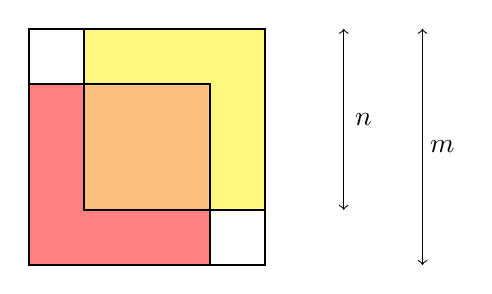
\begin{tikzpicture}
    \draw[thick] (0,0) rectangle (3,3);
    \draw[thick, fill=red!50] (0,0) rectangle (2.3,2.3);
    \draw[thick, fill=yellow!50] (0.7,0.7) rectangle (3, 3);
    \draw[thick, fill=orange!50] (0.7,0.7) rectangle (2.3, 2.3);
    \draw[<->] (4, 0.7)--(4, 3);
    \node at (4.25, 1.85) (n) {$n$};
    \draw[<->] (5, 0)--(5, 3);
    \node at (5.25, 1.5) (m) {$m$};
  \end{tikzpicture}
\end{center}
$m^2 = 2n^2$ હોવાથી $n$ બાજુવાળા બંને ચોરસો જ્યાં પરસ્પર આવરે છે
તે પ્રદેશનું ક્ષેત્રફળ બંને ચોરસોમાંથી કોઈ પણ ન આવરે એવા પ્રદેશના
ક્ષેત્રફળ જેટલું છે; એટલે કે નારંગી ચોરસનું ક્ષેત્રફળ છાયા વિનાના બે
ચોરસોનાં ક્ષેત્રફળોના સરવાળા જેટલું છે. તેથી નારંગી ચોરસની બાજુ $p$
અને છાયા વિનાના દરેક ચોરસની બાજુ $q$ હોય તો $p^2 = 2q^2$. પરંતુ હવે
$p < m$, $q < n$, $p, q \in \Nat$ સાથે
$\sqrt{2} = \nicefrac{p}{q}$. આ $m$ અને $n$ને શક્ય તેટલા નાના પસંદ
કર્યા હતા એ હકીકતનો વિરોધ કરે છે.

\emph{બીજી, ઔપચારિક રીતે.} $m^{2} = 2n^{2}$ હોવાથી $m$ યુગ્મ છે.
($x$ અયુગ્મ હોય તો $x^2$ અયુગ્મ છે તે બતાવવું સરળ છે.) તેથી કોઈ
$r \in \Nat$ માટે $m = 2r$. ફેરગોઠવણી કરતાં $2r^2 = n^2$,
એટલે $n$ પણ યુગ્મ છે. આથી $m$ અને $n$ બંને યુગ્મ છે અને તેથી
$\nicefrac{m}{n}$ અપૂર્ણાંકને \emph{વધુ} સાદો કરી શકાય છે.
વિરોધાભાસ!
\end{proof}

પ્રસંગોપાત, આ આકૃતિમય સાબિતી આપણને \olref[his][set][mythology]{sec}ની
સામગ્રી ફરી વિચારવા દે છે. ટેનેનબાઉમ (1927--2006) પૂરેપૂરા આધુનિક
ગણિતજ્ઞ હતા; છતાં આ સાબિતી નિર્વિવાદપણે સુંદર, સંપૂર્ણ ચુસ્ત અને
ભૌમિતિક અંતઃપ્રજ્ઞા પર આધારિત છે!

કોઈ પણ રીતે જુઓ તો વાસ્તવિક સંખ્યાઓ સંમેય સંખ્યાઓ કરતાં ``વધુ
વિસ્તૃત'' છે. એક અર્થમાં સંમેય સંખ્યાઓમાં ``ખાલી જગ્યાઓ'' છે અને
વાસ્તવિક સંખ્યાઓ તે ભરે છે. વાયર્સ્ટ્રાસે સમજ્યું કે આ વાત વાસ્તવિક
સંખ્યાઓનો એક જ એવો ગુણધર્મ વર્ણવે છે જે તેમને સંમેય સંખ્યાઓથી જુદી
પાડે છે—એટલે પૂર્ણતા ગુણધર્મ: \emph{ઉચ્ચસીમા ધરાવતા વાસ્તવિક
સંખ્યાઓના દરેક અખાલી ગણને ન્યૂનતમ ઉચ્ચસીમા હોય છે.}

સંમેય સંખ્યાઓ પૂર્ણતા ગુણધર્મ ધરાવતી નથી તે સહેલાઈથી જોઈ શકાય છે.
દાખલા તરીકે $\sqrt{2}$ કરતાં નાની સંમેય સંખ્યાઓનો ગણ વિચારો, એટલે કે:
\[
  \Setabs{p \in \Rat}{p^2 < 2 \text{ અથવા }p < 0}
\]
આ ગણને સંમેય સંખ્યાઓમાં ઉચ્ચસીમા છે; દાખલા તરીકે તેના ઘટકો<
બધા $3$ કરતાં નાના છે. પરંતુ તેની ન્યૂનતમ ઉચ્ચસીમા શી છે? આપણે
`$\sqrt{2}$' કહેવા ઇચ્છીએ; પરંતુ હમણાં જ જોયું કે $\sqrt{2}$
\emph{સંમેય નથી}. અને $\sqrt{2}$ કરતાં મોટી કોઈ \emph{ન્યૂનતમ}
સંમેય સંખ્યા નથી. તેથી આ ગણને ઉચ્ચસીમા છે પરંતુ ન્યૂનતમ ઉચ્ચસીમા નથી.
પરિણામે સંમેય સંખ્યાઓ પૂર્ણતા ગુણધર્મ ધરાવતી નથી.

તેનાથી વિપરીત, સાતત્યક ``તાત્ત્વિક રીતે'' પૂર્ણતા ગુણધર્મ ધરાવવું
જોઈએ. આપણે માત્ર $\sqrt{2}$ને વાસ્તવિક સંખ્યા બનાવવા નથી ઇચ્છતા;
સંમેય રેખાની બધી ``ખાલી જગ્યાઓ'' ભરવા ઇચ્છીએ છીએ. ખરેખર, સાતત્યકમાં
પોતે કોઈ ``ખાલી જગ્યા'' ન રહે એવું ઇચ્છીએ છીએ. પૂર્ણતા વડે આપણને
બરાબર આ જ મળશે.
% END OLP-0044
\endgroup

\begingroup
\makeatletter\def\ol@sectioncs{section}\makeatother

% BEGIN OLP-0045
\olfileid{sfr}{arith}{cuts}
\olsection{$\Rat$થી $\Real$ સુધી}
\phantomsection\label{guunit:OLP-0045}


મૂળ વાત એ છે કે પૂર્ણતા ગુણધર્મ બતાવે છે કે વાસ્તવિક રેખાનું કોઈ પણ
બિંદુ $\alpha$ એ રેખાને બે અર્ધભાગમાં બરાબર વહેંચે છે: એક ભાગ માટે
$\alpha$ ન્યૂનતમ ઉચ્ચસીમા છે અને બીજા માટે $\alpha$ મહત્તમ અધઃસીમા
છે. સંમેય સંખ્યાઓમાંથી વાસ્તવિક સંખ્યાઓની \emph{રચના} કરવા
ડેડેકિન્ડે સૂચવ્યું કે વાસ્તવિક સંખ્યાઓને સંમેય સંખ્યાઓનું વિભાજન કરતા
\emph{કાપ} તરીકે જ વિચારીએ. એટલે કે, $\sqrt{2}$ને એવા \emph{કાપ}
સાથે ઓળખીએ જે $< \sqrt{2}$ સંમેય સંખ્યાઓને $> \sqrt{2}$ સંમેય
સંખ્યાઓથી જુદી પાડે છે.

આ વિચારને સુઘડ બનાવીએ. સંમેય સંખ્યાઓને બે અર્ધભાગમાં કાપીએ તો કરેલા
વિભાજનને માત્ર તેના \emph{નીચલા} અર્ધભાગથી અનન્ય રીતે ઓળખી શકાય છે.
આથી ચોક્કસ વ્યાખ્યા નીચે મુજબ આપીએ છીએ:

\begin{defn}[કાપ]
\emph{કાપ} $\alpha$ એ સંમેય સંખ્યાઓનો એવો કોઈ પણ અખાલી ઉચિત
આરંભખંડ છે જેનો મહત્તમ ઘટક નથી. એટલે કે, $\alpha$ કાપ છે ત્યારે અને
માત્ર ત્યારે જ જ્યારે:
\begin{enumerate}
  \item \emph{અખાલી, ઉચિત}: $\emptyset \neq \alpha \subsetneq \Rat$
  \item \emph{આરંભિક}: બધા $p,q \in \Rat$ માટે, જો $p < q \in \alpha$ હોય તો $p \in \alpha$
  \item \emph{મહત્તમ ઘટક નહીં}: દરેક $p \in \alpha$ માટે કોઈ $q \in \alpha$ એવું છે કે $p < q$
\end{enumerate}
ત્યારે $\Real$ એ કાપોનો ગણ છે.
\end{defn}

હવે આપણે કહી શકીએ કે $\sqrt{2} = \Setabs{p \in \Rat}{p^2 < 2\text{
અથવા }p < 0}$. અલબત્ત, આ ખરેખર કાપ \emph{છે} તેની તપાસ કરવી પડે;
પરંતુ તે તપાસ \olref[check]{sec}માં રાખી છે.

પહેલાંની જેમ, કેટલીક વસ્તુઓની વ્યાખ્યા આપ્યા પછી હવે તેમના પરનાં
મૂળભૂત વિધેયો અને સંબંધોની વ્યાખ્યા કરવાની છે. એક સરળ વ્યાખ્યાથી શરૂ કરીએ:
\begin{align*}
  \alpha \leq \beta \text{ ત્યારે અને માત્ર ત્યારે જ જ્યારે }\alpha \subseteq \beta
\end{align*}
ક્રમની આ વ્યાખ્યા આપણને કેન્દ્રીય પરિણામ \emph{કહેવા} દે છે: કાપોનો
ગણ પૂર્ણતા ગુણધર્મ ધરાવે છે. પૂરેપૂરું લખીએ તો વિધાનનું સ્વરૂપ આવું છે.
$S$ એ ઉચ્ચસીમા ધરાવતો કાપોનો અખાલી ગણ હોય તો $S$ને ન્યૂનતમ ઉચ્ચસીમા
હોય છે. વધુ વિગતે: કોઈ કાપ $\lambda$ એ $S$ની ઉચ્ચસીમા છે, એટલે કે
$(\forall \alpha \in S)\alpha \subseteq \lambda$, અને $\lambda$ આવો
ન્યૂનતમ કાપ છે, એટલે કે
$(\forall \beta \in \Real)((\forall \alpha \in S)\alpha \subseteq \beta \lif \lambda \subseteq \beta)$.
હવે પરિણામની સાબિતી આ રહી:

\begin{thm}\ollabel{realcompleteness}
કાપોનો ગણ પૂર્ણતા ગુણધર્મ ધરાવે છે.
\end{thm}

\begin{proof}
$S$ એ ઉચ્ચસીમા ધરાવતો કાપોનો કોઈ અખાલી ગણ હોય. $\lambda = \bigcup S$ લો.
પહેલાં આપણે દાવો કરીએ કે $\lambda$ કાપ છે:
\begin{enumerate}
\item $S$ અખાલી હોવાથી ઓછામાં ઓછો એક કાપ $S$માં છે, તેથી
$\emptyset \neq \lambda$. $S$ કાપોનો ગણ હોવાથી $\lambda
\subseteq \Rat$. $S$ને ઉચ્ચસીમા હોવાથી કોઈ $p \in \Rat$ દરેક કાપ
$\alpha \in S$માંથી ગેરહાજર છે. તેથી $p\notin \lambda$, અને પરિણામે
$\lambda \subsetneq \Rat$.
\item ધારો કે $p < q \in \lambda$. ત્યારે કોઈ $\alpha \in S$ એવું
છે કે $q \in \alpha$. $\alpha$ કાપ હોવાથી $p \in \alpha$. તેથી
$p \in \lambda$.
\item ધારો કે $p \in \lambda$. ત્યારે કોઈ $\alpha \in S$ એવું છે કે
$p \in \alpha$. $\alpha$ કાપ હોવાથી કોઈ $q \in \alpha$ એવું છે કે
$p < q$. તેથી $q \in \lambda$.
\end{enumerate}
આથી દાવો સાબિત થયો. વધુમાં, સ્પષ્ટપણે $(\forall \alpha \in S)\alpha
\subseteq \bigcup S = \lambda$, એટલે કે $\lambda$ એ $S$ની ઉચ્ચસીમા
છે. હવે ધારો કે $\beta \in \mathbb{R}$ પણ ઉચ્ચસીમા છે, એટલે કે
$(\forall \alpha \in S)\alpha \subseteq \beta$. કોઈ પણ $p \in \Rat$
માટે, જો $p \in \lambda$ હોય તો કોઈ $\alpha \in S$ માટે
$p \in \alpha$, તેથી $p \in \beta$. સામાન્યકરણ કરતાં
$\lambda \subseteq \beta$. આથી $\lambda$ એ $S$ની \emph{ન્યૂનતમ}
ઉચ્ચસીમા છે.
\sourcecorrection{OLARI-002}{મૂળની \texttt{cuts.tex}, પંક્તિઓ 61--65માં
\(S\)માં ઓછામાં ઓછો એક કાપ હોવાનો આધાર ભૂલથી “\(S\)ને ઉચ્ચસીમા છે”
એમ આપ્યો છે. આ તારણ \(S\) અખાલી છે એ ધારણાથી મળે છે; અહીં તે જ
યોગ્ય ધારણા લખી છે.}
\end{proof}

આ રીતે આપણને પૂર્ણતા ગુણધર્મ ધરાવતી ઘણી વસ્તુઓ મળી છે. આને કહેવાની
એક રીત એ છે કે આપણા કાપોમાં કોઈ ``ખાલી જગ્યા'' નથી. (આથી સંમેય
સંખ્યાઓને બદલે વાસ્તવિક સંખ્યાઓના વધુ ``કાપ'' લેવાથી કોઈ રસપ્રદ નવી
વસ્તુઓ નહીં મળે.)

હવે વાસ્તવિક સંખ્યાઓ પર કેટલીક ક્રિયાઓ વ્યાખ્યાયિત કરવી પડશે.
દરેક $p \in \Rat$ માટે $p_\Real = \Setabs{q \in \Rat}{q < p}$ એમ
ઠરાવીને આપણે પહેલાં સંમેય સંખ્યાઓને વાસ્તવિક સંખ્યાઓમાં સ્થાપિત કરીએ છીએ.
પછી વ્યાખ્યા કરીએ છીએ:
\begin{align*}
  \alpha + \beta &= \Setabs{p + q}{p \in \alpha \land q \in \beta}\\
  \alpha \times \beta &=
  \Setabs{p \times q}{0 \leq p \in \alpha \land 0 \leq q \in \beta} \cup 0^\mathbb{R} & \text{ જો }\alpha, \beta \geq 0_\Real
\end{align*}
ગુણાકારના બીજા કિસ્સા સંભાળવા પહેલાં નીચે મુજબ લો: %કે $0_\Real \times \alpha = 0_\Real = \alpha \times 0_\Real$, અને ઉમેરો:
\begin{align*}
  -\alpha &= \Setabs{p - q}{p < 0 \land q \notin \alpha}
\end{align*}
અને પછી એમ ઠરાવો કે:
\begin{align*}
  \alpha \times \beta &\defis
  \begin{cases}
    \mathord{-}\alpha \times \mathord{-}\beta &\text{ જો }\alpha < 0_\Real\text{ અને }\beta < 0_\Real\\
    \mathord{-}(\mathord{-}\alpha \times \beta) &\text{ જો }\alpha < 0_\Real \text{ અને }\beta > 0_\Real\\
    \mathord{-}(\alpha \times \mathord{-}\beta) &\text{ જો }\alpha > 0_\Real \text{ અને }\beta < 0_\Real
  \end{cases}
\end{align*}
આમાંની દરેક વ્યાખ્યા હંમેશાં કાપ જ આપે છે તેની તપાસ કરવી પડશે.
છેલ્લે, આ રીતે વ્યાખ્યાયિત કાપોનો વ્યવહાર બરાબર જેવો હોવો જોઈએ
તેવો જ છે તેનું સરળ પરંતુ લાંબું નિદર્શન કરવું પડશે. આ બધું
\olref[check]{sec}માં રાખીએ છીએ.
% END OLP-0045
\endgroup

\begingroup
\makeatletter\def\ol@sectioncs{section}\makeatother

% BEGIN OLP-0046
\olfileid{sfr}{arith}{ref}
\olsection{કેટલાક તાત્ત્વિક પ્રતિચિંતનો}
\phantomsection\label{guunit:OLP-0046}


પ્રાવિધિક વિગતો આટલી થઈ. પરંતુ તેનાથી સિદ્ધ શું થયું?

એવું લગભગ નિર્વિવાદ છે કે તેનાથી આપણને થોડું {સુંદર} શુદ્ધ ગણિત
મળ્યું. ઉપરાંત કેટલીક ગહન વૈચારિક સિદ્ધિઓ મળી. પૂર્ણતા ગુણધર્મ
વાસ્તવિક અને સંમેય સંખ્યાઓ વચ્ચેનો નિર્ણાયક તફાવત વ્યક્ત કરે છે એવું
જોવું એક ગહન અંતર્દૃષ્ટિ હતું. વધુમાં, ડેડેકિન્ડ કાપ તરીકે વાસ્તવિક
સંખ્યાઓની સ્પષ્ટ રચના વિશ્લેષણના વિષયને મજબૂત પાયો આપે છે. કાપો
\emph{પૂર્ણ ક્રમિત ક્ષેત્ર} બનાવે છે, તેથી આ ખ્યાલ સુસંગત છે તે આપણે જાણીએ છીએ.

આ બધું સ્વીકાર્યા પછી પણ આ સિદ્ધિઓ વિશે કેટલીક શંકાઓ જણાવવી જોઈએ.

પહેલી વાત, વાસ્તવિક સંખ્યાઓને કાપો તરીકે વિચારવી એ તેમના પરિચિત
(કદાચ અનંત) દશાંશ વિસ્તરણોના રૂપમાં વિચારવા કરતાં \emph{વધુ} ચુસ્ત
છે કે નહીં તે સ્પષ્ટ નથી. વાસ્તવિક સંખ્યાઓની આ બીજી ``રચના'' કોશી
શ્રેણી વડે થતી રચના સાથે થોડું સામ્ય ધરાવે છે; પરંતુ હકીકતમાં
સત્તરમી સદીના આરંભથી ગણિતજ્ઞો તેને મૂળભૂત રીતે જાણતા હતા
(\olref[cauchy]{sec} જુઓ). ચુસ્તતામાં ખરેખરનો વધારો વાસ્તવિક સંખ્યાઓ
પૂર્ણતા ગુણધર્મ ધરાવે છે એ સમજવાથી થયો. ચોક્કસ ગણો તરીકે વાસ્તવિક
સંખ્યાઓ રચવાની ક્ષમતા કદાચ પોતાની રીતે એટલી રસપ્રદ નથી.

પૂર્ણાંકોનું કે સંમેય સંખ્યાઓનું (ઘણું સરળ) અંકગણિતીકરણ તે ક્ષેત્રોમાં
ચુસ્તતા વધારે છે કે નહીં તે તો હજી ઓછું સ્પષ્ટ છે. અહીં એક સરળ અવલોકન
ઉપયોગી છે. પ્રાકૃતિક સંખ્યાઓની ક્રમયુક્ત જોડોના સામ્ય વર્ગો તરીકે
પૂર્ણાંકોની \emph{રચના} કર્યા પછી, પૂર્ણાંકોની ક્રમયુક્ત જોડોના સામ્ય
વર્ગો તરીકે સંમેય સંખ્યાઓની રચના કર્યા પછી અને સંમેય સંખ્યાઓના ગણો
તરીકે વાસ્તવિક સંખ્યાઓ રચ્યા પછી આપણે તરત જ એ રચનાઓને \emph{ભૂલી
જઈએ છીએ}. ખાસ કરીને, ગણિતીય સાબિતીમાં કોઈ આ રચનાઓને ક્યારેય
\emph{ઉપયોગમાં લેવા} ઇચ્છશે નહીં (અલબત્ત, રચનાઓનો વ્યવહાર ધાર્યા મુજબ
છે એવી સાબિતી સિવાય). પ્રાકૃતિક સંખ્યાઓના ગણોના ગણોના ગણોના ગણોના
ગણોના ગણોના કોઈ ગણ વિશે બોલવા કરતાં સીધું કોઈ વાસ્તવિક સંખ્યા વિશે
બોલવું ઘણું સરળ છે.

આ વ્યાખ્યાઓ આપણને પૂર્ણાંકો, સંમેય સંખ્યાઓ કે વાસ્તવિક સંખ્યાઓ
\emph{અધિભૌતિક અર્થમાં શું છે} તે કહે છે એવો દાવો સૌથી વધુ
શંકાસ્પદ છે. એટલે કે, વાસ્તવિક સંખ્યાઓ (ધારો કે) ચોક્કસ ગણો
(ગણોના ગણોના ગણો\ldots) જ \emph{છે} એ શંકાસ્પદ છે. આવા મતનો મુખ્ય
અવરોધ એ છે કે રચના ઘણી જુદી રીતે થઈ શકી હોત. વાસ્તવિક સંખ્યાઓના
કિસ્સામાં ખરેખર રસપ્રદ રીતે જુદી રચનાઓ છે (\olref[cauchy]{sec} જુઓ).
પરંતુ તદ્દન જુદી રચનાઓ મેળવવાની આ એક નજીવી રીત છે: જેમ
\olref[sfr][rel][ref]{sec}માં જોયું, ક્રમયુક્ત જોડની વ્યાખ્યા સહેજ જુદી
રીતે કરી શકાઈ હોત; આ વૈકલ્પિક ખ્યાલ વાપર્યો હોત તો આપણી રચનાઓ એટલી
જ સારી રીતે કામ કરત, પરંતુ અંતે મળતી વસ્તુઓ જુદી હોત. આમ પૂર્ણાંકો,
સંમેય સંખ્યાઓ અને વાસ્તવિક સંખ્યાઓની ઘણી હરીફ ગણસૈદ્ધાંતિક રચનાઓ છે.
હવે પૂર્ણાંકો (ધારો કે) \emph{આ} ગણો છે, \emph{તે} નહીં, એવો દાવો
મનસ્વી (અને મૂંઝવણજનક) થશે. (\olref[sfr][rel][ref]{sec}ની જેમ આ પણ
\citealt{Benacerraf1965}એ પ્રસિદ્ધ કરેલી દલીલનું એક દૃષ્ટાંત છે.)

બીજો મુદ્દો પણ ઉઠાવવો જોઈએ: આપણી રચનાઓમાં કશુંક બહુ \emph{વિચિત્ર}
છે. આપણે પ્રાકૃતિક સંખ્યાઓથી શરૂ કર્યું. પછી પૂર્ણાંકો રચ્યા અને
``પૂર્ણાંકોનું $0$'', એટલે કે $\equivrep{0,0}{\Intequiv}$ રચ્યું.
પરંતુ $0 \neq \equivrep{0,0}{\Intequiv}$. ખરેખર, આપણી રચનાઓ મુજબ
\emph{કોઈ પણ} પ્રાકૃતિક સંખ્યા પૂર્ણાંક નથી. આ ખૂબ જ પ્રતિઅંતઃપ્રજ્ઞ
લાગે છે. વળી \olref[sfr][set][imp]{sec}માં આપણે બહુ દલીલ કર્યા વિના
$\Nat \subseteq \Rat$ એવો દાવો કર્યો હતો. જો આ રચનાઓ સંખ્યાઓ
\emph{બરાબર શું છે} તે કહેતી હોય, તો એ દાવો સહેજે ખોટો હતો.

હવે થોડું દૂરથી જોઈએ તો આપણે ક્યાં પહોંચ્યા? સહજ ગણસિદ્ધાંતમાં કામ
કરીને અને પ્રાકૃતિક સંખ્યાઓને આપેલી માનીને, પૂર્ણાંકો, સંમેય સંખ્યાઓ
અને વાસ્તવિક સંખ્યાઓને ચોક્કસ ગણો \emph{તરીકે} ગણી શકીએ છીએ. આ અર્થમાં
આ વસ્તુઓના સિદ્ધાંતોને ગણસિદ્ધાંતમાં \emph{સ્થાપિત} કરી શકીએ છીએ.
પરંતુ આ સ્થાપનનું તાત્ત્વિક મહત્ત્વ એટલું સીધું નથી.

અલબત્ત, આમાંથી કંઈ અંતિમ શબ્દ નથી!{} મુદ્દો માત્ર આ છે: વાસ્તવિક
સંખ્યાઓનું અંકગણિતીકરણ ગહન તાત્ત્વિક મહત્ત્વ \emph{ધરાવે છે} એવું
બતાવવા માટે કેટલીક વધારાની \emph{તાત્ત્વિક} દલીલ જરૂરી થશે.
% END OLP-0046
\endgroup

\begingroup
\makeatletter\def\ol@sectioncs{section}\makeatother

% BEGIN OLP-0047
\olfileid{sfr}{arith}{check}
\olsection{ક્રમિત મંડળો અને ક્ષેત્રો}
\phantomsection\label{guunit:OLP-0047}


આ આખા પ્રકરણમાં આપણે દાવો કર્યો કે અમુક વ્યાખ્યાઓનો વ્યવહાર
``જેવો હોવો જોઈએ તેવો'' છે. આ પ્રાવિધિક પરિશિષ્ટમાં તેનો અર્થ
સ્પષ્ટ કરીશું અને વ્યાખ્યાઓનો વ્યવહાર ``યોગ્ય રીતે'' થાય છે તે
(કેવી રીતે બતાવવું તેની રૂપરેખા) આપીશું.

\olref[int]{sec}માં આપણે $\Int$ પર સરવાળો અને ગુણાકાર વ્યાખ્યાયિત
કર્યા. વ્યાખ્યા મુજબ આ ક્રિયાઓ $\Int$ને આપણે ``ઇચ્છીએ તેવું''
સંરચના આપે છે એવું બતાવવું છે. ખાસ કરીને, અહીંની સંરચના સમક્રમી
મંડળની છે.

\begin{defn}
	\emph{સમક્રમી મંડળ} એવો ગણ $S$ છે જેમાં નિશ્ચિત ઘટકો $0$ અને $1$
	તથા ક્રિયાઓ $+$ અને $\times$ હોય અને જે નીચેના આઠ સૂત્રો સંતોષે:
	\begin{align*}
		\emph{સંગઠિતતા}&&a + (b+ c) & = (a + b) + c \\
		&& (a \times b) \times c & = a \times (b\times c)\\
		\emph{સમક્રમિતા}&&a + b &= b+ a  \\
		&&  a \times b&= b\times a\\
		\emph{એકમો}&&a + 0 &= a \\
		&& a \times 1 &= a\\
		\emph{યોજક વ્યસ્ત}&&(\exists b\in S)0&=a + b\\
		\emph{વિતરણાત્મકતા}&&a \times (b+ c ) &= (a \times b) + (a \times c)
	\end{align*}
	અહીં ગર્ભિત રીતે આ બધાં સૂત્રોના સર્વપરિમાણકો $S$ પૂરતા
	મર્યાદિત છે. એ પણ નોંધો કે અહીંના $0$ અને~$1$ નામના ઘટકો એ જ
	નામ ધરાવતી પ્રાકૃતિક સંખ્યાઓ હોવા જરૂરી નથી.
\end{defn}

તેથી પૂર્ણાંકો સમક્રમી મંડળ બનાવે છે કે નહીં તે ચકાસવા માટે આ આઠે
શરતો સંતોષાય છે એટલું જ ચકાસવાનું રહે છે. કોઈ શરત સ્થાપવી {મુશ્કેલ}
નથી, પણ એ કામ થોડું શ્રમસાધ્ય છે. દાખલા તરીકે, સરવાળાના કિસ્સામાં
\emph{સંગઠિતતા} આ રીતે સાબિત કરી શકાય:

\begin{proof}
$i, j, k \in \Int$ નિશ્ચિત કરો. ત્યારે એવા $a_1, b_1, a_2, b_2, a_3, b_3 \in
\Nat$ છે કે $i = \equivrep{a_1, b_1}{}$, $j =
\equivrep{a_2,b_2}{}$ અને $k = \equivrep{a_3, b_3}{}$. (વાંચવામાં
સરળતા રહે તે માટે આપણે ``$\equivrep{x, y}{\Intequiv}$''ને બદલે
``$\equivrep{x, y}{}$'' લખીએ છીએ; આ આખા વિભાગમાં એમ જ કરીશું.) હવે:
\begin{align*}
	i + (j + k) &= \equivrep{a_1, b_1}{}+(\equivrep{a_2, b_2}{} + \equivrep{a_3, b_3}{}) \\
	&= \equivrep{a_1,  b_1}{} + \equivrep{a_2+a_3, b_2+b_3}{}\\
	&= \equivrep{a_1 + (a_2 + a_3), b_1 + (b_2 + b_3)}{}\\
	&= \equivrep{(a_1 + a_2) + a_3, (b_1 + b_2) + b_3}{}\\
	&= \equivrep{a_1 + a_2, b_1 + b_2}{} + \equivrep{a_3, b_3}{}\\
	&= (\equivrep{a_1, b_1}{} + \equivrep{a_2, b_2}{}) + \equivrep{a_3, b_3}{}\\
	&= (i+j) + k
\end{align*}
અહીં $\Nat$ પરના સરવાળાના વ્યવહારનો આપણે નિઃસંકોચ ઉપયોગ કર્યો છે.
\end{proof}

એ જ રીતે \emph{યોજક વ્યસ્ત} આ રીતે સાબિત કરી શકાય:

\begin{proof}
$i \in \Int$ નિશ્ચિત કરો; ત્યારે કોઈ $a,b \in \Nat$ માટે $i =
\equivrep{a,b}{}$. $j = \equivrep{b,a}{} \in \Int$ લો. પ્રાકૃતિક
સંખ્યાઓના વ્યવહારનો ઉપયોગ કરતાં $(a+b) + 0 = 0 + (a+b)$, તેથી
વ્યાખ્યા મુજબ $\tuple{a+b, b+a} \sim_\Int \tuple{0,0}$, અને તેથી
$\equivrep{a+b, b+a}{} = \equivrep{0, 0}{} = 0_\Int$. હવે $i + j =
\equivrep{a,b}{}+\equivrep{b,a}{}=\equivrep{a+b, b+a}{}= \equivrep{0,
0}{} = 0_\Int$.
\end{proof}

અને \emph{વિતરણાત્મકતા}ની સાબિતી આ રહી:

\begin{proof}
ઉપરની જેમ $i = \equivrep{a_1, b_1}{}$, $j =
\equivrep{a_2,b_2}{}$ અને $k = \equivrep{a_3, b_3}{}$ નિશ્ચિત કરો. હવે:
\begin{align*}
	i \times (j + k)
	&= \equivrep{a_1, b_1}{} \times (\equivrep{a_2,b_2}{} + \equivrep{a_3, b_3}{})\\
	&= \equivrep{a_1, b_1}{} \times \equivrep{a_2 + a_3,b_2+b_3}{}\\
	&= \equivrep{a_1  (a_2 + a_3) + b_1  (b_2+b_3), a_1  (b_2 + b_3) + b_1 (a_2 + a_3)}{}\\
	&= \equivrep{a_1 a_2 + a_1a_3 + b_1 b_2+b_1b_3, a_1 b_2 + a_1b_3 + a_2b_1 + a_3b_1}{}\\
	&= \equivrep{a_1a_2 + b_1b_2, a_1b_2 + a_2b_1}{} + \equivrep{a_1a_3 + b_1b_3, a_1b_3 + a_3b_1}{}\\
	&= (\equivrep{a_1, b_1}{} \times \equivrep{a_2,b_2}{}) + (\equivrep{a_1, b_1}{} \times  \equivrep{a_3, b_3}{})\\
	&= (i \times j) + (i \times k)
\end{align*}
\end{proof}

બાકીની પાંચ શરતોની સાબિતી કસરત તરીકે છોડી દઈએ છીએ. એ કરી લઈએ
પછી આપણે બતાવ્યું હશે કે $\Int$ સમક્રમી મંડળ બનાવે છે, એટલે કે સરવાળો
અને ગુણાકારનો (વ્યાખ્યાયિત કરેલો) વ્યવહાર જેવો હોવો જોઈએ તેવો છે.

\begin{prob}
$\Int$ સમક્રમી મંડળ છે તે સાબિત કરો.
\end{prob}

પરંતુ આપણું કામ પૂરું થયું નથી. $\Int$ પર સરવાળો અને ગુણાકાર
વ્યાખ્યાયિત કરવા ઉપરાંત આપણે ક્રમસંબંધ $\leq$ પણ વ્યાખ્યાયિત કર્યો
હતો અને તેનો વ્યવહાર પણ જેવો હોવો જોઈએ તેવો છે એ ચકાસવું પડે. વધુ
ચોક્કસ રીતે, $\Int$ \emph{ક્રમિત} મંડળ બનાવે છે એવું બતાવવું પડશે.\footnote{
	\olref[sfr][rel][ord]{def:linearorder}માંથી યાદ કરો કે સંપૂર્ણ ક્રમ
	સ્વવાચક, પરંપરિત, વિસંમિત અને તુલનાયુક્ત સંબંધ છે. ક્રમસંબંધોના
	સંદર્ભમાં તુલનાયુક્તતાને ક્યારેક \emph{ત્રિવિકલ્પતા} કહે છે, કારણ કે
	કોઈ પણ $a$ અને $b$ માટે $a \leq b \lor a = b \lor a \geq b$.}

\begin{defn}
\emph{ક્રમિત મંડળ} એવું સમક્રમી મંડળ છે જેમાં સંપૂર્ણ ક્રમસંબંધ
$\leq$ પણ હોય અને નીચેની શરતો સંતોષાય:
\begin{align*}
	a \leq b &\lif a + c \leq b + c\\
	(a \leq b \land 0 \leq c) &\lif a \times c \leq b \times c
\end{align*}
\end{defn}

\begin{prob}
$\Int$ ક્રમિત મંડળ છે તે સાબિત કરો.
\end{prob}

અગાઉની જેમ રચાયેલું~$\Int$ ક્રમિત મંડળ છે એવું બતાવવું શ્રમસાધ્ય
પણ નિયમિત કામ છે. તે તમારા માટે છોડી દઈએ છીએ.

આમ પૂર્ણાંકોનું કામ પૂરું થયું. હવે સંમેય સંખ્યાઓ માટે આવી જ બાબતો
બતાવવી છે. ખાસ કરીને $+$, $\times$ અને $\leq$ની આપેલી વ્યાખ્યાઓ તળે
સંમેય સંખ્યાઓ ક્રમિત \emph{ક્ષેત્ર} બનાવે છે એવું બતાવવું છે:
\begin{defn}\ollabel{orderedfield}
\emph{ક્રમિત ક્ષેત્ર} એવું ક્રમિત મંડળ છે જે આ વધારાની શરત પણ સંતોષે:
\begin{align*}
	\emph{ગુણાકારી વ્યસ્ત}& & (\forall a \in S \setminus \{0\})(\exists b \in S) a\times b& = 1
\end{align*}
\end{defn}

$\Int$ ક્રમિત મંડળ બનાવે છે એવું બતાવી લીધા પછી $\Rat$ ક્રમિત ક્ષેત્ર
બનાવે છે એવું બતાવવું સરળ, પણ શ્રમસાધ્ય છે.

\begin{prob}
$\Rat$ ક્રમિત ક્ષેત્ર છે તે સાબિત કરો.
\end{prob}

પૂર્ણાંકો અને સંમેય સંખ્યાઓનું કામ પૂરું કર્યા પછી માત્ર વાસ્તવિક
સંખ્યાઓ બાકી રહે છે. ખાસ કરીને, $\Real$ \emph{પૂર્ણ} ક્રમિત ક્ષેત્ર,
એટલે કે પૂર્ણતા ગુણધર્મ ધરાવતું ક્રમિત ક્ષેત્ર, બનાવે છે એવું બતાવવું
પડે. \olref[cuts]{realcompleteness}માં $\Real$ પૂર્ણતા ગુણધર્મ ધરાવે
છે એવું સ્થાપ્યું હતું. પરંતુ $\Real$ ક્રમિત ક્ષેત્ર છે તેની
(કંટાળાજનક) ચકાસણીની વિગતો હજી બાકી છે.

આ શ્રમસાધ્ય કસરત તરફ વળતાં પહેલાં થોડી વધુ ``તાત્કાલિક'' બાબતો
ચકાસવી પડશે. દાખલા તરીકે, કોઈ પણ કાપો $\alpha$ અને $\beta$ માટે
વ્યાખ્યાયિત કરેલો $\alpha + \beta$ ખરેખર \emph{કાપ} જ છે તેની ખાતરી
કરવી પડશે. તેની સાબિતી આ રહી:

\begin{proof}
$\alpha$ અને $\beta$ બંને કાપ હોવાથી $\alpha + \beta = \Setabs{p
+ q}{p \in \alpha \land q \in \beta}$ એ $\Rat$નો અરિક્ત ઉચિત ઉપગણ
છે. હવે કોઈ $p \in \alpha$ અને $q \in \beta$ માટે $x < p + q$ ધારો.
ત્યારે $x - p < q$, તેથી $x - p \in \beta$, અને $x = p + (x - p) \in
\alpha + \beta$. તેથી $\alpha + \beta$ એ $\Rat$નો આરંભિક ખંડ છે.
અંતે, કોઈ પણ $p + q \in \alpha + \beta$ માટે, $\alpha$ અને $\beta$
બંને કાપ હોવાથી એવા $p_1 \in \alpha$ અને $q_1 \in \beta$ છે કે
$p < p_1$ અને $q < q_1$; તેથી $p + q < p_1 + q_1 \in \alpha +
\beta$; આમ $\alpha + \beta$ને કોઈ મહત્તમ ઘટક નથી.
\end{proof}

આવી જ મહેનતથી તમે ચકાસી શકશો કે $\alpha - \beta$, $\alpha \times
\beta$ અને $\alpha \div \beta$ પણ કાપ છે (છેલ્લા કિસ્સામાં $\beta$
શૂન્ય-કાપ હોય તે કિસ્સો અવગણવો). એ પણ આપણે તમારા માટે જ છોડી દઈએ છીએ.

\begin{prob}
$\Real$ ક્રમિત ક્ષેત્ર છે તે સાબિત કરો.
\end{prob}

હવે એક નાની અધૂરી વિગત પૂરી કરીએ. \olref[cuts]{sec}માં આપણે સૂચવ્યું
હતું કે $\sqrt{2} = \Setabs{p \in \Rat}{p < 0 \text{ અથવા }p^2 < 2}$
લઈ શકાય. પરંતુ આ ગણ \emph{કાપ} છે એવું બતાવવું પડે. તેની સાબિતી આ રહી:

\begin{proof}
સ્પષ્ટપણે આ સંમેય સંખ્યાઓનો અરિક્ત ઉચિત આરંભિક ખંડ છે; તેથી તેને
મહત્તમ ઘટક નથી એટલું બતાવવું પૂરતું છે. ખાસ કરીને, $p^2 < 2$ ધરાવતી
ધન સંમેય સંખ્યા $p$ અને $q = \frac{2p+2}{p+2}$ હોય ત્યારે $p < q$ અને
$q^2 < 2$ બંને બતાવવાં પૂરતાં છે. $p < q$ જોવા માટે માત્ર નોંધો:
\begin{align*}
	p^2 &< 2\\
	p^2 + 2p &< 2 + 2p\\
	p(p + 2) &< 2 + 2p\\
	p &< \tfrac{2+2p}{p+2} = q
\end{align*}
$q^2 < 2$ જોવા માટે માત્ર નોંધો:
\begin{align*}
	p^2 &< 2\\
	2p^2 + 4p + 2 &< p^2 + 4p+ 4\\
	4p^2 + 8p + 4 &< 2(p^2 + 4p + 4)\\
	(2p+2)^2 & <2(p+2)^2\\
	\tfrac{(2p+2)^2}{(p+2)^2} &< 2\\
	q^2 &< 2
\end{align*}
\end{proof}
% END OLP-0047
\endgroup

\begingroup
\makeatletter\def\ol@sectioncs{section}\makeatother

% BEGIN OLP-0048
\olfileid{sfr}{arith}{cauchy}

\olsection{પરિશિષ્ટ: કોશી શ્રેણીઓ તરીકે વાસ્તવિક સંખ્યાઓ}
\phantomsection\label{guunit:OLP-0048}


\olref[cuts]{sec}માં આપણે વાસ્તવિક સંખ્યાઓની રચના ડેડેકિન્ડ કાપો
તરીકે કરી. આ વિભાગમાં એક વૈકલ્પિક રચના સમજાવીશું. તે કોશીએ
(જેને હવે આપણે કોશી શ્રેણી કહીએ છીએ તેની) આપેલી વ્યાખ્યા પર આધારિત
છે; પરંતુ આ વ્યાખ્યાનો ઉપયોગ કરીને વાસ્તવિક સંખ્યાઓની \emph{રચના}
કરવાનું શ્રેય ઓગણીસમી સદીના બીજા લેખકોને, ખાસ કરીને વાયરસ્ટ્રાસ,
હાઇને, મેરે અને કૅન્ટૉરને જાય છે. (સરસ ઇતિહાસ માટે
\citeauthor{OConnorRobertson:RN} \citeyear{OConnorRobertson:RN} જુઓ.)

ઓગણીસમી સદી સુધી પહોંચતાં પહેલાં સિમોન સ્ટેવિન (1548--1620)નો વિચાર
કરવો યોગ્ય છે. ટૂંકમાં, સ્ટેવિને સમજ્યું કે દરેક વાસ્તવિક સંખ્યાને
તેના દશાંશ વિસ્તરણ દ્વારા વિચારી શકાય. તેથી $\sqrt{2}$ જેવી અસંમેય
સંખ્યાનું પણ સરસ દશાંશ વિસ્તરણ છે, જે આ રીતે શરૂ થાય છે:
\[
	1.41421356237\ldots
\]
ગણસિદ્ધાંતમાં દશાંશ વિસ્તરણોના પ્રતિરૂપ બનાવવા બહુ સરળ છે: તેમને
$d \colon \Nat \to \Nat$ વિધેયો તરીકે વિચારો, જ્યાં $d(n)$ આપણને
રસ હોય તે $n$મું દશાંશ સ્થાન છે. પછી દશાંશ ચિહ્નની પહેલાં આવતા
વાસ્તવિક સંખ્યાના ભાગને (અહીં માત્ર $1$ને) સંભાળવા વ્યાખ્યામાં થોડો
ફેરફાર કરવો પડશે. દાખલા તરીકે $0.999\ldots = 1$ની ખાતરી કરવા માટે
બીજો ફેરફાર (એક સામ્ય સંબંધ) પણ કરવો પડશે. પરંતુ સ્ટેવિનની રીત મુજબ
ગણસિદ્ધાંતમાં વાસ્તવિક સંખ્યાઓની પૂરેપૂરી ચુસ્ત રચના આપવી મુશ્કેલ નથી.

અહીં સ્ટેવિન આપણો મુખ્ય વિષય નથી. (સ્ટેવિન વિશે વધુ માટે
\citealt{KatzKatz2012} જુઓ.) પરંતુ આ રહ્યો તેની નજીકનો એક વિચાર.
$\sqrt{2}$ના દશાંશ વિસ્તરણને સીધું લેવાને બદલે વધુ ને વધુ ચોક્કસ
વિસ્તરણો લઈને $\sqrt{2}$નાં વધુ ને વધુ ચોક્કસ સંમેય આસન્ન મૂલ્યોની
એક \emph{શ્રેણી} વિચારી શકાય:
\[
1, 1.4, 1.414, 1.4142, 1.41421,\ldots
\]
વાસ્તવિક સંખ્યાઓને ``વધુ ને વધુ સારા આસન્ન મૂલ્યો'' દ્વારા વિચારી
શકાય એ વિચાર આપણને અંતર્દૃષ્ટિઓના બીજા ક્રમનો આધાર આપે છે (જેમ
$\Int$માંથી $\Rat$ અથવા $\Nat$માંથી $\Int$ રચતી વખતે મળેલી
અંતર્દૃષ્ટિઓ). મૂળભૂત અંતર્દૃષ્ટિઓ આ છે:
\begin{enumerate}
	\item દરેક વાસ્તવિક સંખ્યાને (કદાચ અનંત) દશાંશ વિસ્તરણ તરીકે લખી
	શકાય છે.
	\item (કદાચ અનંત) દશાંશ વિસ્તરણમાં સમાયેલી માહિતીને સંમેય સંખ્યાઓની
	શ્રેણીથી પણ એટલી જ રીતે રજૂ કરી શકાય છે.
	\item સંમેય સંખ્યાઓની શ્રેણીને $\Nat$માંથી $\Rat$માં જતા વિધેય
	તરીકે વિચારી શકાય; શ્રેણીની $n$મી સંમેય સંખ્યાને $f(n)$ લો.
\end{enumerate}
અલબત્ત, $\Nat$માંથી $\Rat$માં જતું \emph{કોઈ પણ} વિધેય આપણને વાસ્તવિક
સંખ્યા આપશે એવું નથી. દાખલા તરીકે, આ વિધેય વિચારો:
\[
	f(n) =\begin{cases}
			1 & \text{જો }n\text{ અયુગ્મ હોય}\\
			0 &\text{જો }n\text{ યુગ્મ હોય}
		\end{cases}
\]
અહીં મૂળ ચિંતા એ છે કે $0,1,0,1,0,1,0,\ldots$ શ્રેણી કોઈ વાસ્તવિક
સંખ્યા તરફ ``નજીક જતી'' જણાતી નથી. તેથી કોઈ વાસ્તવિક સંખ્યા તરફ
નજીક જતી શ્રેણીઓ જ વિચારવામાં આવે એની ખાતરી કરવા માટે આપણે કોઈ
\emph{લક્ષ} ધરાવતી શ્રેણીઓ પૂરતું ધ્યાન મર્યાદિત કરવું પડશે.

લક્ષનો વિચાર આપણે \olref[his][set][limits]{sec}માં જોઈ ચૂક્યા છીએ.
પરંતુ ત્યાં લીધેલી વ્યાખ્યા \emph{બરાબર} એ જ રીતે અહીં લઈ શકીએ નહીં.
ત્યાં ``$(\forall \epsilon>0)$'' અભિવ્યક્તિમાં વાસ્તવિક સંખ્યાઓ પરનું
પરિમાણીકરણ ગર્ભિત હતું; અને આપણે વાસ્તવિક સંખ્યાઓ પરનાં વિધેયોના
લક્ષ વિચારતા હતા. એટલે એ વ્યાખ્યાનો ઉપયોગ કરીએ તો જે વાસ્તવિક સંખ્યાઓની
\emph{રચના} કરવાનું આપણું લક્ષ છે તેને પહેલાંથી જ માની લઈએ. સદભાગ્યે,
લક્ષના અત્યંત નજીકના એક વિચારથી કામ ચાલી શકે છે.
\begin{defn}\ollabel{def:CauchySequence}
  વિધેય $f: \Nat \to \Rat$ \emph{કોશી શ્રેણી} હોય ત્યારે અને માત્ર
  ત્યારે જ જ્યારે દરેક ધન $\epsilon \in \Rat$ માટે $(\exists \ell \in
  \Nat)(\forall m, n > \ell)|f(m) - f(n)| < \epsilon$.
\end{defn}

લક્ષનો સામાન્ય વિચાર પહેલાં જેવો જ છે: તમને ($\epsilon$થી મપાતું)
અમુક ચોકસાઈનું સ્તર જોઈતું હોય તો જોવા માટે એક ``વિસ્તાર'' (એટલે કે
$\ell$ કરતાં મોટું કોઈ પણ આગત) મળે છે. આપણી શ્રેણી $1$, $1.4$,
$1.414$, $1.4142$, $1.41421$\ldots{}ને લક્ષ છે એવું જોવું પણ સરળ છે:
$\sqrt{2}$નું $\nicefrac{1}{10^{n}}$ જેટલી ત્રુટિની અંદર આસન્ન મૂલ્ય
જોઈતું હોય તો $n$મા ઘટક પછીના કોઈ પણ ઘટકને જુઓ.

ત્યારે પહેલો સ્વાભાવિક વિચાર એવો આવે કે કોઈ પણ કોશી શ્રેણી બસ એક
વાસ્તવિક સંખ્યા \emph{છે}. પરંતુ $\Int$ અને $\Rat$ની રચનાઓની જેમ આ
વિચાર બહુ ભોળો થશે: આપેલી કોઈ એક વાસ્તવિક સંખ્યાને ઘણી જુદી કોશી
શ્રેણીઓ સૂચવે છે. આ જોવાની એક સરળ રીત આ છે. કોશી શ્રેણી~$f$ આપેલી
હોય ત્યારે $g$ને $f$ જેવું જ વિધેય વ્યાખ્યાયિત કરો, માત્ર $g(0)\neq
f(0)$ રાખો. બંને શ્રેણીઓ પહેલા ઘટક પછી સર્વત્ર એકમત હોવાથી આપણે
(અંતે) એમ કહેવા ઇચ્છીશું કે \olref{def:CauchySequence}માં વપરાયેલા
અર્થમાં તેમને એક જ લક્ષ છે અને તેથી તેઓ એક જ વાસ્તવિક સંખ્યાને
``વ્યાખ્યાયિત'' કરે છે. તેથી આ કોશી શ્રેણીઓને ખરેખર એક જ વાસ્તવિક
સંખ્યા તરીકે વિચારવી જોઈએ.

આથી ફરી કોશી શ્રેણીઓ પર સામ્ય સંબંધ વ્યાખ્યાયિત કરીને વાસ્તવિક
સંખ્યાઓને સામ્ય \emph{વર્ગો} સાથે ઓળખવી પડશે. પહેલાં લક્ષમાં $0$
તરફ અભિસરતા વિધેયનો વિચાર જોઈએ. કોઈ પણ $h : \Nat \to \Rat$ માટે
કહો કે \emph{$h$ લક્ષમાં $0$ તરફ અભિસરે છે} ત્યારે અને માત્ર ત્યારે
જ્યારે દરેક ધન $\epsilon \in \Rat$ માટે $(\exists \ell \in
\Nat)(\forall n > \ell)|h(n)| < \epsilon$.\footnote{$\lim_{x
\mathord{\rightarrow}\infty}f(x) = 0$ની વ્યાખ્યા સાથે સરખાવો;
\olref[his][set][limits]{sec} જુઓ.} વધુમાં, $f$ અને $g$ એ
$\Nat \to \Rat$ વિધેયો હોય ત્યારે $(f-g)(n) = f(n) - g(n)$ લો. હવે
વ્યાખ્યા આપો:
\[
	f \Realequiv g \text{ ત્યારે અને માત્ર ત્યારે જ જ્યારે $(f-g)$ લક્ષમાં $0$ તરફ અભિસરે છે}.
\]
$\Realequiv$ સામ્ય સંબંધ છે એ ચકાસવું પડે; અને તે છે. પછી ઇચ્છીએ તો
વાસ્તવિક સંખ્યાઓને $\Nat \to \Rat$ જતી બધી કોશી શ્રેણીઓના
$\Realequiv$ તળેના સામ્ય વર્ગો તરીકે વ્યાખ્યાયિત કરી શકીએ.
\sourcecorrection{OLARI-003}{મૂળની \texttt{cauchy.tex}, પંક્તિઓ
84--93માં વાસ્તવિક સંખ્યાઓને સામ્ય \emph{સંબંધો} સાથે ઓળખવાનું કહેવાયું
છે, જોકે પછીનું વાક્ય યોગ્ય રીતે સામ્ય વર્ગો વાપરે છે. પંક્તિઓ
152--161નાં પ્રમેય અને પ્રશ્નમાં પણ શ્રેણીઓ કહેવાને બદલે એમના સામ્ય
વર્ગો અભિપ્રેત છે. અહીં ત્રણેય સ્થળે એ વર્ગો સ્પષ્ટ કર્યા છે.}

\begin{prob}
દરેક $n$ માટે $f(n) = 0$ લો. $g(n) = \frac{1}{(n+1)^2}$ લો. બંને
કોશી શ્રેણીઓ છે અને ખરેખર બંને વિધેયોનું લક્ષ $0$ છે, જેથી
$f \sim_\Real g$ પણ થાય છે, તે બતાવો.
\end{prob}

આ કરી લીધા પછી હંમેશની જેમ $f$ને ઘટક તરીકે ધરાવતા સામ્ય
વર્ગ માટે $\equivrep{f}{\Realequiv}$ લખીશું. પરંતુ વાંચવામાં સરળતા
રહે તે માટે હવે પછી નીચેનો સૂચક છોડીને માત્ર $\equivrep{f}{}$ લખીશું.
દરેક $q \in \Rat$ માટે $q_{\Real} = \equivrep{c_{q}}{}$ પણ ઠરાવીએ
છીએ, જ્યાં દરેક $n \in \Nat$ માટે $c_q(n) = q$ એવું અચળ વિધેય $c_{q}$
છે. પછી વાસ્તવિક સંખ્યાઓ પરના મૂળભૂત સંબંધો અને ક્રિયાઓ આ રીતે
વ્યાખ્યાયિત કરીએ છીએ:
\begin{align*}
	\equivrep{f}{} + \equivrep{g}{} &= 	\equivrep{(f + g)}{} \\
	\equivrep{f}{} \times 	\equivrep{g}{} &= \equivrep{(f \times g)}{}
\end{align*}
જ્યાં $(f + g)(n) = f(n) + g(n)$ અને $(f \times g)(n) = f(n) \times
g(n)$. અલબત્ત, $f$ અને $g$ કોશી શ્રેણીઓ હોય ત્યારે $(f + g)$,
$(f-g)$ અને $(f\times g)$માંનું દરેક કોશી શ્રેણી છે એ પણ ચકાસવું પડે;
તેઓ છે, અને એ કામ તમારા માટે છોડી દઈએ છીએ.

છેલ્લે, ક્રમનો ખ્યાલ વ્યાખ્યાયિત કરીએ. $\equivrep{f}{}$ને
\emph{ધન} કહો ત્યારે અને માત્ર ત્યારે જ જ્યારે $\equivrep{f}{}\neq
0_\Real$ અને $(\exists \ell \in \Nat)(\forall n > \ell)0 < f(n)$
બંને થાય. પછી $\equivrep{f}{} < \equivrep{g}{}$ ત્યારે અને માત્ર
ત્યારે જ જ્યારે $\equivrep{(g - f)}{}$ ધન હોય. આ સુવ્યાખ્યાયિત છે
(એટલે કે સામ્ય વર્ગમાંથી પસંદ કરેલા ``પ્રતિનિધિ'' વિધેય પર આધાર
રાખતું નથી) એ ચકાસવું પડશે.
\sourcecorrection{OLARI-004}{મૂળની \texttt{cauchy.tex}, પંક્તિઓ
137--139માં વાસ્તવિક સંખ્યાના સામ્ય વર્ગની ધનતા વ્યાખ્યાયિત કરતી
વખતે તેને સંમેય શૂન્ય \(0_\Rat\)થી જુદો કહ્યો છે. અહીં યોગ્ય પ્રકારનું
વાસ્તવિક શૂન્ય \(0_\Real\) વાપર્યું છે.}
પરંતુ આ ચકાસ્યા પછી આ વ્યાખ્યાઓ યોગ્ય બીજગાણિતિક ગુણધર્મો આપે છે
એ બતાવવું ઘણું સરળ છે; એટલે કે:
\begin{thm}\ollabel{thm:cauchyorderedfield}
કોશી શ્રેણીઓના સામ્ય વર્ગો ક્રમિત ક્ષેત્ર બનાવે છે.
\end{thm}

\begin{proof}
કસરત.
\end{proof}

\begin{prob}
કોશી શ્રેણીઓના સામ્ય વર્ગો ક્રમિત ક્ષેત્ર બનાવે છે તે સાબિત કરો.
\end{prob}

આ રીતે રચેલી વાસ્તવિક સંખ્યાઓ પૂર્ણતા ગુણધર્મ ધરાવે છે એવું સાબિત
કરવું વધુ મુશ્કેલ છે, તેથી આપણે તેની સાબિતી આપીશું.

\begin{thm}
ઉચ્ચસીમા ધરાવતા કોશી શ્રેણીઓના દરેક અરિક્ત ગણને ન્યૂનતમ ઉચ્ચસીમા છે.
\end{thm}

\begin{proof}[સાબિતીની રૂપરેખા] ઉચ્ચસીમા ધરાવતો કોશી શ્રેણીઓનો કોઈ
અરિક્ત ગણ $S$ લો. તેથી કોઈ $p \in \Rat$ એવો છે કે $p_{\Real}$ એ
$S$ની ઉચ્ચસીમા છે. $r \in S$ લો; ત્યારે કોઈ $q \in \Rat$ એવો છે
કે $q_{\Real} < r$. તેથી $S$ની ન્યૂનતમ ઉચ્ચસીમા અસ્તિત્વ ધરાવતી હોય
તો તે $q_\Real$ અને $p_\Real$ની વચ્ચે (અંતિમ મૂલ્યો સહિત) છે.

નીચેથી અને ઉપરથી એકસાથે નજીક જઈને આપણે ન્યૂનતમ ઉચ્ચસીમા તરફ
સંકુચિત થઈશું. ખાસ કરીને, $f$ ઉપરથી અને $g$ નીચેથી ન્યૂનતમ
ઉચ્ચસીમા તરફ સંકુચિત થાય એ હેતુથી બે વિધેયો $f, g \colon \Nat \to
\Rat$ વ્યાખ્યાયિત કરીએ છીએ. શરૂઆતમાં આ વ્યાખ્યાઓ આપીએ:
\begin{align*}
	f(0) &= p \\
	g(0) &= q
\end{align*}
પછી $a_n = \frac{f(n) + g(n)}{2}$ હોય ત્યારે લો:\footnote{આ
આવર્તક વ્યાખ્યા છે. પરંતુ આવર્તક વ્યાખ્યાઓ વાજબી છે એવું વિચારવાનું
કોઈ કારણ આપણે \emph{હજી} આપ્યું નથી.}
\begin{align*}
	f(n+1) &=
	\begin{cases}
		a_n &\text{જો }(\forall h \in S)\equivrep{h}{} \leq (a_n)_\Real\\
		f(n)&\text{અન્યથા}
	\end{cases}\\
	g(n+1) &=
	\begin{cases}
		a_n &\text{જો }(\exists h \in S)\equivrep{h}{} \geq (a_n)_\Real\\
		g(n) &\text{અન્યથા}
	\end{cases}
\end{align*}
$f$ અને $g$ બંને કોશી શ્રેણીઓ છે. (આ ચકાસવું ઘણું સરળ છે, પણ આપણે
તે કસરત તરીકે છોડીએ છીએ.) $(f-g)$ વિધેય લક્ષમાં $0$ તરફ અભિસરે છે,
કારણ કે દરેક પગલે $f$ અને $g$ વચ્ચેનો તફાવત અડધો થાય છે. તેથી
$\equivrep{f}{} = \equivrep{g}{}$.

પહેલાં બતાવીએ કે $\equivrep{f}{}$ એ $S$ની ઉચ્ચસીમા છે, એટલે કે
$(\forall h \in S)\equivrep{h}{} \leq \equivrep{f}{}$.
(આગળ વધતાં આપણે \olref{thm:cauchyorderedfield}નો ઉપયોગ કરીશું.)
$h \in S$ લો અને પ્રતિષેધ માટે ધારો કે $\equivrep{f}{} <
\equivrep{h}{}$, જેથી $0_\Real < \equivrep{(h-f)}{}$. $f$ એકધારી રીતે
ઘટતી કોશી શ્રેણી હોવાથી કોઈ $n \in \Nat$ એવો છે કે
$\equivrep{(c_{f(n)} - f)}{} < \equivrep{(h-f)}{}$. તેથી:
\[
	(f(n))_\Real = \equivrep{c_{f(n)}}{} < \equivrep{f}{} + \equivrep{(h-f)}{} = \equivrep{h}{},
\]
જે રચના મુજબ $\equivrep{h}{} \leq (f(n))_\Real$ હોવાનો વિરોધાભાસ છે.

હવે બતાવીએ કે $\equivrep{f}{} = \equivrep{g}{}$ એ $S$ની
\emph{ન્યૂનતમ} ઉચ્ચસીમા છે. કોઈ કોશી શ્રેણી $j$ લો અને ધારો કે
$\equivrep{j}{} < \equivrep{g}{}$. ઉપરની જેમ વિચારતાં ($g$
\emph{વધતી} છે એ હકીકતનો ઉપયોગ કરીને), કોઈ $n \in \Nat$ એવો છે કે
$\equivrep{j}{} < (g(n))_\Real$. પરંતુ રચના મુજબ કોઈ $h \in S$ એવો
છે કે $(g(n))_\Real \leq \equivrep{h}{}$, તેથી $\equivrep{j}{} <
\equivrep{h}{}$ અને એટલે $\equivrep{j}{}$ એ $S$ની ઉચ્ચસીમા નથી.
\end{proof}
% END OLP-0048
\endgroup


\OLEndChapterHook
% END OLP-0041
\endgroup


\begingroup
\makeatletter\def\ol@sectioncs{section}\makeatother

% BEGIN OLP-0049
\olchapter{sfr}{infinite}{અનંત ગણો}
\olchapterid{sfr}{infinite}
\phantomsection\label{guunit:OLP-0049}


\begin{editorial}
અનંત ગણો વિશેનું આ પ્રકરણ ટિમ બટનના \emph{Open Set Theory}માંથી
લેવામાં આવ્યું છે.
\end{editorial}

\begingroup
\makeatletter\def\ol@sectioncs{section}\makeatother

% BEGIN OLP-0050
\olfileid{sfr}{infinite}{hilbert}
\olsection{હિલ્બર્ટની હોટેલ}
\phantomsection\label{guunit:OLP-0050}


પ્રાકૃતિક સંખ્યાઓનો ગણ સ્પષ્ટપણે અનંત છે. તેથી, જો આપણે પ્રાકૃતિક
સંખ્યાઓને \emph{પહેલેથી જ માની લેવા} ન માગતા હોઈએ, તો આપણું પહેલું
પગલું પ્રાકૃતિક સંખ્યાઓનો પોતાનો ઉલ્લેખ કર્યા વિના અનંત ગણનું લક્ષણ
આપવાનું હોવું જોઈએ. ૧૯૨૪ના એક વ્યાખ્યાનમાં હિલ્બર્ટે રજૂ કરેલો આ એક
સુંદર અભિગમ છે. તેઓ આપણને કલ્પના કરવાનું કહે છે:
\begin{quote}
[\ldots] સાન્ત સંખ્યામાં ઓરડાઓ ધરાવતી એક હોટેલ. આ બધા ઓરડાઓમાં
બરાબર એક-એક મહેમાન રહેતો હોવો જોઈએ. હવે મહેમાનો કોઈક રીતે પોતાના
ઓરડા બદલે, [પણ] દરેક ઓરડામાં હજી વધુમાં વધુ એક જ વ્યક્તિ રહે એ રીતે,
તો એકેય ઓરડો ખાલી નહીં થાય અને હોટેલમાલિક આ રીતે નવા આવેલા મહેમાન
માટે નવી જગ્યા ઊભી કરી શકશે નહીં [\ldots
\textparagraph \ldots]

હવે આપણે ઠરાવીએ કે હોટેલમાં $1$, $2$, $3$, $4$, $5$, \dots એ રીતે
ક્રમાંકિત અનંત ઓરડાઓ હોય અને દરેકમાં બરાબર એક મહેમાન રહેતો હોય. નવો
મહેમાન આવે કે તરત માલિકે જૂના દરેક મહેમાનને તેના હાલના ક્રમાંક કરતાં
એક વધુ ક્રમાંકવાળા ઓરડામાં ખસેડવાનો જ રહે છે; ત્યારે નવા આવેલા મહેમાન
માટે ઓરડો~$1$ ખાલી થઈ જશે.
	\begin{center}
		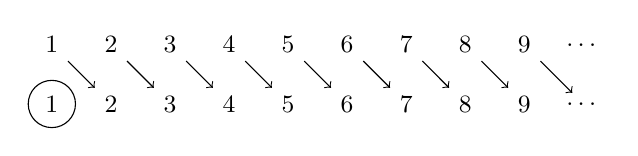
\begin{tikzpicture}[scale = .75]
		\foreach \x in {1, 2, 3, 4, 5, 6, 7, 8, 9}
		{
			\node (\x a) at (\x, 1) {\small{\x}};
			\node (\x b) at (\x, 2) {\small{\x}};
		}
		\node (dotsa) at (10, 1) {\small{\ldots}};
		\node (dotsb) at (10, 2) {\small{\ldots}};
		\draw[->] (1b)--(2a);
		\draw[->] (2b)--(3a);
		\draw[->] (3b)--(4a);
		\draw[->] (4b)--(5a);
		\draw[->] (5b)--(6a);
		\draw[->] (6b)--(7a);
		\draw[->] (7b)--(8a);
		\draw[->] (8b)--(9a);
		\draw[->] (9b)--(dotsa);
		\draw (1,1) circle (.4);
		\end{tikzpicture}
	\end{center}
	(\citealt[730]{EwaldSieg2013}માં પ્રકાશિત; અમારો અનુવાદ)
\end{quote}
નિર્ણાયક મુદ્દો એ છે કે હિલ્બર્ટની હોટેલમાં અનંત ઓરડાઓ છે; અને આમ
કહેવાનો અર્થ શું થાય તેની વ્યાખ્યા તરીકે આપણે તેમની સમજૂતી લઈ શકીએ.
ખરેખર, ડેડેકિન્ડનો અભિગમ પણ આ જ હતો (અલબત્ત, અહીં ભારે કાળવિપર્યય
સાથે રજૂ કર્યો છે; ડેડેકિન્ડની વ્યાખ્યા \citeyear{Dedekind1888}ની છે):

\begin{defn}\ollabel{defn:DedekindInfinite}
ગણ $A$ \emph{ડેડેકિન્ડ-અનંત} હોય જો અને માત્ર જો $A$થી $A$ના કોઈ
ઉચિત ઉપગણમાં એક-એક વિધેય હોય. એટલે કે, કોઈ $o \in A$ અને
એક-એક વિધેય $f \colon A \to A$ એવાં હોય કે $o \notin \ran{f}$.
\end{defn}
% END OLP-0050
\endgroup

\begingroup
\makeatletter\def\ol@sectioncs{section}\makeatother

% BEGIN OLP-0051
\olfileid{sfr}{infinite}{dedekind}
\olsection{ડેડેકિન્ડ બીજગણિતો}
\phantomsection\label{guunit:OLP-0051}


આપણે પ્રાકૃતિક સંખ્યાઓ માત્ર અનંત હોય એટલું જ નથી માગતા; આપણે એમ પણ
માગીએ છીએ કે તેમને અમુક (બૈજિક) ગુણધર્મો હોય: સરવાળા, ગુણાકાર વગેરે
હેઠળ તેમનો વ્યવહાર સુસંગત હોવો જોઈએ.

ડેડેકિન્ડનો વિચાર \emph{અનુગામી વિધેય}ના ખ્યાલને મૂળભૂત માનવાનો અને
પછી નીચેના ગુણધર્મો ધરાવતી સંખ્યાઓ તરીકે તેમનું લક્ષણ આપવાનો હતો:
\begin{enumerate}
	\item એવી સંખ્યા $0$ છે જે કોઈ પણ સંખ્યાની અનુગામી નથી
	\\અર્થાત્, $0 \notin \ran{s}$
	\\અર્થાત્, $\forall x\ s(x) \neq 0$
	\item ભિન્ન સંખ્યાઓના અનુગામીઓ ભિન્ન હોય છે
	\\અર્થાત્, $s$ એ એક-એક વિધેય છે
	\\અર્થાત્, $\forall x \forall y (s(x) = s(y) \lif x = y)$
	\item\ollabel{repeatedapplication} દરેક સંખ્યા $0$ પર અનુગામી
	વિધેય વારંવાર લગાડવાથી મળે છે.
\end{enumerate}
પહેલી બે શરતોને પ્રથમ-ક્રમ તર્કશાસ્ત્રથી સહેલાઈથી સંભાળી શકાય છે
(ઉપર જુઓ). પરંતુ માત્ર પ્રથમ-ક્રમ તર્કશાસ્ત્રથી
\olref{repeatedapplication}ને સંભાળી શકાતી નથી. ડેડેકિન્ડની સફળતા
શરત \olref{repeatedapplication}ને ગણસૈદ્ધાંતિક રીતે આ પ્રમાણે ફરી
ઘડવામાં હતી:
\begin{enumerate}
	\item[3$'$.] પ્રાકૃતિક સંખ્યાઓ એવો નાનામાં નાનો ગણ છે જે
	\emph{અનુગામી વિધેય હેઠળ સંવૃત} છે: એટલે કે, ગણના કોઈ પણ
	ઘટક પર $s$ લગાડીએ તો ગણનો બીજો ઘટક મળે છે.
\end{enumerate}
પરંતુ આ વાત આપણે ધીમે ધીમે પૂરેપૂરી સ્પષ્ટ કરવી પડશે.

\begin{defn}\ollabel{Closure}
	દરેક વિધેય $f \colon A \to A$ માટે ગણ $X \subseteq A$ એ
	$f$-\emph{સંવૃત} છે {iff} $(\forall x \in X)f(x) \in X$.
	હવે દરેક $o \in A$ માટે વ્યાખ્યા કરીએ:
	$$\closureofunder{f}{o} = \bigcap\Setabs{X}{o \in X\text{ અને }X
\text{ એ $f$-સંવૃત છે}}$$
\end{defn}
\sourcecorrection{OLINF-001}{મૂળની \texttt{dedekind-algebra.tex},
પંક્તિઓ 40--64માં સંવરણની વ્યાખ્યા કોઈ પણ $f$ અને $o$ માટે અપાઈ
છે, પછીના લેમામાં $A$ને બાંધ્યા વિના $o\in A$ લખાયું છે, અને
સાબિતીમાં $\ran{f}\cup\{o\}$ એ $f$-સંવૃત હોવાનો ઉપયોગ થાય છે.
આ દલીલને જરૂરી અને પછીના બધા ઉપયોગો સાથે સુસંગત એવી ધારણા
$f\colon A\to A$, $X\subseteq A$ અને $o\in A$ અહીં સ્પષ્ટ કરી છે.}

આમ $\closureofunder{f}{o}$ એ એવા બધા $f$-સંવૃત ગણોનો છેદ છે
જેમનો ઘટક~$o$ છે. તેથી સહજ રીતે,
$\closureofunder{f}{o}$ એ ઘટક તરીકે $o$ ધરાવતો
\emph{નાનામાં નાનો} $f$-સંવૃત ગણ છે. આગળનું પરિણામ આ સહજ વિચારને
ચોક્કસ બનાવે છે;
\begin{lem}\ollabel{closureproperties}
	દરેક વિધેય $f \colon A \to A$ અને દરેક $o \in A$ માટે:
	\begin{enumerate}
		\item\ollabel{closurehaselem} $o \in \closureofunder{f}{o}$; અને
		\item\ollabel{closureclosed} $\closureofunder{f}{o}$ એ $f$-સંવૃત છે; અને
		\item\ollabel{closuresmallest} જો $X$ એ $f$-સંવૃત હોય અને $o \in
		X$, તો $\closureofunder{f}{o} \subseteq X$.
	\end{enumerate}
\end{lem}

\begin{proof}
નોંધો કે ઘટક તરીકે $o$ ધરાવતો ઓછામાં ઓછો એક $f$-સંવૃત ગણ
છે, એટલે કે $\ran{f}\cup \{o\}$. તેથી આવા \emph{બધા} ગણોનો છેદ
$\closureofunder{f}{o}$ અસ્તિત્વ ધરાવે છે. હવે આપણે
\olref{closurehaselem}--\olref{closuresmallest} તપાસવાં છે.

\olref{closurehaselem} અંગે: $o \in \closureofunder{f}{o}$, કારણ કે
તે એવા ગણોનો છેદ છે જેમના દરેકનો ઘટક~$o$ છે.

\olref{closureclosed} અંગે: ધારો કે $x \in \closureofunder{f}{o}$.
તેથી જો $o \in X$ અને $X$ એ $f$-સંવૃત હોય, તો $x \in X$; અને
$X$ એ $f$-સંવૃત હોવાથી હવે $f(x) \in X$. તેથી
$f(x) \in \closureofunder{f}{o}$.

\olref{closuresmallest} અંગે: સામાન્ય રીતે, જો $X \in C$ હોય, તો
$\bigcap C \subseteq X$.
\end{proof}

આનો ઉપયોગ કરીને આપણે કહી શકીએ:

\begin{defn}
\emph{ડેડેકિન્ડ બીજગણિત} એટલે ગણ $A$, વિધેય $f \colon A \to A$
અને કોઈ $o \in A$ એવાં કે:
	\begin{enumerate}
		\item \ollabel{ded:proper} $o \notin \ran{f}$
		\item \ollabel{ded:injection} $f$ એ એક-એક વિધેય છે
		\item \ollabel{ded:closure} $A = \closureofunder{f}{o}$
	\end{enumerate}
\end{defn}

$A = \closureofunder{f}{o}$ હોવાથી આપણું પહેલાનું પરિણામ જણાવે છે કે
$A$ એ ઘટક તરીકે $o$ ધરાવતો નાનામાં નાનો $f$-સંવૃત ગણ છે.
ડેડેકિન્ડ બીજગણિત સ્પષ્ટપણે ડેડેકિન્ડ-અનંત છે; વ્યાખ્યાની કલમો
\olref{ded:proper} અને \olref{ded:injection} જ જુઓ. પરંતુ વધુ રસપ્રદ
હકીકત એ છે કે કોઈ પણ ડેડેકિન્ડ-અનંત ગણને ડેડેકિન્ડ બીજગણિતમાં ફેરવી
શકાય છે.

\begin{thm}\ollabel{thm:DedekindInfiniteAlgebra}
જો કોઈ ડેડેકિન્ડ-અનંત ગણ હોય, તો કોઈ ડેડેકિન્ડ બીજગણિત હોય છે.
\end{thm}

\begin{proof}
ધારો કે $D$ ડેડેકિન્ડ-અનંત છે. તેથી એક-એક વિધેય $g \colon D \to
D$ અને ઘટક $o \in D \setminus \ran{g}$ છે. હવે $A =
\closureofunder{g}{o}$ લો; \olref{closureproperties} મુજબ $A$
અસ્તિત્વ ધરાવે છે અને $o \in A$. $f = \funrestrictionto{g}{A}$ લો.
$A, f, o$ મળીને ડેડેકિન્ડ બીજગણિત રચે છે તે આપણે બતાવીશું.

\olref{ded:proper} અંગે: $o \notin \ran{g}$ અને $\ran{f}
\subseteq \ran{g}$ હોવાથી $o\notin \ran{f}$.

\olref{ded:injection} અંગે: $g$ એ $D$ પર એક-એક વિધેય છે; તેથી
$f \subseteq g$ પણ એક-એક વિધેય જ હોય.

\olref{ded:closure} અંગે: \olref{closureproperties} મુજબ $A$ એ
$g$-સંવૃત છે; તેથી ખાસ કરીને $A$ એ $f$-સંવૃત છે. આમ
$\closureofunder{f}{o} \subseteq A$ એ \olref{closureproperties}થી મળે
છે. વળી $\closureofunder{f}{o}$ એ $f$-સંવૃત છે અને
$f = \funrestrictionto{g}{A}$ હોવાથી $\closureofunder{f}{o}$ એ
$g$-સંવૃત છે. તેથી \olref{closureproperties} મુજબ
$A \subseteq \closureofunder{f}{o}$.
\end{proof}
% END OLP-0051
\endgroup

\begingroup
\makeatletter\def\ol@sectioncs{section}\makeatother

% BEGIN OLP-0052
\olfileid{sfr}{infinite}{induction}
\olsection[ગાણિતિક અનુમાન]{ડેડેકિન્ડ બીજગણિતો અને ગાણિતિક અનુમાન}
\phantomsection\label{guunit:OLP-0052}


હવે નિર્ણાયક વાત એ છે કે ડેડેકિન્ડ બીજગણિત---ખરેખર, \emph{કોઈ પણ}
ડેડેકિન્ડ બીજગણિત---પ્રાકૃતિક સંખ્યાઓના અવેજ તરીકે કામ કરશે. આ નીચેના
સરળ પરિણામને આભારી છે:

\begin{thm}[ગાણિતિક અનુમાન]\ollabel{thm:dedinfiniteinduction}
ધારો કે $N, s, o$ મળીને ડેડેકિન્ડ બીજગણિત રચે છે. ત્યારે દરેક ગણ $X$ માટે:
	\begin{center}
		જો $o \in X$ અને $(\forall {n} \in N \cap X){s}({n}) \in X$, {તો} $N \subseteq X$.
	\end{center}
\end{thm}

\begin{proof}
ડેડેકિન્ડ બીજગણિતની વ્યાખ્યા મુજબ $N = \closureofunder{s}{o}$.
હવે જો ${o} \in X$ અને $(\forall {n} \in N)(n \in X \lif
{s}({n}) \in X)$ બંને હોય, તો $N = \closureofunder{s}{o} \subseteq X$.
\end{proof}

ગાણિતિક અનુમાન પ્રાકૃતિક સંખ્યાઓનું વિશિષ્ટ લક્ષણ હોવાથી મુદ્દો આ છે.
કોઈ પણ ડેડેકિન્ડ-અનંત ગણ આપેલો હોય, તો આપણે ડેડેકિન્ડ બીજગણિત રચીને
તેને પ્રાકૃતિક સંખ્યાઓના અવેજ તરીકે વાપરી શકીએ છીએ.

કબૂલ કે \olref{thm:dedinfiniteinduction}માં અનુમાનને
\emph{ગણસૈદ્ધાંતિક} પદોમાં ઘડ્યું છે. પરંતુ આ સિદ્ધાંતને આપણને વધુ
પરિચિત હોય એવાં પદોમાં સહેલાઈથી મૂકી શકીએ છીએ:

\begin{cor}\ollabel{natinductionschema}
ધારો કે $N, s, o$ મળીને ડેડેકિન્ડ બીજગણિત રચે છે. ત્યારે પ્રાચલો
હોઈ શકે એવા દરેક સૂત્ર $\phi(x)$ માટે:
\begin{center}
	જો $\phi(o)$ અને $(\forall {n} \in N)(\phi(n)\lif
	\phi({s}({n})))$, {તો} $(\forall n \in N)\phi(n)$.
\end{center}
\end{cor}

\begin{proof}
$X = \Setabs{n \in N}{\phi(n)}$ લો અને હવે
\olref{thm:dedinfiniteinduction} વાપરો.
\end{proof}

આ પરિણામમાં આપણે કોઈ સૂત્ર ``પ્રાચલો ધરાવે છે'' એવું કહ્યું. તેનો
આશરે અર્થ એ છે કે કોઈ પણ વસ્તુઓ $c_1, \ldots, c_k$ માટે આપણે
$\phi(x, c_1, \ldots, c_k)$ સાથે કામ કરી શકીએ છીએ. વધુ ચોક્કસ રીતે,
``પ્રાચલો''નો ઉલ્લેખ કર્યા વિના પરિણામ આ પ્રમાણે કહી શકાય. દરેક સૂત્ર
$\phi(x, v_1, \ldots, v_k)$ માટે, જેના બધા મુક્ત ચલો દર્શાવેલા છે,
આપણી પાસે છે:
	\begin{align*}
			\forall v_1 \ldots \forall v_k((&\phi(o, v_1,\ldots, v_k) \land {}\\
			&	(\forall x \in N)(\phi(x,v_1, \ldots, v_k) \lif \phi(s(x), v_1,\ldots, v_k))) \lif {}\\
			&\hspace{3em} (\forall x \in N)\phi(x, v_1,\ldots, v_k))
	\end{align*}
સ્પષ્ટ છે કે ``પ્રાચલો ધરાવે છે'' એવો વાક્યપ્રયોગ વાંચવાનું ઘણું સરળ
બનાવી શકે છે. (\olref[sth][][]{part}માં આપણે આ રીત ઘણી વાર વાપરીશું.)

ડેડેકિન્ડ બીજગણિતો તરફ પાછા ફરીએ: કોઈ પણ ડેડેકિન્ડ બીજગણિત આપેલું
હોય, તો આપણે સરવાળા, ગુણાકાર અને ઘાતની ક્રિયાનાં સામાન્ય અંકગણિતીય
વિધેયો પણ વ્યાખ્યાયિત કરી શકીએ છીએ. જોકે આ બાબત તુચ્છ નથી અને તેમાં
\emph{પુનરાવર્તી વ્યાખ્યા}ની રીત વપરાય છે. આ રીતનો પરિચય અને ઔચિત્ય
આપણે ઘણું પાછળ, અને વધુ વ્યાપક સંદર્ભમાં આપીશું. (રસ ધરાવતા વાચકો
\olref[sth][ord-arithmetic][]{chap} પછી આ મુદ્દો ફરી જોઈ શકે, અથવા
\citealt[pp.~95--8]{Potter2004} જેવી વૈકલ્પિક રજૂઆત વાંચી શકે.) પરંતુ
જ્યાં $N, s, o$ મળીને ડેડેકિન્ડ બીજગણિત રચે છે, ત્યાં અંતે આપણે નીચે
પ્રમાણે ઠરાવી શકીશું:
\begin{align*}
	{a} + {o} &= {a} & & & {a} \times {o} &= {o} & & & {a}^{o} &= s(o)\\
{a} + {s}({b}) &= {s}({a}+{b}) &&& {a} \times {s}({b}) &= ({a}\times {b}) + {a}  & & & {a}^{{s}({b})} &= {a}^{b} \times {a}
\end{align*}
અને તે આશા મુજબ વર્તે છે એવું બતાવી શકીશું.
% END OLP-0052
\endgroup

\begingroup
\makeatletter\def\ol@sectioncs{section}\makeatother

% BEGIN OLP-0053
\olfileid{sfr}{infinite}{dedekindsproof}

\olsection[ડેડેકિન્ડની ``સાબિતી'']{અનંત ગણના અસ્તિત્વની
ડેડેકિન્ડની ``સાબિતી''}
\phantomsection\label{guunit:OLP-0053}


આ પ્રકરણમાં આપણે ડેડેકિન્ડ બીજગણિતો વડે પ્રાકૃતિક સંખ્યાઓની
ગણસૈદ્ધાંતિક રજૂઆત કરી છે. \olref[arith][ref]{sec}માં આપણે
વિશ્લેષણના અંકગણિતીકરણના (બીજી બાબતો સાથે) તાત્ત્વિક મહત્ત્વ પર
વિચાર કર્યો હતો. હવે આપણે અહીં જે સિદ્ધ કર્યું છે તેના મહત્ત્વ પર
વિચાર કરવો જોઈએ.

સમગ્ર \olref[sfr][arith][]{chap}માં આપણે પ્રાકૃતિક સંખ્યાઓને આપેલી
માની અને તેમનો ઉપયોગ કરીને પૂર્ણાંકો, સંમેય સંખ્યાઓ અને વાસ્તવિક
સંખ્યાઓની સ્પષ્ટ રચના કરી. આ પ્રકરણમાં આપણે પ્રાકૃતિક સંખ્યાઓની સ્પષ્ટ
રચના આપી નથી. આપણે માત્ર એટલું બતાવ્યું છે કે \emph{કોઈ પણ
ડેડેકિન્ડ-અનંત ગણ આપેલો હોય}, તો એવો ગણ વ્યાખ્યાયિત કરી શકાય છે જે
આપણે~$\Nat$ પાસે ઇચ્છીએ છીએ તેવો જ વ્યવહાર કરશે.

તેથી \emph{કઈ વસ્તુઓ પ્રાકૃતિક સંખ્યાઓ છે} એવા અધિભૌતિક પ્રશ્નનો
જવાબ આપ્યો હોવાનો દાવો આપણે કરી શકતા નથી. પરંતુ એ સારી વાત છે. છેવટે,
\olref[sfr][arith][ref]{sec}માં આપણે ભાર મૂક્યો હતો કે
$\Real$ને ડેડેકિન્ડ કાપોના ગણ તરીકે આપેલી વ્યાખ્યાને અનુકૂળ ઠરાવને
બદલે \emph{શોધ} માનવી ખોટી છે. નિર્ણાયક અવલોકન એ છે કે ડેડેકિન્ડ
કાપો વાસ્તવિક સંખ્યાઓના મુખ્ય ગણિતીય ગુણધર્મોને મૂર્ત કરે છે. અહીં
પણ એવું જ છે: \emph{કોઈ પણ} ડેડેકિન્ડ બીજગણિત પ્રાકૃતિક સંખ્યાઓના
મુખ્ય ગણિતીય ગુણધર્મોને મૂર્ત કરે છે. (ખરેખર, બધા ડેડેકિન્ડ બીજગણિતો
\emph{એકરૂપ} છે એવું સાબિત કરીને ડેડેકિન્ડે આ મુદ્દો દૃઢ કર્યો
(\citeyear[Theorems
132--3]{Dedekind1888}). તેથી ઘણા સમકાલીન
``સંરચનાવાદીઓ'' ડેડેકિન્ડને પોતાના પુરોગામી ગણે છે તેમાં નવાઈ નથી.)

 વળી, આપણે બતાવ્યું છે કે પ્રાકૃતિક સંખ્યાઓના સિદ્ધાંતને સહજ સરળ
 ગણસિદ્ધાંતમાં કેવી રીતે સ્થાપિત કરવો. આ ગણસિદ્ધાંત હજી ખાસ્સો
 અનૌપચારિક છે, પરંતુ તેમાં પ્રાકૃતિક સંખ્યાઓ આપેલી છે એવું (દેખીતી
 રીતે) માનવામાં આવતું નથી. તેથી આપણે ડેડેકિન્ડના પોતાના મહત્ત્વાકાંક્ષી
 યોજનાને સાકાર કરવાની દિશામાં હોઈ શકીએ છીએ; તેમણે તેને આ પ્રમાણે
 સમજાવી હતી:
\begin{quote}
	વિજ્ઞાનમાં જે બાબતની સાબિતી શક્ય હોય તે સાબિતી વિના માનવી ન જોઈએ.
	આ માગ વાજબી લાગતી હોવા છતાં, સૌથી સરળ વિજ્ઞાનનો પાયો નાખવાની
	અત્યંત નવીન પદ્ધતિઓમાં પણ તે સંતોષાઈ છે એમ હું માની શકતો નથી;
	અર્થાત્ તર્કશાસ્ત્રનો એ ભાગ જે સંખ્યાઓના સિદ્ધાંત સાથે સંબંધિત છે.
	અંકગણિત (બીજગણિત, વિશ્લેષણ) માત્ર તર્કશાસ્ત્રનો ભાગ છે એમ કહેતાં
	મારો આશય એ છે કે સંખ્યાનો ખ્યાલ અવકાશ અને સમયની કલ્પનાઓ કે
	અંતઃપ્રજ્ઞાથી સંપૂર્ણપણે સ્વતંત્ર છે---હું તેને વિચારના શુદ્ધ
	નિયમોની સીધી નિષ્પત્તિ માનું છું.
	\citep[preface]{Dedekind1888}
\end{quote}
ડેડેકિન્ડનો સાહસિક વિચાર આ છે. માત્ર (સહજ) ગણસિદ્ધાંત વાપરીને
પ્રાકૃતિક સંખ્યાઓ કેવી રીતે રચવી તે આપણે હમણાં જ બતાવ્યું.
\olref[sfr][arith][]{chap}માં પ્રાકૃતિક સંખ્યાઓ અને થોડો ગણસિદ્ધાંત
આપેલાં હોય ત્યારે વાસ્તવિક સંખ્યાઓ કેવી રીતે રચવી તે જોયું. તેથી કદાચ
``અંકગણિત (બીજગણિત, વિશ્લેષણ)'' એ ``માત્ર તર્કશાસ્ત્રનો ભાગ'' ઠરે
(ડેડેકિન્ડના ``તર્કશાસ્ત્ર'' શબ્દના વિસ્તૃત અર્થમાં).

વિચાર આ છે. પરંતુ જરા થોભો. ડેડેકિન્ડ બીજગણિતની આપણી રચના
(પ્રાકૃતિક સંખ્યાઓનો આપણો અવેજ) ડેડેકિન્ડ-અનંત ગણના અસ્તિત્વ પર
આધારિત છે. (ફરી \olref[sfr][infinite][dedekind]{thm:DedekindInfiniteAlgebra}
જુઓ.) જો ``તર્કશાસ્ત્ર'' અથવા ``વિચારના શુદ્ધ નિયમો'' વડે
ડેડેકિન્ડ-અનંત ગણનું અસ્તિત્વ સ્થાપિત ન કરી શકાય, તો યોજના અટકી જાય છે.

તો શું ``વિચારના શુદ્ધ નિયમો'' વડે ડેડેકિન્ડ-અનંત ગણનું અસ્તિત્વ
સ્થાપિત કરી શકાય? ડેડેકિન્ડનો પ્રયાસ આ હતો:
\begin{quote}
  મારા પોતાના વિચારોનું ક્ષેત્ર, એટલે કે મારા વિચારના વિષય બની શકે
  એવી બધી વસ્તુઓની સમગ્રતા $S$, અનંત છે. કારણ કે જો $s$ એ $S$નો
  ઘટક દર્શાવે, તો $s$ મારા વિચારનો વિષય બની શકે છે એવો વિચાર $s'$ પણ
  પોતે $S$નો ઘટક છે. જો આપણે તેને ઘટક~$s$ના પ્રતિબિંબ $\phi(s)$ તરીકે
  લઈએ, તો \dots~$S$ [ડેડેકિન્ડના અર્થમાં] અનંત છે, જે સાબિત કરવાનું હતું.
	\citep[\S66]{Dedekind1888}
\end{quote}
મોટાભાગે અત્યંત ચુસ્ત ગણિતીય સાબિતીઓથી બનેલા પુસ્તકની વચ્ચે આવી વાત
મળે તે ખરેખર આશ્ચર્યજનક છે. બે ટિપ્પણીઓ કરવા જેવી છે.

પહેલી: આ ``સાબિતી''માં આજે આપણે જેને ``ગણિતીય'' સ્વરૂપ કહીએ એવું
ભાગ્યે જ કંઈ છે. તેમાં મનોવૈજ્ઞાનિક વસ્તુઓ (વિચારો)ની વાત થાય છે, અને
તે પણ માત્ર \emph{સંભવિત} વિચારોની.

બીજી: ઓછામાં ઓછું આપણે ડેડેકિન્ડ બીજગણિતો જે રીતે રજૂ કર્યાં છે તે
દૃષ્ટિએ, આ ``સાબિતી''માં સીધી તકનીકી ખામી છે. ડેડેકિન્ડની દલીલ સફળ
હોય તો તે માત્ર એટલું સ્થાપિત કરે છે કે અનંત સંખ્યામાં વસ્તુઓ છે
(ખાસ કરીને, અનંત સંખ્યામાં વિચારો). પરંતુ ડેડેકિન્ડે આપણને એ માનવાનું
કારણ પણ આપવું પડે કે~$S$ એ અનંત ઘણા ઘટકો ધરાવતો એક જ
\emph{ગણ} છે; $S$ને માત્ર \emph{કેટલીક વસ્તુઓ} (બહુવચનમાં) માનવું
યોગ્ય નથી.

ડેડેકિન્ડે અહીં ખામી જોઈ નહીં તે હકીકત કદાચ સૂચવે છે કે
``સમગ્રતા'' શબ્દનો તેમનો ઉપયોગ \emph{ગણ} શબ્દના \emph{આપણા} ઉપયોગને
ચોક્કસપણે અનુસરતો નથી.\footnote{ખરેખર, એવું નહોતું માનવાનાં બીજાં
કારણો પણ છે; \citet[p.~23]{Potter2004} જુઓ.} પરંતુ આમાં બહુ નવાઈ નથી.
છેલ્લાં બે પ્રકરણમાં આપણે હાથ ધરેલો પ્રકલ્પ---પ્રાકૃતિક સંખ્યાઓની
``રચના'', અને તેમાંથી પૂર્ણાંકો, વાસ્તવિક સંખ્યાઓ અને સંમેય સંખ્યાઓની
``રચના''---સંપૂર્ણપણે સહજ રીતે કર્યો છે. કયા ગણો અસ્તિત્વ ધરાવે છે અને
ક્યારે ધરાવે છે તે વિશે ઘણા સામાન્ય સિદ્ધાંતો મૂક્યા વિના, જરૂર પડતી
ગઈ તેમ આ ગણ અથવા તે ગણ માની લીધા છે. પરંતુ આપણે જાણીએ છીએ કે
\emph{કેટલાક} સામાન્ય સિદ્ધાંતો જરૂરી છે; નહિતર આપણે રસેલના
વિરોધાભાસમાં ફસાઈ જઈશું.

 હવે આપણી સહજતાની મર્યાદા છોડવાનો સમય આવી ગયો છે.
% END OLP-0053
\endgroup

\begingroup
\makeatletter\def\ol@sectioncs{section}\makeatother

% BEGIN OLP-0054
\olfileid{sfr}{infinite}{card-sb}

\olsection{પરિશિષ્ટ: શ્રેડર--બર્નસ્ટાઇનની સાબિતી}
\phantomsection\label{guunit:OLP-0054}


સહજ ગણસિદ્ધાંત છોડીએ તે પહેલાં એક છેલ્લી સહજ (પણ સુવિકસિત!) સાબિતી
વિચારવાની બાકી છે. આ શ્રેડર--બર્નસ્ટાઇન
(\olref[sfr][siz][sb]{thm:schroder-bernstein})ની સાબિતી છે: જો
$\cardle{A}{B}$ અને $\cardle{B}{A}$ હોય, તો $\cardeq{A}{B}$; એટલે કે,
એક-એક વિધેયો $f \colon A \to B$ અને $g \colon B \to A$ આપેલાં હોય,
તો એક-એક વ્યાપ્ત વિધેય $h \colon A \to B$ હોય છે.

આ પ્રકરણમાં આપણે ડેડેકિન્ડના \emph{સંવરણો}ના ખ્યાલને અનુસર્યા છીએ.
ખરેખર, ડેડેકિન્ડે આ ખ્યાલ વાપરીને શ્રેડર--બર્નસ્ટાઇનની એક સુંદર
સાબિતી આપી હતી અને આપણે તેને અહીં રજૂ કરીશું. અહીંની સાબિતી
\citet[pp.~157--8]{Potter2004}ને નજીકથી અનુસરે છે; ત્યાં થોડું જુદું
પણ મૂળભૂત રીતે સરખું નિરૂપણ મળશે. થોડું ગૂગલમાં
શોધવાથી પણ ખાતરી થશે કે---$\sqrt{2}$ની અસંમેયતા જેવું---આ એવું પ્રમેય
છે જેની \emph{ઘણી} રસપ્રદ અને જુદી સાબિતીઓ છે.

\olref[sfr][infinite][dedekind]{Closure} જેવી જ સંજ્ઞા વાપરીને,
દરેક ગણ $B$ અને વિધેય~$f$ માટે લો:
\[
\Closureofunder{f}{B} = \bigcap \Setabs{X}{B \subseteq X
\text{ અને $X$ એ $f$-સંવૃત છે}}
\]
આ રીતે વ્યાખ્યાયિત $\Closureofunder{f}{B}$ એ $B$ને સમાવતો નાનામાં
નાનો $f$-સંવૃત ગણ છે, એ અર્થમાં કે:

\begin{lem}\ollabel{Closureprops}
	દરેક વિધેય $f$ અને દરેક $B$ માટે:
	\begin{enumerate}
		\item\ollabel{Closurehaselem} $B \subseteq \Closureofunder{f}{B}$; અને
		\item\ollabel{Closureclosed} $\Closureofunder{f}{B}$ એ $f$-સંવૃત છે; અને
		\item\ollabel{Closuresmallest} જો $X$ એ $f$-સંવૃત હોય અને $B
		\subseteq X$, તો $\Closureofunder{f}{B} \subseteq X$.
	\end{enumerate}
\end{lem}

\begin{proof}
બરાબર \olref[sfr][infinite][dedekind]{closureproperties}ની જેમ.
\end{proof}

શ્રેડર--બર્નસ્ટાઇન સુધી પહોંચવા માટે એક છેલ્લી હકીકત જોઈએ:

\begin{prop}\ollabel{sbhelper}
જો $A \subseteq B \subseteq C$ અને $A \approx C$ હોય, તો
$\cardeq{A}{B}$ અને $\cardeq{B}{C}$.
\end{prop}
\sourcecorrection{OLINF-002}{પછીની સ્વતંત્ર સમીક્ષાએ આ નોંધનું
મૂળ-ખામી તરીકેનું અગાઉનું વર્ગીકરણ પાછું ખેંચ્યું છે. મૂળની
\texttt{card-sb.tex}, પંક્તિ~52નું $\cardeq{\cardeq{A}{B}}{C}$,
\texttt{\string\cardeq}ની બે-દલીલી વ્યાખ્યા પ્રમાણે,
$A \approx B \approx C$માં વિસ્તરે છે; તેથી તેમાં દલીલસંખ્યાની કે
ગણિતીય ખામી નથી. ગુજરાતી મુખ્ય પાઠમાં સાબિતી સ્થાપિત કરતી બે
સમાનતાઓને સ્પષ્ટ સંયોજન રૂપે જાળવી છે. આ મૂળ નિષ્કર્ષની સમકક્ષ
રજૂઆત છે, મૂળની સુધારણા નહીં.}

\begin{proof}
એક-એક વ્યાપ્ત વિધેય $f \colon C \to A$ આપેલું હોય, ત્યારે $F =
\Closureofunder{f}{C \setminus B}$ લો અને પ્રદેશ $C$ ધરાવતું વિધેય
$g$ આ પ્રમાણે વ્યાખ્યાયિત કરો:
\[
	g(x) =
	\begin{cases}
			f(x) &\text{જો $x \in F$}\\
			x & \text{અન્યથા}
		\end{cases}
\]
$g$ એ $C \to B$નું એક-એક વ્યાપ્ત વિધેય છે તે આપણે બતાવીશું; તેના પરથી
$\comp{f^{-1}}{g} \colon A \to B$ એ એક-એક વ્યાપ્ત વિધેય છે એવું મળશે અને
સાબિતી પૂરી થશે.

પહેલો દાવો એ છે કે જો $x \in F$ પણ $y\notin F$ હોય, તો
$g(x) \neq g(y)$. વિરોધાભાસ મેળવવા ઊલટું ધારો; ત્યારે
$y = g(y) = g(x) = f(x)$. \olref{Closureprops} મુજબ $F$ એ
$f$-સંવૃત છે અને $x \in F$ હોવાથી $y = f(x) \in F$, જે વિરોધાભાસ છે.

હવે ધારો કે $g(x) = g(y)$. તેથી ઉપરના દાવાથી $x \in F$ જો અને માત્ર
જો $y \in F$. જો $x, y \in F$, તો $f(x) = g (x) = g(y) = f(y)$;
અને $f$ એ એક-એક વ્યાપ્ત વિધેય હોવાથી $x = y$. જો $x, y \notin F$, તો
$x = g(x) = g(y) = y$. તેથી $g$ એ એક-એક વિધેય છે.

હવે માત્ર $\ran{g} = B$ બતાવવાનું બાકી છે. તેથી $x \in B \subseteq C$
નિશ્ચિત કરો. જો $x \notin F$, તો $g(x) = x$. જો $x \in F$, તો કોઈ
$y \in F$ માટે $x = f(y)$; કારણ કે નહિતર $F \setminus \{x\}$ એ
$f$-સંવૃત હોત અને $C\setminus B$ને સમાવતો હોત, જે
\olref{Closureprops}થી અશક્ય છે. હવે $g(y) = f(y) = x$.
\end{proof}

છેલ્લે મુખ્ય પરિણામની સાબિતી આ રહી. યાદ કરો કે વિધેય $h$ અને ગણ $D$
આપેલાં હોય ત્યારે આપણે $\funimage{h}{D} = \Setabs{h(x)}{x
\in D}$ વ્યાખ્યાયિત કરીએ છીએ.

\begin{proof}[શ્રેડર--બર્નસ્ટાઇનની સાબિતી] ધારો કે $f \colon A \to B$
અને $g \colon B \to A$ એ એક-એક વિધેયો છે. $\funimage{f}{A}
\subseteq B$ હોવાથી $\funimage{g}{\funimage{f}{A}} \subseteq
g[B] \subseteq A$. વળી, $g$ અને $f$ બંને એક-એક હોવાથી
$\comp{f}{g} \colon A \to \funimage{g}{\funimage{f}{A}}$ પણ
એક-એક વિધેય છે; અને ખરેખર, તેનો સહપ્રદેશ જે રીતે વ્યાખ્યાયિત કર્યો
છે તે પરથી $\comp{f}{g}$ એ એક-એક વ્યાપ્ત વિધેય છે. તેથી
$\cardeq{\funimage{g}{\funimage{f}{A}}}{A}$ અને આમ
\olref{sbhelper} મુજબ કોઈ એક-એક વ્યાપ્ત વિધેય $h \colon A \to
\funimage{g}{B}$ છે. વળી, $g^{-1}$ એ એક-એક વ્યાપ્ત વિધેય
$\funimage{g}{B} \to B$ છે. તેથી $\comp{h}{g^{-1}} \colon A \to B$
એ એક-એક વ્યાપ્ત વિધેય છે.
\end{proof}
% END OLP-0054
\endgroup
% END OLP-0049
\endgroup


\OLEndPartHook

\begin{editorial}
આગળનો સંબંધિત વૈકલ્પિક અંશ મૂળના સક્રિય આયાતક્રમમાં નથી. તે અહીં તેના વિષયના ભાગમાં જાળવ્યો છે.
\end{editorial}
\begingroup
\makeatletter\def\ol@sectioncs{section}\makeatother

% BEGIN OLP-0718
\olfileid{sfr}{ind}{int}

\olsection{પરિચય}
\phantomsection\label{guunit:OLP-0718}

\sourcecorrection{OLMD-347}{આ સ્રોત-ફાઇલ અન્ય ત્રણ-સ્તરીય વિભાગોની જેમ જ સ્થિત છે, પરંતુ મૂળમાં સમાવેશ-વર્ગ સુધીનો સાપેક્ષ માર્ગ એક સ્તર ઓછો છે. તેને યોગ્ય ત્રણ સ્તરનો માર્ગ આપ્યો છે.}

\begin{explain}
આગમન ગણિત અને તર્કશાસ્ત્રમાં વારંવાર વપરાતી સાબિતી-રીત છે.
ગણિતમાં પ્રાકૃતિક સંખ્યાઓ પરનું આગમન તમે જાણતા હશો.
પરંતુ ગણિત અને તર્કશાસ્ત્રમાં અનેક પ્રકારનાં વસ્તુ-ગણો છે
જેમના પર આગમન વાપરી શકાય છે.

સામાન્ય રીતે આગમન કોઈ સાર્વત્રિક દાવો સાબિત કરવાની છૂટ આપે છે:
કોઈ ચોક્કસ પ્રકારની દરેક વસ્તુને અમુક ગુણધર્મ છે તે બતાવવાનું.
ખાસ કરીને સર્વપરિમાણક દાખલ કરવાની સામાન્ય સાબિતી-રીત
અતિશય જટિલ હોય ત્યારે આગમન ઉપયોગી છે.
આગમન ખાસ રીતે રચાતી ગણિતીય વસ્તુઓ પર જ કામ કરે છે:
જો ગણનો દરેક ઘટક મૂળભૂત હોય અથવા મૂળભૂત ઘટકોમાંથી
રચાયેલો હોય, તો તેના પર આગમન વાપરી શકીએ.
વધુ ચોક્કસ રીતે:
\end{explain}

\begin{defn}
ગણ~$S$ ફલન~$f$ હેઠળ \emph{સંવૃત} છે જો અને ફક્ત જો
જ્યારે પણ $x \in S$ હોય ત્યારે $f(x) \in S$ પણ હોય.
\end{defn}

\begin{explain}
દાખલા તરીકે, પ્રાકૃતિક સંખ્યાઓનો ગણ~($\mathbb{N}$)
ઉત્તરગામી ફલન~$f(x) = x+1$ હેઠળ સંવૃત છે:
જો $x$ પ્રાકૃતિક સંખ્યા હોય, તો $x+1$ પણ છે.
પરંતુ પ્રાકૃતિક સંખ્યાઓ પૂર્વગામી ફલન~$f(x) = x-1$
હેઠળ સંવૃત નથી, કારણ કે $0$ પ્રાકૃતિક સંખ્યા છે, પણ $-1$ નથી.
\end{explain}

\begin{defn}
ગુણધર્મ~$P$ ફલન~$f(x)$ \emph{હેઠળ જળવાય છે} એમ કહીએ,
જો $f$ના પ્રદેશની કોઈ પણ વસ્તુ~$a$ માટે
$P(a)$માંથી $P(f(a))$ ફલિત થાય:
જો $a$ને ગુણધર્મ~$P$ હોય, તો $f(a)$ને પણ હોય.
\end{defn}

\begin{explain}
સમ સંખ્યા હોવાનો ગુણધર્મ ફલન~$f(x) = x+2$ હેઠળ જળવાય છે,
કારણ કે $x$ સમ હોય તો $x+2$ પણ સમ છે.
તે ગુણધર્મ ઉત્તરગામી ફલન હેઠળ જળવાતો નથી,
કારણ કે $x$ સમ હોય તો $x+1$ વિષમ છે.

પ્રાકૃતિક સંખ્યાઓ પર આગમન કામ કરે છે કારણ કે શૂન્યથી
ઉત્તરગામી ફલન સાંત વાર લાગુ પાડીને દરેક પ્રાકૃતિક સંખ્યા મળે છે.
જે ગણો પર આગમન વાપરી શકીએ તે બધામાં આ લક્ષણ છે.
\end{explain}

\begin{defn}[$\Nat$ પર આગમન]
જો શૂન્યને ગુણધર્મ~$P$ હોય અને $P$ ઉત્તરગામી ફલન હેઠળ
જળવાતો હોય, તો દરેક પ્રાકૃતિક સંખ્યાને ગુણધર્મ~$P$ છે.
\end{defn}

\begin{ex}
એકથી $n$ સુધીની પ્રાકૃતિક સંખ્યાઓનો સરવાળો
$\frac{n(n+1)}{2}$ છે. \\
\sourcecorrection{OLMD-348}{મૂળમાં પ્રથમ પ્રાકૃતિક સંખ્યાઓનો સરવાળો કહેવાયો છે, જ્યારે આ જ વિભાગ પ્રાકૃતિક સંખ્યાઓની શરૂઆત શૂન્યથી માને છે. દર્શાવેલું સૂત્ર એકથી આપેલી સંખ્યા સુધીના સરવાળાનું છે. તેથી દાવાનો એ અર્થ સ્પષ્ટ કર્યો છે; પ્રદર્શિત સરવાળામાં શૂન્ય ઉમેરવાથી મૂલ્ય બદલાતું નથી.}

\textbf{આધાર-કિસ્સો.} પ્રથમ શૂન્ય સંખ્યાઓનો, એટલે કે ખાલી
સૂચિનો, સરવાળો $0=
\frac{0\cdot 1}{2}$ છે.\\

\textbf{આગમનનું પગલું.} ધારો કે $k$ માટે ગુણધર્મ સાચો છે.
તે $k+1$ માટે પણ સાચો છે તે બતાવીએ.
બીજા શબ્દોમાં, ધારો કે $P(k)$ સાચું છે, એટલે કે
\[ 0 + 1 + \ldots + k = \frac{k(k+1)}{2} \]
બતાવીએ કે $P(k+1)$ સાચું છે, એટલે કે
\[ 0 + 1 + \ldots + k + (k+1) = \frac{(k+1)(k+2)}{2} \]
અહીં $P(k)$ની ધારણા વાપરીએ.

\begin{align*}
0 + 1 + \ldots + k &= \frac{k(k+1)}{2} \tag{ધારણા} \\
0 + 1 + \ldots + k + (k+1) &= \frac{k(k+1)}{2} + (k+1)
\tag{બંને બાજુએ $k+1$ ઉમેરો} \\
&= \frac{k(k+1) + 2(k+1)}{2} \\
&= \frac{k^2 + k + 2k +2}{2} \\
&=\frac{(k+1)(k+2)}{2}
\end{align*}
આમ આગમનનું પગલું પૂરું થાય છે અને દાવો સાબિત થયો.
\sourcecorrection{OLMD-349}{મૂળના વિસ્તરણમાં પ્રથમ પદ રેખીય છે, જ્યારે અગાઉના ગુણાકારને વિસ્તૃત કરતાં વર્ગપદ જોઈએ. તે પદ સુધાર્યું છે; હવે દર્શાવેલી છેલ્લી ગુણનખંડિત અભિવ્યક્તિ સાથે સમાનતા સાચી છે.}
\end{ex}

\begin{explain}
સૂત્રો માટે મૂળભૂત ઘટકો પરમાણ્વીય સૂત્રો છે.
સંયોજકો વડે ઓછાં જટિલ સૂત્રોમાંથી વધુ જટિલ
સૂત્રો રચાય છે. દરેક સંયોજકને સૂત્રોનું
એવું ફલન સમજી શકાય જે એક કે વધુ ઇનપુટમાંથી નવું
સૂત્ર આપે છે. દાખલા તરીકે, બે સૂત્રો
$!A$ અને $!B$ને સંયોજનમાં જોડતું ફલન
$\mathcal E _\land (!A,
!B) = !A \land !B$ તરીકે લખી શકાય.
આવાં ફલનોને \emph{સૂત્ર-રચના ફલનો} કહીએ.
સૂત્રોનો ગણ આ ફલનો હેઠળ સંવૃત છે:
જ્યારે $!A$ અને $!B$ એ સૂત્રો હોય, ત્યારે
$\lnot !A$, $!A \land !B$ વગેરે પણ સૂત્રો છે.
\sourcecorrection{OLMD-350}{મૂળમાં આ ભાગ અને આગળની આગમન-રૂપરેખા દરમિયાન સૂત્રનું વિશેષચિહ્ન તૂટેલું છે. તેને સંયોજનના બીજા સૂત્રની જેમ યોગ્ય મોટા અક્ષરવાળું સૂત્ર-ચિહ્ન આપ્યું છે.}
\sourcecorrection{OLMD-351}{મૂળ દરેક સંયોજકને બે સૂત્ર જોડતું ફલન કહે છે, પરંતુ નકાર એક સૂત્ર પર કામ કરે છે. તેથી એક કે વધુ ઇનપુટ જણાવ્યું છે. પહેલાંની એક-ઇનપુટ સંવૃતતા અને ગુણધર્મ-સંરક્ષણની વ્યાખ્યાઓ અનેક ઇનપુટ માટે આ રીતે સમજવી: બધા ઇનપુટ ગણમાં હોય તો પરિણામ ગણમાં હોય, અને બધા ઇનપુટને ગુણધર્મ હોય તો પરિણામને પણ હોય. પરિમાણકના કિસ્સાઓમાં આ શરત દરેક બાંધનાર ચલની પસંદગી માટે જોઈએ.}
\end{explain}

\begin{defn}[સૂત્રો પર આગમન]
જો દરેક પરમાણ્વીય સૂત્રને ગુણધર્મ~$P$ હોય અને
$P$ એ સૂત્ર-રચના ફલનો હેઠળ જળવાતો હોય,
તો દરેક સૂત્રને ગુણધર્મ~$P$ છે.
\end{defn}

\begin{explain}
આ વ્યાખ્યા સૂત્રો પરની આગમન-સાબિતી માટે રીત સૂચવે છે.
દરેક સૂત્રને ગુણધર્મ~$P$ છે તે બતાવવાનું હોય,
તો આ પગલાં લો:\\

\textbf{આધાર-કિસ્સો.} $!A$ પરમાણ્વીય સૂત્ર હોય.
[\ldots] તેથી $!A$ને ગુણધર્મ~$P$ છે.

\textbf{આગમનનું પગલું.} $!A$ અને $!B$ એ સૂત્રો હોય
અને બંનેને ગુણધર્મ~$P$ હોય.

કિસ્સો $\lnot$: [\ldots] તેથી $\lnot !A$ ને ગુણધર્મ $P$ છે.

કિસ્સો $\land$: [\ldots] તેથી $!A \land !B$ ને ગુણધર્મ $P$ છે.

કિસ્સો $\lor$: [\ldots] તેથી $!A \lor !B$ ને ગુણધર્મ $P$ છે.

કિસ્સો $\lif$: [\ldots] તેથી $!A \lif !B$ ને ગુણધર્મ $P$ છે.

કિસ્સો $\liff$: [\ldots] તેથી $!A \liff !B$ ને ગુણધર્મ $P$ છે.

કિસ્સો $\lforall[]$: [\ldots] તેથી $\lforall[x] !A$ ને ગુણધર્મ $P$ છે.

કિસ્સો $\lexists[]$: [\ldots] તેથી $\lexists[x] !A$ ને ગુણધર્મ $P$ છે. \\

તેથી દરેક સૂત્રને ગુણધર્મ~$P$ છે.
\end{explain}
% END OLP-0718
\endgroup

\begin{editorial}
આગળ મૂળની વૈકલ્પિક ભાગ-રચના છે. અગાઉ સમાવાયેલાં અધ્યાયનો પાઠ ફરી છાપવાને બદલે તેમની કડીઓ છે; આ રચનાની પોતાની સંપાદકીય નોંધો અહીં જાળવી છે.
\end{editorial}
\begingroup
\makeatletter\def\ol@sectioncs{section}\makeatother

% BEGIN OLP-0720
\olpart{sfralt0720}{ગણો, સંબંધો અને વિધેયો}
\phantomsection\label{guunit:OLP-0720}


\begin{editorial}
  આ ફાઇલ સહજ ગણસિદ્ધાંતના ભાગના પહેલા ચાર અધ્યાયો
  મૂળની ધીમે આગળ વધતી શૈલીમાં સમાવે છે.
  સંપૂર્ણ ભાગ \verb|sets-functions-relations-complete.tex|થી સમાવાય છે.
  આ ભાગ મૂળભૂત સહજ ગણસિદ્ધાંતનો લગભગ પૂર્ણ પરિચય આપે છે.
  વિદ્યાર્થીઓને આ પૃષ્ઠભૂમિ છે એમ માની ન શકાય,
  તો અભ્યાસક્રમની શરૂઆતમાં આ સામગ્રીની સમીક્ષા કરવી યોગ્ય છે;
  ઓછામાં ઓછું ગણો, વિધેયો અને સંબંધો અંગેની સામગ્રી.
  આમ બાકીના તાર્કિક વિભાગો માટે જરૂરી ગણિતીય સંકેતો વાપરવાની
  મૂળભૂત આવડત બધા વિદ્યાર્થીઓ પાસે હોવાની ખાતરી થશે.
\end{editorial}

\begingroup
\makeatletter\def\ol@sectioncs{section}\makeatother
\noindent\hyperref[guunit:OLP-0004]{સંબંધિત સામગ્રી જુઓ (OLP-0004).}\par
\endgroup


\begingroup
\makeatletter\def\ol@sectioncs{section}\makeatother

% BEGIN OLP-0719
\olchapter{sfr}{relalt0719}{સંબંધો}
\olchapterid{sfr}{relalt0719}
\phantomsection\label{guunit:OLP-0719}


\begingroup
\makeatletter\def\ol@sectioncs{section}\makeatother
\noindent\hyperref[guunit:OLP-0012]{સંબંધિત સામગ્રી જુઓ (OLP-0012).}\par
\endgroup


\begingroup
\makeatletter\def\ol@sectioncs{section}\makeatother
\noindent\hyperref[guunit:OLP-0014]{સંબંધિત સામગ્રી જુઓ (OLP-0014).}\par
\endgroup


\begingroup
\makeatletter\def\ol@sectioncs{section}\makeatother
\noindent\hyperref[guunit:OLP-0015]{સંબંધિત સામગ્રી જુઓ (OLP-0015).}\par
\endgroup


\begingroup
\makeatletter\def\ol@sectioncs{section}\makeatother
\noindent\hyperref[guunit:OLP-0016]{સંબંધિત સામગ્રી જુઓ (OLP-0016).}\par
\endgroup


\begingroup
\makeatletter\def\ol@sectioncs{section}\makeatother
\noindent\hyperref[guunit:OLP-0017]{સંબંધિત સામગ્રી જુઓ (OLP-0017).}\par
\endgroup


\begingroup
\makeatletter\def\ol@sectioncs{section}\makeatother
\noindent\hyperref[guunit:OLP-0018]{સંબંધિત સામગ્રી જુઓ (OLP-0018).}\par
\endgroup


\begingroup
\makeatletter\def\ol@sectioncs{section}\makeatother
\noindent\hyperref[guunit:OLP-0019]{સંબંધિત સામગ્રી જુઓ (OLP-0019).}\par
\endgroup


\OLEndChapterHook
% END OLP-0719
\endgroup


\begingroup
\makeatletter\def\ol@sectioncs{section}\makeatother
\noindent\hyperref[guunit:OLP-0020]{સંબંધિત સામગ્રી જુઓ (OLP-0020).}\par
\endgroup


\begingroup
\makeatletter\def\ol@sectioncs{section}\makeatother

% BEGIN OLP-0722
\olchapter{sfr}{sizalt0722}{ગણોના કદ}
\olchapterid{sfr}{sizalt0722}
\phantomsection\label{guunit:OLP-0722}


\begin{editorial}
આ અધ્યાય પરિગણના, ગણનીયતા અને અગણનીયતા અંગે છે.
કેટલાક વિભાગોના બે સ્વરૂપો છે:
એક વધુ પ્રાથમિક અને બીજું ગણસિદ્ધાંતની વધુ વિગતવાર ચર્ચા માટે.
આ ફાઇલ ફક્ત પ્રાથમિક સ્વરૂપો સમાવે છે.
વધુ આગળનાં સ્વરૂપો \verb|size-of-sets-complete|માં સમાવ્યાં છે.
\end{editorial}

\begingroup
\makeatletter\def\ol@sectioncs{section}\makeatother
\noindent\hyperref[guunit:OLP-0028]{સંબંધિત સામગ્રી જુઓ (OLP-0028).}\par
\endgroup


\begingroup
\makeatletter\def\ol@sectioncs{section}\makeatother
\noindent\hyperref[guunit:OLP-0029]{સંબંધિત સામગ્રી જુઓ (OLP-0029).}\par
\endgroup


\begingroup
\makeatletter\def\ol@sectioncs{section}\makeatother
\noindent\hyperref[guunit:OLP-0030]{સંબંધિત સામગ્રી જુઓ (OLP-0030).}\par
\endgroup


\begingroup
\makeatletter\def\ol@sectioncs{section}\makeatother
\noindent\hyperref[guunit:OLP-0031]{સંબંધિત સામગ્રી જુઓ (OLP-0031).}\par
\endgroup


\begingroup
\makeatletter\def\ol@sectioncs{section}\makeatother
\noindent\hyperref[guunit:OLP-0032]{સંબંધિત સામગ્રી જુઓ (OLP-0032).}\par
\endgroup


\begingroup
\makeatletter\def\ol@sectioncs{section}\makeatother
\noindent\hyperref[guunit:OLP-0033]{સંબંધિત સામગ્રી જુઓ (OLP-0033).}\par
\endgroup


\begingroup
\makeatletter\def\ol@sectioncs{section}\makeatother
\noindent\hyperref[guunit:OLP-0034]{સંબંધિત સામગ્રી જુઓ (OLP-0034).}\par
\endgroup


\begingroup
\makeatletter\def\ol@sectioncs{section}\makeatother
\noindent\hyperref[guunit:OLP-0035]{સંબંધિત સામગ્રી જુઓ (OLP-0035).}\par
\endgroup


\begingroup
\makeatletter\def\ol@sectioncs{section}\makeatother
\noindent\hyperref[guunit:OLP-0036]{સંબંધિત સામગ્રી જુઓ (OLP-0036).}\par
\endgroup


\begingroup
\makeatletter\def\ol@sectioncs{section}\makeatother
\noindent\hyperref[guunit:OLP-0037]{સંબંધિત સામગ્રી જુઓ (OLP-0037).}\par
\endgroup


\OLEndChapterHook
% END OLP-0722
\endgroup


\OLEndPartHook
% END OLP-0720
\endgroup
% END OLP-0003
